\documentclass[a4paper]{report}
\usepackage{titlesec}
\usepackage{geometry}
\usepackage{fancyhdr}
\usepackage{titling}
\usepackage{tikz}
\usepackage[UTF8]{ctex}
\usepackage{amsmath} % For \textcircled
\everymath {\displaystyle}
\usepackage{graphicx}%导入图片库,允许在文档中插入图片
\graphicspath{{figures/}}%设置图片文件夹路径
% Page geometry
\usepackage{booktabs}
\usepackage{tcolorbox}
\geometry{left=2.86cm, right=2.86cm, top=2.54cm, bottom=2.54cm}
\usepackage{ulem} % 用于下划线
\usepackage{float}
\usepackage{amsthm,amsmath,amssymb}
\newtheorem{example}{Example}
\usepackage{bm}%允许在数学模式下使用粗体
\usepackage{siunitx}%处理物理和科学单位
\usepackage{listings}
%\setlength{\parindent}{0pt} % 取消首行缩进
\usepackage{fontspec}
\usepackage{xcolor} % 用于添加颜色
\setmonofont{Consolas}
\usepackage{subcaption}
\usepackage{titlesec}
\titleformat{\chapter}[block]{\centering\huge\bfseries}{第\zhnumber{\thechapter}章}{1em}{}
\usepackage{pifont}
\usepackage{longtable}
\usepackage{array}
\usepackage{multirow}
\usepackage[colorlinks=true, linkcolor=blue, citecolor=red, urlcolor=blue, hidelinks]{hyperref}
\usepackage{cite}
\usepackage{mathrsfs} % 引入mathrsfs包
\usepackage{mathptmx}
\usepackage{listings}
% Define colors
\definecolor{background}{RGB}{240,240,240}
\definecolor{string}{RGB}{163,21,21}
\definecolor{number}{RGB}{0,0,128}
\definecolor{key}{RGB}{0,0,255}
\definecolor{comment}{RGB}{0,128,0}
\definecolor{punctuation}{RGB}{128,0,0}
\usepackage{pgfplots}
\pgfplotsset{compat=1.18}

% Set Consolas as the monospaced font
\setmonofont{Consolas}

% Configure the listings package
\lstdefinelanguage{json}{
    basicstyle=\ttfamily\small,        % 设定代码字体和大小
    numbers=left, % 行号显示在左侧
    numberstyle=\tiny\color{gray}, % 行号的样式,使用小字号(\tiny)和灰色(\color{gray})
    stepnumber=1, % 每行都显示行号
    numbersep=8pt, % 行号与代码之间的间距为 8pt
    showstringspaces=false, % 不显示字符串中的空格符号
    breaklines=true, % 自动换行长的代码行
    backgroundcolor=\color{background}, % 设置代码块的背景色
    literate=
     *{0}{{{\color{number}0}}}{1} % 用\color{number}颜色显示数字0,每个数字占用1个字符位置
      {1}{{{\color{number}1}}}{1} % 用\color{number}颜色显示数字1,每个数字占用1个字符位置
      {2}{{{\color{number}2}}}{1} % 用\color{number}颜色显示数字2,每个数字占用1个字符位置
      {3}{{{\color{number}3}}}{1} % 用\color{number}颜色显示数字3,每个数字占用1个字符位置
      {4}{{{\color{number}4}}}{1} % 用\color{number}颜色显示数字4,每个数字占用1个字符位置
      {5}{{{\color{number}5}}}{1} % 用\color{number}颜色显示数字5,每个数字占用1个字符位置
      {6}{{{\color{number}6}}}{1} % 用\color{number}颜色显示数字6,每个数字占用1个字符位置
      {7}{{{\color{number}7}}}{1} % 用\color{number}颜色显示数字7,每个数字占用1个字符位置
      {8}{{{\color{number}8}}}{1} % 用\color{number}颜色显示数字8,每个数字占用1个字符位置
      {9}{{{\color{number}9}}}{1} % 用\color{number}颜色显示数字9,每个数字占用1个字符位置
      {:}{{{\color{punctuation}{:}}}}{1} % 用\color{punctuation}颜色显示冒号,每个字符占用1个字符位置
      {,}{{{\color{punctuation}{,}}}}{1} % 用\color{punctuation}颜色显示逗号,每个字符占用1个字符位置
      {\{}{{{\color{punctuation}{\{}}}}{1} % 用\color{punctuation}颜色显示左花括号,每个字符占用1个字符位置
      {\}}{{{\color{punctuation}{\}}}}}{1} % 用\color{punctuation}颜色显示右花括号,每个字符占用1个字符位置
      {[}{{{\color{punctuation}{[}}}}{1} % 用\color{punctuation}颜色显示左方括号,每个字符占用1个字符位置
      {]}{{{\color{punctuation}{]}}}}{1}, % 用\color{punctuation}颜色显示右方括号,每个字符占用1个字符位置
    morestring=[b]", % 双引号内的内容被视为字符串
    morecomment=[l]{//}, % 以双斜杠开头的内容被视为注释
    commentstyle=\color{comment}, % 注释的样式,使用\color{comment}颜色
    stringstyle=\color{string}, % 字符串的样式,使用\color{string}颜色
    keywordstyle=\color{key} % 关键字的样式,使用\color{key}颜色
}


% Header and footer
\pagestyle{fancy}
\fancyhf{}
\fancyhead[L]{2024年全国大学生信息安全竞赛}
\fancyhead[R]{星鉴——支持多域多模型的机器生成文本检测系统}
\fancyfoot[C]{\thepage}

\usepackage{setspace} % 加载 setspace 宏包,用于设置行距
% 设置单倍行距
\setstretch{1.5} 
\usepackage{algorithm}
\usepackage{algpseudocode}
\usepackage{tikz}
\usetikzlibrary{shapes.geometric, arrows, positioning, fit}

\begin{document}

\begin{titlepage}
	\centering
	\vspace*{1.5cm}
	\textbf{\Huge 2024年全国大学生信息安全竞赛\\作品报告}
	\vspace{1.5cm}
	\begin{figure}[H]
		\centering
		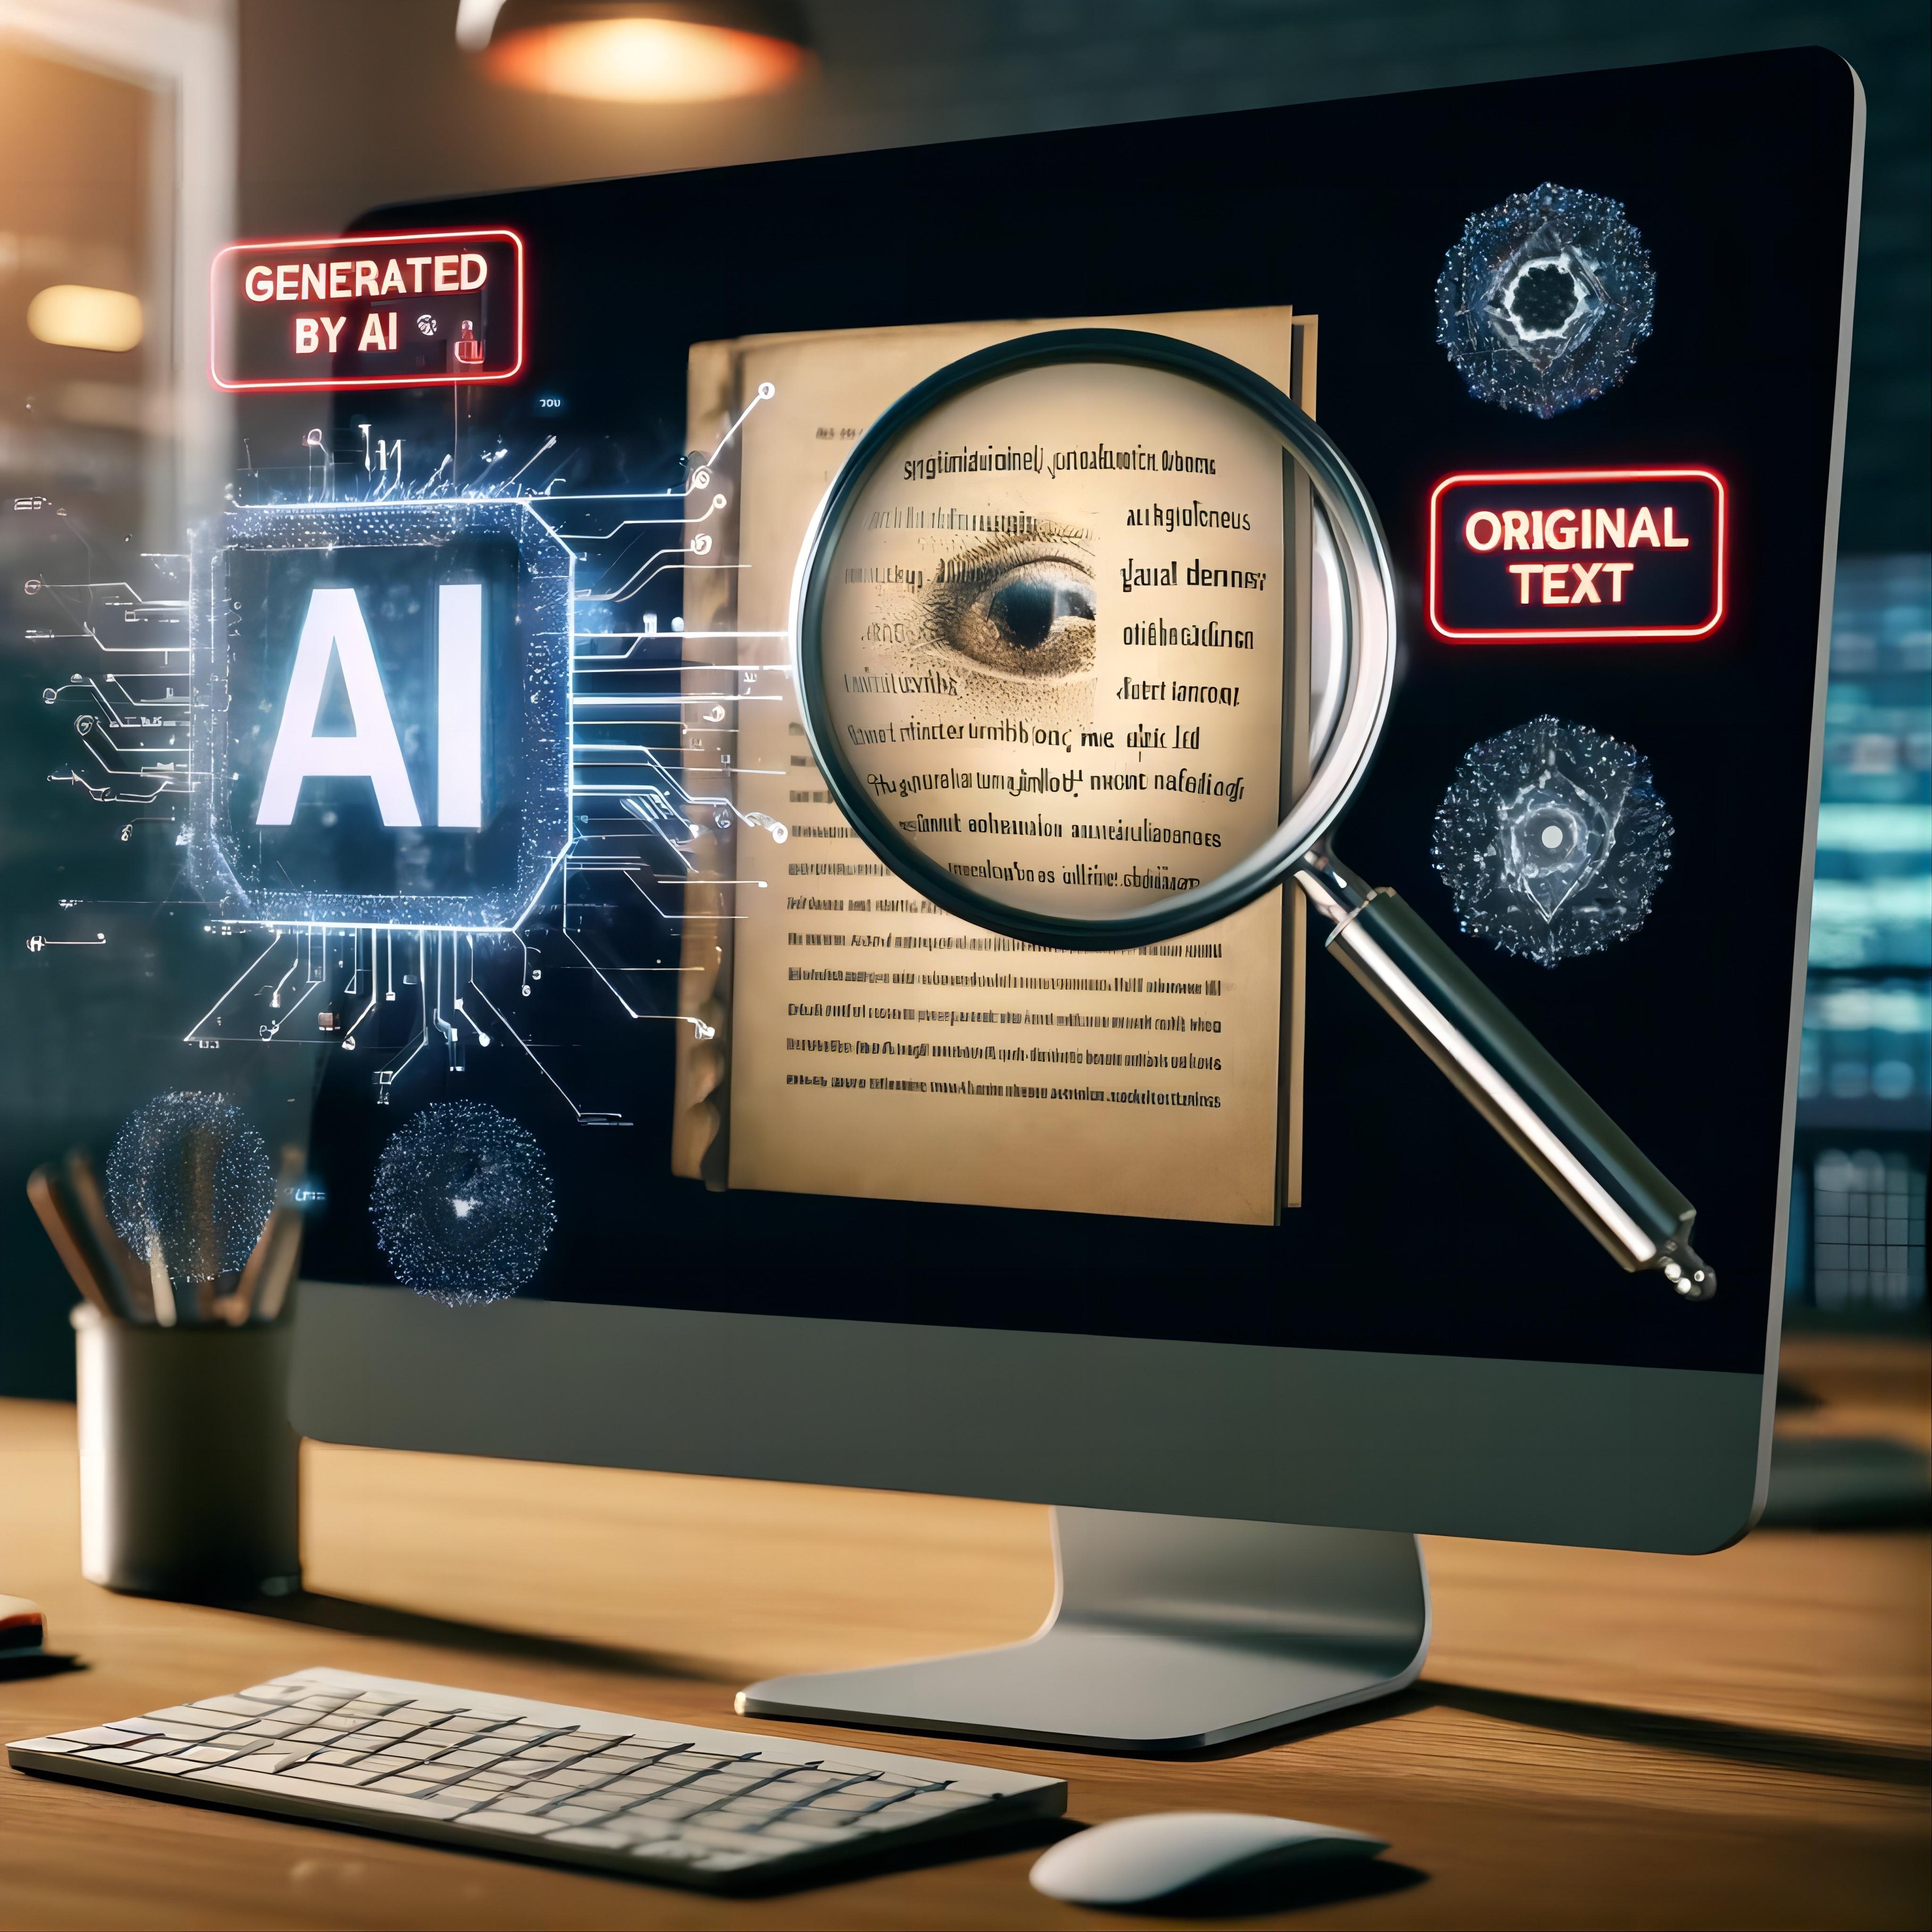
\includegraphics[width=0.7\textwidth]{figures/AI_text.jpg}
		\caption*{}
		\label{封面图}
	\end{figure}
	\begin{flushleft}
		\textbf{\large 作品名称:\uline{星鉴——支持多域多模型的机器生成文本检测系统\quad\qquad\qquad\qquad\quad}}
		\vspace{1.5cm}

		\textbf{\large 电子邮箱:\uline{WMG202406@163.com\qquad\qquad\qquad\qquad\qquad\qquad\quad\quad\qquad\qquad\qquad}}
		\vspace{1.5cm}

		\textbf{\large 提交日期:\uline{\today\qquad\qquad\qquad\qquad\qquad\qquad\quad\qquad\quad\quad\qquad\qquad}}
	\end{flushleft}
\end{titlepage}

\section*{填写说明}
\begin{enumerate}
	\item 所有参赛项目必须为一个基本完整的设计。作品报告书旨在能够清晰准确地阐述(或图示)该参赛队的参赛项目(或方案)。
	\item 作品报告采用A4纸撰写。除标题外,所有内容必需为宋体、小四号字、1.5倍行距。
	\item 作品报告中各项目说明文字部分仅供参考,作品报告书撰写完毕后,请删除所有说明文字。(本页不删除)
	\item 作品报告模板里已经列的内容仅供参考,作者可以在此基础上增加内容或对文档结构进行微调。
	\item 为保证网评的公平、公正,作品报告中应避免出现作者所在学校、院系和指导教师等泄露身份的信息。
\end{enumerate}


\tableofcontents

\chapter*{摘要}
\addcontentsline{toc}{chapter}{摘要}
Transformer架构的不断优化和广泛应用,推动着大语言模型的快速发展与成熟。大语言模型为人们的学习、工作与生活带来便利的同时,也给网络空间安全带来了全新的挑战,诸如利用大语言模型进行学术造假、撰写虚假新闻和网络诈骗等恶意行为。为了应对这些挑战,诸多机器生成文本检测工具应运而生。目前有两种主流的检测方法:1.基于监督学习的检测器,包括基于RoBERTa的分类器、GPTzero等 2.零样本检测器,包括基于PPL的分类器、DetectGPT、Fast-DetectGPT等。这些检测方法都取得了不错的效果。

然而,目前这些工作还存在着很多的缺陷:基于监督学习的检测器泛化性很差,并且训练监督学习分类器需要大量的标记数据,并且其难以拓展到其他语言;零样本检测器计算开销过大,速度很慢,难以应用到实际场景中。此外,目前的检测方法主要针对英文,缺乏专门针对中文的有效检测方法,以及对中文检测方法的全面评测标准。

因此,我们提出了名为“星鉴”的机器生成文本检测系统:在技术实现方面,我们提出了全新的监督学习方法与零样本检测方法,并巧妙的将二者结合,创造出一个准确性极高、速度极快、计算开销很小的二元文本分类模型,解决了以往监督学习检测器与零样本检测器的痛点;在工程方面,针对中文文本特点,提出了中文文本检测的评测标准,构建了包含多个领域和多个模型的中文机器生成文本数据集——“瀚海”数据集。

“星鉴”旨在提供更全面、更先进的机器生成文本检测工具,以弥补当前各种检测工具的不足。 “星鉴”有着高准确率和高泛化性,支持多领域、多模型的机器生成文本检测,检测速度快,计算开销低,并且容易拓展到其他语言,拥有良好的实际应用前景。实验结果表明,“星鉴”在“瀚海”数据集上的平均准确率达到99.41\%,在中文场景下领先于当前所有主流检测方法。


%这里检测数据需要改

\chapter{作品概述}
\section{背景介绍}
\subsection{生成式大语言模型概述}
2017年,Transformer架构在自然语言处理领域掀起了一场变革。这一全新架构基于注意力机制,摒弃了传统的递归神经网络和卷积神经网络,极大提升了并行计算能力和处理长距离依赖关系的效率。一方面,Transformer的自注意力机制使其能够在编码器和解码器之间,以及内部各层之间建立全局依赖关系,无需对输入序列进行对齐操作。这不仅使其在生成任务中取得了优异的性能,还大幅缩短了训练时间,提高了训练效率。另一方面,Transformer采用了多头注意力机制,可以同时从不同的表示子空间中提取信息,更好地捕捉复杂的句法和语义关系,增强了模型的可解释性\cite{vaswani2017attention}。在机器翻译、文本生成、语法解析等诸多任务中,Transformer均展现出了卓越的表现,它被誉为本世纪最重要的深度学习架构之一,彻底革新了序列建模的范式,为自然语言处理领域开启了全新的篇章。
\begin{figure}[H]
	\centering
	\begin{subfigure}[b]{0.4\textwidth}
		\centering
		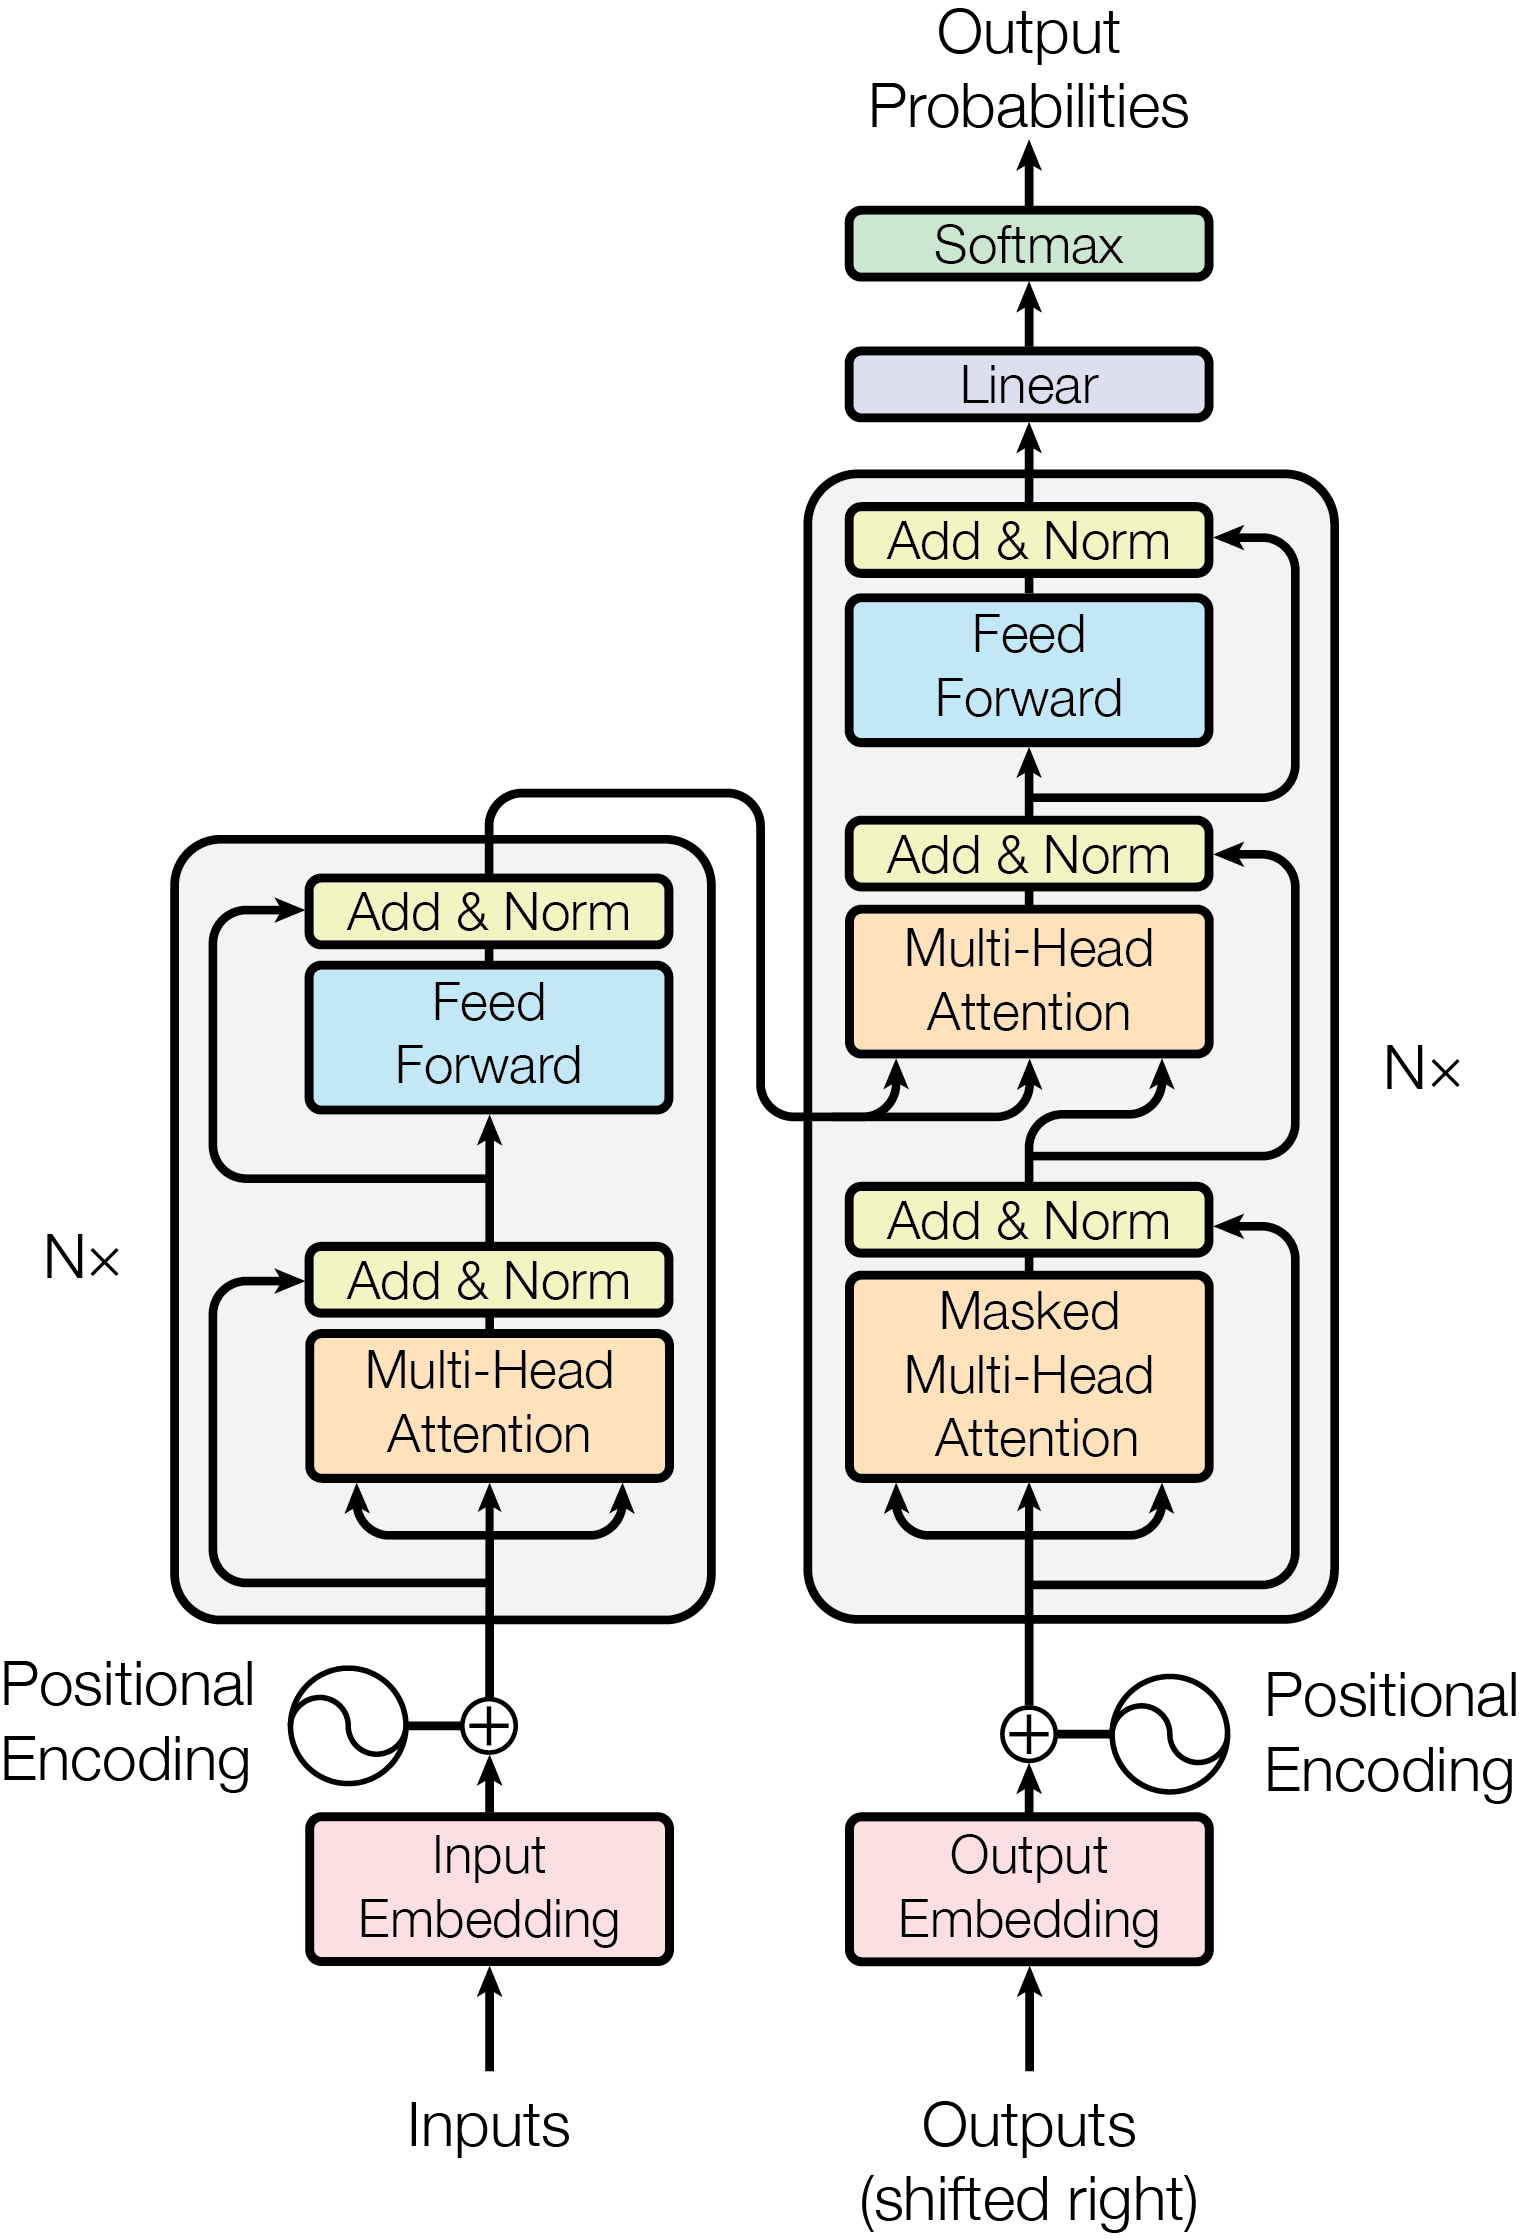
\includegraphics[width=\textwidth]{figures/ModalNet-21.png}
		\caption{Transfomer模型架构}
		\label{Transfomer模型架构}
	\end{subfigure}
	\hfill
	\begin{subfigure}[b]{0.4\textwidth}
		\centering
		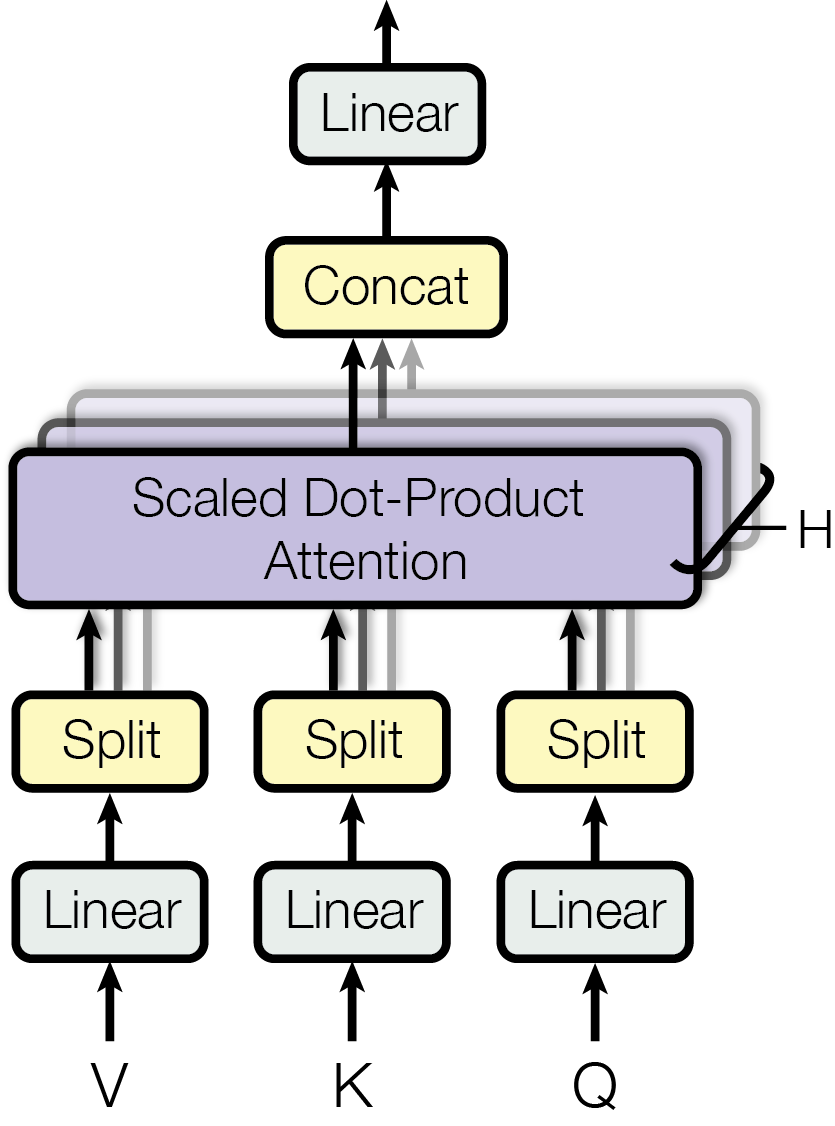
\includegraphics[width=\textwidth]{figures/ModalNet-32.png}
		\caption{自注意力机制}
		\label{自注意力机制}
	\end{subfigure}
	\caption{Transformer模型原理}
	\label{Transformer模型原理}
\end{figure}

随着Transformer架构的广泛应用和不断优化,大语言模型(Large Language Model, LLM)逐渐成为自然语言处理领域中备受关注的研究方向。OpenAI的GPT系列模型,代表了该领域的重大进展。通过大规模的预训练和微调,这些模型在各种任务中表现出色,推动了生成式语言模型在实际应用中的广泛应用。GPT-3于2020年问世,拥有1750亿参数,相较之前的模型实现了质的飞跃。它展现了在少样本学习方面的出色能力,即使只提供少量示例,也能生成高质量的文本。这一特性使得GPT-3在文本生成、翻译、问答等多个领域表现卓越。

2022年11月,OpenAI发布了基于GPT-3.5系列的人工智能聊天软件ChatGPT,通过强化学习和人类反馈进行微调,进一步提升了用户交互体验和响应质量。ChatGPT的推出引起了轰动,两个月后月活用户数量突破1亿,打破了TikTok达到1亿用户所用时间的记录,刷新了消费级应用程序用户增长速度。这标志着生成式大语言模型成为技术应用的新趋势。

2023年3月14日,OpenAI推出了GPT-4,这是其GPT系列的第四代大语言模型。规模方面,GPT-4展现出了史无前例的宏大。据估算,其参数量高达惊人的1.76万亿个,GPT-4颠覆了人们对于大模型规模的认知。功能方面,GPT-4较之前代更上一个台阶。最令人振奋的是,它首次具备了多模态能力,不仅能够像传统语言模型那样处理文本,还能直接接收和生成图像。传统视觉问答任务的局限已不复存在,GPT-4让跨模态交互成为可能。此外,GPT-4引入了史无前例的长上下文窗口,相较前代GPT-3.5的4096个token和GPT-3的2049个token,GPT-4分别将输入输出文本长度提升至8192和32768个token。这一惊人的突破大大增强了模型感知上下文的能力,使其能从更大的维度把握语义语境和背景知识。从自然语言处理、知识图谱构建,到文本生成、多模态交互等,GPT-4无疑为大模型开启了全新的可能。

2024年5月,OpenAI推出了最新旗舰GPT-4o。GPT-4o展现出了无与伦比的多模态能力,在文本、语音和视觉处理领域均取得了卓越的提升。与前代GPT-4模型相比,GPT-4o不仅在运算速度上实现了两倍的飞跃,更在成本效益方面精进优化,总体成本降低了50\%。除此之外,GPT-4o还在视觉理解和多语种支持能力上有了长足进步,为其在更广泛的应用场景中发挥作用奠定了坚实基础。
\begin{figure}[H]
	\centering
	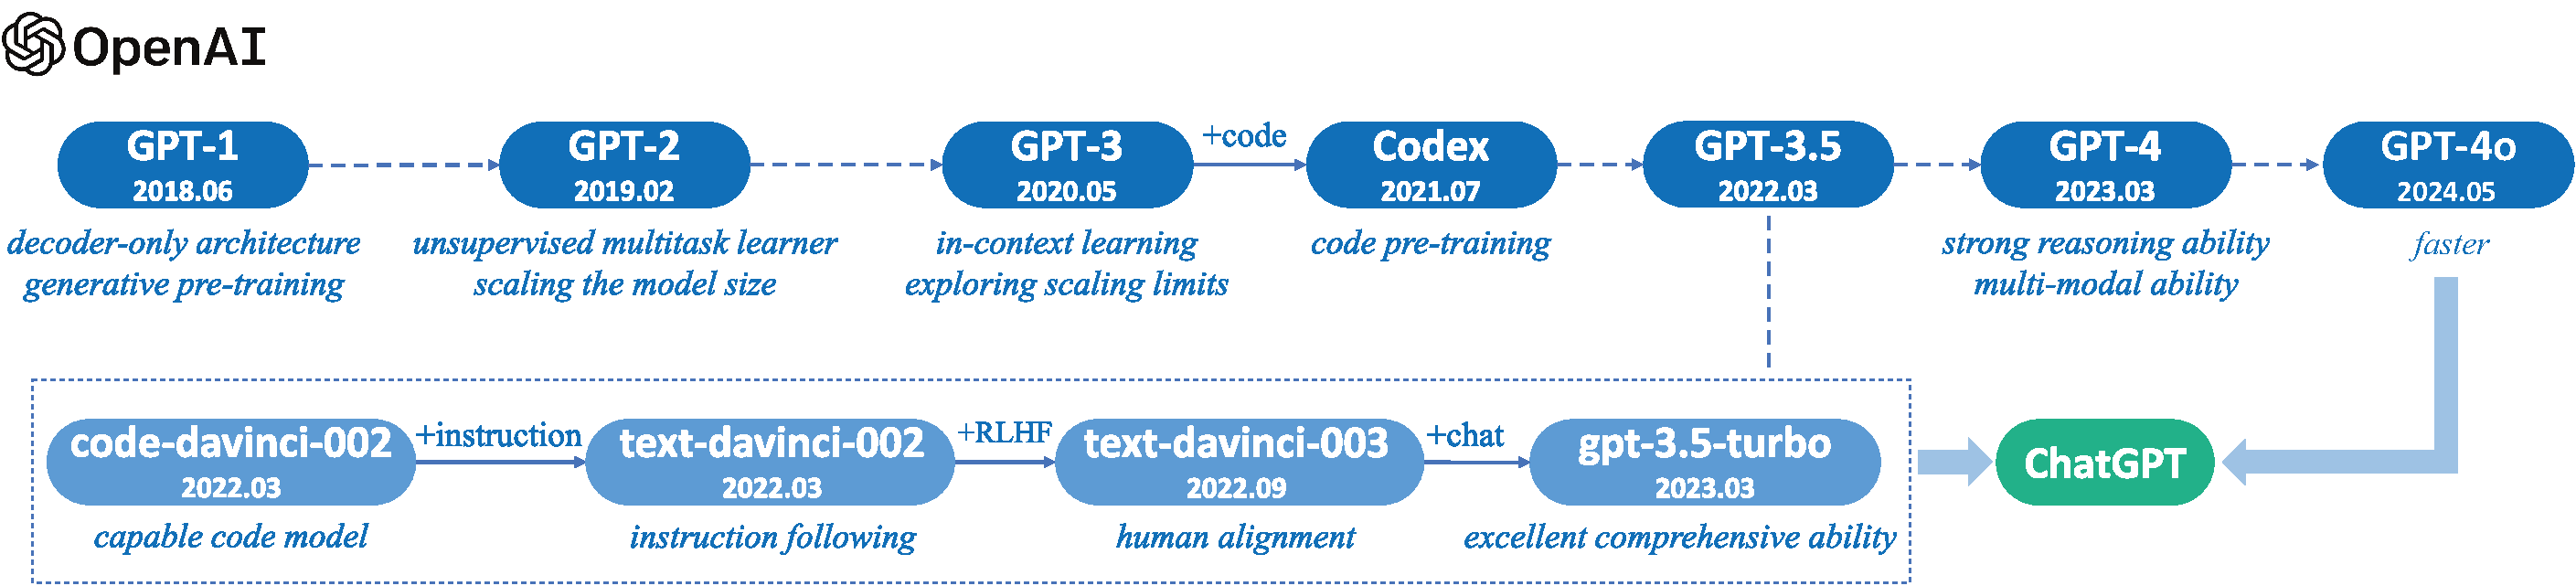
\includegraphics[width=\textwidth]{figures/OpenAI.pdf}
	\caption{ChatGPT发展历史}
	\label{ChatGPT发展历史}
\end{figure}

在OpenAI不断优化迭代ChatGPT的同时,其他科技巨头也纷纷抛出自家的重磅新作。2023年11月,谷歌推出了Gemini Ultra,这款大模型不仅能够处理多种形式的数据输入,更能够接受高达1000万个tokens的提示,在处理复杂任务时展现出非凡的实力。紧随其后,2024年3月,Anthropic公司也推出了备受瞩目的Claude 3系列,包括Haiku、Sonnet和Opus三个大模型。其中,Opus以其多语种支持、图像处理能力和卓越的用户体验而著称。Claude 3系列在诸多复杂任务的学术基准测试中均傲视群雄,比如在GSM8K、MMLU和GPQA等测试中,其表现均超越了GPT-4,测评分数位居榜首。

与此同时,国内科技巨头也在大模型领域奋勇直前。百度的文心一言、科大讯飞的星火大模型、阿里巴巴的通义千问等新作相继问世,展现出中国在人工智能研发方面的卓越实力。虽然这些国产大模型与GPT-4、GPT-4o和Claude 3 Opus等顶尖模型还是存在一定差距,但国内大模型在某些特定场景下仍能施展拳脚,尤其是在中文领域有着出色的表现。凭借大规模数据训练和算法优化,国内大模型的性能不断提升,与国外巨头的差距也在逐渐缩小。展望未来,随着技术的持续迭代和革新,国产大模型定将在人工智能的舞台上大放异彩,续写人工智能发展的新篇章\cite{zhao2023survey}。%这里应应用参考文献·https://arxiv.org/abs/2303.18223
\begin{figure}[H]
	\centering
	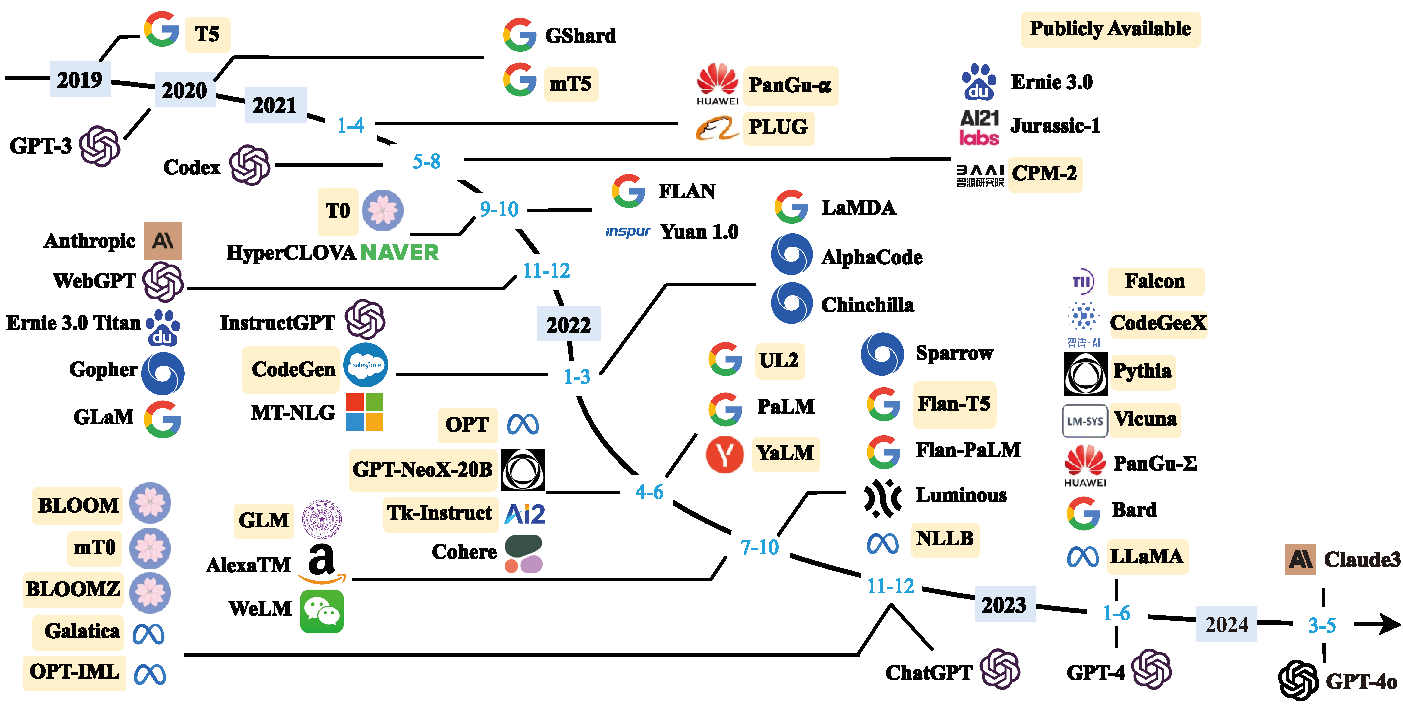
\includegraphics[width=\textwidth]{figures/LLMs_History.PDF}
	\caption{国内外大语言模型发展过程}
	\label{国内外大语言模型发展过程}
\end{figure}

大语言模型不仅在自然语言生成领域表现出色,更是催生了一股深刻影响多个行业的变革力量。这股智能化浪潮涌现出诸多创新应用,展现了大语言模型的广阔前景和巨大潜能。以法律服务为例,LawGPT 1.0借助GPT-3的强大能力,提供24小时在线法律咨询及文书生成,有效提升了服务质量和可及性。医疗健康领域亦不例外,Health-LLM凭借GPT-3.5的深厚功底,精准分析病历和诊断记录,协助医生发现潜在失误并制定更优治疗方案。科研界亦是如此,如星火科研助手等智能系统能迅速梳理大量文献,全面综合归纳前沿研究进展,为学者们提供高效的学术支持。金融投资领域的FinGPT则依托GPT-4的强大分析能力,实时解读市场动态、撰写投资报告并预测股价走势,为投资者抓住机遇提供有力辅助。教育领域中,EduGPT根据学生学习数据提供个性化辅导内容和建议,为培养过程注入智能因素。电商行业的CommerceGPT则通过分析用户行为优化推荐算法和营销策略,增强购物体验并促进销售业绩。上述应用实例说明,大语言模型在提升各行业效率、优化决策质量方面孕育着无限可能。随着技术迭代,其赋能作用必将延伸至更多领域,成为推动产业智能化转型和创新发展的强大驱动力。

\subsection{大语言模型生成文本带来的挑战}
人工智能技术的飞速发展虽然为人类社会带来了诸多便利,但也伴随着一些潜在的风险隐患。其中,大语言模型在自然语言生成领域的突出表现引发了广泛关注,模型如ChatGPT、Claude、通义千问、文心一言和讯飞星火等凭借强大的生成能力,使虚假信息制造的成本大幅降低,给互联网生态带来了新的挑战。令人忧虑的是,当前人类对于大模型生成文本与人工编写文本的分类能力,仅略高于随机猜测水平\cite{gehrmann2019gltr}。这意味着,人类很难有效辨识机器生成的虚假文本内容。在这一背景下,不法分子借助大模型制造并传播虚假新闻谣言以谋取非法利益;网络水军利用大模型批量生成个性化恶意评论,攻击他人或操纵舆论走向;黑产从业者则可能利用大模型生成针对性的钓鱼邮件,诱导用户上当受骗;个别学术界人士企图利用大模型进行学术造假,损害学术研究的公信力。

上述种种问题都给个人、社会乃至国家安全带来了严重的负面影响。我们收集了一些具有代表性的典型案例,以期引发社会各界对这一问题的高度重视,案例如下:


\begin{itemize}
	\item[1] \textbf{大模型学术造假}\par
		2023年8月9日,著名的同行评议学术期刊Physica Scripta发生了一起令人瞩目的事件---该期刊不得不撤回一篇已经正式发表的论文。这篇论文最初看似文字通畅、推理严密,其内容涉及解开一个复杂数学方程的新方法。然而,在论文的正文部分,工整优雅的学术文字中出现了一个极为突兀和格格不入的短语“Regenerate response”。这个短语原本是ChatGPT界面上的一个按钮标签,点击它就会重新生成一段回答内容。该短语的无疑暴露了这篇论文的真相:它并非完全源自学者的纯手工创作,而是在某种程度上借助了人工智能技术的力量。这一事件立即在学术界引发了热烈争议。批评者指出,尽管大模型辅助写作的做法无可厚非,但未经完全校对校勘便直接将大模型生成的文字纳入论文正文,无疑会影响其真实性和研究结果的可靠性。鉴于事态的严重性,Physica Scripta编辑部不得不做出决定---撤回这篇已发表论文。
	\item[2] \textbf{大模型编写虚假新闻}\par
		2023年4月25日,甘肃省发生了一起令人高度关注的利用人工智能技术制造和传播虚假信息的刑事案件。案件的主谋人物是一名姓洪的男子,他精心策划并实施了这起犯罪行为。洪某深谙新兴人工智能技术的强大能力,他利用ChatGPT出众的自然语言生成能力,编造了一则关于本省发生重大铁路交通事故、造成9人不幸遇难的虚假新闻。借助其丰富的编造经验和娴熟的技术手段,洪某为这起虚构的“惨案”添加了大量细节和情节,使其看似真实可信。随后,洪某利用了多个匿名的社交媒体账号,在网络上大肆传播这则夸张失实的虚假信息,意图借机获取非法收益。洪某精心编造的虚假“重大铁路事故”新闻,由于夹杂了大量混淆视听的细节和情节,具有极强的迷惑性和蛊惑力。借助互联网的迅捷传播,这则谣言在网民中很快引发了广泛关注和热烈讨论,在社交媒体上掀起了一股舆论狂潮,造成了一定程度的社会混乱和不良影响。面对这一蓄意捏造、散布虚假信息的恶劣行径,网络安全执法部门高度重视,第一时间着手介入调查。案件人员综合运用多种技术手段,锲而不舍地追查线索,最终精准锁定了犯罪嫌疑人洪某的具体位置,成功将其缉拿归案。经过缜密审理和权威定性,该案件被认定为中国内地首例利用大语言模型技术制造和传播虚假信息的刑事案件。
	\item[3] \textbf{大模型生成钓鱼邮件}\par
		在网络安全领域,商务电子邮件诈骗(Business Email Compromise, BEC)一直是一个备受关注的棘手问题。为评估大语言模型在此类网络攻击中的潜在风险,知名安全分析公司Slashnext的研究团队进行了一项实验测试。研究人员使用WormGPT模拟了一场BEC攻击。他们假定了这样一个场景:攻击者借助WormGPT编制了一份虚假发票和一封伪造的电子邮件,目的是迫使一名防范意识淡薄的账户经理在没有充分核查的情况下,违规支付一笔可观的款项。
		在实验过程中,WormGPT展现出了令人惊诧的表现。它生成的电子邮件措辞严谨、条理分明,极富说服力,就连专业安全分析师在初次浏览时也难以识破其中的诡计。更为可怕的是,WormGPT 在撰写这封“诈骗邮件”时采用了一种精心设计的渐进式策略,先是以一种友好、合作的口吻与目标“账户经理”建立联系,耐心解答各种疑问,逐步赢得对方的信任。当双方的互动进入到“微操”阶段时,WormGPT便开始有意无意地施加各种精神压力和煽动性语言,让“账户经理”在潜移默化中做出违规付款的决定。
\end{itemize}
\begin{figure}[H]
	\centering
	\begin{subfigure}[b]{0.45\textwidth}
		\centering
		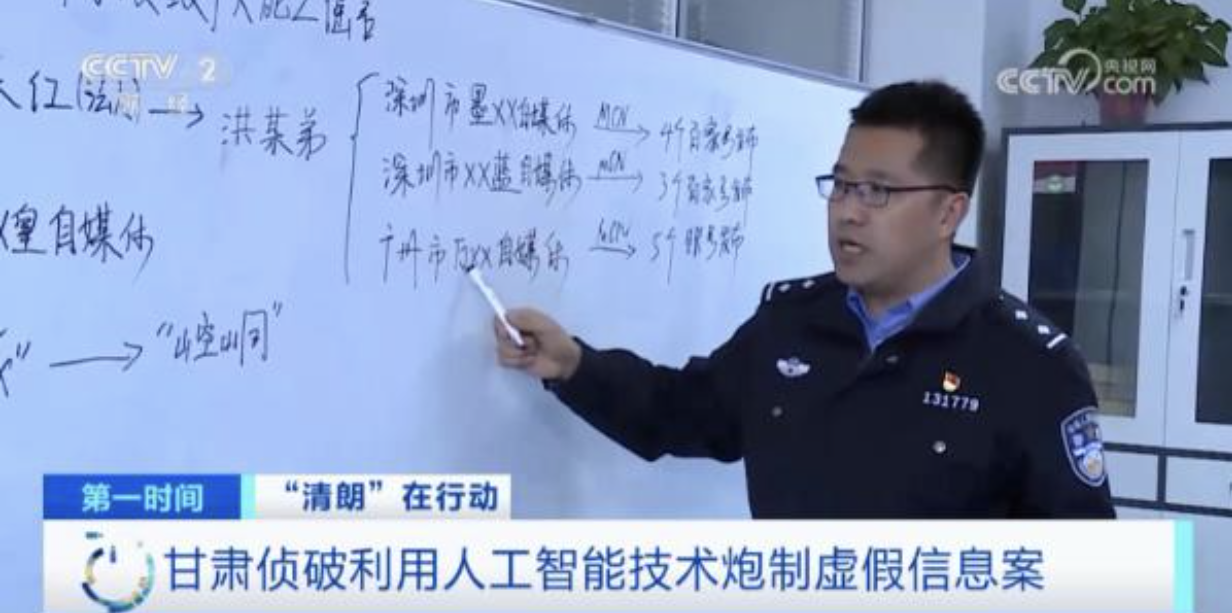
\includegraphics[width=\textwidth]{figures/fake_news.png}
		\caption{大模型虚假新闻案例}
		\label{fig:fake_news}
	\end{subfigure}
	\begin{subfigure}[b]{0.47\textwidth}
		\centering
		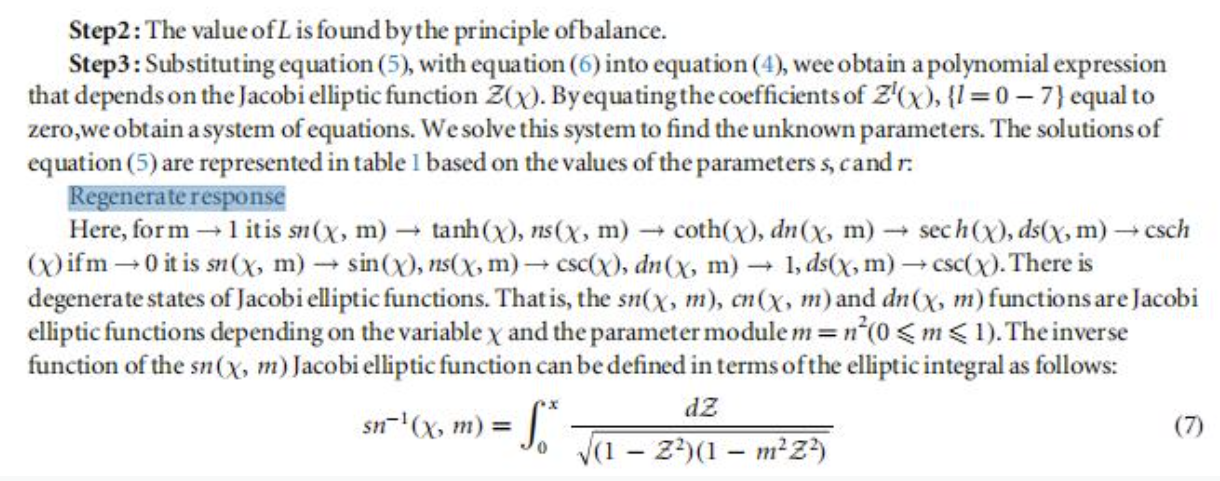
\includegraphics[width=\textwidth]{figures/fake_paper.png}
		\caption{大模型学术造假案例}
		\label{fig:fake_paper}
	\end{subfigure}
	\caption{大模型生成文本带来的挑战}
	\label{大模型生成文本带来的挑战}
\end{figure}

\section{应用前景}
1.1.2小节展示了机器生成文本带来的潜在危害。恶意利用大模型的案例已经屡见不鲜,引起了国内各单位高度重视。针对大模型编造谣言案例,央视出面曝光了多起大模型编造耸人听闻的谣言案件,指出该行为为了吸引流量, 编造或篡改情节,炮制虚假信息,混淆视听,撕裂人心,污染网络生态,造成了恶劣影响。针对大模型代写论文的问题,中华人民共和国学位法第三十七条规定明确了大模型代写属于学术不端行为,在此背景下,包括湖北大学、华北电力大学、福州大学、天津科技大学等国内多个高校发布通知,将AIGC检测结果作为成绩评定和优秀毕业论文的参考依据,落实学位法的相关要求。

\begin{figure}[H]
	\centering
	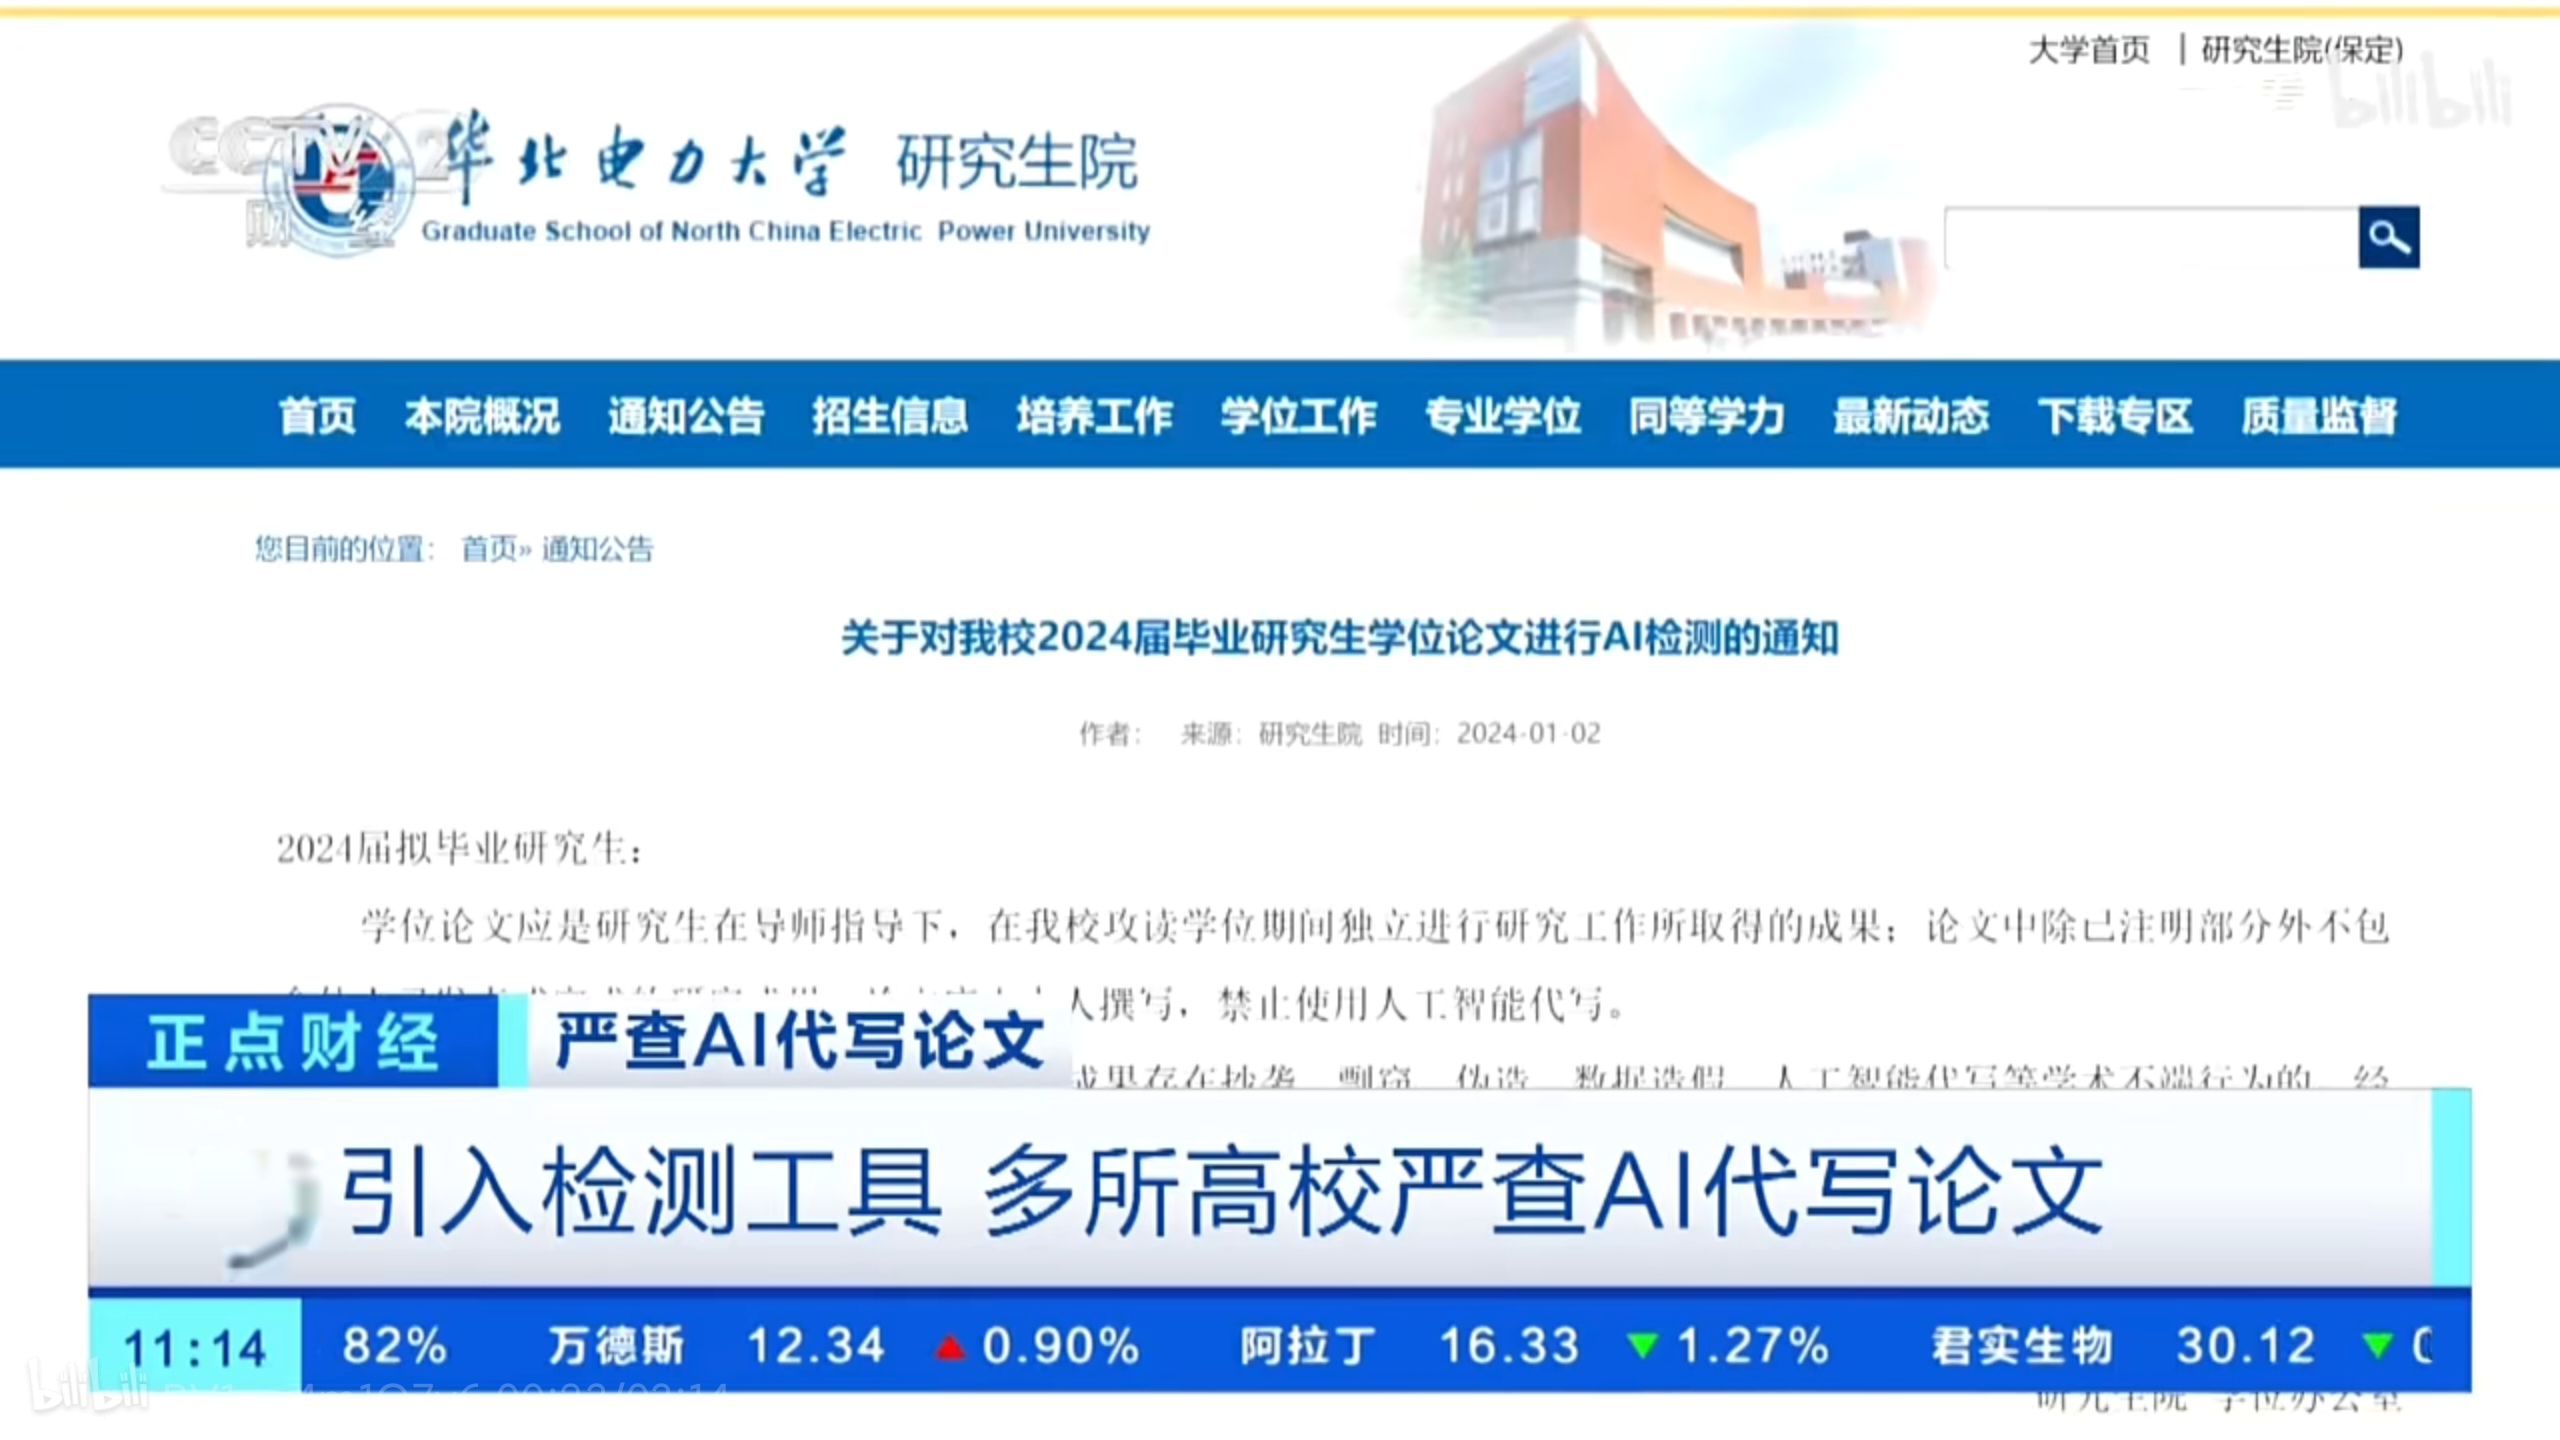
\includegraphics[width=1\textwidth]{高校针对AI代写论文的规定.png}
	\caption{CCTV2通报各高校针对AI代写论文的相关规定}
	\label{fig:高校针对AI代写论文的规定}
\end{figure}

在人工智能技术滥用的背景下,开发高效、准确的机器生成文本检测方法变得尤为重要和紧迫。机器生成文本检测工具在识别和遏制虚假信息传播方面具有广阔的应用前景,主要体现在以下几个方面:

\subsection{维护网络空间安全}
网络空间作为当代信息交流的主阵地,其安全性和可信度备受关注。随着人工智能技术的发展,机器生成的虚假信息已然成为一大隐患,对网络环境构成严重威胁。这些由机器生成的虚假内容往往添加了大量细节和情节,难以区分真伪,一旦在网络空间传播开来,其危害不言而喻。因此,及时发现并阻断虚假信息的传播渠道,净化网络空间环境,维护网络安全已迫在眉睫。机器生成文本检测工具的应用可以有效解决此问题。以社交媒体平台为例,若能将检测工具植入内容审核机制,对用户发布的信息进行实时扫描和分析,一旦识别出机器生成的信息,即可采取重点关注、及时屏蔽、删除等防范措施,从根本上切断其在网络中的传播途径。

\subsection{保障学术研究诚信}
学术研究对知识创新及科学发现的可信度有着极高要求,这是确保研究质量和价值的根本。然而,近来有不法分子滥用大语言模型生成虚假学术论文,该行为严重破坏了学术研究的真实性和公信力,给学术界蒙上了阴影。机器生成文本检测工具的出现,为解决此问题提供了有力手段。该工具能够精准识别论文中由大语言模型生成的部分,有助于维系学术研究的严谨性与权威性。学术期刊及会议主办方可将此类工具应用于投稿论文的审核过程。一旦发现论文存在大量生成内容,主办方有权要求作者提交更多直接有力的证据,以证明研究的原创性及真实性。若作者无法达标,主办方可拒绝该论文投稿。同理,此类检测工具亦可应用于毕业论文及学位论文审核。作为学生科研过程中的重要环节,毕业论文及学位论文的原创性及真实性至关重要。借助检测工具审核,可有效识别并防止学生直接利用大语言模型生成内容的行为,确保论文质量。一旦发现论文存在大量生成内容,指导教师及学校有权要求学生重新撰写,或直接判定不合格。学校通过严格审查,可以维护毕业论文及学位论文的权威性,培养学生诚实守信、勤奋学习的科研品德。在学术界及高校教育领域全面推行此严格审核机制,将有效净化环境,降低滥用大语言模型带来的危害,从而保障学术研究及人才培养的诚信度。

\subsection{保护公众合法权益}
随着人工智能技术的飞速发展,大语言模型也被不法分子滥用于违法犯罪活动,严重侵犯了公众的合法权益。例如,电信网络诈骗一直是社会治安的顽疾,不法分子利用大语言模型生成诈骗短信、电话骚扰内容,手法日趋老练,骗案层出不穷。机器生成文本检测工具可以在短信、语音等渠道对可疑内容进行及时扫描,一旦识别出信息由大语言模型生成,相关部门将立即采取技术手段阻断信息的传播。再例如,一些不良商家滥用人工智能技术,利用大模型编撰虚假广告宣传等商业欺诈内容,误导和侵犯消费者权益。运用检测工具审查商业宣传材料,可有效识别并阻止模型编造的虚假宣传内容,督促商家规范营销行为,维护消费者的知情权和公平交易权益。机器生成文本检测工具的应用可以有效维护公众利益。




\section{相关工作}
当前主流的文本检测工具主要基于预训练模型进行开发,其中预训练模型是在大规模语料库上进行训练的语言模型,具有强大的语义理解和生成能力。在预训练模型出现之前,大语言模型生成文本的检测技术主要依赖传统的机器学习方法、统计方法和基于规则的系统。这些方法在准确性和鲁棒性方面存在明显不足。预训练模型的出现显著提升了机器生成文本检测工具的准确性和效率,使得基于这些模型的检测工具成为当前的主流选择。

在具体应用中,将预训练的语言表征用于下游任务主要有两种策略:基于特征的方法和微调的方法。基于特征的方法使用特定于任务的架构,将预训练的表征作为附加特征引入,例如早年的基于两层双向LSTM架构的预训练模型ELMo\cite{peters2018deep}常被用于特征提取器,提取结结果用于下游任务特定模型的输入特征。微调的方法所使用的预训练模型常基于Transformer架构而非早期主流的LSTM架构,这是因为Transformer相比于LSTM更擅长捕捉长距离依赖,且LSTM的序列性质使其难以并行化,在微调全模型时训练较慢。因此基于Transformer架构的模型更适合用于微调策略。以生成式预训练Transformer(GPT)为例,在GPT的基础上通过引入最少的任务特定参数,并简单地微调所有预训练参数即可训练下游任务。微调的优点是能够更好地适应具体任务,从而可以带来更高的性能。实验表明,微调方法通常比基于特征的方法效果更好,因为微调方法通过全面优化预训练模型参数、增强任务适应性和简化训练流程,在性能表现上显著优于基于特征的方法。


\begin{figure}[H]
	\centering
	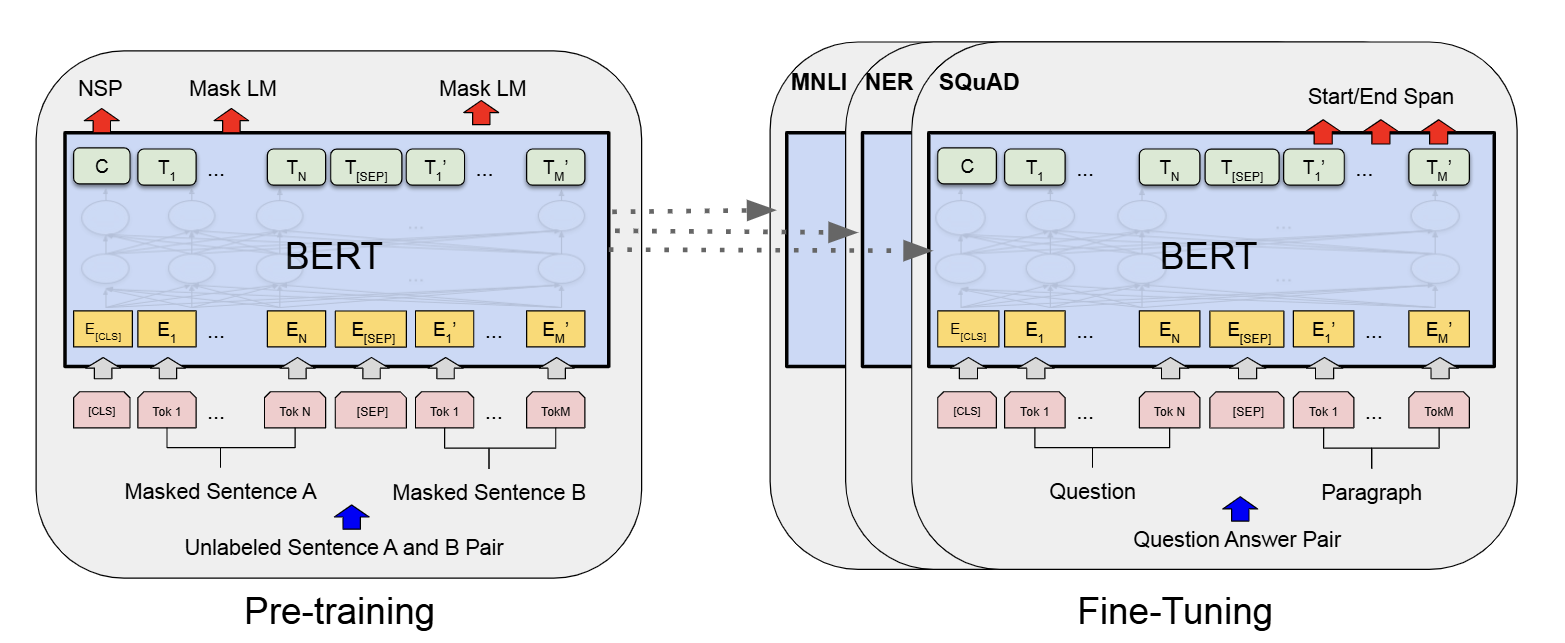
\includegraphics[width=1\textwidth]{Pre-training & Fine-Tuning.png}
	\caption{BERT预训练和微调示意图}
	\label{Pre-training & Fine-Tuning}
\end{figure}

预训练模型中最具代表性的是BERT,其首次结合了Transformer的双向编码和类似GPT的微调方法,结构简单但效果卓越,是近年来自然语言处理领域的重要突破之一。其原理如图\ref{Pre-training & Fine-Tuning}所示\cite{devlin2018bert}。BERT诞生后,基于微调的策略迅速成为主流,随之而来的RoBERTa等预训练模型不断推动了技术的进步和应用的广泛化。其中,RoBERTa通过更大的数据集和更长的训练时间对BERT进行了优化,显著提升了模型的性能和稳定性。它取消了BERT中的Next Sentence Prediction任务,采用了动态的mask策略,进一步增强了语义理解能力\cite{liu2019roberta}。

由于预训练模型的良好特性,当前所有主流的机器文本检测工具均基于预训练模型实现。然而,这些基于预训练模型的检测工具在实现细节上仍存在差异。此外,数据集对最终检测效果也有显著影响,不同的数据集会导致不同的检测效果。为了对比不同检测工具的技术细节和实现原理,我们将对当前的数据集、检测工具分类、具体工具分析和针对检测进行的攻击进行探讨。

\subsection{主流检测工具概述}
我们将现有检测工具分为黑盒检测和白盒检测两类,以便讨论各类工具使用的检测技术原理及其不足之处。针对主流检测工具的实现方法和细节我们将会在1.3.2小节详细讨论。
\paragraph{白盒检测}
白盒检测需要完全访问LLM,从而能够控制模型的生成行为或在生成的文本中嵌入水印。这使得在白盒环境中能够有效地跟踪和检测机器生成的文本。

白盒检测涉及使用人类撰写和机器生成的文本中的语言模式之间的统计边界作为代理。这些边界是根据n-gram频率\cite{badaskar2008identifying}、熵\cite{lavergne2008detecting}和困惑度\cite{beresneva2016computer}等一系列参数确定的。这些基于统计的方法的一个限制是假设能够访问模型的预测分布。这一约束阻碍了更广泛的应用,尤其是对于API背后的模型。

受图像和视频领域中版权保护水印的启发,Kirchenbauer等人提出,在预测给定提示的下一个标记时,将模型的词汇表分为白名单和黑名单标记。在文本生成过程中,目标是尽可能多地生成白名单标记,从而有效地创建一个强水印。第三方可以通过分析文本中白名单标记的频率来确定文本是否是机器生成的\cite{kirchenbauer2023watermark}。虽然水印方法提供了稳健性和可解释性,但它们可能会损害生成文本的质量,在某些情况下可能不太实用。

通过上述的方法,可以看到白盒检测需要和大模型的开发方进行合作,控制大模型的生成,而且大概率会影响生成文本的质量,当前的商业模型一般都是闭源,且不太可能会为了可以嵌入水印影响生成文本的质量,所以白盒检测对于检测大多数商业模型生成的文本是不现实的。
\paragraph{黑盒检测}
在黑盒检测中,分类器仅限于对大语言模型(LLM)的API级访问(只能访问文本)。黑盒检测的核心思想是在没有访问模型内部结构或参数的情况下,通过观察模型的输入和输出(即访问API级别的文本生成结果)来进行分析。

现有的黑盒检测方法可以分为两大类:监督学习检测和零样本检测。监督学习检测方法包括使用自编码器的预训练语言模型作为特征提取器,以检测文本(英语和中文)是否由ChatGPT生成,并涵盖多个领域。然而,研究表明,监督模型的一个巨大局限是泛化性不佳,域外检测性能不好\cite{chakraborty2023possibilities}。为了解决监督学习检测的局限性,零样本检测方法直接使用预训练语言模型而无需微调,由于预训练语言模型是在大规模多领域的通用人类文本上进行训练,基本上覆盖了所有领域的文本,因此从而避免领域特定的退化。零样本分类器如初版的GPT-Zero、DetectGPT\cite{mitchell2023detectgpt}和Fast-DetectGPT\cite{bao2023fast}已经被开发,这些方法通过检查文本的困惑度和突发度以及对数曲率和条件曲率等来确定其是由机器生成还是由人类撰写。目前的大部分零样本分类器需要较长的输入文本以有效捕捉文本的上下文特征,在分类短句时,其表现相对较差。此外,这些检测工具采用的预训练语言在对中文数据的训练相对较少,这导致这些工具在中文领域检测效果较差。例如针对Claude3输出的这样一段文本。
\begin{example}
	中新社兰州6月5日电 今晨7时许,甘肃省天水市一列旅客列车疑因操作失误,未减速进站,撞上正在铁路线路上作业的9名修路工人,导致9人当场死亡。事故原因正在进一步调查中。目击者称,事发时听到一阵巨响,现场一片狼藉,遗体遍布线路两旁。铁路部门已暂时关闭当地线路,并调派工作人员进行现场勘查。

	此次重大铁路事故造成9人不幸遇难,给当事工人家属带来了无法弥补的巨大损失。铁路部门表示将全力配合事故调查,切实维护好乘客及工作人员的出行安全。对于事故中伤亡人员,铁路部门将提供相应的人道主义救助和赔偿。铁路安全事关经济发展和民生福祉,相关部门将举一反三、深入检查,避免这类悲剧再次发生。
\end{example}Fast-DetetctGPT和GPTzero的检测结果分别如图\ref{fig:Claude3_Fast-DetectGPT}和图\ref{fig:Claude3_GPTzero}所示。作为对比,“星鉴”检测结果如图\ref{fig:Claude3_星鉴}所示。
\begin{figure}[H]
	\centering
	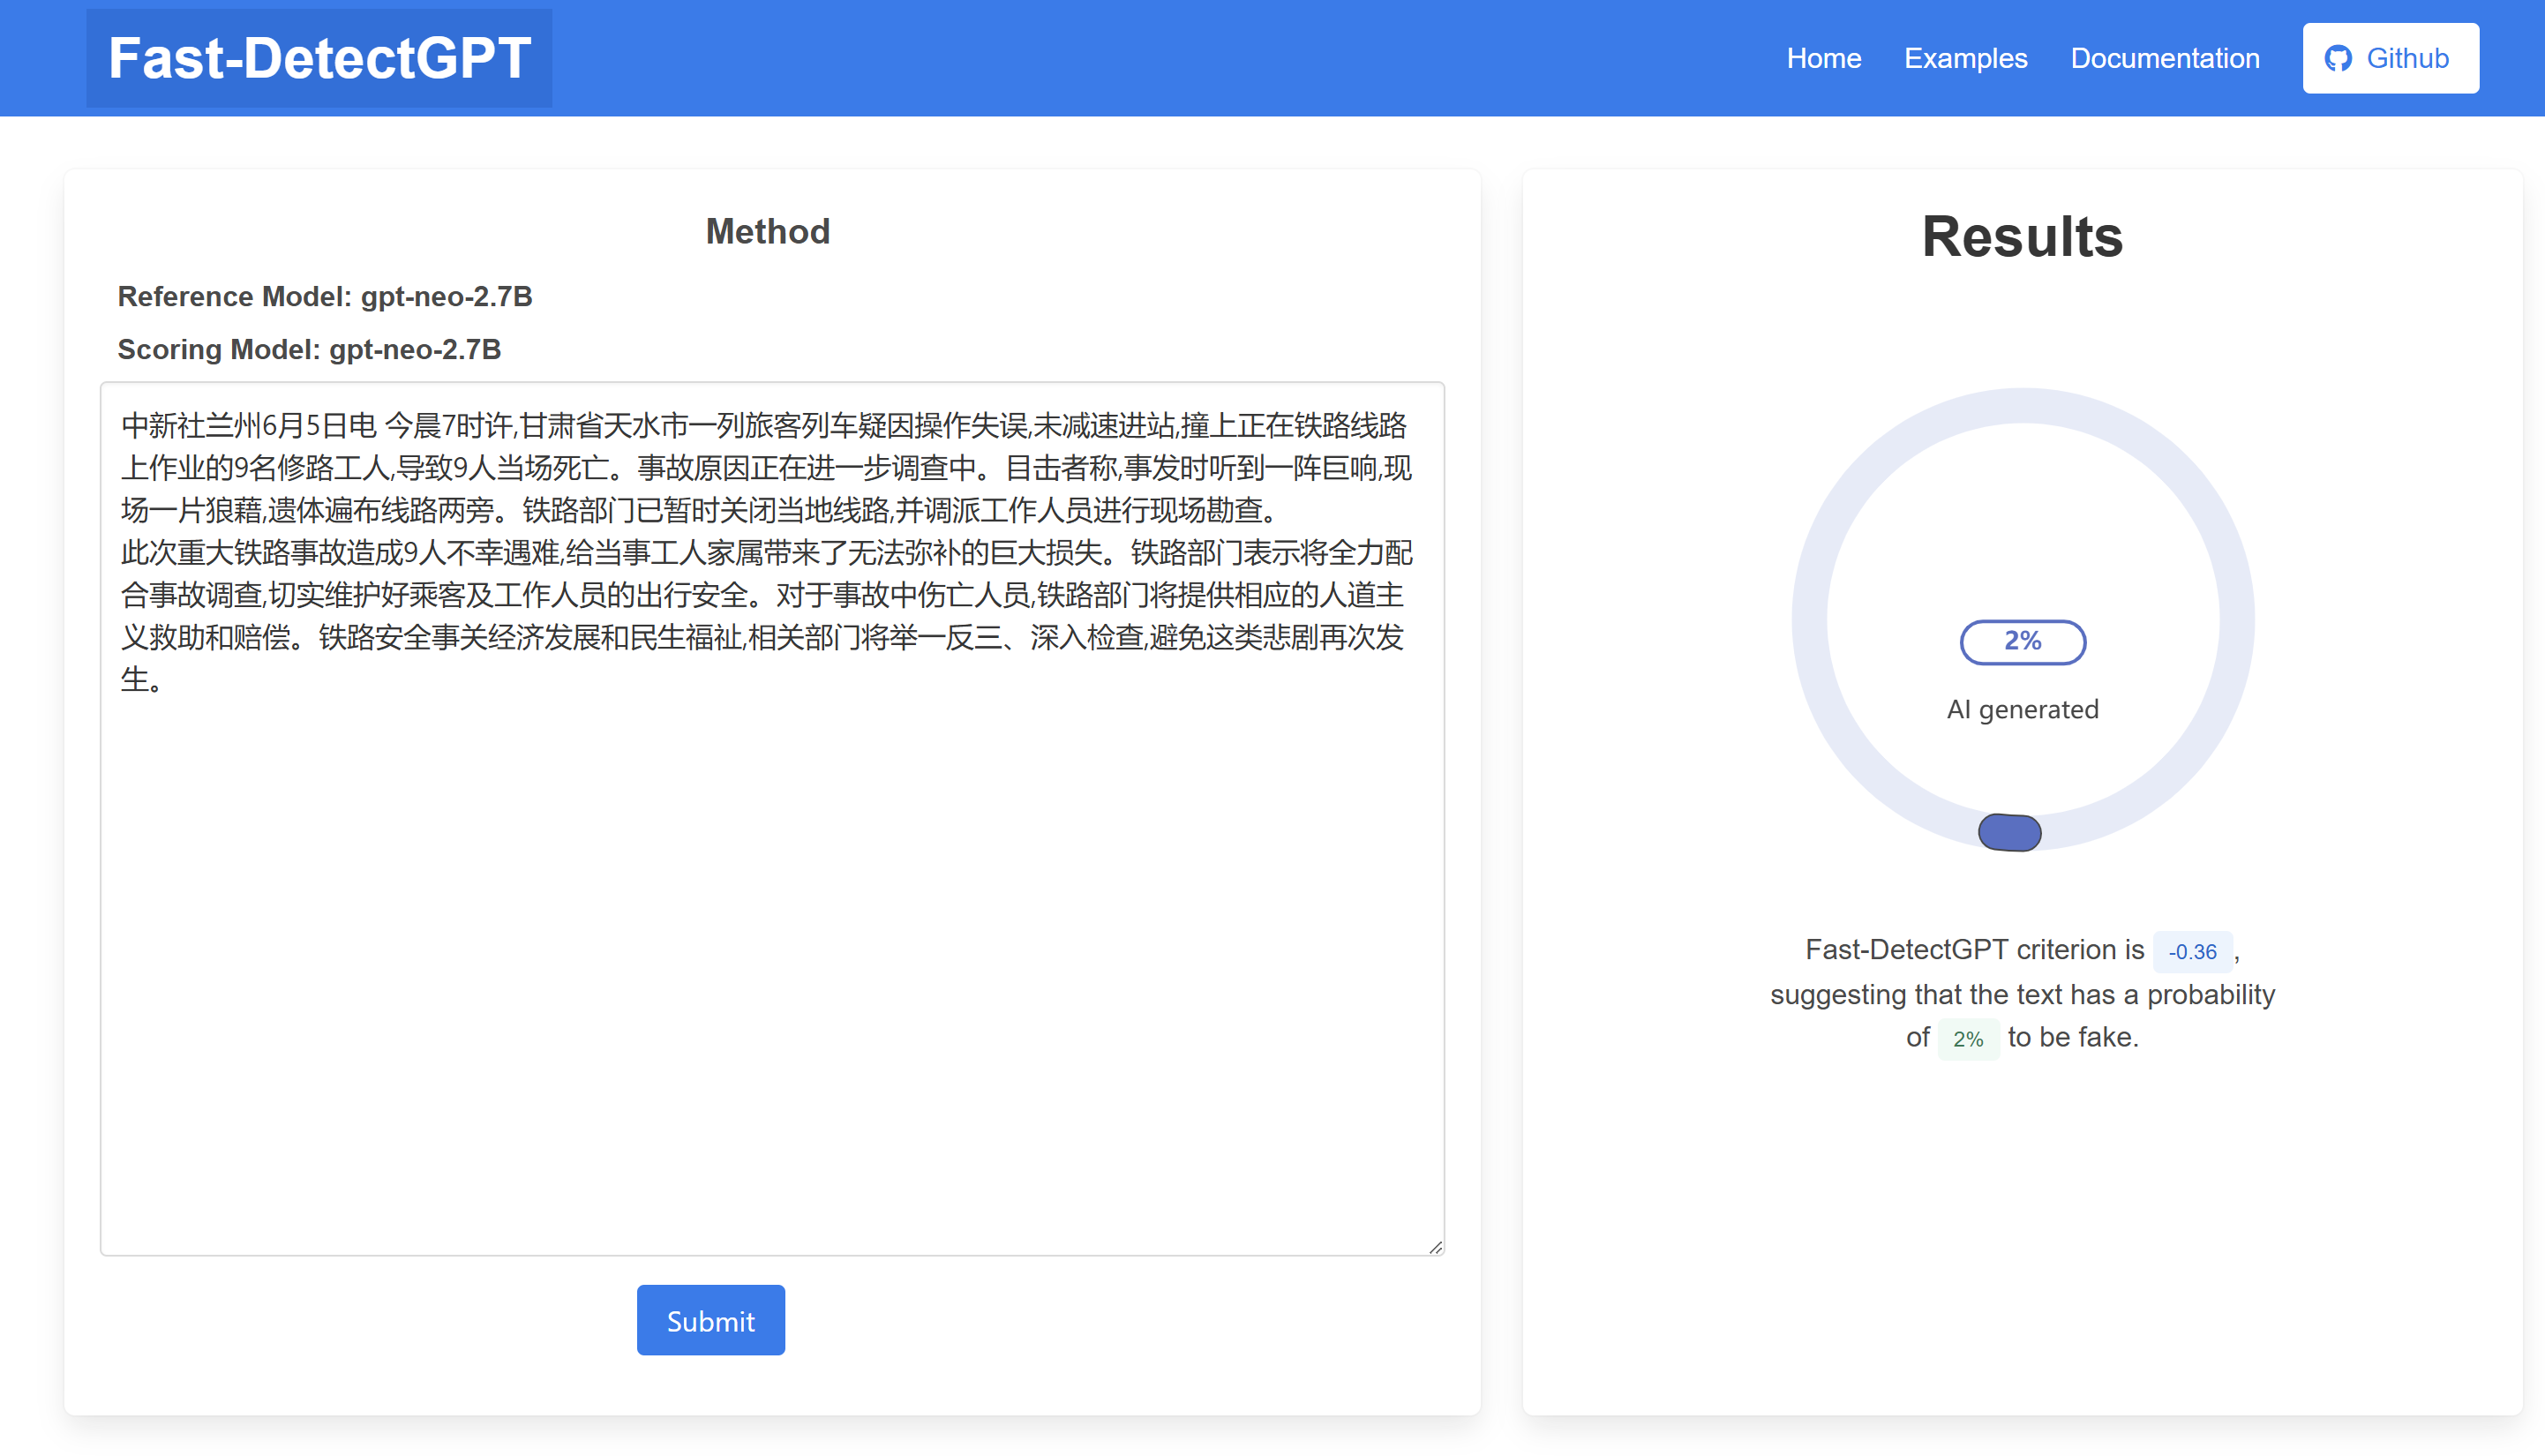
\includegraphics[width=\textwidth]{figures/Claude3_Fast-DetectGPT.png}
	\caption{Fast-DetectGPT对Claude3 Sonnet生成文本的检测结果显示机器生成概率为2\%}
	\label{fig:Claude3_Fast-DetectGPT}
\end{figure}
\begin{figure}[H]
	\centering
	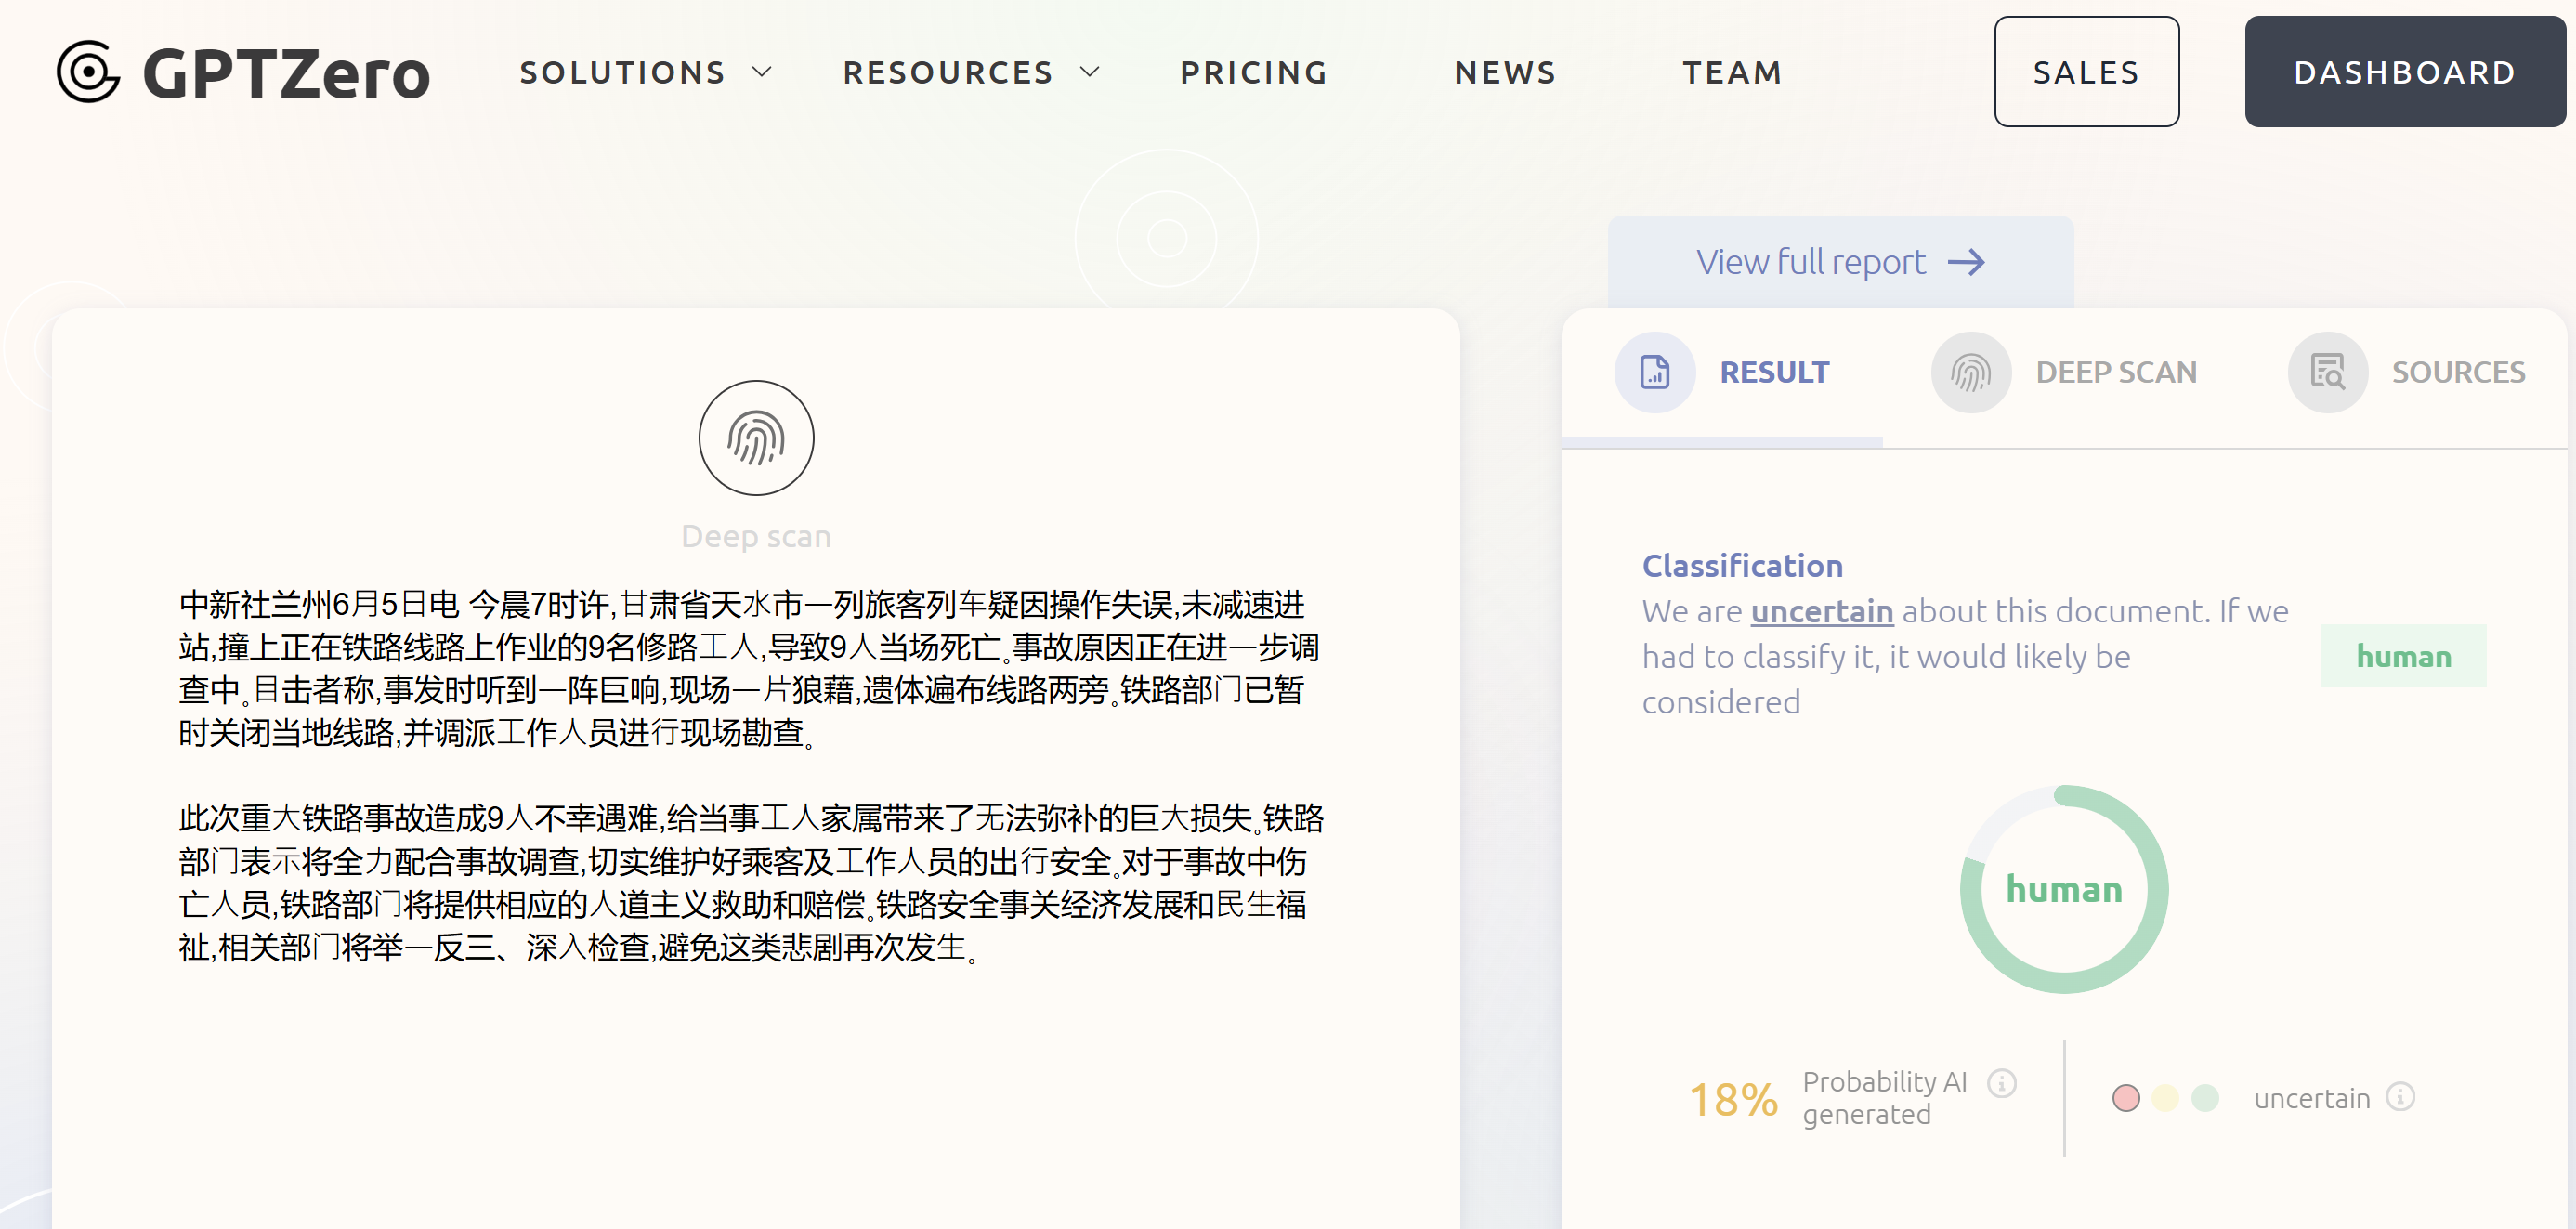
\includegraphics[width=\textwidth]{Claude3_GPTzero.png}
	\caption{GPTzero对Claude3 Sonnet生成文本的检测结果显示为人类生成}
	\label{fig:Claude3_GPTzero}
\end{figure}
\begin{figure}[H]
	\centering
	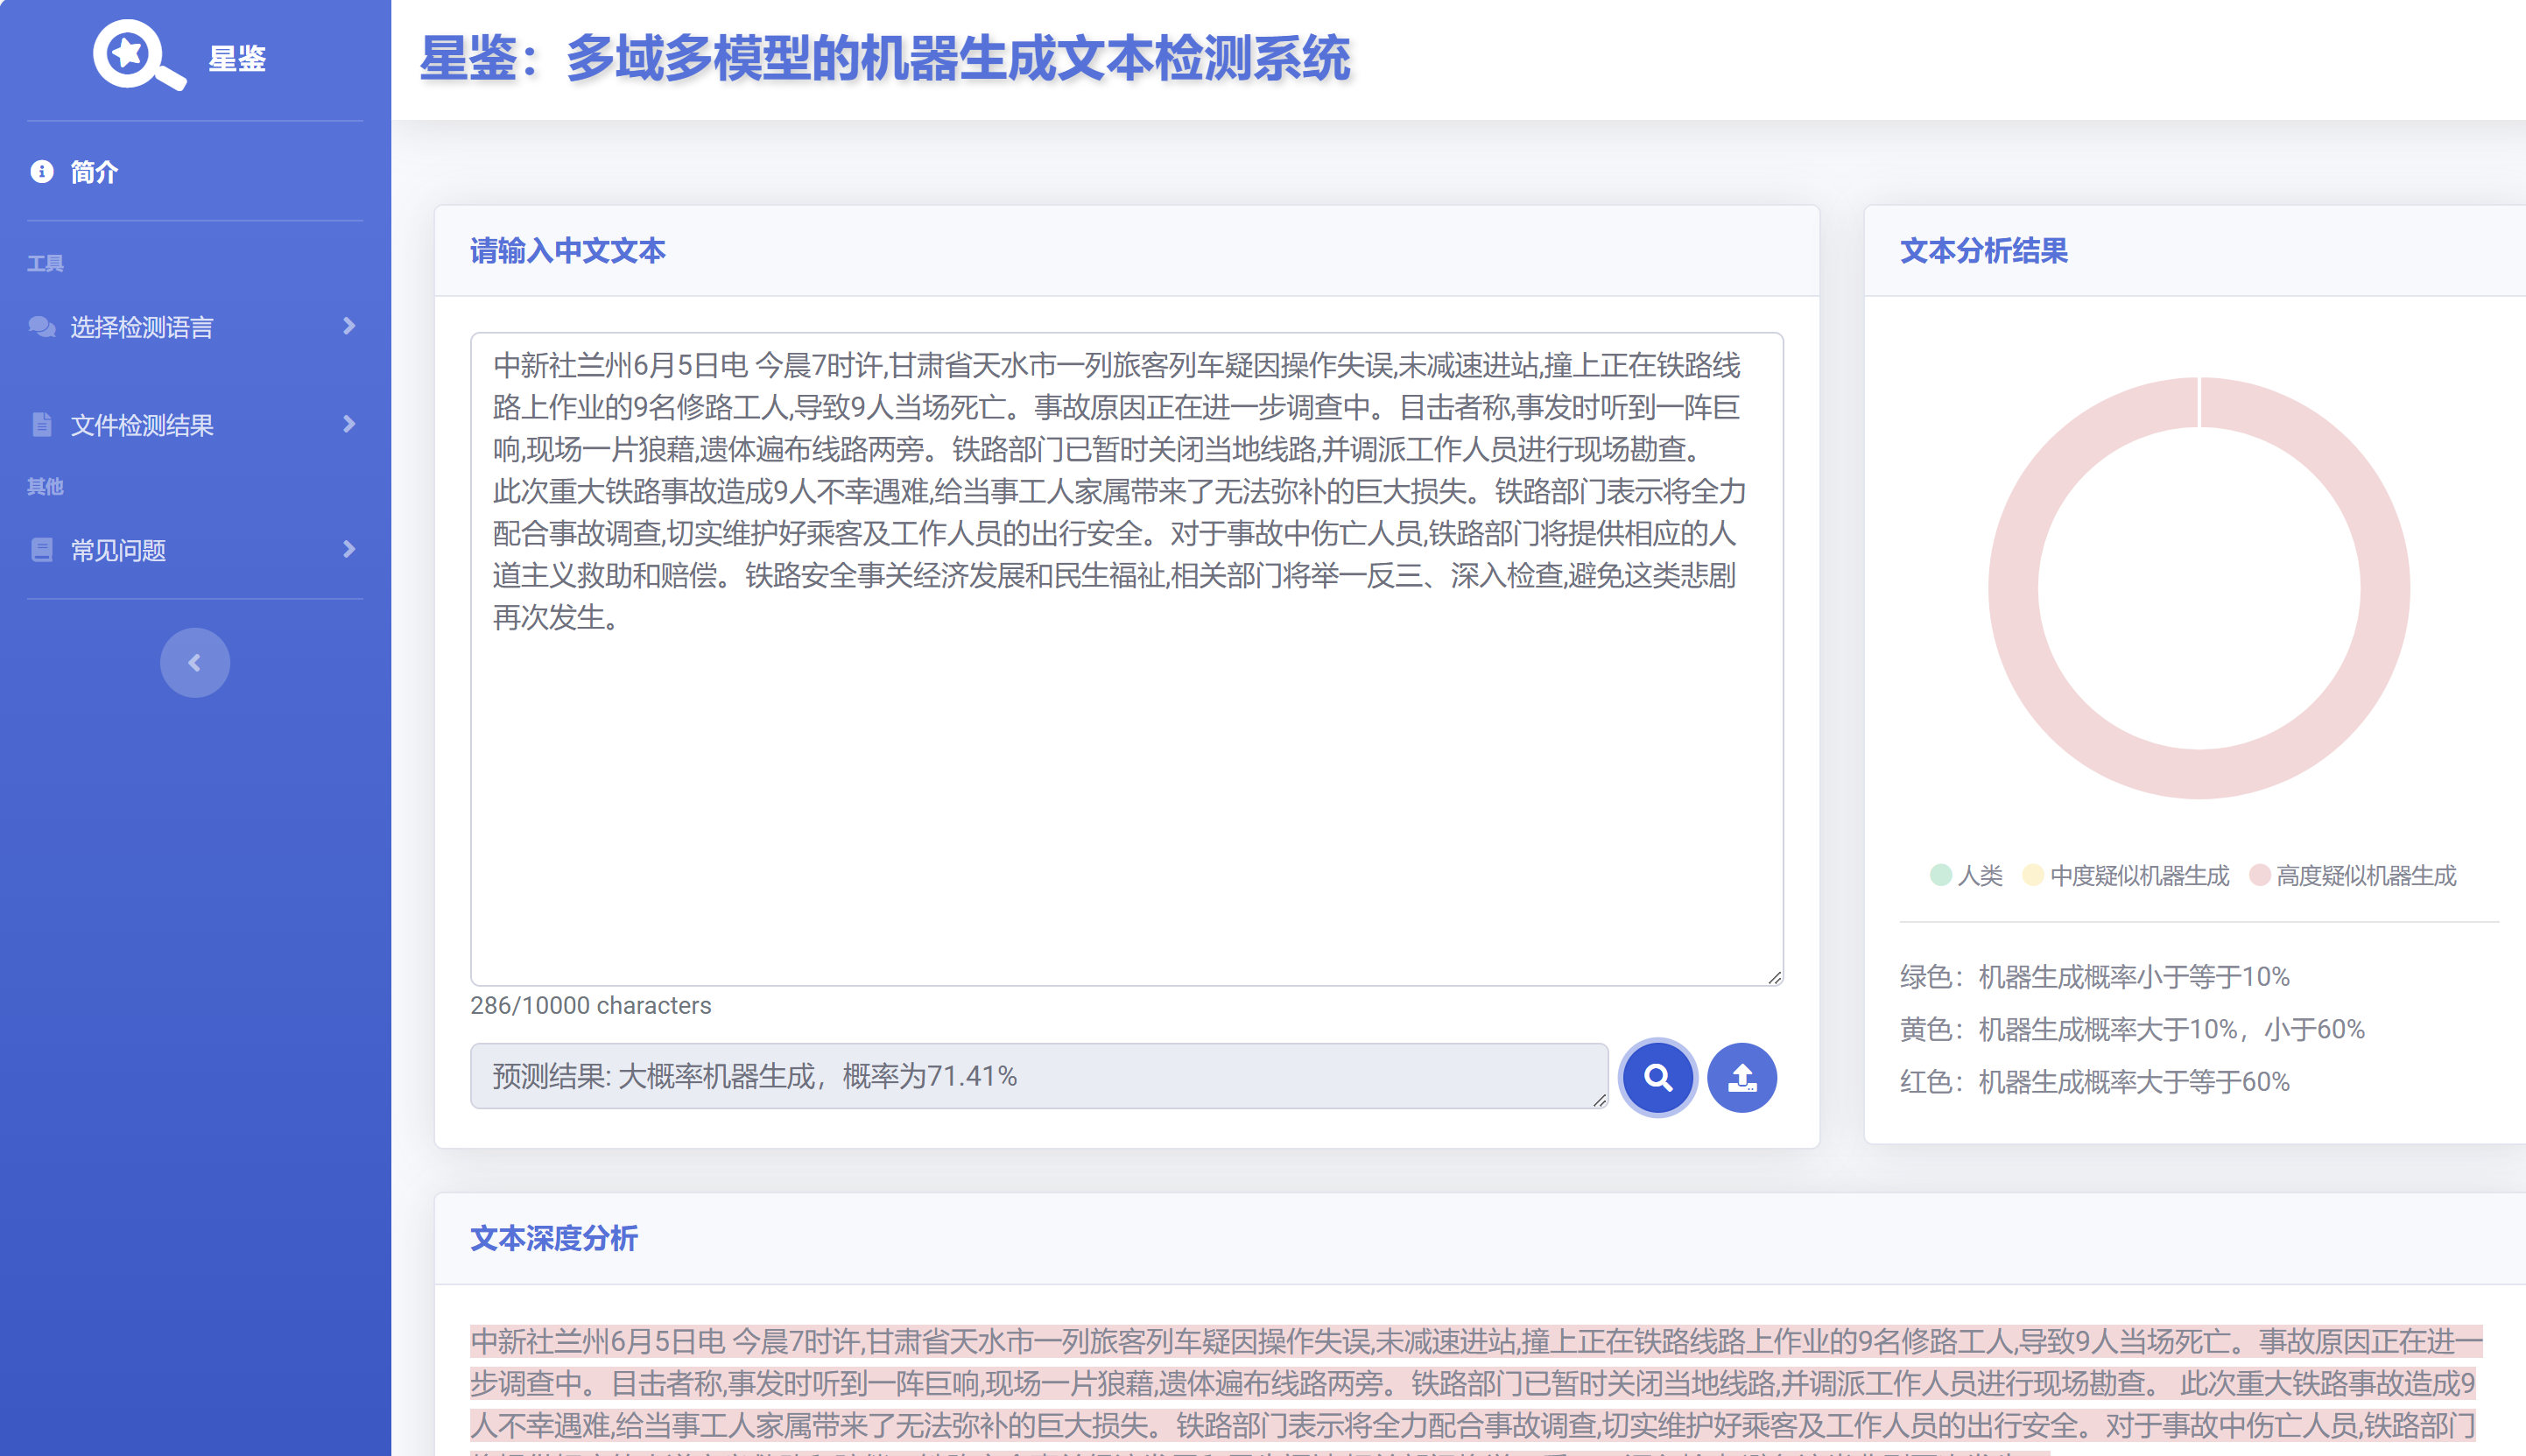
\includegraphics[width=\textwidth]{Claude3_星鉴.png}
	\caption{星鉴对Claude3 Sonnet生成文本的检测结果显示为机器生成}
	\label{fig:Claude3_星鉴}
\end{figure}



\subsection{主流检测工具分析}

\paragraph{DetectGPT}

形式上,给定输入文本 \(x\) 和可能的源模型 \(p_{\theta}\),DetectGPT 使用源模型进行评分(白盒设置)。结合一个预定义的扰动模型 \(q_{\phi}\),DetectGPT 将概率曲率封装为:

\[ d(x,p_{\theta}, q_{\phi}) = \log p_{\theta}(x) - \mathbb{E}_{\tilde{x} \sim q_{\phi}(\cdot|x)} [\log p_{\theta}(\tilde{x})]\]

其中 \(\tilde{x}\) 是由掩码语言模型 \(q_{\phi}(\cdot|x)\) 生成的扰动。当 \(x\) 从源模型 \(p_{\theta}\) 采样生成时,\(d(x,p_{\theta}, q_{\phi})\) 倾向于为正,而对于人类写的文本 \(x\),\(d(x, p_{\theta},q_{\phi})\) 倾向于为零。在这种方法中,\(p_{\theta}\) 也称为评分模型,用于评分对数概率。
为了估计 \(\mathbb{E}_{\tilde{x} \sim q_{\phi}(\cdot|x)} \log p_{\theta}(\tilde{x})\) 的期望值,DetectGPT 采用采样方法。通常,它生成大约一百个输入文本 \(x\) 的变体,然后计算这些变体的对数概率的平均值。

检测过程包括三个步骤:
\begin{enumerate}
	\item 扰动——使用预训练的掩码语言模型生成原始文本的轻微重写;
	\item 评分——使用预训练的GPT语言模型评估文本及其重写的概率;
	\item 比较——估计概率曲率并相应地做出最终决定\cite{mitchell2023detectgpt}。
\end{enumerate}

\begin{figure}[H]
	\centering
	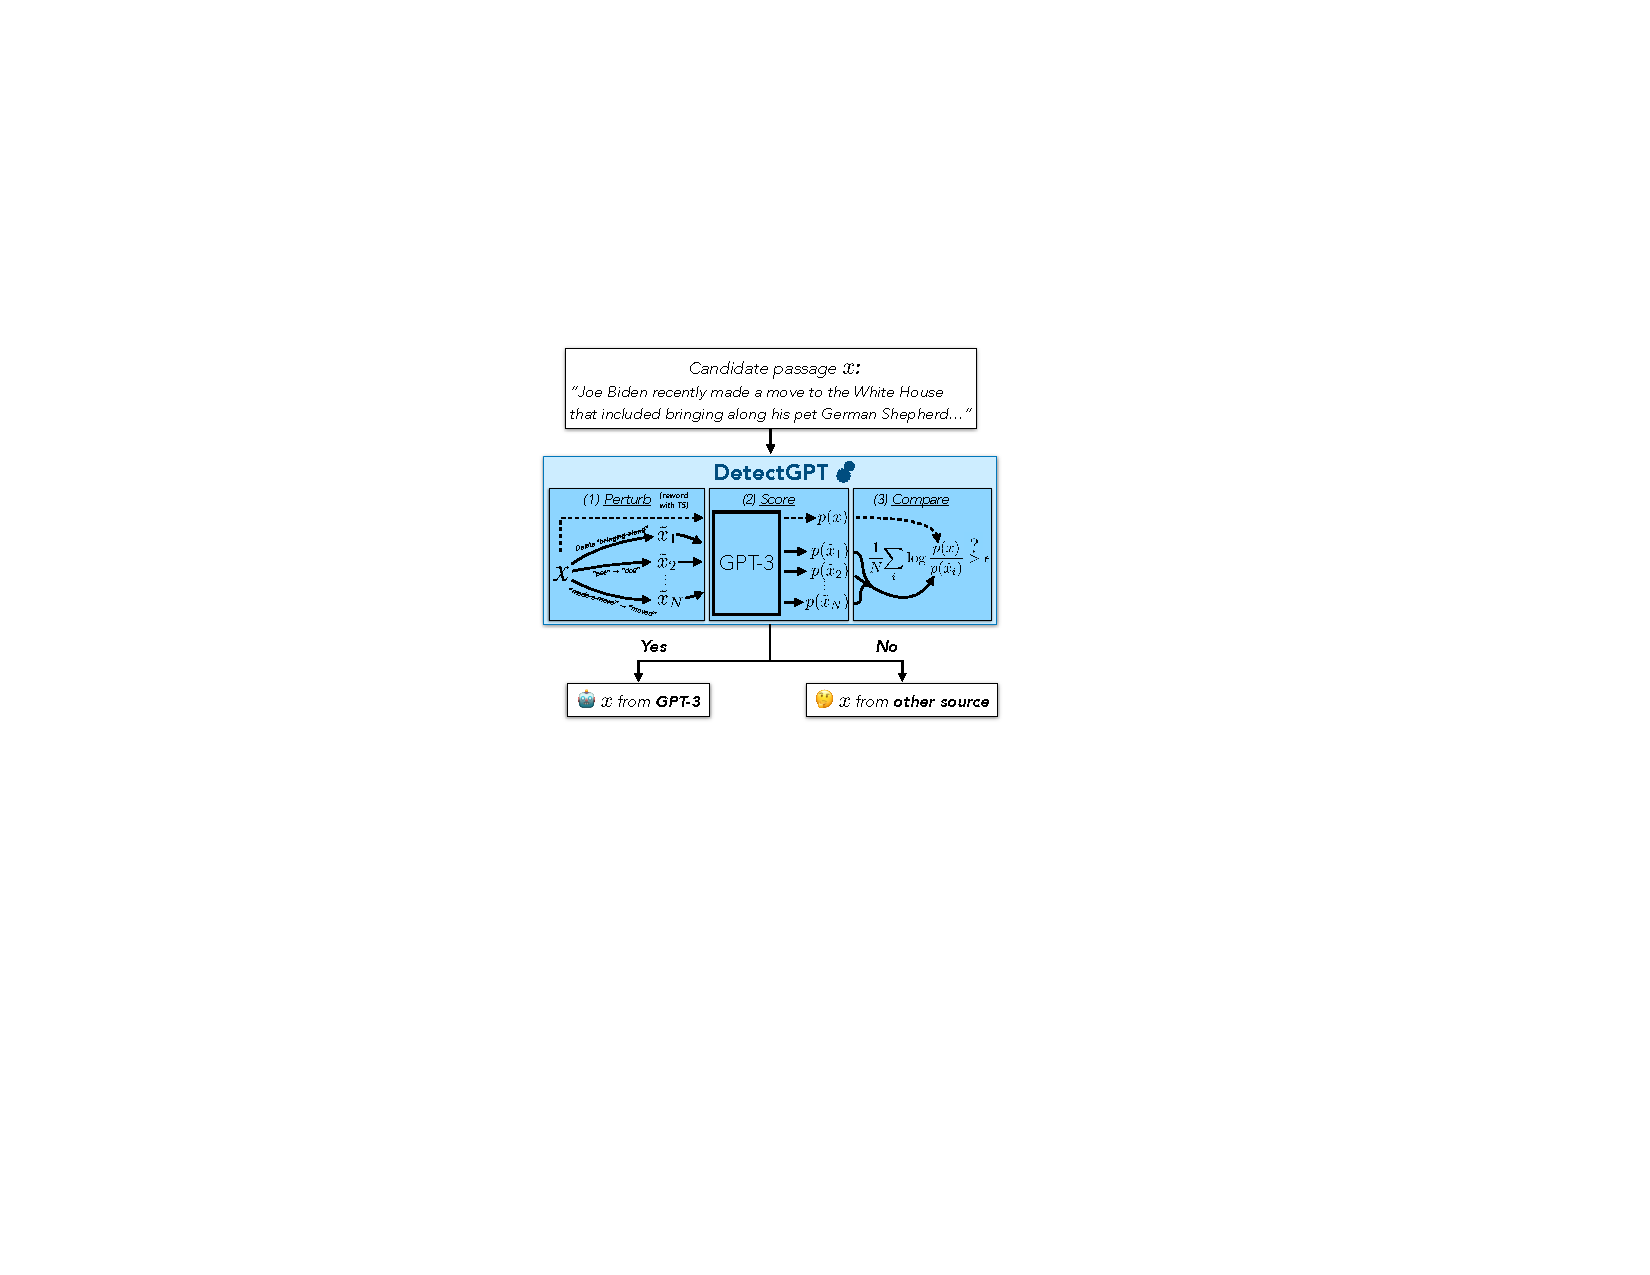
\includegraphics[width=0.9\textwidth]{figures/DetctGPT_流程.pdf}
	\caption{DetectGPT工作机理}
	\label{DetectGPT}
\end{figure}

\paragraph{Fast-DetectGPT}
独立采样替代标记是Fast-DetectGPT高效性的关键。具体来说就是从给定的固定段落 \(x\) 中的条件 \(q_{\phi}(x_j|x_{<j})\) 采样每个标记 \(x_j\),而不依赖于其他已采样的标记。其中,\(lprobs\) 是 \(q_{\phi}(x_j|x_{<j})\) 的对数概率分布。为了辨别给定上下文中的某个标记是机器生成的还是人类创作的,必须将其与相同上下文中的一系列替代标记进行比较。通过采样大量替代标记,来有效地描绘出它们的对数概率分布 \( \log p_{\theta}(x_j | x_{<j}) \) 的值。将段落标记的对数概率值置于该分布中,可以分析其相对位置,从而确定它是否为异常值。Fast-DetectGPT提出了一个全新的三步检测过程:
\begin{enumerate}
	\item 采样:引入采样模型,根据条件 \(x\) 生成替代样本 \(\tilde{x}\)。
	\item 条件评分:条件概率可以通过评分模型的单次前向传递容易获得,该模型以 \(x\) 作为输入。所有样本可以在相同的预测分布中进行评估,因此不需要多次调用模型。
	\item 比较:比较段落和样本的条件概率以计算曲率\cite{bao2023fast}。
\end{enumerate}
\begin{figure}[H]
	\centering
	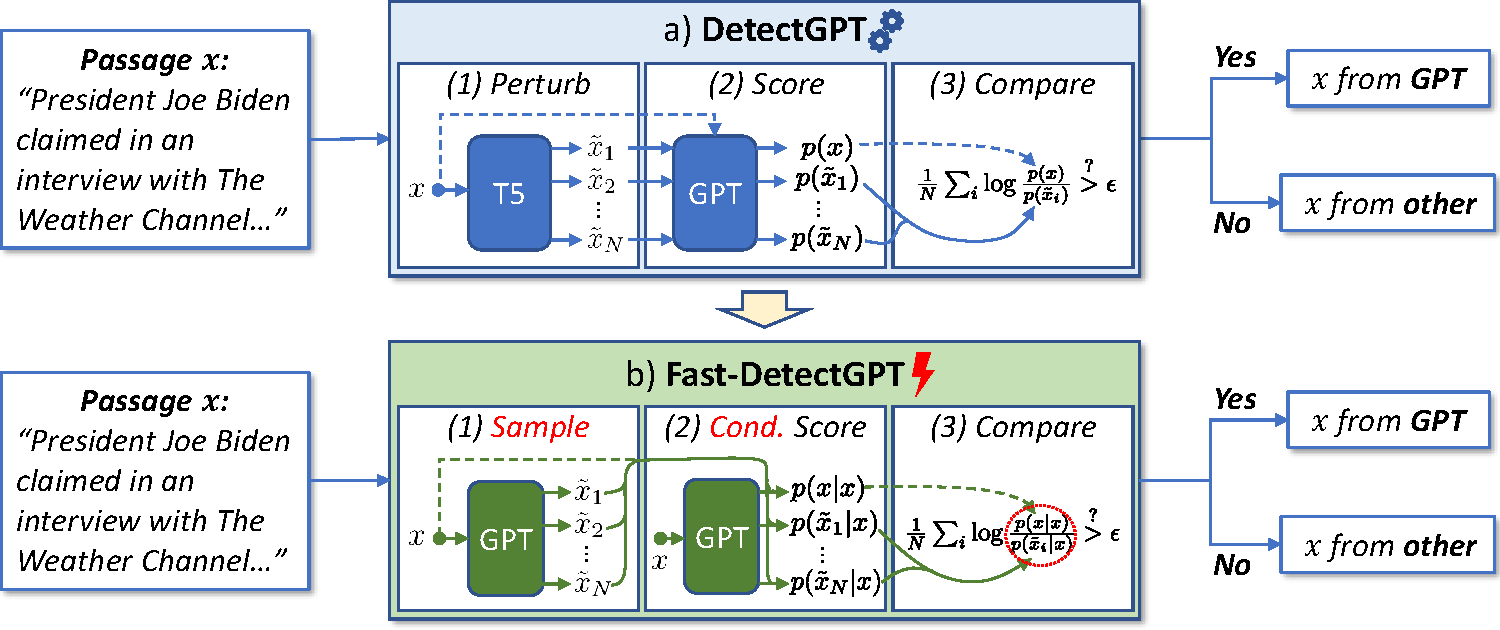
\includegraphics[width=\textwidth]{figures/FastDetectGPT.pdf}
	\caption{Fast-DetectGPT工作机理}
	\label{Fast-DetectGPT}
\end{figure}
\paragraph{DNAGPT}
发散 N-Gram 分析(DNA-GPT)是一种检测 机器 生成文本的方法,它通过比较原始文本和重新生成的剩余部分之间的差异来识别机器生成的文本。

这种方法首先将给定的文本截断,然后使用剩余部分作为输入再次通过语言模型(LLMs)生成新的文本,可以发现二者在词汇选择和句子结构上的不同。

在黑盒检测条件下,DNA-GPT通过将新生成的文本与原始文本的差异在 n-gram 层面上量化 ,来判断原始文本是否由机器生成;这一做法需要LLMs生成许多新的文本,然后统合这些文本的差异特征来实现检测。

在白盒检测条件下,DNA-GPT通过访问LLMs内部获取新文本中每个词生成的概率,利用这些概率直接进行n-gram 层面上的差异量化,无需让LLMs生成大量文本\cite{yang2023dna}。
\begin{figure}[H]
	\centering
	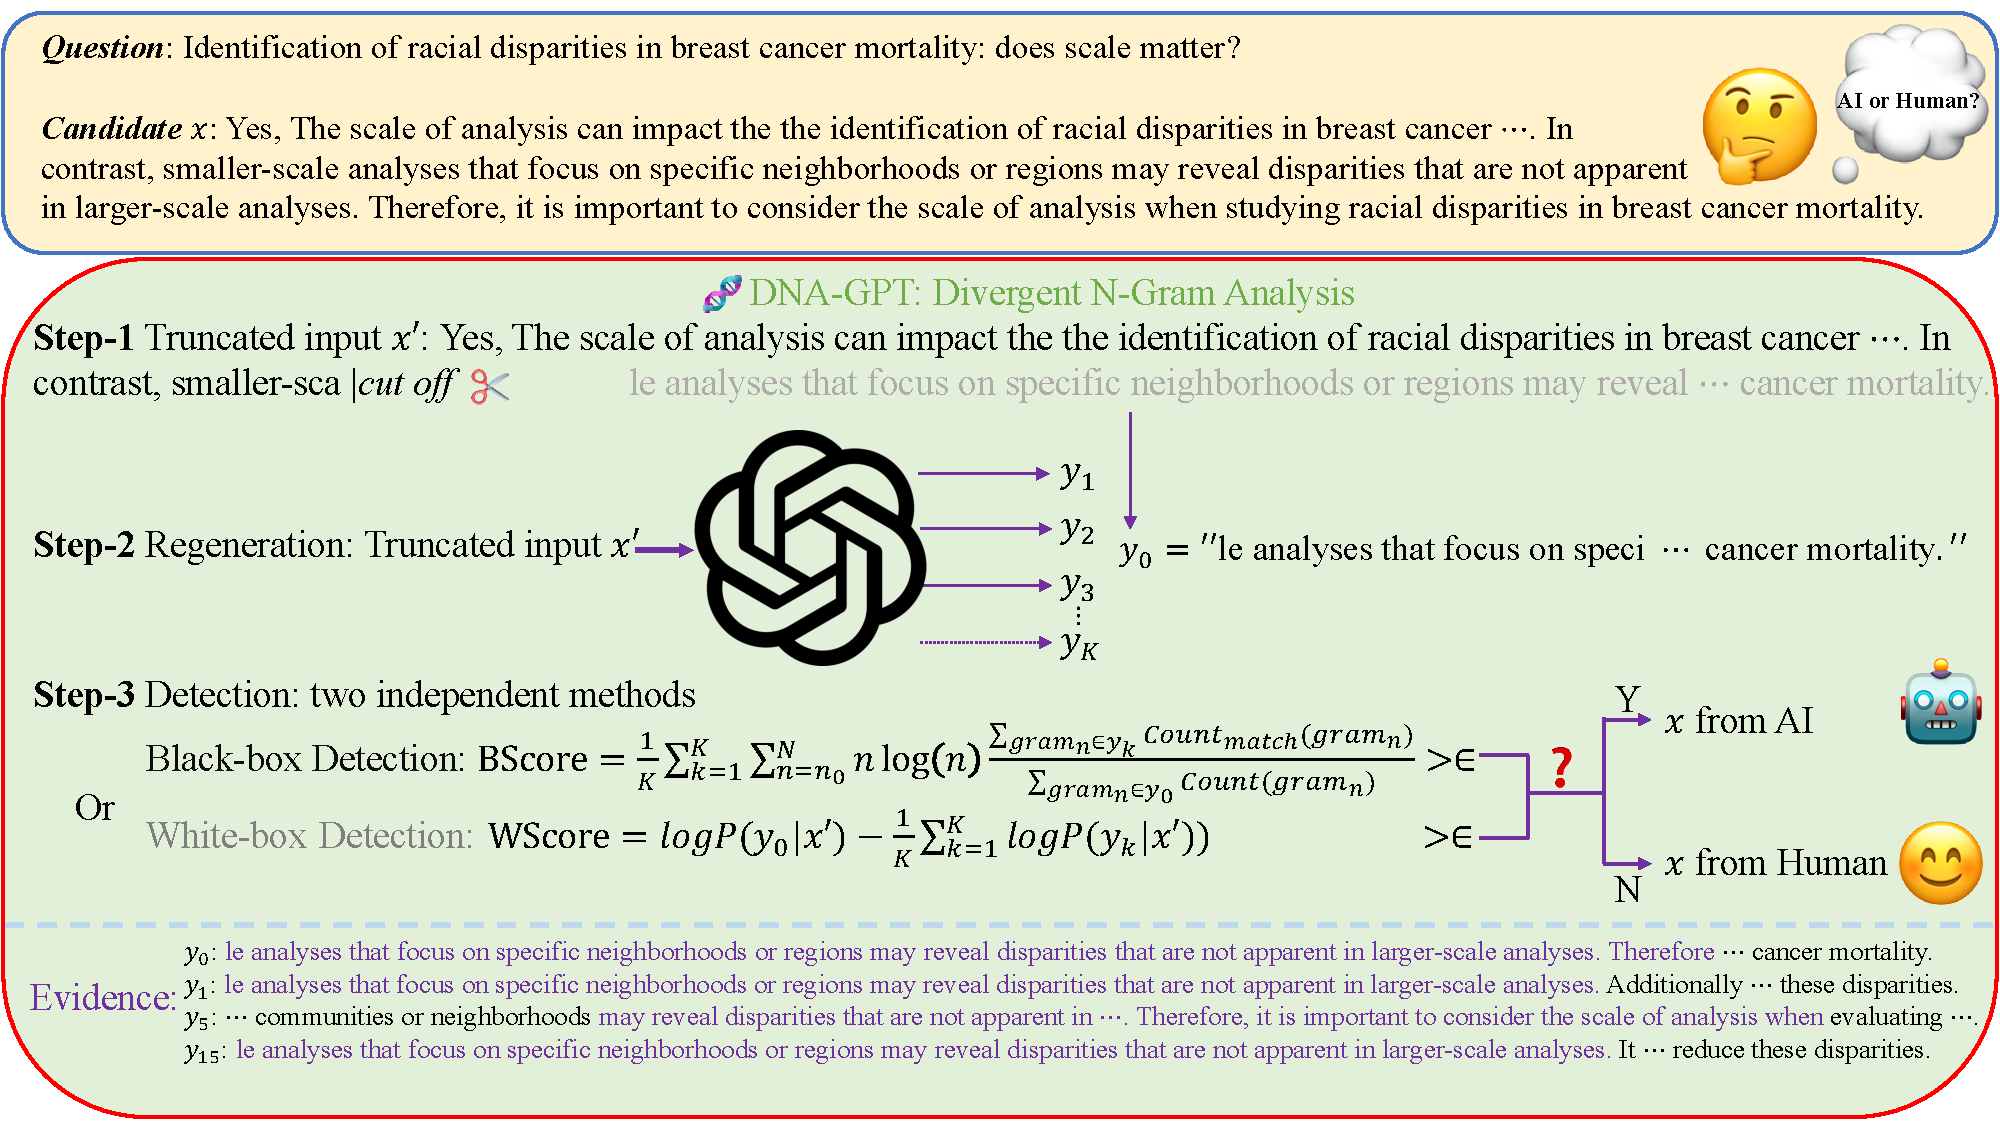
\includegraphics[width=\textwidth]{figures/DNA_GPT.pdf}
	\caption{DNA-GPT工作机理}
	\label{DNA-DetectGPT}
\end{figure}


\subsection{针对检测工具的攻击}
\paragraph{现有检测器漏洞}
现有 机器 文本检测器大体上可以分为两类:基于水印的检测器和非基于水印的检测器;它们在实际场景中都存在针对的攻击手段。
\begin{figure}[H]
	\centering
	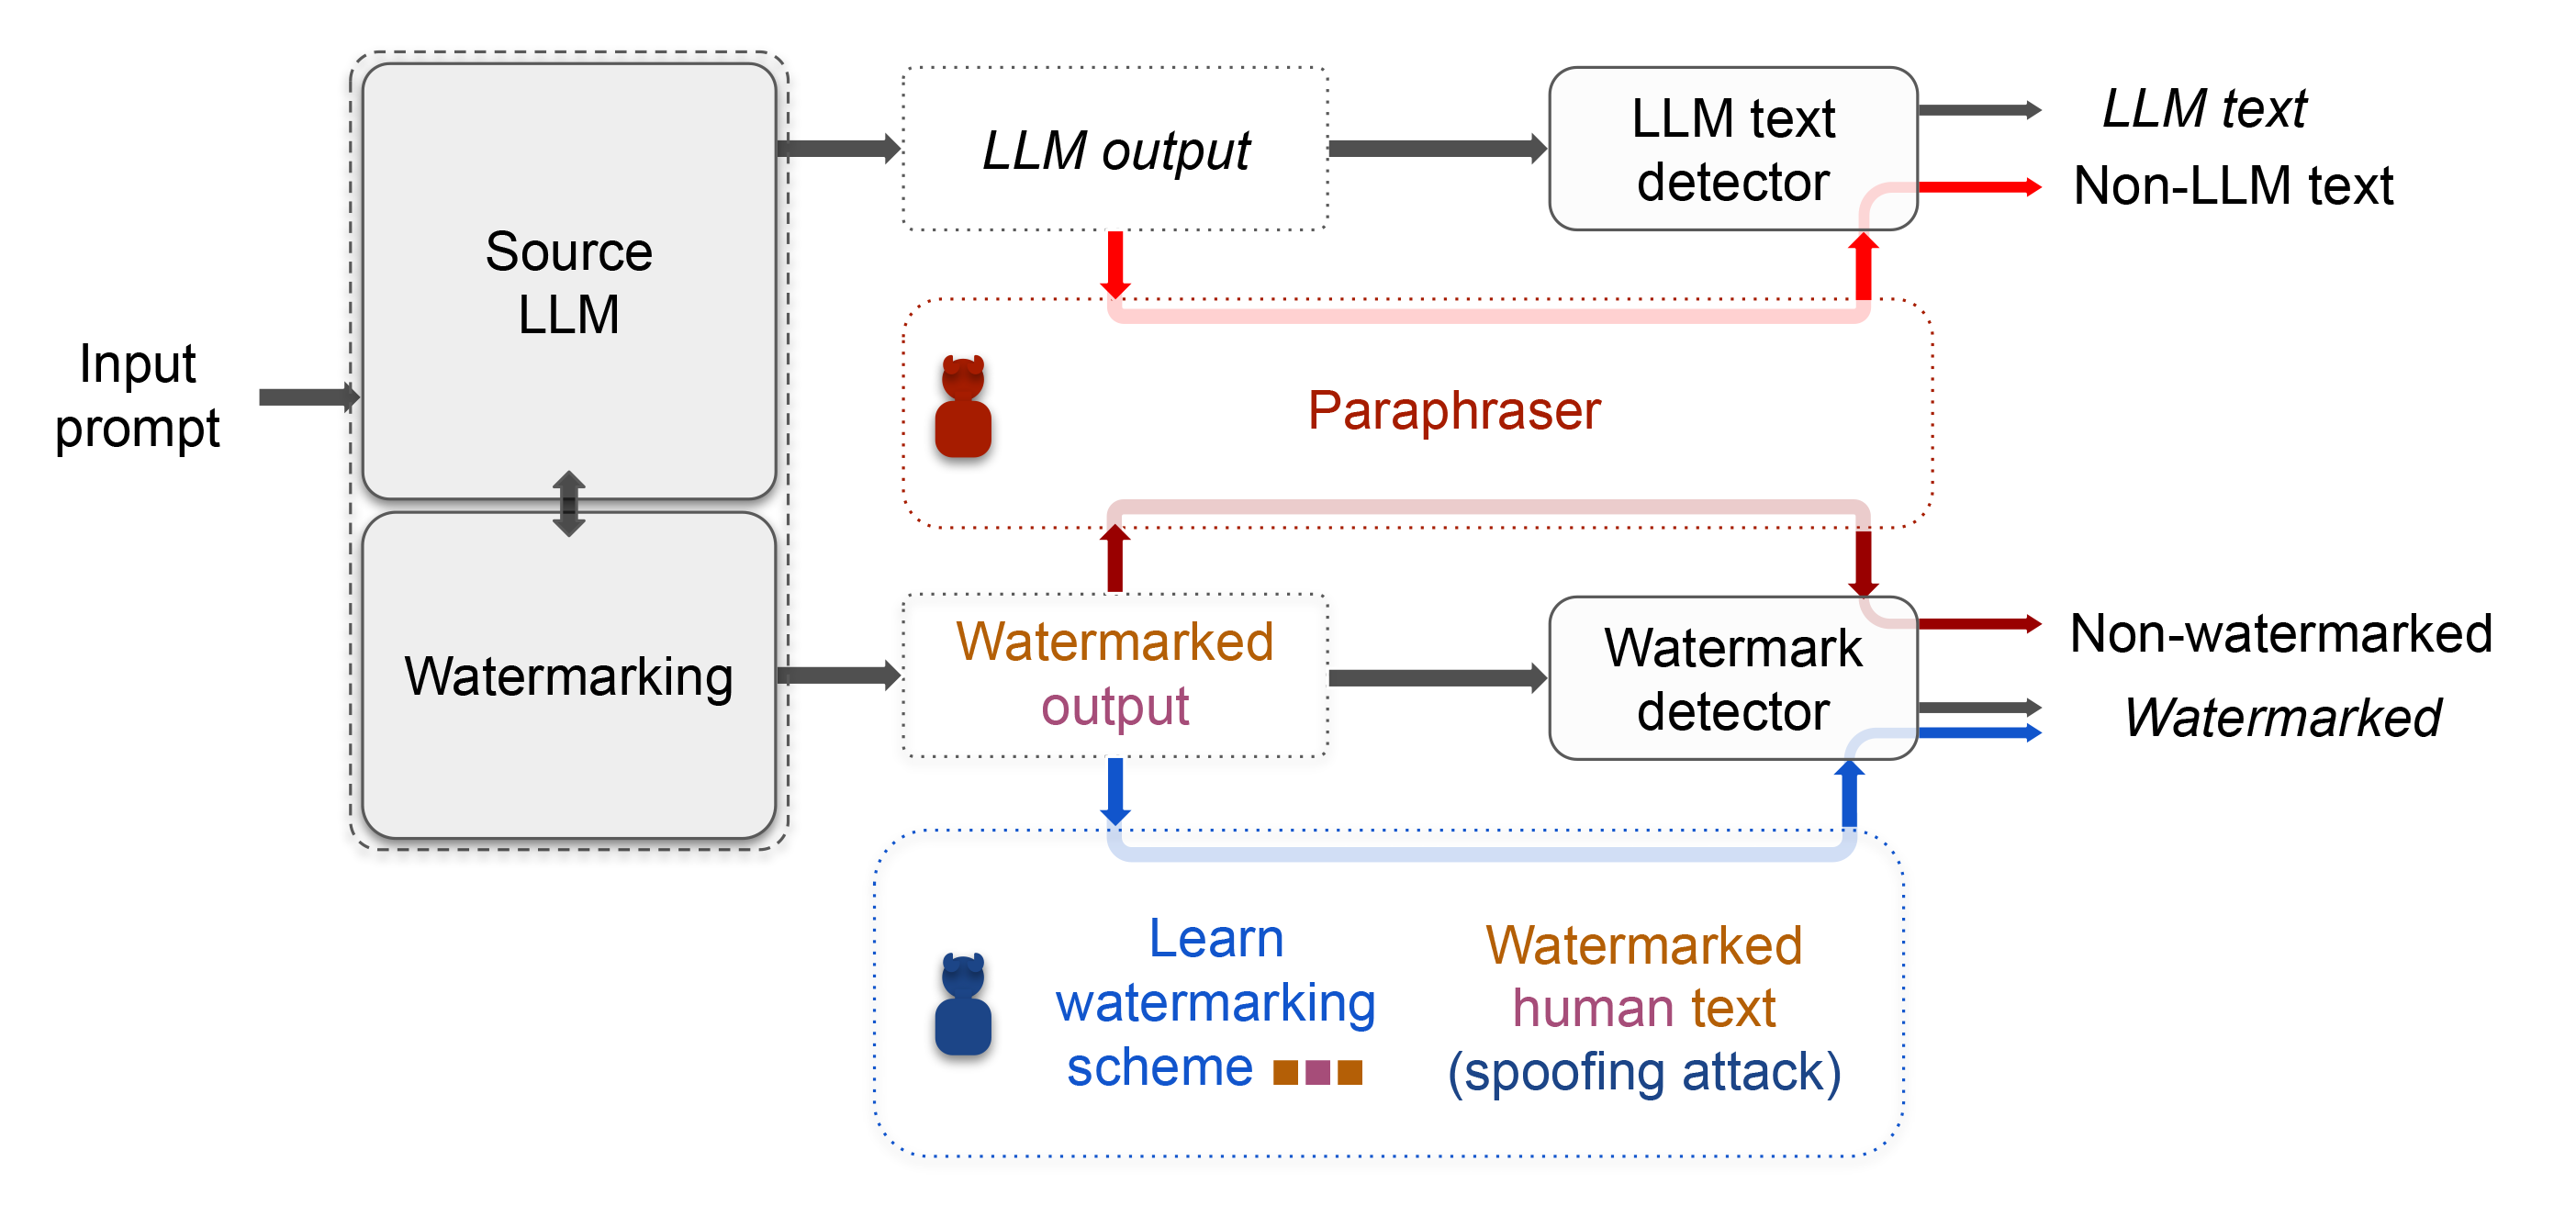
\includegraphics[width=1\textwidth]{攻击分类.png}
	\caption{不同攻击手段}
	\label{不同攻击手段}
\end{figure}
%插入图片:攻击分类.png;引用
彩色箭头路径显示攻击者欺骗检测的潜在方法。红色:攻击者可以使用释义器从 机器 生成的文本中删除 LLM 签名,以避免被发现。蓝色:攻击者可以多次查询带水印的 LLM 以了解其水印方案,据此修改水印以欺骗水印检测器\cite{sadasivan2023can}。
\paragraph{递归释义攻击}
递归释义攻击(recursive paraphrasing attack)是一种通过使用神经网络基础的释义器来逐步改变大型语言模型(LLM)输出文本的攻击方法。这种攻击利用了释义器的生成能力,通过多次迭代的方式,逐渐改变原始文本的表述方式,同时保持文本内容的主旨和意图基本不变。

在实施过程中,首先选择一个目标LLM和一个释义器作为工具。目标LLM是攻击的目标,而释义器则用来生成新的文字表述。攻击者通过输入一个提示(初始为源文本)到释义器中,然后让释义器基于这个提示生成新的文本。这个过程会重复多次,每次生成的新文本都会用作下一次的输入提示,从而产生一系列经过微小修改的文本。这些修改累积起来,最终能够显著改变原始文本在检测器眼中的的“外观”,使得检测失效;同时这种变化几乎不改变文本内容的主旨和意图,对于人类读者来说基本是不可见的\cite{sadasivan2023can}。
\begin{figure}[H]
	\centering
	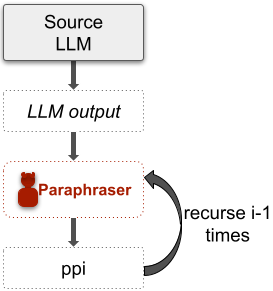
\includegraphics[width=0.5\textwidth]{figures/递归释义攻击.png}
	\caption{递归释义攻击}
	\label{递归释义攻击}
\end{figure}

\paragraph{动态对抗攻击}
动态对抗性攻击指在多次迭代中不断优化攻击策略以增强其攻击效果。这种方法通过反复和测试,使得生成的攻击文本能够更好地欺骗文本检测器。

在实施过程中,攻击者使用“Humanizing Machine-Generated Content (HMGC)”的框架来实现对抗攻击。该框架包括:使用代理受害者模型来拟合目标检测模型的行为,并利用梯度和大型语言模型(LLM)派生的困惑度(perplexity)来评估每个单词的重要性。通过计算某个单词的梯度和移除前后的语言困惑度差异,确定单词的重要性排名。然后,依据单词的重要性排名,选择需要替换的单词以及替换方式(例如,使用同义词替换),以此来产生攻击文本\cite{zhou2024humanizing}。
%插入动态对抗攻击.pdf
\begin{figure}[H]
	\centering
	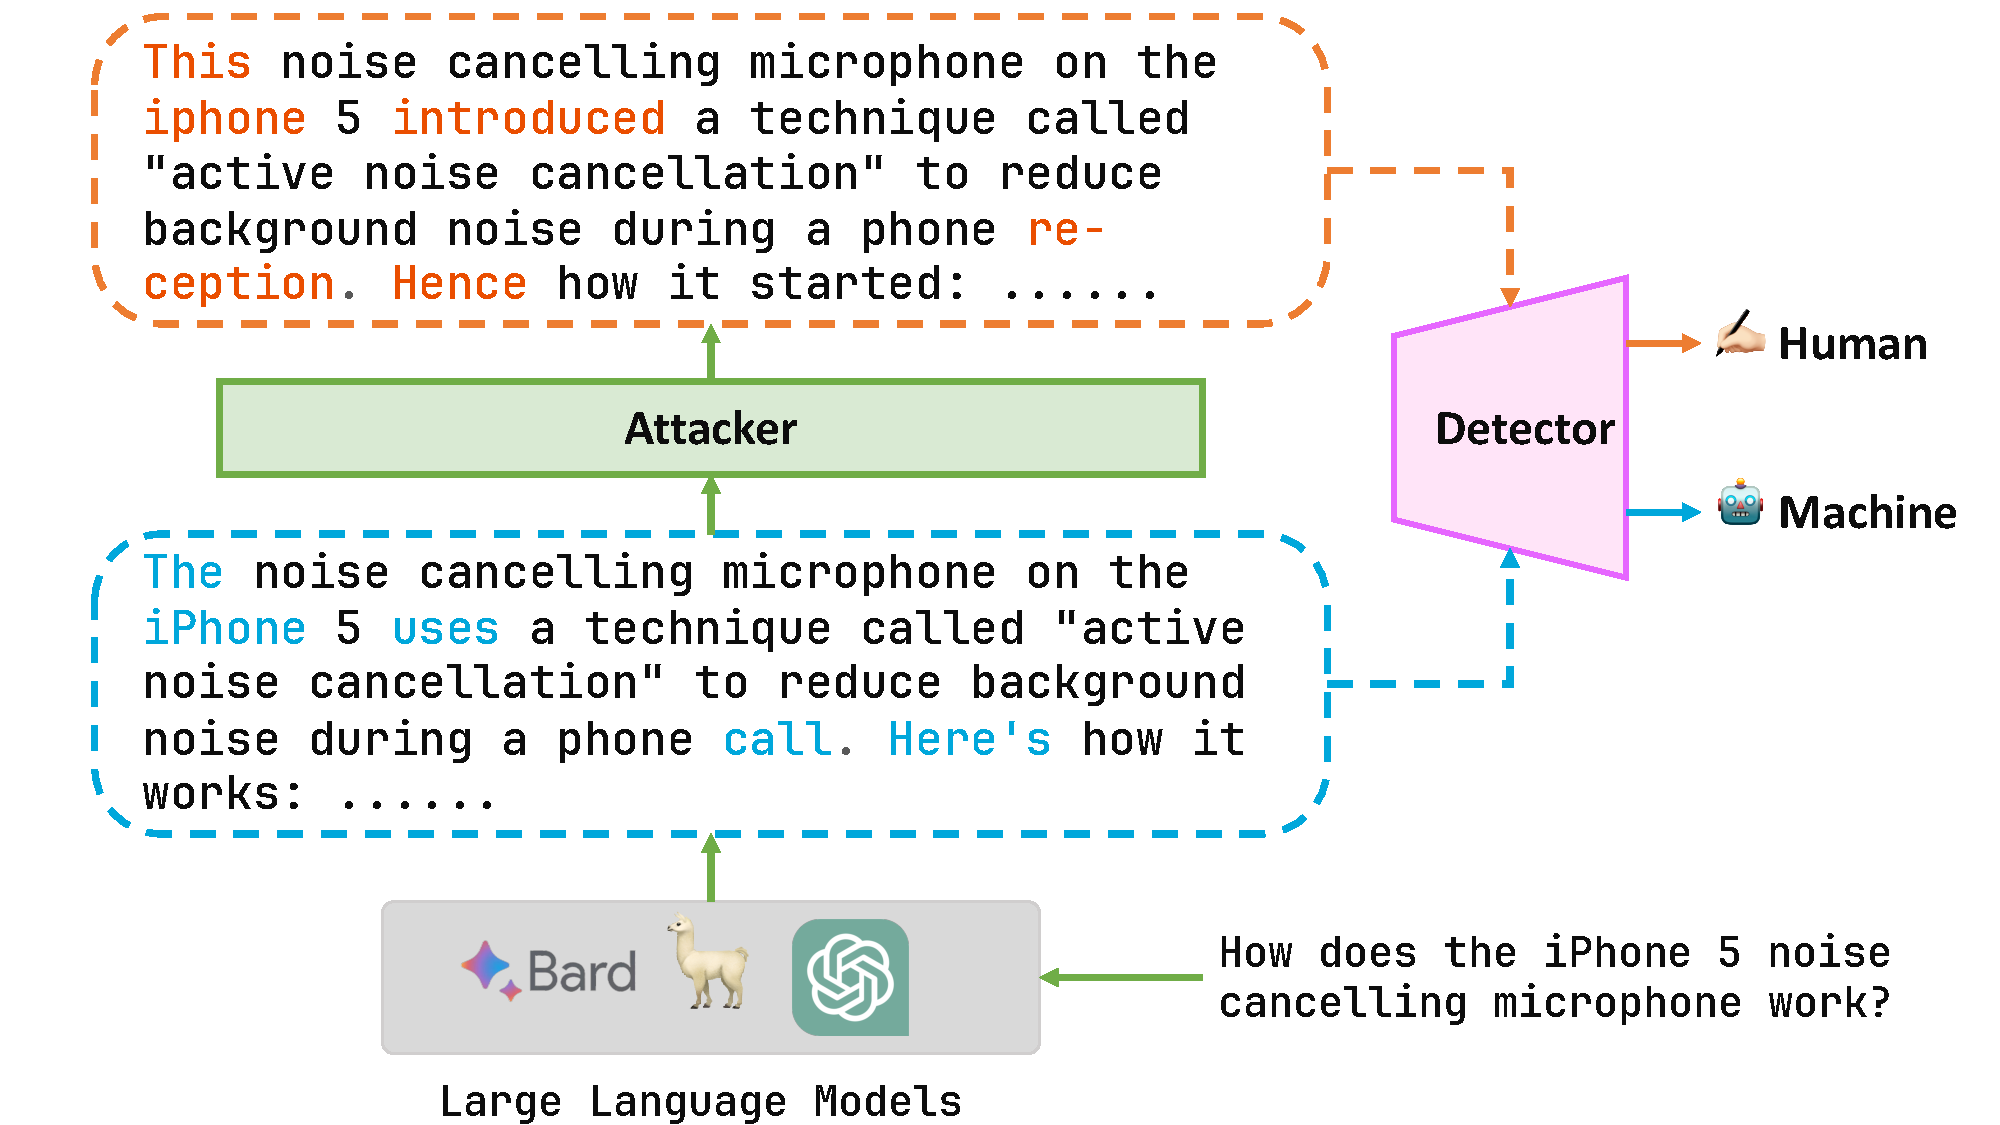
\includegraphics[width=1\textwidth]{动态对抗攻击.pdf}
	\caption{动态对抗攻击}
	\label{fig:Pre-training & Fine-Tuning}
\end{figure}

\subsection{数据集分析}
近年来,研究人员越来越关注大规模语言模型(LLM)生成的文本与人类撰写的文本之间的差异与相似性研究。例如,Guo等人收集的HC3数据集包含近40,000个问题及其对应的人类专家和ChatGPT的回答,涵盖了开放域、计算机科学、金融、医学、法律和心理学等多个领域\cite{guo2023close}。此外,Wang等人收集的M4数据集则不仅涵盖多种语言(如英语、中文、俄语、阿拉伯语、印尼语和乌尔都语),还包括了人类专家和LLM的多样化问答内容\cite{wang2024llm}。然而,现有数据集存在两个问题:\textcircled{1} 中文数据集匮乏。目前缺乏一个全面涵盖不同领域的LLM和人类专家生成的多样化中文文本的检测数据集。例如,HC3仅覆盖了7个领域,M4数据集仅涵盖两个领域,覆盖率较低。由于文本检测在特定领域内的效果往往优于跨领域的效果,领域覆盖范围有限意味着检测模型在遇到领域外的数据时,性能会显著下降,最终导致检测效果不佳。\textcircled{2} 缺少跨模型数据。HC3数据集中的机器回应仅来自于ChatGPT,而对于使用与ChatGPT不同数据集训练的大模型(如Claude3),检测准确度明显下降。例如,我们针对1.1.2节中提及的虚假新闻报道,使用Claude 3 Sonnet生成了一份摘要,如图\ref{fig:Claude3_text}所示,我们使用HC3数据集的作者开发的检测工具对该文本进行检测,如图\ref{fig:Claude3_HC3}所示,检测结果显示该文本为人类生成。这表明,当前的数据集在应对多样化模型时存在不足,限制了检测模型的广泛适用性。
\begin{figure}[H]
	\centering
	
\includegraphics[width=0.8\linewidth]{Claude3_text.png}
	\caption{Claude3 Sonnet针对热门话题的回答示例}
	\label{fig:Claude3_text}
\end{figure}
\begin{figure}[H]
	\centering
	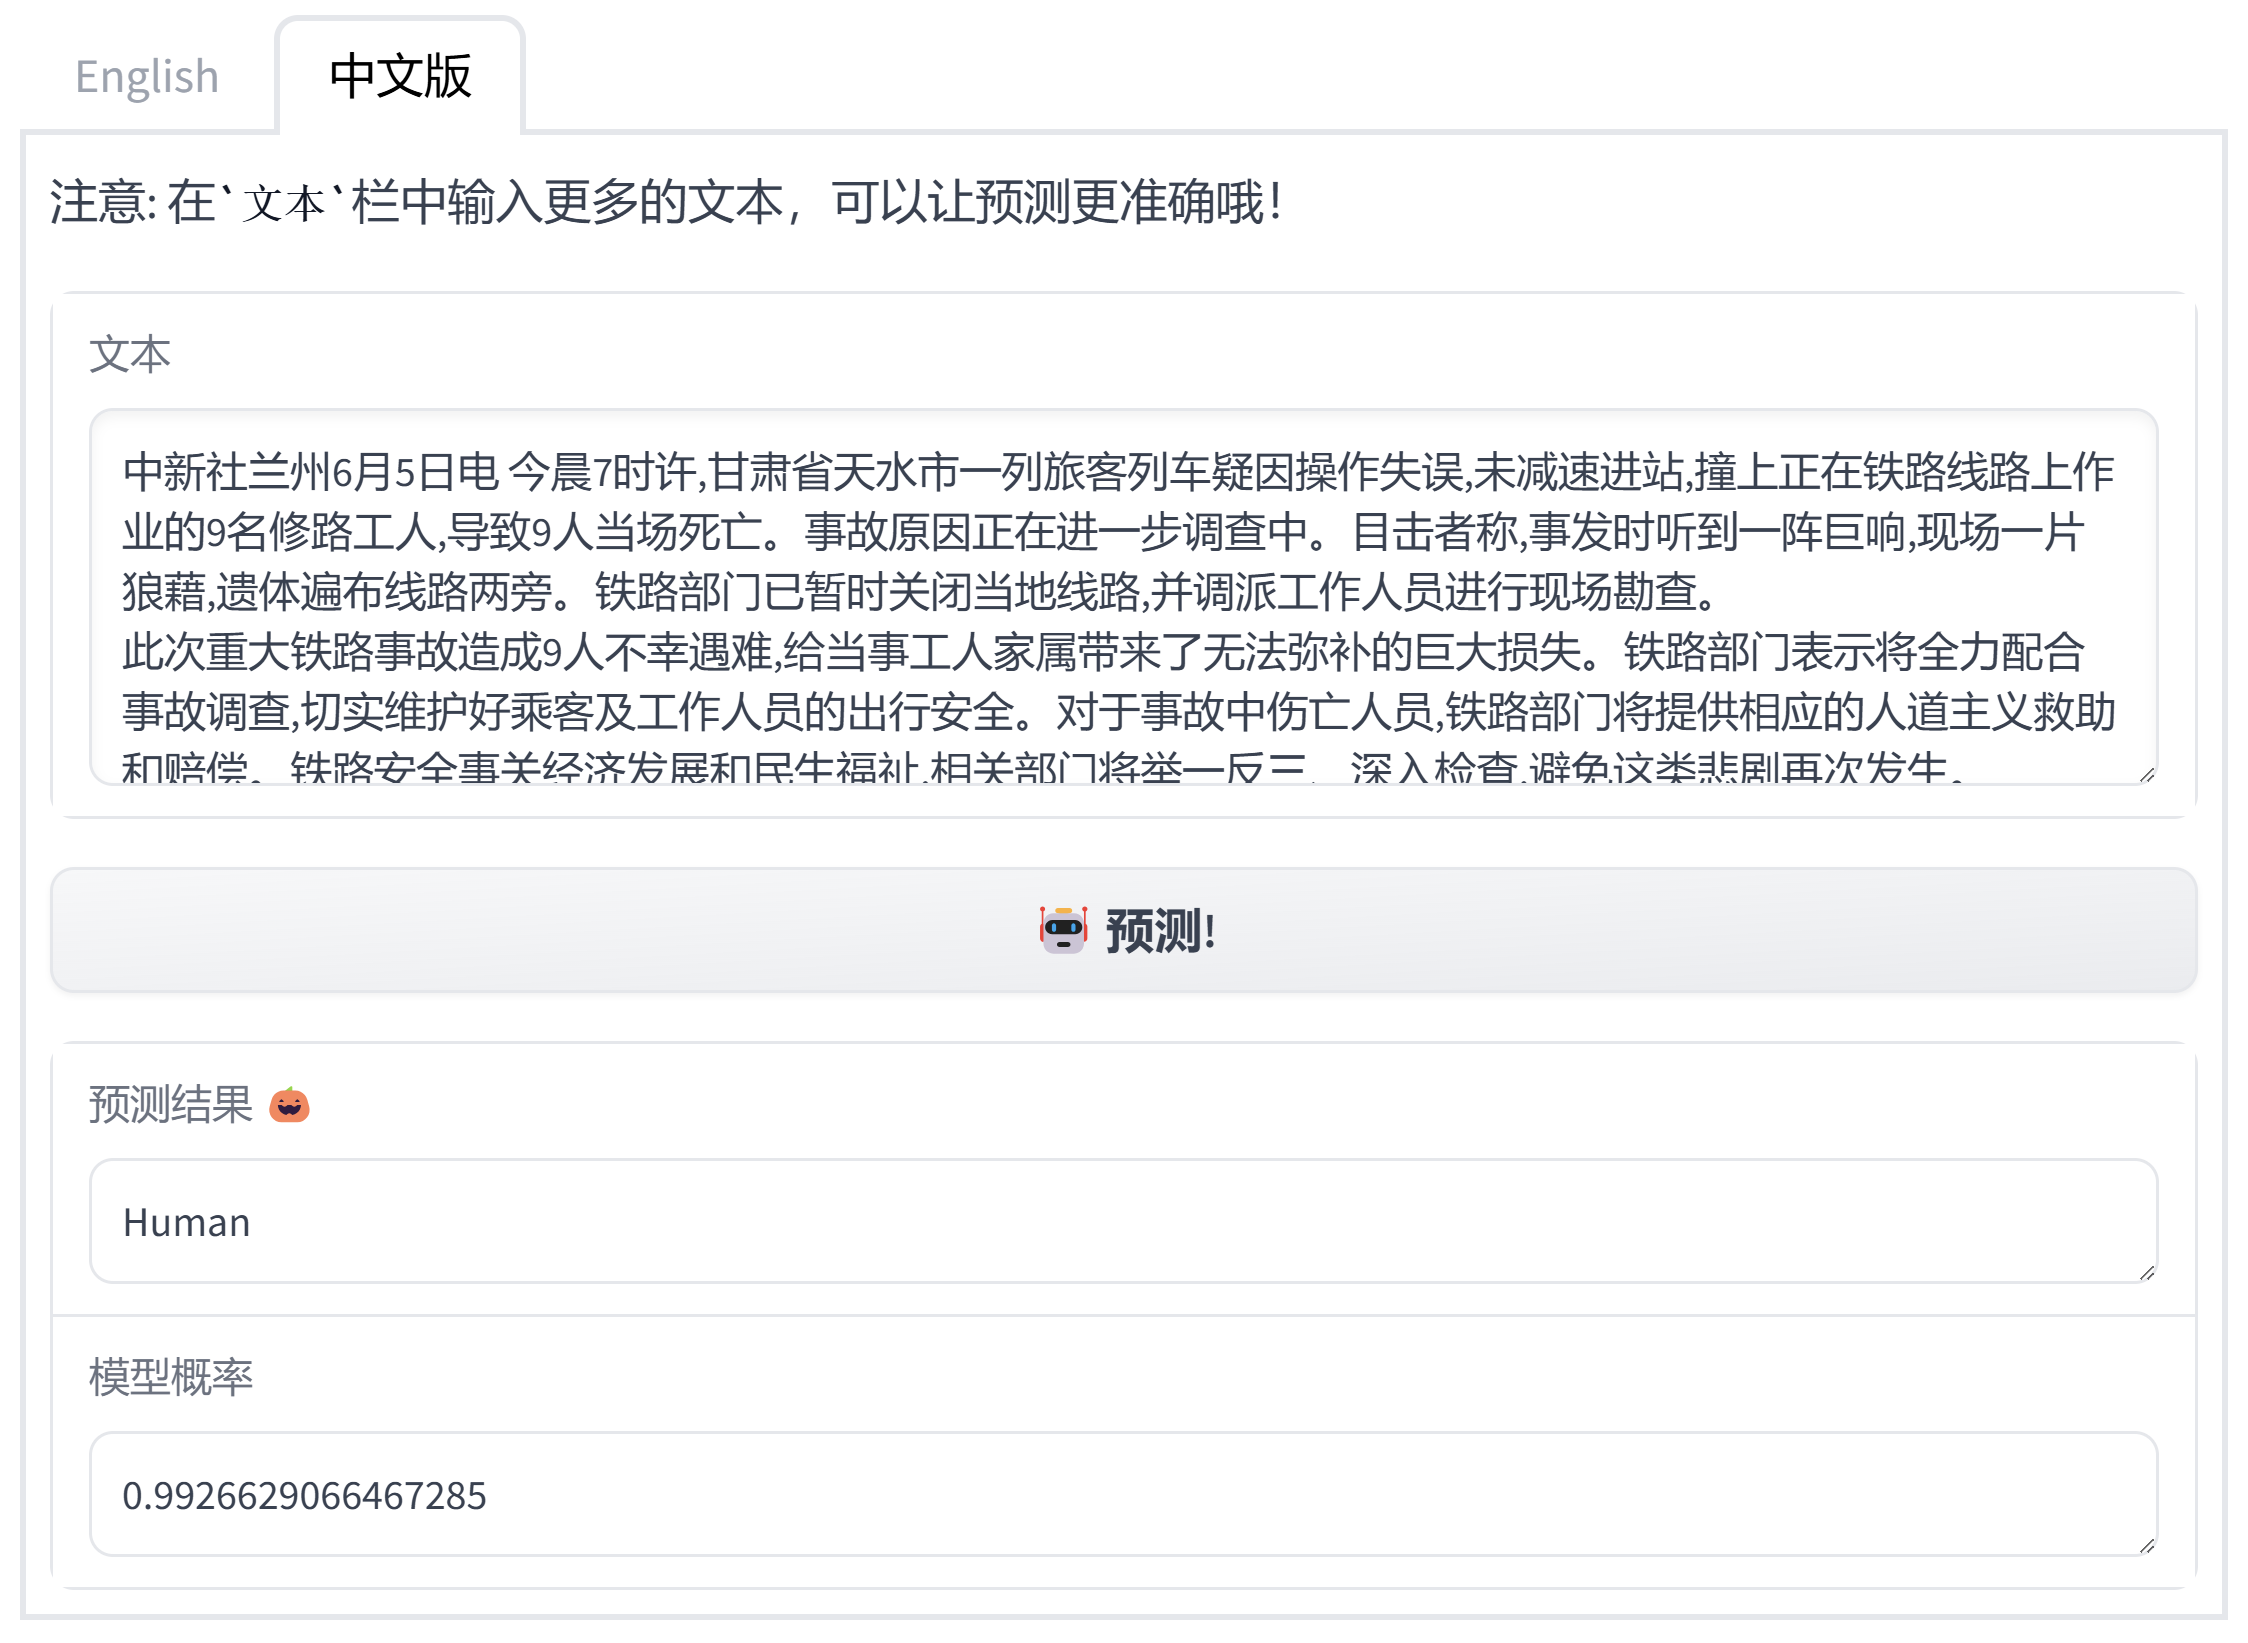
\includegraphics[width=0.8\textwidth]{Claude3_HC3.png}
	\caption{HC3数据集作者开发的检测工具对Claude3 Sonnet生成文本的检测结果显示为人类生成}
	\label{fig:Claude3_HC3}
\end{figure}
同时,中文领域的机器生成文本检测缺乏一个行业公认的性能评估标准测试,二元文本分类模型无法通过这样的一个公认的基准测试,来评估自身的分类性能。
\section{系统概述}
针对现有相关工作的主要问题,我们开发了“星鉴”——支持多域多模型的机器生成文本检测系统,旨在提高中文机器生成文本的检测效果、准确性和泛化性。

“星鉴”中的“星”象征着大量的文本数据,如同浩瀚的星空,寓意广阔无垠,同时也象征着系统的广泛适用性和多域多模型检测能力;“鉴”代表鉴别、检测,体现了系统的核心功能---机器生成文本检测。“星鉴”意味着通过先进的技术手段,如同使用星象仪观察星空一般,精确地检测和分辨机器生成的文本。

\subsection{设计与实现概述}

我们的系统主要分为前端和后端两个部分,前端负责接收用户提交的文本或文件,后端对接收到的文本或文件进行预处理,然后经过分类模型的评估,将检测的结果返回给前端,供用户查看。

前端主要工作为UI设计,我们提供了简洁美观度交互界面,给用户良好的体验。后端部分我们实现了一个结合监督学习与零样本检测方法的二元文本分类模型,可以有效的鉴别中文文本是由人类撰写还是机器生成的。

针对现有中文数据集的不足,我们构建了多域多模型的中文数据集---“瀚海”数据集并在瀚海数据集上训练了我们的监督学习分类模型。同时针对现有中文领域,机器生成文本检测方法性能评估领域的空白,我们设计了“瀚海”Benchmark,可以作为行业的一项性能测试。

\subsection{创新点概述}

我们的工作创新点包括技术和工程两个部分:\textcircled{1}技术上我们提出了结合监督学习与零样本检测方法的二元文本分类方法。\textcircled{2}工程上我们构建了多域多模型的中文数据集“瀚海”,以及可以作为中文领域机器生成文本检测性能评估的“瀚海”Benchmark。

\textbf{针对模型域外效果不佳的问题,我们提出了结合监督学习与零样本检测方法的二元文本分类方法,显著提高了泛化性和抗攻击能力}。具体而言,当前基于预训练模型的监督学习检测方法在域内检测性能极佳,但是泛化性不佳遇到域外的数据检测性能会大幅度下降,零样本检测方法泛化性好,但是检测性能不假为了,因此我们提出了结合监督学习与零样本检测方法的二元文本分类方法,能同时结合两种方法的优势,同时保持高检测性能和高泛化性。

\textbf{针对中文数据集匮乏的问题,我们构建了包含十个大类超过50个话题的中文数据集,同时覆盖了当前各类主流大语言模型,提高了监督学习检测模型的准确性和泛化性。}我们将这个数据集命名为“瀚海”数据集,意为我们的数据集和海一样浩瀚深邃。

数据集的质量直接影响训练出来模型的性能。我们发现当前数据集存在以下两个主要问题:\textcircled{1}中文数据集缺乏,现有的中文数据集主要来自HC3、M4等,数据量较少且领域覆盖不够全面,无法满足多样化需求。\textcircled{2}当前缺少多模型生成文本的数据集,例如HC3数据集的机器生成文本均来自ChatGPT,因此模型提取的特征与ChatGPT高度相关,缺乏泛化能力。这导致当前主流的文本检测工具如GPTzero、Fast-DetectGPT等在检测英文文本时效果较好,但在面对中文文本时准确度明显下降,且对于非ChatGPT的语言模型检测效果较差。

针对上述问题,我们构建了一个包含十个大类超过50个话题的中文数据集,覆盖了学术与专业文献、生活与日常、新闻与媒体、艺术与文化、商业与经济、科技与创新等领域,并从包括ChatGPT、Claude3、讯飞星火等多个大模型中获得数据,使得数据来源多样化,最终实现文本检测方法的跨领域和跨模型的高效检测,大幅提高检测的准确性与泛化性。

\textbf{针对现有中文领域,机器生成文本检测方法性能评估领域的空白,我们设计了“瀚海”Benchmark}。“瀚海”中文Benchmark涵盖学术,新闻,评论,诗歌,医疗,对话,动态等七个领域,包含了超过5000条中文人类撰写文本和机器生成文本的对比条目,调用了国内外一系列大模型包括ChatGPT,Claude3,讯飞星火,文心一言,通义千问,Kimi的API,采取了一系列Prompt工程进行构建,可以为后续中文领域机器生成文本检测方法提供一项性能基准测试。

\chapter{作品设计}
\section{软件开发流程概述}
在整个软件开发过程中,我们选择以 V 模型作为指导开发的流程,以明确每个阶段的工作和相应的验证步骤。V 模型是软件开发生命周期模型的一种,其结构类似于字母“V”,体现了开发与测试的并行进行。相比于其他模型,V 模型的显著优势在于它将验证与验证紧密结合,每个开发阶段都有对应的测试阶段。这种方式不仅确保了问题的早期发现和解决,还提高了软件开发的质量和可靠性,从而大幅降低了后期维护和修复的成本。V模型结构如图\ref{fig:V-Model}所示。
\begin{figure}[H]
	\centering
	\includegraphics[width=0.8\textwidth]{figures/V-Model.png}
	\caption{V模型示意图}
	\label{fig:V-Model}
\end{figure}
在 V 模型的左侧部分,开发阶段包括需求分析、概要设计、详细设计和编码,这些步骤逐步细化系统的功能和结构;而在右侧部分,每个开发阶段对应的测试阶段依次是单元测试、集成测试、系统测试和验收测试,确保每个阶段的输出都经过严格验证。

需求分析过程中,基于1.1.2、1.2和1.3小节的调研结果,我们发现中国互联网规模庞大,网民数量巨大,对于机器生成文本检测工具的需求广泛,中文环境下的机器生成文本检测系统具有广阔的应用前景。在此背景之下,当前主流检测工具如GPT-zero、FastDetectGPT等对中文文本的检测效果不够理想,而国内提供的检测工具检测存在工具使用流程繁琐、准确率较低、应用范围局限、价格昂贵等问题,如当前已经被众多高校采用的维普AIGC检测工具主要提供针对论文的检测,应用场景局限,且检测费用高达20元/篇,提高了检测的使用门槛。为此我们计划开发“星鉴”文本检测系统来弥补中文检测领域的空缺,我们的目标是实现行业领先的中文检测效果。

概要设计过程中,我们将任务分成了四个板块,分别为数据集构建、模型训练、后端开发、前端开发。\textbf{针对数据集构建},我们计划是构建一个多域多模型的中文数据集,并将其取名为“瀚海”数据集。我们将收集10个不同领域的人类回答和机器回答,并进行标注。同时,机器回答文本将包含多个模型,以提高模型检测的准确率和泛化能力。\textbf{针对分类模型构建},考虑到python在机器学习领域有着丰富的库生态、简洁易用的语法、高效的开发效率、良好的跨平台性以及成熟的科学计算功能,我们最终选择以python语言实现模型的训练。实现方法上,基于1.3小节的分析,我们将基于监督学习和零样本检测相结合的方法实现一个二元文本分类模型。\textbf{针对后端开发},我们同样选择以python作为开发语言,理由是python提供了强大的文件处理能力以及丰富的科学计算功能。我们计划将前端输入的文本或上传的文件传入后端后,由后端调用模型接口完成对文本或文件的检测,并在后端实现对文本或文件的标注处理。\textbf{针对前端开发},我们计划做出一个简洁且美观的界面,各个功能板块划分清晰,交互效果灵动。此外界面主题色选择应该与“星鉴”和“瀚海”的意境相同,我们将主题色定为蓝色。%

详细设计的内容我们将会在2.3小节探讨,具体实现过程我们会在第3节进行详细说明。

软件测试过程中,分工和各个流程工作概述如下:\textbf{单元测试中},各模块负责人应对其负责的模块进行全面、详细的测试,验证每个功能点的执行结果是否与预期一致。这包括在正常和异常情况下的表现。此外,还需确保模块之间的接口正确无误,保证数据传递和交互的准确性。同时,需测量模块的响应时间、准确率和资源占用等性能指标,并将其与预期目标进行对比,确保其满足性能要求。\textbf{集成测试中},由指定的同学负责进行集成测试,检测各个板块在继承之后的功能,确保前端和后端的各个模块能够无缝集成,并且整体系统能够稳定运行。\textbf{系统测试中},由组长负责进行系统测试,全面测试整个系统的功能和性能,确保所有模块和子系统的协调运行,验证系统在各种使用场景下的稳定性和可靠性。\textbf{验收测试中},由指导老师负责进行验收测试,对系统进行最终评估,确保其达到了所有预期目标。最终的测试结果将会在第3章和第4章中详细介绍。

\section{系统设计}
\subsection{总体系统架构}
系统架构如图\ref{总体系统架构}所示。本系统包括客户端和服务端,用户通过客户端上传需要检测的文本或者文件,发送给服务端,服务端对客户端传送过来的文本和文件进行处理,并将检测结果发送回客户端。
\begin{figure}[H]
	\centering
	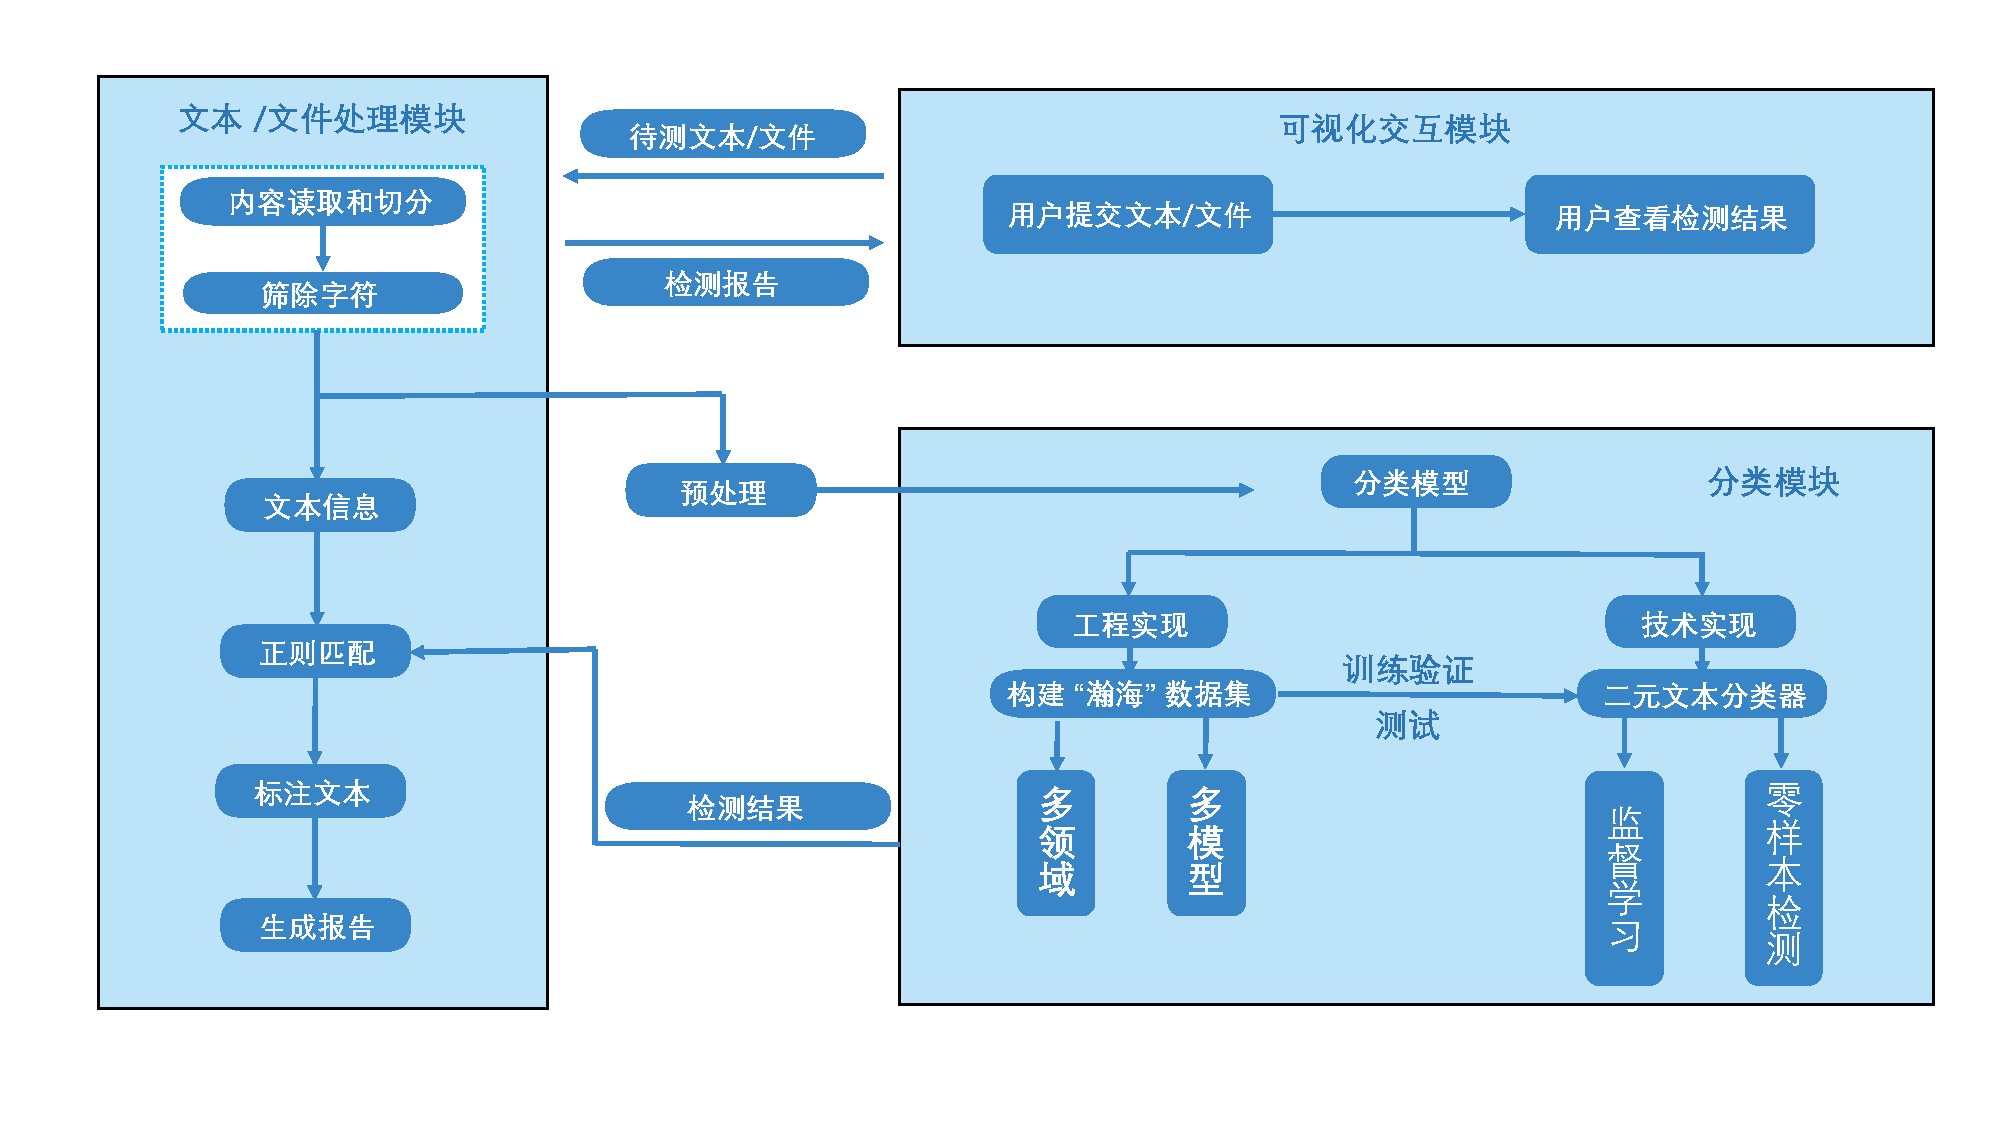
\includegraphics[width=1\textwidth]{figures/系统架构图.pdf}
	\caption{总体系统架构}
	\label{总体系统架构}
\end{figure}

\subsection{系统功能}
本系统支持多个领域多个模型生成文本的文本检测,下表描述了本系统的基本功能
\begin{table}[H]
	\centering
	\begin{tabular}{cc}
		\toprule
		\textbf{功能列表} & \textbf{功能描述}                        \\ \midrule
		文本检测功能        & 用户在客户端输入一段文本,检测完成后会返回这段文本由机器生成的概率    \\ \midrule
		文件检测功能        & 用户可以上传PDF,DOCX和TXT格式的文件,检测完成后会返回检测报告 \\ \midrule
		图像提取功能        & 用户可以上传图像,系统会提取图像中的文字,允许用户编辑后进行检测     \\      \midrule
		深度文本分析        & 文本检测完会告知用户各段落由机器生成的概率,并标识各个成分的占比     \\ \midrule
		文件标注功能        & 根据段落评估概率,标注高亮,并标注各段落的生成概率            \\
		\midrule
	\end{tabular}
	\caption{系统功能}
	\label{系统功能}
\end{table}
\section{模块设计}
系统主要分为客户端和服务端两个大板块,客户端主要负责用户交互,服务端主要负责文本检测。我们将分板块对每一个部分的每一个模块进行介绍。
\subsection{服务端设计}
在服务端设计过程中,我们深入分析了用户需求。针对最基本的文本检测功能,我们发现用户通常习惯直接输入文本,并更关注直接的检测结果,因此我们没有对输入文本长度做任何上限限制。同时如果文本过长输入不便,则可以上传TXT文件进行检测。考虑到当前绝大多数文献和办公文件都是以PDF和DOCX形式,我们还增加了对PDF以及DOCX文件的检测支持,系统将以不同颜色标注不同段落中机器生成的概率,使用户能够清晰地看出文档中机器生成的部分,从而更方便地对长文档进行检测。考虑到有的文本是以扫描件的形式存在,我们还加入了OCR识别功能,允许用户上传图片形式的文档,自动提取图片中文字内容进行检测。最后,在检测过程中需要提供实时反馈,以确保用户知道检测正在进行。

关于文本检测功能的详细设计思路如下:
\begin{enumerate}
	\item \textbf{输入文本检测。} 直接判断文本为机器生成的概率,概率越高表示文本中存在机器生成的痕迹越明显。在短文本中可以直接显示机器生成的概率
	\item \textbf{TXT文件检测。} 设计切分固定长度文本片段并检测每个切片为机器生成的概率。
	\item \textbf{PDF和DOCX文件检测。} 上传 PDF和DOCX文件,返回各个切片的检测结果,并以不同颜色标注,如红色代表机器生成,黄色代表疑似机器生成,无色代表人类生成,同时返回一个整体的检测报告
	\item \textbf{图片内容提取检测。}  上传图片形式的文件,先使用OCR识别模块,自动提取图片中的文本,返回文本检测模块,允许用户自行编辑修改后进行检测。
	\item \textbf{文本深度分析。}对文本进行深度分析,判断不同段落由机器生成的概率。
\end{enumerate}

而文本检测功能的核心是我们的二元检测分类模型,这也是“星鉴”系统的核心。我们的二元检测分类模型设计思路如下:
\begin{enumerate}
	\item \textbf{监督学习分类模块}使用 XLM-RoBERTa-Base 多语言版本自编码器预训练语言模型作为特征提取器,对输入文本进行深度语言特征的提取。为了解决传统监督学习方法泛化性差以及难以拓展到多语言的问题,我们同时使用多领域、多模型的多语言(“星鉴”目前聚焦于中文与英文)标记数据进行训练。
	\item \textbf{零样本检测分类模块}使用国产的 Qwen2-0.5B 生成式预训练语言模型进行采样与自信息丰富度计算。由于人类文本在进行采样的时候不确定性会更大,因此计算得到样本与原文自信息差异的波动会远大于机器文本,因此我们参考了统计学中变异系数的概念,使用样本与原文自信息差异的标准差除以样本与原文自信息差异的均值,得到了自信息丰富度(SIR),根据我们的实验验证,人类文本的自信息丰富度会大于机器文本。
	\item \textbf{监督学习与零样本检测的结合}是根据监督学习的特性而进行设计的,我们选择 $[0, 0.2) \cup (0.8, 1] $作为置信区间,这样在域内外的数据上都能有超过$0.99$的置信度。对于置信区间内的高置信度数据,我们直接使用监督学习进行检测即可,对于置信区间外的低置信度数据,我们需要调用零样本检测分类器。因此我们能同时保留监督学习的高速与域内高准确性,以及零样本检测的高泛化性能力。

\end{enumerate}


\subsection{客户端设计}
在客户端设计过程中,我们深入分析了用户需求,明确用户在网页交互中的核心需求为界面美观且简洁、信息获取便捷、高效的功能体验以及全面的支持与指导。基于这些需求,我们计划先完成三个模块:作品简介、文本检测、常见问题。

\begin{enumerate}
	\item \textbf{作品简介模块}将作为用户访问的首页。我们将对作品进行简洁明了的介绍,突出关键信息,帮助用户快速了解作品的核心内容和特点。这一模块的设计注重信息的直观展示,使用户能够一目了然地获取所需信息。

	\item \textbf{文本/文件检测模块}致力于提供一种方便且高效的文本检测服务。用户可通过此模块中的输入框提交文本以进行检测。为了增强用户体验,我们拟在输入框旁边添加一个环形图来可视化检测结果。在文本框下方我们将会提供深度检测分析栏,用户输入的文本将在深度检测过程中依照概率被划分为不同颜色。同时,我们还将提供上传文件的功能,允许用户上传文档进行检测。该模块的设计目标是提升用户体验,确保文本检测过程简单易用。

	\item \textbf{常见问题模块}将涵盖用户在使用过程中可能遇到的问题及其解答。此外,我们还将把README文档放在此模块中,详细介绍我们的软件产品和模型部署的相关信息。这一模块的设计旨在为用户提供全面的支持和指导,帮助用户顺利使用我们的产品。

\end{enumerate}

通过这三个模块的设计,我们力求满足用户的需求,提供一个功能全面、操作简便的网页客户端,最终为用户提供一个友好且高效的使用体验。最终客户端的设计原型图如图\ref{fig:Web_model}所示。
\begin{figure}[H]
	\centering
	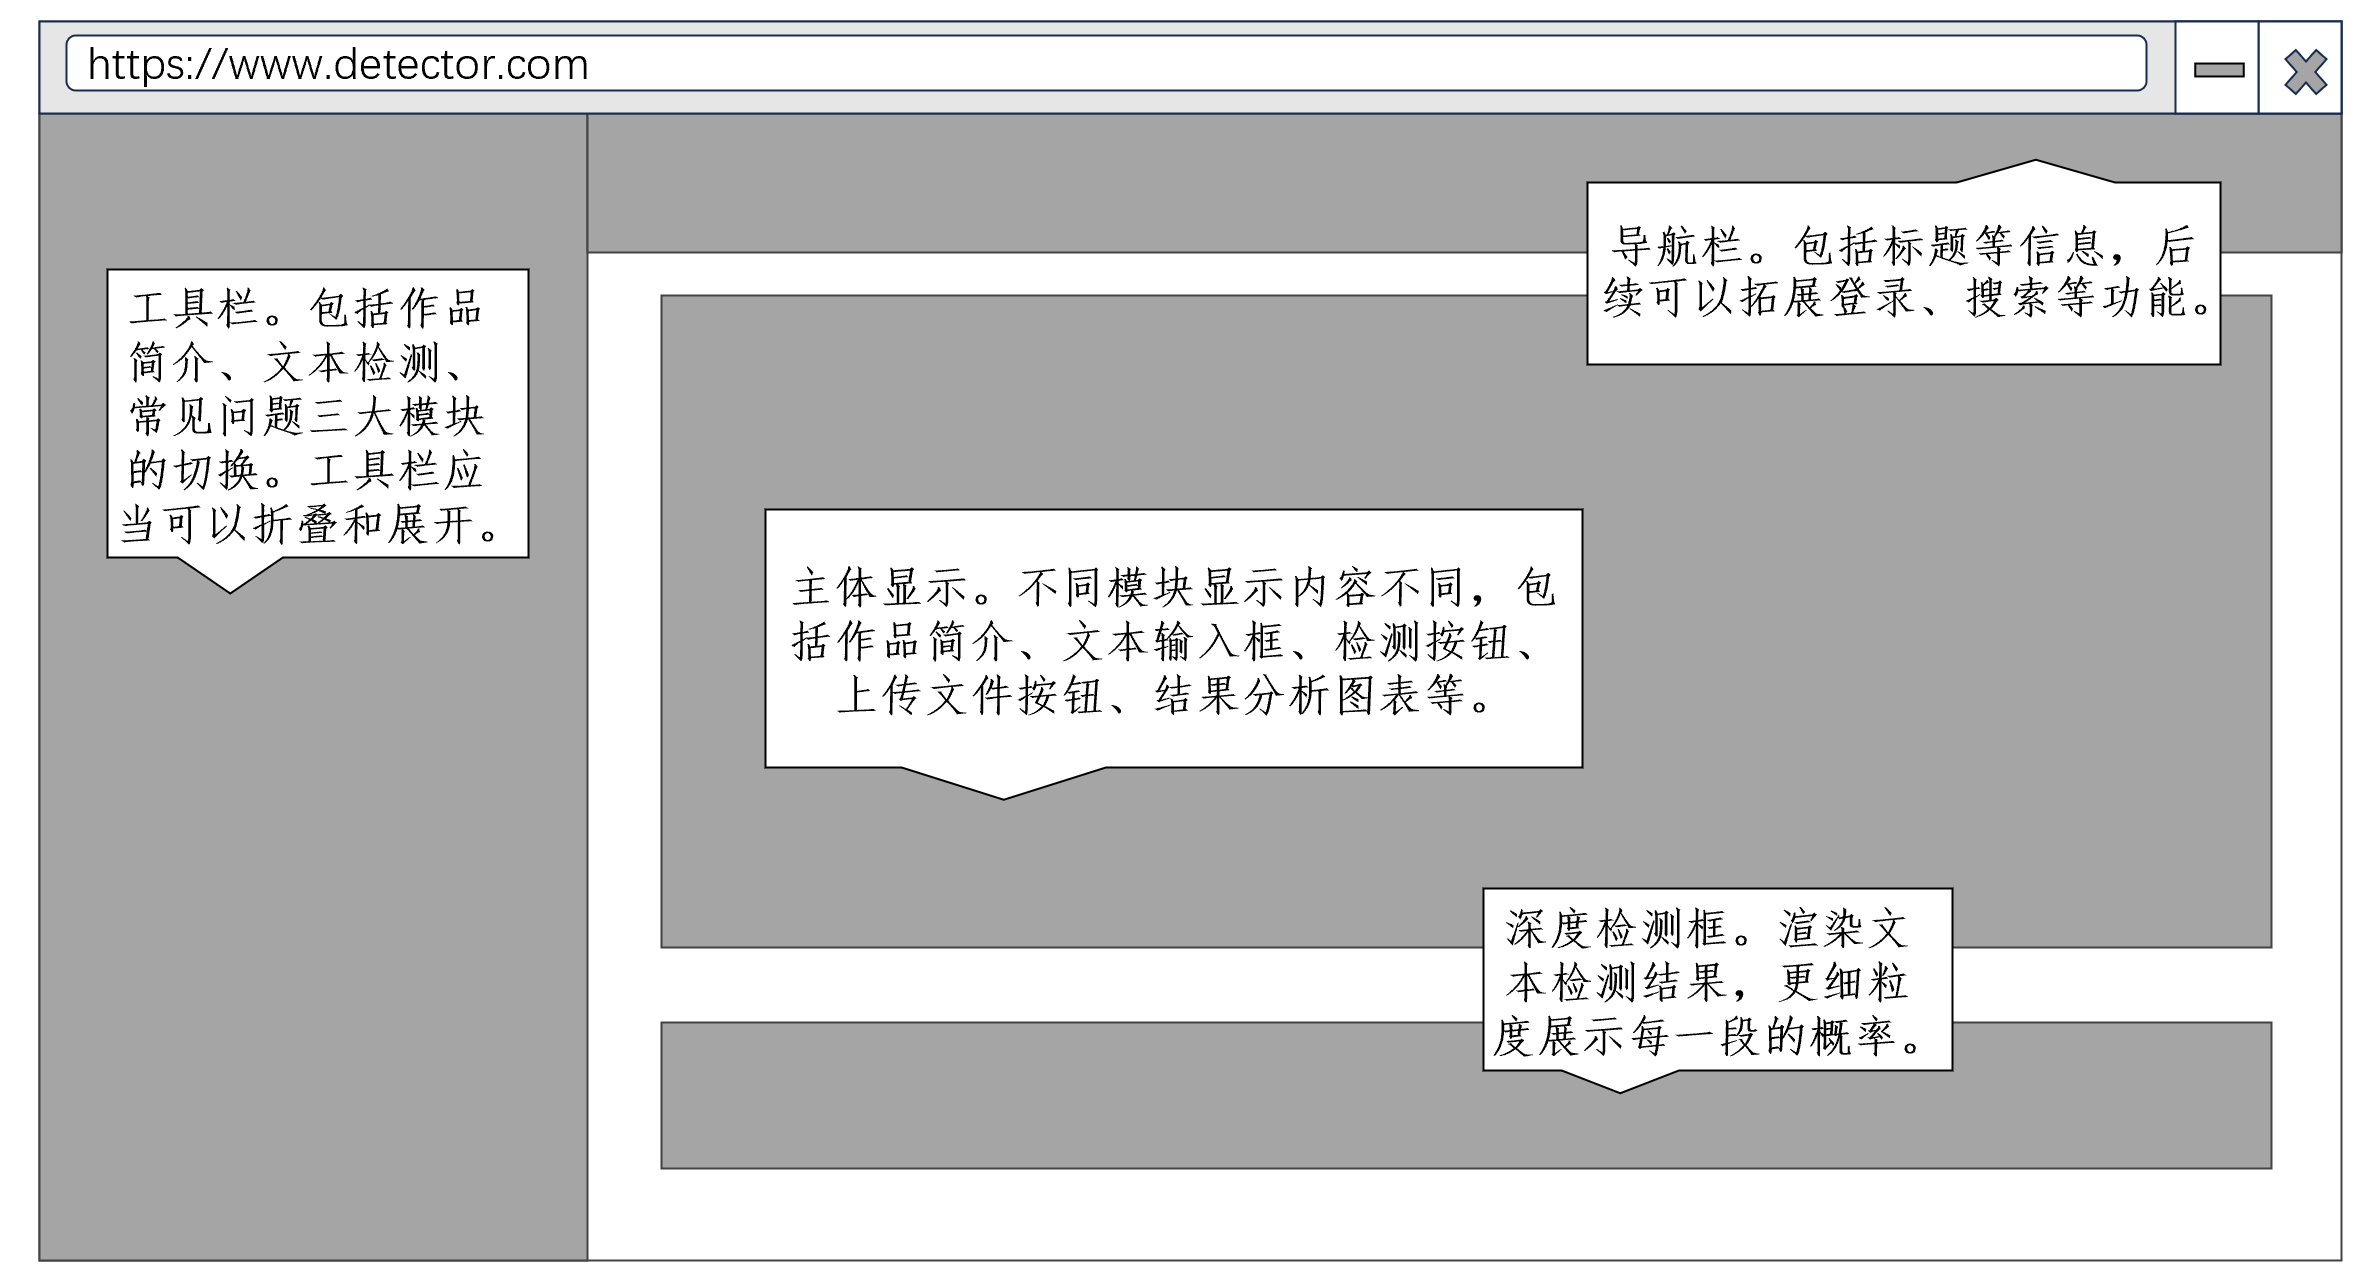
\includegraphics[width=0.85\textwidth]{figures/Web_model.png}
	\caption{客户端设计原型图}
	\label{fig:Web_model}
\end{figure}
%瀚海数据集不急,这个要好好重写
\chapter{作品实现}

\section{结合监督学习与零样本检测方法的二元文本分类模型}
“星鉴”系统采用了一种结合结合监督学习与零样本检测的创新性方法,构建了一个高效的二元文本分类模型。该模型的主要任务是对输入文本进行分类,以判断其是由人类生成还是由机器生成。
具体来说,我们定义文本分类的目标函数$D(\vec{x})$,$\vec{x}$为一段文本,那么$D(\vec{x})$可以表示为:
\begin{equation}
	D(\vec{x})=\begin{cases}
		1, & \text{如果文本$\vec{x}$由机器生成} \\
		0, & \text{如果文本$\vec{x}$由人类生成}
	\end{cases}
\end{equation}
整个文本分类模型主要包括两个核心模块:\textbf{监督学习分类器模块}与\textbf{零样本检测分类器模块}。

\textbf{监督学习分类器模块}使用XLM-RoBERTa-Base多语言版本自编码器预训练语言模型作为特征提取器,对输入文本进行深度语言特征的提取。RoBERTa能够捕捉到丰富的上下文信息和细粒度的语言特征。给定输入文本$\vec{x}$,RoBERTa模型会输出一个高维特征向量表示:

\begin{equation}
	\mathbf{h}_{\vec{x}} = \text{RoBERTa}(\vec{x})
\end{equation}

然后将提取的特征向量$\mathbf{h}_{\vec{x}}$传送给一个三层的多层感知器(MLP),让MLP进行分类决策。MLP将高维特征向量映射到概率空间$[0,1]$,输出文本分类的预测概率$P(\vec{x})$,$P(\vec{x})$越接近1代表文本由机器生成的概率越大。

为了解决传统监督学习方法泛化性差以及难以拓展到多语言的问题,我们同时使用多领域、多模型的多语言(“星鉴”目前聚焦于中文与英文)标记数据进行训练,实验表明这种做法可以提高准确率以及泛化性,并且拓展到新语言的时候不需要再使用其他的预训练模型,只需要增加少量的对应语言标记数据即可。

\textbf{零样本检测分类器模块}的实现基于一个已经被验证的前提:人类在撰写文本中根据语境选择更加多样化的Token,而机器则会基于语言模型的概率来进行Token选择,因此机器会倾向于选择高概率Token。该前提的根源在于这样一个事实,即预训练语言模型反映着人类的集体写作行为,而不是人类个体的写作行为,这就导致了人类与机器在给定上文情况下的Token选择存在差异。根据这个前提,我们提出假设:人类文本的自信息丰富度更有可能为正值,而机器文本的自信息丰富度更接近于零。具体而言,人类文本的\textbf{自信息丰富度}集中在1左右,而机器文本的\textbf{自信息丰富度}集中在0左右。自信息丰富度的定义详见3.2.2小节。

自信息丰富度反映了采样文本与原文本的自信息分布差异,由于平均意义上人类文本的自信息分布比机器文本更离散,因此采样后的人类文本与原文本的自信息均值与标准差的差异会大于机器文本,因此平均意义上人类文本的自信息丰富度会大于机器生成文本,这也是开发“星鉴”零样本检测分类器模块的核心原理。

“星鉴”巧妙的将监督学习方法与零样本检测结合。由于监督学习的特性,当置信度大于0.99时,域内外数据的检测概率都会落在$[0,0.2)\cup(0.8,1]$区间内。因此可以根据这个特性来区分高置信度数据与低置信度数据。高置信度数据直接由监督学习分类器进行二元分类即可,低置信度数据则交给零样本检测分类器。“星鉴”系统通过监督学习与零样本检测的有效结合,实现了高效且精准的文本分类,能够在实际应用中准确快速的区分人类生成和机器生成的文本。

%此处需要一张监督学习与零样本检测结合的架构图

\subsection{监督学习分类器模块}
监督学习分类器一个很经典的做法就是使用预训练语言模型RoBERTa作为特征提取器,然后将嵌入层的高维向量传送至线性层进行分类决策。但是这种传统的做法会带来两个问题:一是域外数据检测效果不佳,泛化性较差;二是每增加一种语言就需要增加一个新语言版本的RoBERTa以及对应的分类模型,这会导致最终的系统非常庞大,训练成本大幅增加。

为了缓解泛化性不佳,解决难以拓展到其他语言的问题,“星鉴”使用XLM-RoBERTa-Base多语言版本自编码器预训练语言模型,并且直接使用多语言(“星鉴”主要聚焦与英文与中文)的标记数据进行训练,这样不仅提高了准确性以及泛化性,并且拓展到其他语言时只需要增加少量的对应语言标记数据,不需要重新准备一个新的语言版本的自编码器预训练语言模型。这种创新的做法使得“星鉴”在保持精准高效的同时,保证了轻量化。
\begin{table}[H]
	\centering
	\begin{tabular}{lcccccc}
		\toprule
		\textbf{模型}      & \textbf{Accuracy} & \textbf{Precision} & \textbf{Recall}  & \textbf{F1}      & \textbf{ROC-AUC} \\
		\midrule
		RoBERTa-base     & 0.8303            & 0.8640             & 0.7831           & 0.8216           & 0.8302           \\
		星鉴监督学习分类器模块      & 0.8923            & 0.9071             & 0.8738           & 0.8901           & 0.8921           \\
		\midrule
		\textbf{提升 (\%)} & \textbf{+6.20\%}  & \textbf{+4.31\%}   & \textbf{+9.07\%} & \textbf{+6.85\%} & \textbf{+6.19\%} \\
		\bottomrule
	\end{tabular}
	\caption{星鉴监督学习分类器模块与RoBERTa-base在监督学习域外的性能比较}
	\label{tab:性能提升}
\end{table}

在编码器中,每个词都会被映射到一个连续的向量空间,用于捕捉该词的语义信息。设输入序列的长度为 $n$,每个词的向量表示为 $x_i$,其中 $i \in \{1, 2, ..., n\}$。经过 $l$ 个编码层的转换和计算,每个词的向量都会被更新,融合了更多的上下文语义信息,更新后的向量表示为 $h_i$,其中 $i \in \{1, 2, ..., n\}$。

在分类模块中,我们采用了多层感知器(MLP)作为分类器。“星鉴”中MLP 由三个全连接层组成,每一层都对输入向量进行了线性变换和非线性激活,以提取更高层次的特征表示。设 MLP 有 $L$ 个全连接层,第 $l$ 层的输出向量为 $a_l$,其中 $l \in \{1, 2, ..., L\}$。那么 MLP 的最终输出向量 $y$ 可以表示为:

\begin{equation}
	y = a_L
\end{equation}

每一层的全连接层都会对上一层的输出向量 $a_{l-1}$ 进行线性变换,并加上偏置项 $b_l$。设第 $l$ 层的权重矩阵为 $W_l$,则第 $l$ 层的输出向量 $a_l$ 可以计算为:

\begin{equation}
	a_l = W_l a_{l-1} + b_l
\end{equation}

MLP的输入层与隐藏层采用了ReLU作为激活函数,输出层使用Sigmoid 激活函数,将输出映射到在 [0, 1] 的概率区间之内,越接近1说明文本由机器生成的概率越大。

在训练阶段,我们采用交叉熵损失函数来优化模型参数,衡量模型预测的概率分布与真实标签分布之间的差异。设样本的真实标签为 $y_i$,其中 $i \in \{1, 2, ..., n\}$,模型预测的第 $i$ 类概率为 $p_i$,则交叉熵损失函数可以表示为:

\begin{equation}
	L = -\sum_{i=1}^n y_i \log(p_i) + (1 - y_i) \log(1 - p_i)
\end{equation}

通过最小化上述损失函数,我们可以不断调整模型参数,使得模型预测的概率分布尽可能逼近真实标签分布,从而提高分类性能。


\subsection{零样本检测分类器模块}

“星鉴”的监督学习分类器模块无法从根本上解决泛化性不佳的问题,只能进行缓解。因此,引入零样本检测分类器模块是必要的。以往的零样本检测方法解决了监督学习的泛化性问题,但是计算成本过高,速度太慢。以去年的SOTA方法Fast-DetectGPT为例,它需要使用预训练语言模型GPT Neo-2.7B,如此庞大的模型,至少需要一张NVIDIA GeForce RTX 3090 24GB才可能部署,并且推理速度也相对较慢。并且经过我们验证,Fast-DetectGPT所提出的“条件曲率”在换用更小的预训练模型会失效,通用性不佳。为了解决这些问题,我们提出了全新的零样本检测方法,在保证高准确率高泛化性的前提下,极大程度的减少了计算开销,并且比Fast-DetectGPT快10倍以上。

“星鉴”的零样本检测分类器模块使用国产的Qwen2-0.5B生成式预训练语言模型。对于给定的文本$\vec{x}$和生成式预训练语言模型$P_{\theta}$,首先使用预训练模型对每个Token(记为$x_i$,$i$表示从前往后计数的第$i$个Token)进行采样,每个Token处得到一个包含10000个采样Token的样本集合,记为$\hat{X_i}$($i$表示从前往后计数的第$i$个Token,注意这里$\hat{X_i}$是一个包含10000个采样Token的集合),同时在给定上文的前提下,对于每一个位置的Token,通过预训练语言模型得到所有样本的生成概率$P(\hat{X_i})$,计算所有样本自信息量$I(\hat{X_i})=-\log(P(\hat{X_i}))$的均值与标准差,分别记为$\mu(I(\hat{X_i}))$和$\sigma(I(\hat{X_i}))$。然后对于整个文本,我们计算所有Token样本的$\mu(I(\hat{X_i}))$和$\sigma(I(\hat{X_i}))$对应的均值和标准差,分别记为:
\begin{equation}
	S_{\mu\mu} = \frac{1}{N} \sum_{i=1}^N \mu(I(\hat{X_i}))
\end{equation}

\begin{equation}
	S_{\mu\sigma} = \sqrt{\frac{1}{N} \sum_{i=1}^N \left( \mu(I(\hat{X}_i)) - S_{\mu\mu} \right)^2}
\end{equation}

\begin{equation}
	S_{\sigma\mu} = \frac{1}{N} \sum_{i=1}^N \sigma\left(I\left(\hat{X_i}\right)\right)
\end{equation}

\begin{equation}
	S_{\sigma\sigma} = \sqrt{\frac{1}{N} \sum_{i=1}^N \left( \sigma\left(I\left(\hat{X_i}\right)\right) - S_{\sigma\mu} \right)^2}
\end{equation}


同时,我们计算文本$\vec{x}$的自信息量$I(x_i)$的均值与标准差,分别记为:

\begin{equation}
	O_{\mu} = \frac{1}{N} \sum_{i=1}^N \mu(I(x_i))
\end{equation}

\begin{equation}
	O_{\sigma} = \sqrt{\frac{1}{N} \sum_{i=1}^N \left( \mu(I(x_i)) - O_{\mu} \right)^2}
\end{equation}


在此基础上,我们定义自信息丰富度(self-information richness,SIR)为:
\begin{equation}
	\mathbb{SIR}=\frac{S_{\sigma\sigma}\cdot\Delta\mu}{S_{\sigma\mu}\cdot\Delta\sigma}
\end{equation}
其中
\begin{equation}
	\mathbb{SIR}=\frac{S_{\sigma\sigma}\cdot (O_\sigma-S_{\mu\sigma})}{S_{\sigma\mu}\cdot (O_\mu-S_{\mu\mu})}
\end{equation}

\begin{equation}
	\Delta\sigma=O_\sigma-S_{\mu\sigma}\qquad\Delta\mu=O_\mu-S_{\mu\mu}
\end{equation}

由于人类文本在进行采样的时候不确定性会更大,因此计算得到样本与原文自信息差异的波动会远大于机器文本,因此我们参考了统计学中变异系数的概念,使用样本与原文自信息差异的标准差除以样本与原文自信息差异的均值,得到了自信息丰富度(SIR),根据我们的假设,人类文本的自信息丰富度会大于机器文本。为了验证我们的假设,我们在包含了多领域多模型的中英文人类机器文本数据集(共十万条以上文本)上计算所有文本的自信息丰富度,绘制了一张自信息丰富度分布图:

\begin{figure}[H]
	\centering
	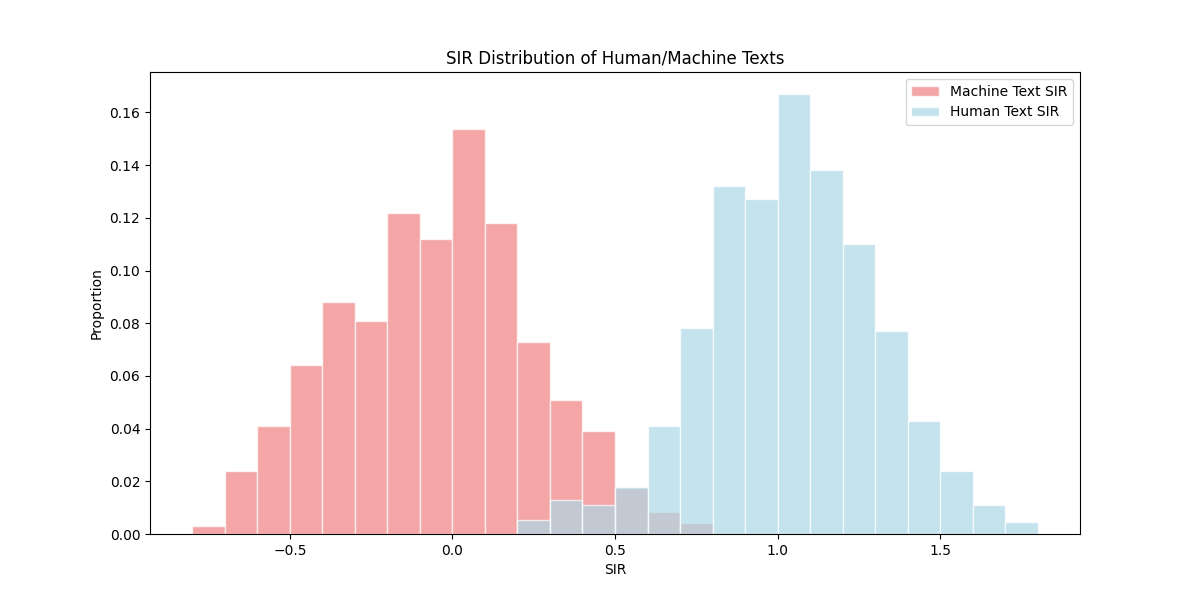
\includegraphics[width=0.95\textwidth]{figures/SIR.png}
	\caption{人类/机器文本自信息丰富度分布差异}
	\label{fig:SIR}
\end{figure}

从图中可以看出,人类和机器文本的自信息丰富度都基本符合正态分布,且人类的自信息丰富度集中在1左右,而机器的自信息丰富度集中在0附近。这也验证了我们的假设,自信息丰富度可以作为分类人类文本与机器文本的依据。

“星鉴”的零样本检测分类器模块进行一次检测时,只需要调用一次预训练语言进行从后向前计算,即可同时完成采样以及自信息丰富度的计算,并且“星鉴”只需要调用Qwen2-0.5B生成式预训练语言模型,模型参数相对较少,只需要4GB显存即可,计算成本低且推理速度极快。


\subsection{监督学习与零样本检测的结合}
虽然“星鉴”的零样本检测模块准确率高,泛化性强,且需要的计算资源较少,但是监督学习分类器的速度明显快于零样本检测,并且监督学习在域内的准确性高于零样本检测方法。因此我们将二者结合,同时保留监督学习的高速与域内高准确性,以及零样本检测的高泛化性。

根据我们的测试,监督学习分类器对于域内数据,在置信度设置为0.999的情形下,置信区间为$[0,0.3589)\cup(0.6824,1]$,在置信度设置为0.99的前提下,置信区间为$[0,0.4357)\cup(0.6621,1]$;对于域外数据,在置信度设置为0.999的情形下,置信区间为$[0, 0.1391) \cup (0.8924, 1]$,在置信度设置为0.99的情形下,置信区间为$[0,0.2415)\cup(0.7926,1]$。

			\begin{table}[H]
					\centering
					\begin{tabular}{>{\centering\arraybackslash}m{4cm} >{\centering\arraybackslash}m{3cm} >{\centering\arraybackslash}m{7cm}}
						\toprule
						\textbf{数据类型}         & \textbf{置信度} & \textbf{置信区间}                  \\
						\midrule
						\multirow{2}{*}{域内数据} & $0.999$      & $[0, 0.3589) \cup (0.6824, 1]$ \\
						                      & $0.99$       & $[0, 0.4357) \cup (0.6621, 1]$ \\
									\midrule
						\multirow{2}{*}{域外数据} & $0.999$      & $[0, 0.1391) \cup (0.8924, 1]$ \\
						                      & $0.99$       & $[0, 0.2415) \cup (0.7926, 1]$ \\
						\bottomrule
					\end{tabular}
					\caption{不同置信度下的域内外数据置信区间}
					\label{不同置信度下的域内外数据置信区间}
				\end{table}

			因此最后我们选择$[0,0.2)\cup(0.8,1]$作为置信区间,这样在域内外的数据上都能有超过0.99的置信度。

对于置信区间之内的高置信度数据,我们直接使用监督学习进行检测即可,对于置信区间以外的低置信度数据,我们才需要调用零样本检测分类器。因此我们能同时保留监督学习的高速与域内高准确性,以及零样本检测的高泛化性能力。

我们通过消融实验来验证“星鉴”每一个模块的必要性。我们分别绘制单监督学习分类器模块,单零样本检测分类器模块,以及二者结合情况下的ROC曲线图,使用的数据集包含监督学习域内数据50\%,域外数据50\%,共5000条人类文本,5000条机器文本。

\begin{figure}[H]
	\centering
	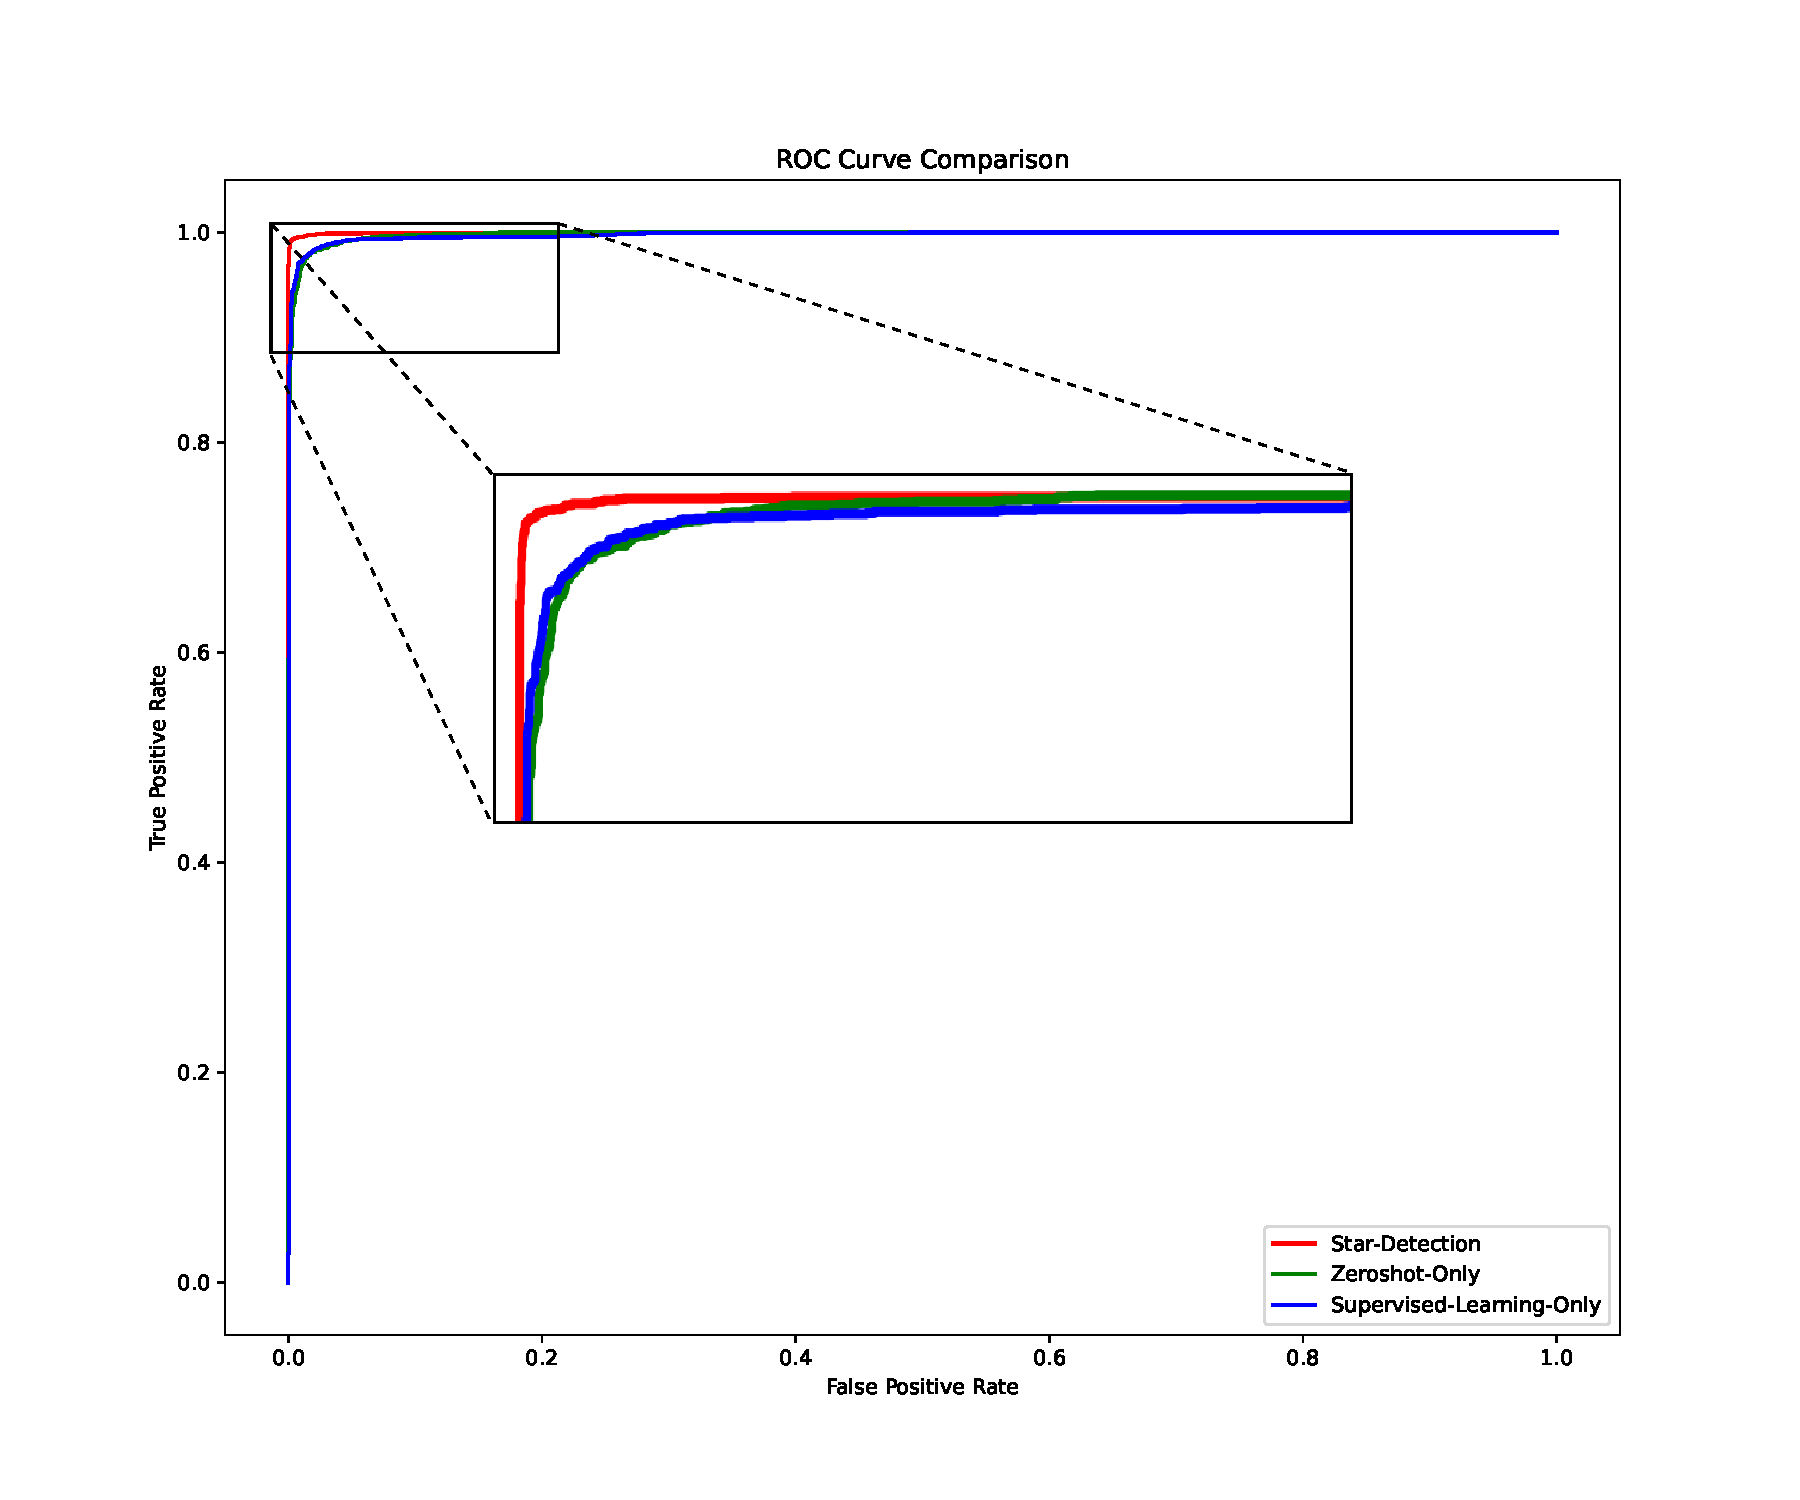
\includegraphics[width=0.95\textwidth]{figures/ROC.pdf}
	\caption{各模块ROC曲线对比图}
	\label{fig:ROC}
\end{figure}






同时,我们比较了消融实验各模块检测10000条数据需要的时间以及准确率。


\begin{table}[H]
	\centering
	\begin{tabular}{>{\centering\arraybackslash}m{4cm} >{\centering\arraybackslash}m{3cm} >{\centering\arraybackslash}m{7cm}}
		\toprule
		\textbf{模块}              & \textbf{时间/s} & \textbf{准确率} \\
		\midrule
		\multirow{1}{*}{星鉴}      & $22$          & $99.45\%$    \\
		\midrule
		\multirow{1}{*}{监督学习模块}  & $18$          & $95.77\%$    \\
		\midrule
		\multirow{1}{*}{零样本检测模块} & $121$         & $97.64\%$    \\
		\bottomrule
	\end{tabular}
	\caption{各模块检测时间及准确率}
	\label{各模块检测时间及准确率}
\end{table}











\section{多域多模型中文数据集构建及中文Benchmark的设计}
\subsection{“瀚海”多域多模型中文数据集的构建}
我们在学术与专业文献、生活与日常、新闻与媒体、艺术与文化、商业与经济等十个领域构建了不同大模型和人类文本的数据集,涵盖国内外ChatGPT,Claude3,讯飞星火,文心一言,通义千问,Kimi等主流大模型。
人类文本,我们从知网,微博,知乎,小红书等网站爬取了相关领域的内容。机器文本,则调用了ChatGPT,Claude3,讯飞星火,文心一言,通义千问,Kimi的API,将LLM的采样温度设置为0.7,所使用的提示举例如下:
%一坨屎,不知道怎么改怎么写
\begin{itemize}
	\item 请解释什么是<概念>?
	\item 请以<事物>为主题,写一首诗。
	\item 请阅读这篇文章,写一个摘要。
\end{itemize}
具体领域和数据条数如下表所示:
\begin{longtable}{|>{\centering\arraybackslash}p{0.2\textwidth}|>{\centering\arraybackslash}p{0.6\textwidth}|>{\centering\arraybackslash}p{0.05\textwidth}|}
	\hline
	\textbf{领域} & \textbf{分支}                                                                                                                            & \textbf{数量} \\ \hline
	\endfirsthead
	\multicolumn{2}{c}{(接上页)}                                                                                                                                          \\ \hline
	\textbf{领域} & \textbf{分支}                                                                                                                            & \textbf{数量} \\ \hline
	\endhead
	\multicolumn{2}{c}{(下页继续)}                                                                                                                                         \\
	\endfoot
	\endlastfoot

	学术与专业文献     & 自然科学(物理学、化学、生物学、地球科学),数学与计算机科学(数学、应用数学、计算机科学),工程与技术(机械工程、电气工程、土木工程、信息技术),社会科学(经济学、社会学、政治学),人文学科(哲学、历史学、语言学、文学),医学与健康科学(临床医学、公共卫生、医学研究) & 6128        \\ \hline
	生活与日常       & 法律咨询,医疗保健,衣食住行(美食与烹饪、家居与装修、旅行与旅游),教育与培训(学校教育、职业培训),个人理财,健康与健身                                                                          & 4912        \\ \hline
	新闻与媒体       & 国际新闻,国内新闻,财经新闻,体育新闻,娱乐新闻,科技新闻                                                                                                          & 4780        \\ \hline
	艺术与文化       & 电影与电视,音乐,戏剧,美术与设计,文化评论,历史与传统                                                                                                           & 5258        \\ \hline
	商业与经济       & 公司管理,市场营销,金融与投资,创业,供应链与物流                                                                                                              & 4997        \\ \hline
	个人创作        & 散文,小说,诗歌,博客与随笔                                                                                                                         & 4933        \\ \hline
	科技与创新       & 前沿科技,人工智能,虚拟现实,区块链                                                                                                                     & 3580        \\ \hline
	社会热点与评论     & 社会议题,政治评论,伦理讨论                                                                                                                         & 2997        \\ \hline
	娱乐与休闲       & 游戏,兴趣爱好,动漫与漫画                                                                                                                          & 3060        \\ \hline
	其他          & 笑话,公告与通知                                                                                                                               & 2882        \\ \hline
	\caption{数据集领域及话题分布}
\end{longtable}
同时为了保证数据集不同大模型的输出数据尽可能平衡,ChatGPT数据为主,其余大模型数据数量相近。
\begin{longtable}{|>{\centering\arraybackslash}p{0.17\textwidth}|>{\centering\arraybackslash}p{0.1\textwidth}|>{\centering\arraybackslash}p{0.1\textwidth}|>{\centering\arraybackslash}p{0.1\textwidth}|>{\centering\arraybackslash}p{0.1\textwidth}|>{\centering\arraybackslash}p{0.11\textwidth}|>{\centering\arraybackslash}p{0.1\textwidth}|}
	\hline
	\textbf{领域} & \textbf{ChatGPT} & \textbf{Claude3} & \textbf{讯飞星火} & \textbf{文心一言} & \textbf{通义千问} & \textbf{Kimi} \\ \hline
	\endfirsthead
	\multicolumn{5}{c}{\centering(接上页)}                                                                               \\ \hline
	\textbf{领域} & \textbf{ChatGPT} & \textbf{Claude3} & \textbf{讯飞星火} & \textbf{文心一言} & \textbf{通义千问} & \textbf{Kimi} \\ \hline
	\endhead
	\multicolumn{5}{c}{\centering(下页继续)}                                                                              \\
	\endfoot
	\endlastfoot

	学术与专业文献     & 1855             & 855              & 854           & 854           & 855           & 855           \\ \hline
	生活与日常       & 1653             & 653              & 652           & 652           & 651           & 651           \\ \hline
	新闻与媒体       & 1630             & 630              & 629           & 629           & 631           & 631           \\ \hline
	艺术与文化       & 1709             & 709              & 709           & 709           & 710           & 712           \\ \hline
	商业与经济       & 1666             & 666              & 666           & 667           & 666           & 666           \\ \hline
	个人创作        & 1655             & 655              & 656           & 656           & 655           & 656           \\ \hline
	科技与创新       & 1430             & 430              & 430           & 430           & 430           & 430           \\ \hline
	社会热点与评论     & 1333             & 333              & 333           & 333           & 332           & 333           \\ \hline
	娱乐与休闲       & 1339             & 339              & 338           & 338           & 338           & 338           \\ \hline
	其他          & 1314             & 314              & 314           & 314           & 313           & 313           \\ \hline
	\caption{数据集中不同大模型数据分配情况}
\end{longtable}
数据集的多领域以及多模型覆盖可以有效提高我们检测模型的准确率与泛化性。
\subsection{“瀚海”中文Benchmark的设计}
\begin{tcolorbox}[colback=gray!10!white, colframe=gray!50!black, title=Benchmark定义]
	Benchmark本意“基准”、“基准测试”,一种定义描述为计算机Benchmark执行一组已知的操作(测试程序),通过这些操作可以评测计算机的性能,Benchmark实际上是一个被广泛接受的、用于评估系统或模型性能的标准测试集合。
\end{tcolorbox}
在机器生成文本检测领域,Benchmark实际上就是一个分类模型在一个由人类撰写文本和机器生成文本组成的数据集上测试分类性能。在英文领域的生成文本检测Benchmark已经比较成熟,有很多公开并被广泛使用的数据集用于测试,但是中文领域的生成文本检测领域的Benchmark几乎是一片空白,因此我们在“瀚海”数据集的基础上,进一步设计并构建了“瀚海”中文Benchmark,用于中文生成文本检测模型的性能测试。

“瀚海”中文Benchmark涵盖学术,新闻,评论,诗歌,医疗,对话,动态等七个领域,包含了超过5000条中文人类撰写文本和机器生成文本的对比条目,调用了国内外一系列大模型包括ChatGPT,Claude3,讯飞星火,文心一言,通义千问,Kimi的API,采取了一系列Prompt工程进行构建。这里以新闻领域的条目构建举例:
\subsubsection{新闻领域}
\begin{enumerate}
	\item 你现在是一位文本总结大师,请根据以下内容\{human\_text\} 给出一句话总结并提取关键词, 输出到\{reponse\_text\}。
	\item 你现在是一位新闻记者,请根据以上总结和关键词\{reponse\_text\},撰写一篇新闻。
	\item 要求条理清晰逻辑严密,同时生成的文本语言人类风格明显,且不失新闻的严谨性和客观性。
\end{enumerate}

总结和撰写是两轮不同的对话,就是说大模型如果作为一名记者,他是不知道文本总结大师获得的新闻原文的,然后第三点要求是对这位新闻记者的要求,通过这样的Prompt,大模型可以生成近似人类的文本,而不是具有浓厚“AI味”的文字。
\begin{example}
	\textbf{人类文本:}新浪体育讯,北京时间8月18日,经过两轮激战,2011别克中国高尔夫球俱乐部联赛北方区复赛在天津滨海湖高尔夫俱乐部圆满落幕。会员组方面,辽宁铁岭龙山队以448杆(140-308)获得第一名,武汉天外天队以总成绩453杆(144-309)获得亚军,北辰队463杆(142-321)排名第三,这3支球队获得了北方区会员组晋级总决赛的最后3个名额。专业组方面,最终山东烟台金山队凭借4名队员的出众发挥,反超湖北红莲湖队以440杆(139-301)的成绩夺冠。湖北红莲湖队成绩也十分不错,总杆443杆(138-303)获得复赛亚军,河北石家庄世纪队447杆(141-306),这3支球队获得了北方区专业组晋级总决赛的最后3个名额。(摄影:王凌)\\
	\textbf{机器文本:} 新浪体育讯,北京时间8月18日,经过激烈的两轮比赛,2011别克中国高尔夫球俱乐部联赛北方区复赛在天津滨海湖高尔夫俱乐部圆满结束。在会员组比赛中,辽宁铁岭龙山队以448杆的成绩荣获第一名,紧随其后的是武汉天外天队,总成绩为453杆,获得亚军。北辰队则以463杆排名第三,这三支队伍成功获得了晋级总决赛的资格。在专业组方面,山东烟台金山队凭借出色的发挥,以440杆的成绩夺得冠军。湖北红莲湖队也表现出色,以总杆443杆获得复赛亚军。河北石家庄世纪队则以447杆位列第三,这三支球队同样获得了晋级总决赛的机会。此次比赛不仅展现了各队的高水平竞技能力,也为即将到来的总决赛增添了更多的悬念和期待。摄影:王凌。
\end{example}
观察这两条对比文本,如果没有标注,我们很难分辨哪一段文本由机器生成,哪一段由人类撰写,所以这是一条高质量的用于测试生成文本检测方法性能的数据。

“瀚海”中文Benchmark中绝大多数的数据都具有这样的高质量,可以作为生成文本检测方法在中文上的参考性能测试方法。


\section{基于正则表达式的文本和文件处理策略}
\subsubsection{文本分割和处理}
\paragraph{文本分割}
我们希望能够对输入的文章进行细粒度的检查,即详细的知道大语言模型生成文本在文章中的分布,这就要求我们细致的评估文章每一个部分由机器生成的概率。因此我们必须对输入的长文本进行切分,同时我们不应该破坏一个句子的完整性,所以切分出的段落应该为完整的一到几个句子,因此我们需要对匹配句子分隔符(如。?!),并将其作为标准进行段落切分。

同时考虑到对于检测来说,文本长度过短将导致其机器生成特征难以被准确检测,因此每一个部分应该有一个最低的字数限制,也就是说切分出的段落必须要语义完整且超过长度一定字数。
例如对于一段话:
\begin{example}
	不必说碧绿的菜畦,光滑的石井栏,高大的皂荚树,紫红的桑椹;也不必说鸣蝉在树叶里长吟,肥胖的黄蜂伏在菜花上,轻捷的叫天子(云雀)忽然从草间直窜向云霄里去了。单是周围的短短的泥墙根一带,就有无限趣味。油蛉在这里低唱,蟋蟀们在这里弹琴。翻开断砖来,有时会遇见蜈蚣;还有斑蝥,倘若用手指按住它的脊梁,便会拍的一声,从后窍喷出一阵烟雾。何首乌藤和木莲藤缠络着,木莲有莲房一般的果实,何首乌有拥肿的根。有人说,何首乌根是有像人形的,吃了便可以成仙,我于是常常拔它起来,牵连不断地拔起来,也曾因此弄坏了泥墙,却从来没有见过有一块根像人样。如果不怕刺,还可以摘到覆盆子,像小珊瑚珠攒成的小球,又酸又甜,色味都比桑椹要好得远。
\end{example}
处理完成之后应该变成:
\begin{example}
	\begin{itemize}
		\item 不必说碧绿的菜畦,光滑的石井栏,高大的皂荚树,紫红的桑椹;也不必说鸣蝉在树叶里长吟,肥胖的黄蜂伏在菜花上,轻捷的叫天子(云雀)忽然从草间直窜向云霄里去了。单是周围的短短的泥墙根一带,就有无限趣味。
		\item 油蛉在这里低唱,蟋蟀们在这里弹琴。翻开断砖来,有时会遇见蜈蚣;还有斑蝥,倘若用手指按住它的脊梁,便会拍的一声,从后窍喷出一阵烟雾。何首乌藤和木莲藤缠络着,木莲有莲房一般的果实,何首乌有拥肿的根。
		\item 有人说,何首乌根是有像人形的,吃了便可以成仙,我于是常常拔它起来,牵连不断地拔起来,也曾因此弄坏了泥墙,却从来没有见过有一块根像人样。如果不怕刺,还可以摘到覆盆子,像小珊瑚珠攒成的小球,又酸又甜,色味都比桑椹要好得远。
	\end{itemize}
\end{example}
\begin{algorithm}[H]
	\caption{中文文本分割}
	\begin{algorithmic}[1]
		\Procedure{SPLITT\_TEXT\_CHINESE}{text}
		\State segments $\gets$ [ ]
		\State current\_segment $\gets$
		\For{char in text}
		\State current\_segment $\gets$ current\_segment + char
		\If{len(current\_segment) $\geq$ MAXlength and char $\in$ ``。!?''}
		\State segments.append(current\_segment)
		\State current\_segment $\gets$ ``"
		\EndIf
		\EndFor
		\If{current\_segment is not empty}
		\State segments.append(current\_segment)
		\EndIf
		\State \textbf{return} segments
		\EndProcedure
	\end{algorithmic}
\end{algorithm}
\paragraph{字符筛选和剔除}
读入的文本可能会包含一些非正常字符,例如制表符,换行符,分页符以及HTML标签等,所以我们应该把这些字符给筛除掉。
对于这样的句子:
\begin{example}
	这是一个示例文本,它包含了一些需要筛除的字符,例如,{\rm HTML}标签{\rm <a>},换行符{\rm\textbackslash n},制表符{\rm\textbackslash t},还有一些英文字符ABC。
\end{example}
处理完之后应该变成:
\begin{example}
	这是一个示例文本,它包含了一些需要筛除的字符,例如{\rm HTML}标签,换行符,制表符,还有一些英文字符ABC。
\end{example}
因此在切分后的文本基础上我们需要加入对非正常字符的过滤,可以直接利用正则表达式来实现:
\begin{center}
	[\^{}{\fontspec{Consolas}\textbackslash t\textbackslash n\textbackslash f<>\textbackslash w}]
\end{center}
这样我们就能实现对非正常文本字符的筛选和剔除
\subsubsection{文件的阅读和处理}
\paragraph{不同类型文件的阅读}
PDF文件的阅读,DOCX文件的阅读和TXT文件的阅读在实现上都存在一些差异:
\begin{itemize}
	\item TXT文件是纯文本文件,读取非常简单,只需逐行读取文件内容即可。每行文本直接以字符串的形式返回,不会有额外的格式信息。
	\item PDF文件是一种页面描述语言,包含复杂的布局信息(如字体、图像、表格、注释等)。由于 PDF 文件的文本内容可能是嵌入在图像、图形对象中,或者被其他格式信息包围,所以在提取文本时可能会包含一些不必要的字符或格式信息。例如,分页符、换行符、字体样式等,都会影响提取出的文本质量。
	\item DOCX文件是一种由Microsoft Word使用的Open XML文件格式,它比TXT文件复杂,但比PDF文件容易处理。DOCX文件包含文本、段落、样式、图像、表格等结构化信息。DOCX文件的文本内容提取较为直接,但需要处理段落、页眉、页脚和其他文档元素,以确保文本的完整性和格式的保留。
\end{itemize}
因此对于不同类型的文件我们需要采用不同的方法去阅读并获得文件的内容。


\paragraph{不同类型文件的处理}
同时对不同类型的文件,我们同样需要采用不同的处理方法。PDF文件和DOCX文件包含富文本功能,因此可以直接在原文件的基础上进行标注;但是TXT文件为纯文本文件,不支持任何对字体的标注功能,因此对两大类文件我们的标注办法有所不同。

对于文件,我们需要对读进来的文本进行冗余字符的筛选和剔除,文本的分割,然后对不同的段落部分进行概率评估,最后根据文件类型和评估结果对原文件进行操作。由于我们不涉及到对DOCX文件的原始内容进行任何修改,所以DOCX文件可以直接转换为PDF文件,然后对对应的PDF文件进行操作
\begin{itemize}
	\item PDF文件\\
	      对于PDF文件,我们利用正则表达式匹配各个段落在原文件中的位置,然后根据每个段落的评估结果,对相应部分进行不同颜色的高亮标注;其中,无色表示该段文本是机器生成的概率小于15\%,黄色表示概率在15\%至84\%,红色表示概率大于84\% 。
	      我们需要同时保留过滤前后的切分文本,过滤后的文本用于进行评估,过滤前的文本用于使用正则表达式匹配原文本在文件中的位置。
	      \begin{algorithm}[H]
		      \caption{文件标注策略}
		      \begin{algorithmic}[1]
			      \Procedure{HIGHLIGHT\_DOCUMENT}{}
			      \For{$\text{page\_num} \gets 0$ \textbf{to} $\text{len(doc)}$}
			      \State $\text{page} \gets \text{doc.load\_page(page\_num)}$
			      \State $\text{text} \gets \text{page.get\_text()}$
			      \State $\text{segments} \gets \text{split\_text(text)}$
			      \State $\text{results} \gets \text{evaluate\_text\_parallel(segments)}$
			      \For{$\text{segment}, \text{(ai\_prob, human\_prob)}$ \textbf{in} $\text{zip(segments, results)}$}
			      \If{$0.15 < \text{ai\_prob} < 0.85$}
			      \State $\text{color} \gets (1, 1, 0)$ \Comment{黄色}
			      \ElsIf{$\text{ai\_prob} \geq 0.85$}
			      \State $\text{color} \gets (1, 0, 0)$ \Comment{红色}
			      \Else
			      \State \textbf{continue}
			      \EndIf
			      \State $\text{highlight\_annot} \gets \text{page.add\_highlight(segment, color)}$
			      \State $\text{highlight\_annot.update()}$
			      \EndFor
			      \EndFor
			      \EndProcedure
		      \end{algorithmic}
	      \end{algorithm}
	\item TXT文件\\
	      对于TXT文件,由于是纯文本,天生具有易于匹配对应部分位置的特点,所以可以直接根据文本搜索。对于概率评估大于10\%的部分,我们会在对应的段落前加上该段落评估的概率结果,格式如下:\par
	      [机器生成概率:$75.46\%$]\\
	      **********************************
\end{itemize}


\section{客户端实现}
\subsection{概述}
客户端采用了基于Web技术的开发框架进行开发,实现了PC端和移动端的数据访问、查询和操作界面,同时满足了跨平台用户访问的需求。UI的设计灵感主要来自于GPTzero界面以及一些开源的 Bootstrap 模板,但减少了冗余元素,力求界面简洁友好。最终实现效果如图\ref{星鉴:多域多模型的机器文本检测系统}所示。
\begin{figure}[H]
	\centering
	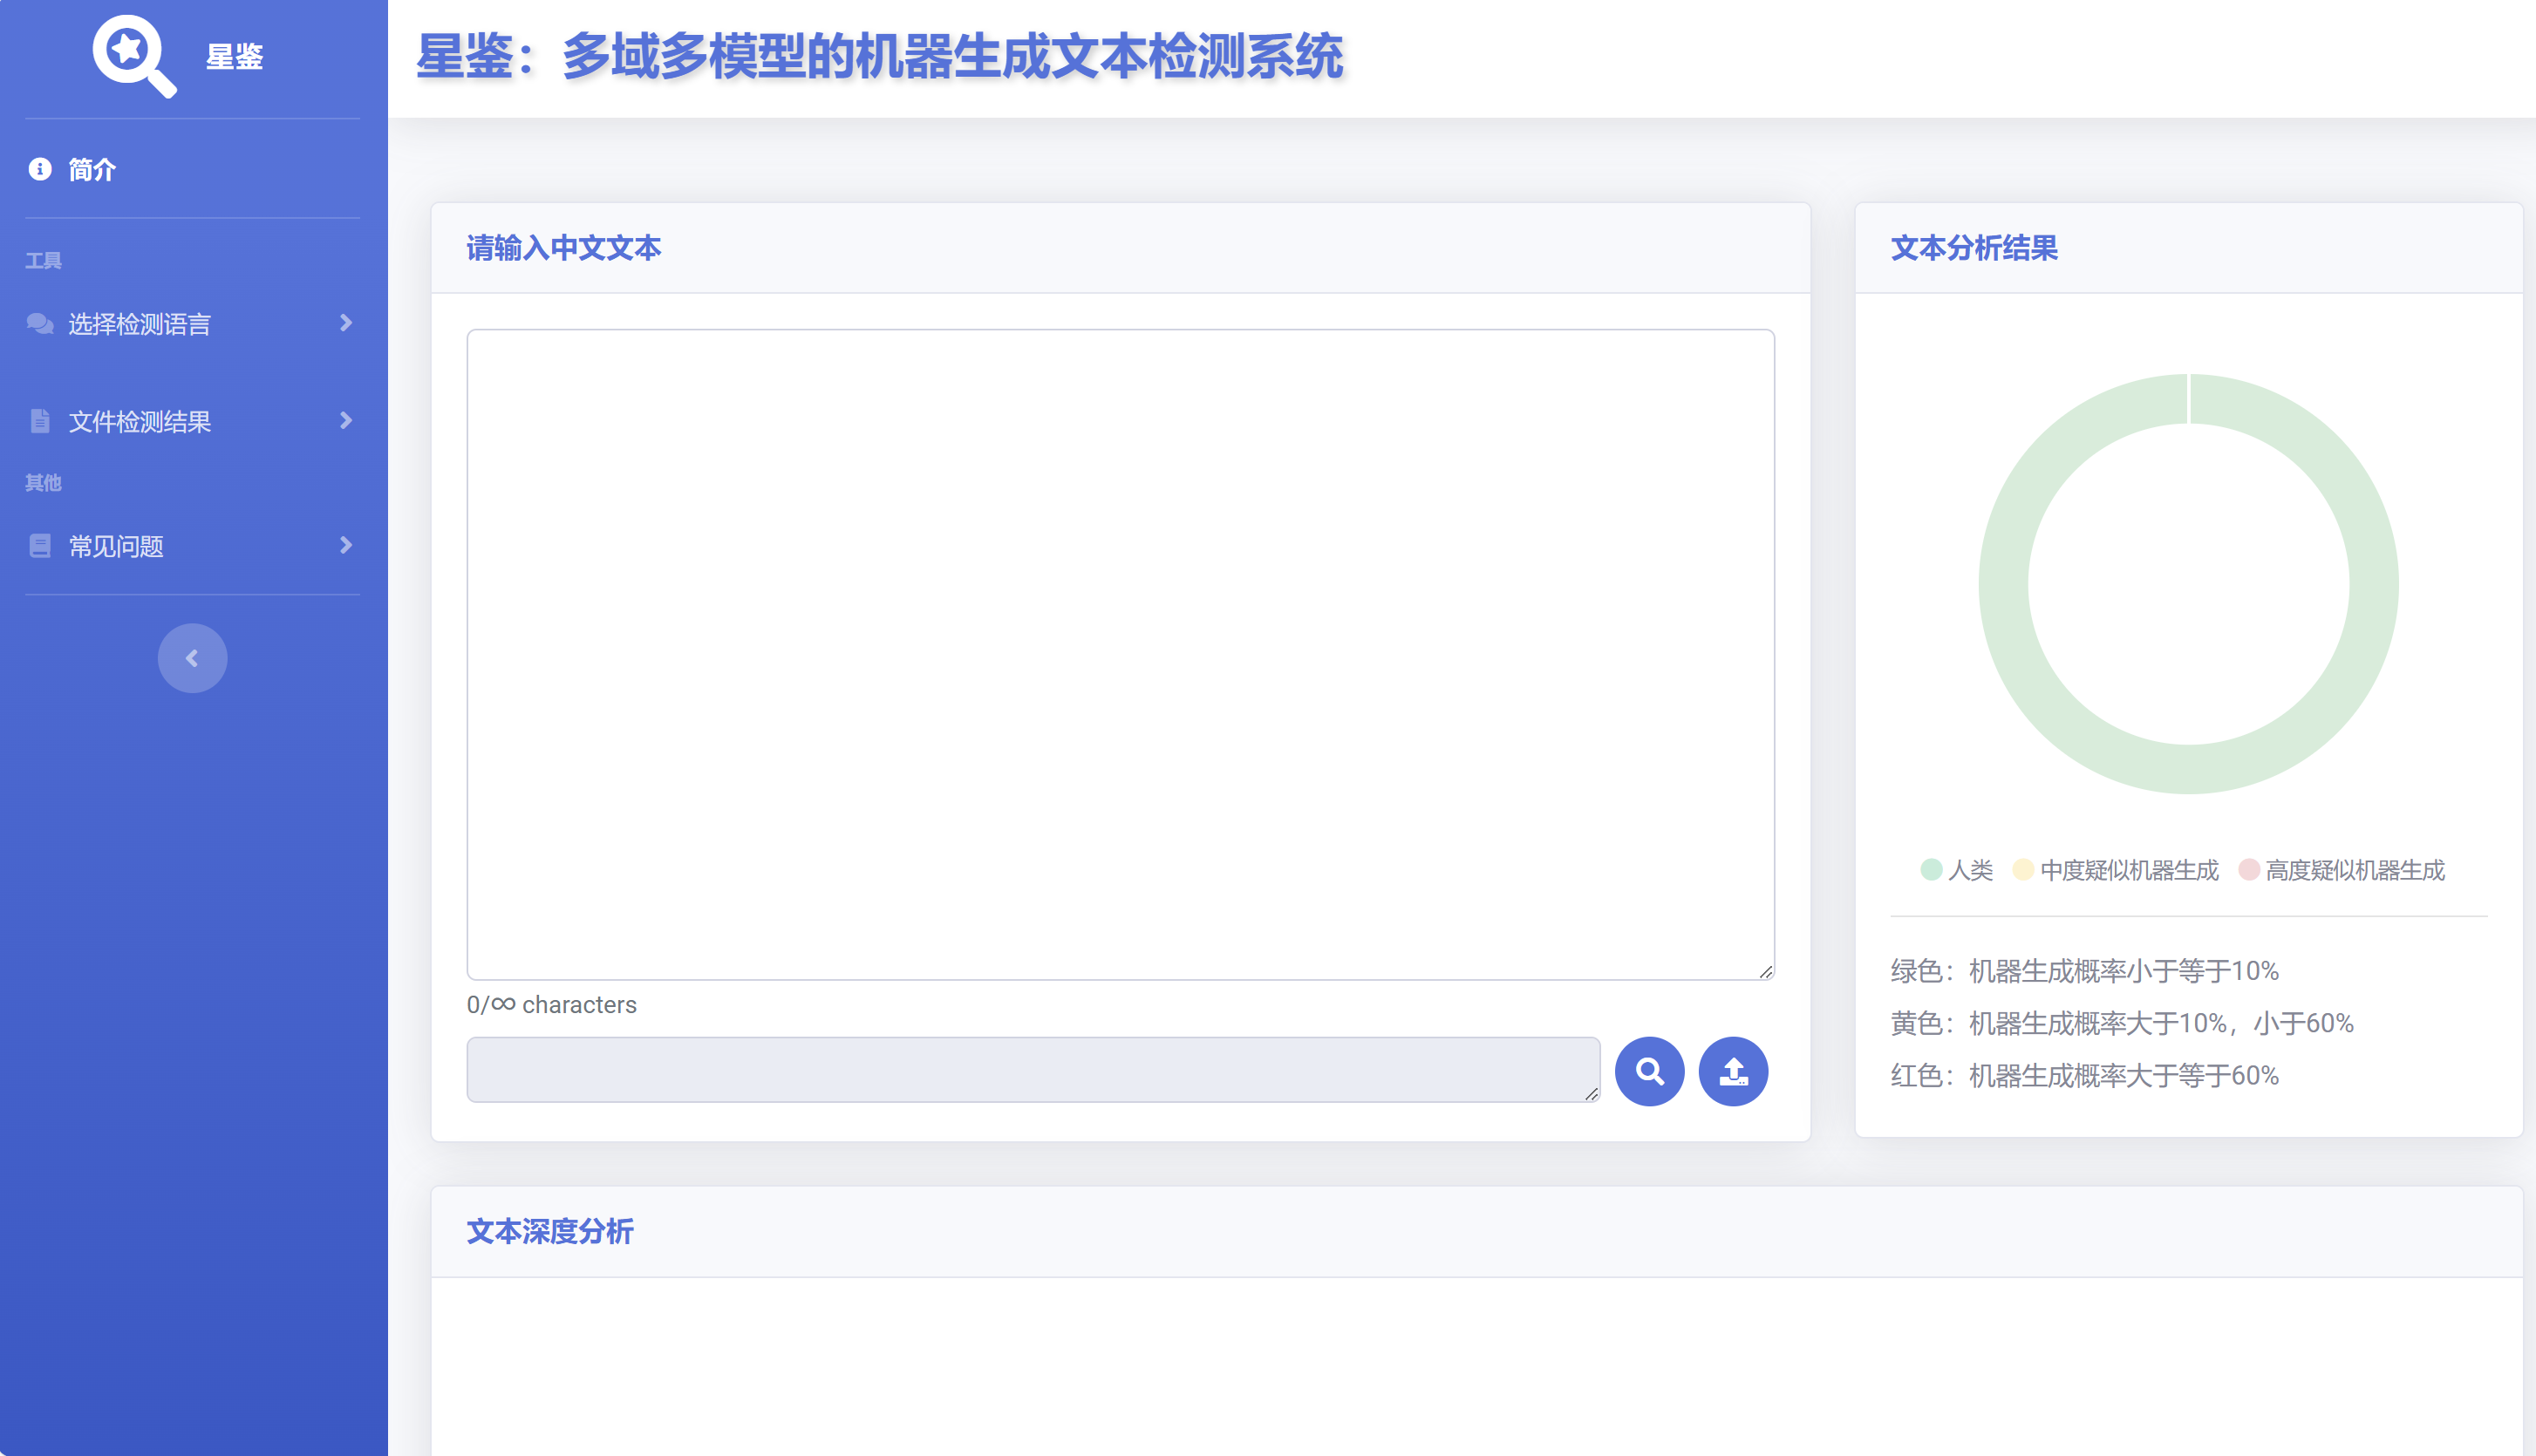
\includegraphics[width=\textwidth]{figures/系统主页.png}
	\caption{星鉴:多域多模型的机器文本检测系统}
	\label{星鉴:多域多模型的机器文本检测系统}
\end{figure}

\subsection{开发流程}
在CSS的开发中,我们主要使用了Bootstrap提供页面框架,使用了FontAwesome图标库,用于加载和使用图标,使用Google Fonts字体库,加载Nunito和Roboto字体。
\begin{enumerate}
	\item Bootstrap是由Twitter于2011年推出的一款用于前端开发的开源工具包,提供了全局的CSS设置,定义了基本的HTML元素样式和可扩展的类,同时还提供了丰富的可重用组件,如图像、下拉菜单、导航、弹出框等。Bootstrap 的特点包括响应式设计,确保网页在不同设备和屏幕尺寸下都有良好的显示效果;内置的网格系统,可以方便地进行布局设计;还有丰富的JavaScript插件,提供交互性功能。
	\item FontAwesome是一个广泛使用的图标库,它包含了数千个矢量图标,可以轻松地在网页中嵌入和使用,并支持自定义样式,可以根据需求调整大小、颜色、旋转角度等属性,满足不同的设计需求。FontAwesome 提供了各种风格的图标,包括实心、轮廓和品牌图标,适用于各种应用场景,且易于集成到任何前端框架中。值得注意的是,网页中“星鉴”的图标就是使用了FontAwesome中的放大镜和星星元素叠加来创建的。
	\item Google Fonts提供了丰富的字体选择,其字体不仅美观,还具有良好的可读性,适用于各种网页设计。Google Fonts 提供了数百种开源字体,可以通过简单的链接或 CSS 导入到网页中使用。其特点包括高性能的加载速度、跨平台的兼容性和易于实现的自定义样式,使得开发者能够轻松地为网页设计选择和应用合适的字体。
\end{enumerate}
此外,我们还参考了多个使用Bootstrap开发的开源框架,并在此基础上自定义了CSS样式,对整个UI页面进行了优化。

在JavaScript的开发组件中,我们选择通过jQuery实现动画效果,并结合Bootstrap实现了折叠等功能。其中,jQuery是一个快速、简洁的JavaScript框架,是继Prototype之后又一个优秀的JavaScript代码库(框架),于2006年1月由John Resig发布。jQuery设计的宗旨是“write Less,Do More”,即倡导写更少的代码,做更多的事情。它封装JavaScript常用的功能代码,提供一种简便的JavaScript设计模式,优化HTML文档操作、事件处理、动画设计和Ajax交互。jQuery的核心特性可以总结为:具有独特的链式语法和短小清晰的多功能接口;具有高效灵活的CSS选择器,并且可对CSS选择器进行扩展;拥有便捷的插件扩展机制和丰富的插件。jQuery兼容各种主流浏览器,如IE 6.0+、FF 1.5+、Safari 2.0+、Opera 9.0+等

在JavaScript的实现中,我们利用jQuery实现了在用户点击导航栏的链接时,显示输入文本检测区域,并根据选择的语言(中文或英文)调整输入提示和按钮行为;触发文件上传输入框,上传文件后显示检测结果;以及在文件上传和文本检测过程中显示加载指示器,并在检测完成后显示结果或错误信息。此外,为了提高用户体验,我们通过JavaScript事件处理实现了切换语言的功能。具体来说,点击中文或英文时,JavaScript代码会动态更新页面的部分内容,而不触发整个页面的刷新,避免了页面来回切换带来视觉上的割裂感。

\section{全平台应用}
在我们的设想中,星鉴应该是任何平台的用户都可以使用的,因此我们搭建了网页版的星鉴:多域多模型的机器文本检测系统,只要通过浏览器输入对应的网址就可以访问我们的检测平台。同时为了数据的隐私性,一些机密或者私密的数据并不能上传到云端处理,我们还开发了一键安装的Windows本地端,以及基于源代码运行的Linux本地端(需要用户本身有一定的技术知识)。最后考虑到Android端庞大的用户基数,我们还开发了基于云计算的安卓端应用,安装APP即可轻松使用星鉴检测系统。

\subsection{Web服务搭建}
\subsubsection{Web服务需求分析}
Web服务进行部署是星鉴系统的核心服务方式。当前,所有主流的机器文本检测工具均已开发相应的Web服务,Web服务部署具体优势如下:
\begin{itemize}
	\item \textbf{跨平台快速访问}:Web应用是当前最主流的应用程序,具有友好的访问方式。用户只需在浏览器中输入域名或IP地址,即可轻松访问相应服务。Web应用简单轻量,学习成本低,并且支持跨平台访问,使得不同操作系统的用户都可以通过浏览器访问我们的服务。此外,通过云服务和CDN(内容分发网络),Web服务可以在全球范围内快速部署和访问,为不同地区的用户提供一致的服务质量和体验。
	\item \textbf{检测方法先进}:服务器拥有强大的计算和存储资源,用户无需购买高性能硬件即可享受强大的计算和存储能力,且服务提供商能够通过集中管理和优化资源利用降低运营成本。通过在服务器上保存训练好的庞大模型,利用自身的计算能力提供快速精确的处理,星鉴可以为广大用户提供最优质的服务。这样一来,即使是没有强大计算资源的办公笔记本、手机等设备,也能使用我们最先进的方法进行检测,获得良好的检测效果。
	\item \textbf{可扩展性强}: Web服务可以根据需求进行扩展,通过增加服务器和负载均衡器,可以应对大量并发请求,确保服务的稳定性和可用性。
	\item \textbf{易于维护和更新}: Web服务的集中管理使得维护和更新更加便捷。服务器上的更新可以即时推送到所有用户,无需用户手动更新,从而确保用户始终使用最新的功能和安全补丁。此外,Web服务可以不断进行实时监控和数据收集,帮助开发团队快速发现问题和改进服务。通过分析用户行为和反馈,能够及时进行优化和更新,提升用户体验。
\end{itemize}

\subsubsection{服务器部署流程}
考虑到开发成本以及访问速度,我们最终以单服务器架构进行部署。因时间有限,星鉴系统未部署数据库系统,所有文件数据保存在服务器本地。因成本有限,我们最终采用云服务器按量计费模式部署服务,由于按量计费不支持域名绑定服务(需要购买服务器时间超过3个月才能绑定域名),星鉴无法申请SSL证书,使用HTTPS加密通信,并利用HTTP/2进一步加速服务。上述问题我们将在后续进一步改进,使星鉴的服务更加安全与完善。

星鉴的云服务器配置信息请见4.1小节。

Web服务由Nginx提供,其中Nginx在Web服务中具有卓越的性能、灵活性和安全性,是企业和开发者提供高效Web服务的理想选择。最终服务器监听80端口,收到请求后将会返回页面给用户,用户点击检测后请求将会传到服务器对应的5000端口并进行进一步交互。

最终我们开发了两个前端页面,分别对应电脑和手机访问,服务器访问index.html后会自动识别跳转,具体页面展示可见3.6小节的使用说明。

\subsection{Windows本地端开发}
\subsubsection{本地端需求分析}
本地端开发是星鉴系统的重要组成部分,可以满足用户多方面的需求。
\begin{itemize}
	\item \textbf{保护数据隐私}:在某些场景中,用户的数据具有高度的敏感性,不适合上传到云端进行处理。通过开发本地端应用,用户可以在本地环境中完成数据分析与检测,确保数据的隐私和安全。
	\item \textbf{利用本地算力}:网页端平台的算力有限,如果短时间内有大量用户访问,很难迅速地提供检测结果,本地端应用,用户可以充分利用本地地算力,及时高效的提供检测结果。
	\item \textbf{实现离线使用}:在某些网络连接不稳定或者不允许和外界有网络连接的离线场景,本地端应用给用户提供了无需连接网络即可使用星鉴系统的选择。
\end{itemize}

\subsubsection{本地端开发流程}
本地端应用的架构和网页端服务器架构近似相同,但是UI是基于本地渲染,无需调用浏览器进行查看;且本地端的检测方法和网页端相同,但是使用参数更小的预训练模型,同时考虑到用户计算机中可能并未包含阅读检测文件的软件,还实现了一个文件阅读器。

为了全平台的UI统一且采用统一的操作逻辑,本地端的交互UI界面,基于\textbf{Pyside6}框架开发,借助内嵌一个\textbf{微型浏览器内核},实现HTML内容的渲染,并借助对应页面实现用户交互逻辑的实现。
\tikzstyle{block} = [rectangle, draw, fill=blue!20, text centered, rounded corners, minimum height=3em]
\tikzstyle{line} = [draw, -latex']
\tikzstyle{techdetail} = [rectangle, draw, fill=yellow!30, text centered, minimum height=1cm, minimum width=3cm]

\begin{figure}[H]
	\centering
	\begin{tikzpicture}[node distance=2cm, auto]

		% UI Module
		\node [block] (submission) {用户提交文本/文件};
		\node [block, left of=submission, xshift=-3cm] (displayresult) {显示结果};

		% Draw box around UI Module
		\node [draw, dashed, fit=(submission) (displayresult), inner sep=0.75cm, label=above:UI模块] (uibox) {};

		% Preprocessing block
		\node [block, below of=submission] (preprocessing) {预处理};

		% File/Text Processing Module
		\node [block, below left of=preprocessing, xshift=-3cm] (fileprocessing) {内容读取和切分};
		\node [block, below of=fileprocessing] (filter) {筛除字符};
		\node [block, below of=filter] (mark) {文件标注};
		\node [block, below of=mark] (report){生成报告};

		% File/Text Processing Module - outer box
		\node [draw, dashed, fit=(fileprocessing) (filter) (mark)(report), inner sep=0.75cm, label=above:文本/文件处理模块] (processingbox) {};

		% Model Module
		\node [block, below right of=preprocessing, xshift=3cm] (model) {监督学习检测方法};
		\node [block, below of=model] (Zeroshot) {Zero-Shot检测方法};
		\node [block, below of=Zeroshot] (evaluation) {融合判据综合评估};

		% Model Module - outer box
		\node [draw, dashed, fit=(model) (Zeroshot) (evaluation), inner sep=0.75cm, label=above:分类模块] (modelbox) {};

		% Draw edges
		\path [line] (submission) -- (preprocessing);
		\path [line] (preprocessing) -- (fileprocessing);
		\path [line] (fileprocessing) -- (filter);
		\path [line] (filter) -- (mark);
		\path [line] (filter) -- (Zeroshot);
		\path [line] (filter.east) -| ([xshift=3cm]filter.east) |- (model.west);
		\path [line] (report) -- ++(-2,0) |- (displayresult);
		\path [line] (model.east) |- ++(0.5,0) |- (evaluation.east);
		\path [line] (Zeroshot) -- (evaluation);
		\path [line] (evaluation) -- (mark) node[midway, above] {返回评估结果};
		\path[line](mark)--(report);
	\end{tikzpicture}
	\caption{星鉴本地端应用架构图}
\end{figure}
同时我们希望实现Windows端的应用可以打包成一个直接可以安装的安装包,用户下载点击之后就可以一键安装,安装完成之后即可开始使用。

源代码是需要基于Python环境运行的,如果用户电脑中没有安装Python以及对应的模块,那么基于源代码是无法运行的。Windows操作系统中最常见的可执行文件格式为.exe格式,因此一般一个可以直接运行的程序都是以.exe的形式存在的。

\textbf{PyInstaller}是一个非常受欢迎和强大的工具,它可以将 Python程序转换成独立的可执行文件,适用于 Windows、Linux 和 macOS 系统,所以我们可以直接利用\textbf{Pyinstaller}将Python源代码.py格式打包成Windows操作系统下的可执行文件.exe格式。\textbf{PyInstaller}会把运行应用的所有依赖都打包成一个exe文件(或者一个exe文件加上依赖的文件夹)。

获得了Windows下的可执行程序之后,我们还需要将可执行程序以及运行所依赖的一些文件一起打包成一个安装程序,这样用户只需要下载这个安装程序,就直接直接点击一键安装。我们采用了\textbf{Inno Setup}工具,\textbf{Inno Setup}是一款Windows免费的安装制作软件,可以把一个可执行程序以及对应的一些文件打包并制作成一个安装程序,同时提供一些预设(例如选择安装路径,选择为哪些用户安装等)可供选择。最终打包安装包如下图所示:
\begin{figure}[H]
	\centering
	\includegraphics[width=\textwidth]{figures/星鉴安装程序.png}
	\caption{星鉴安装程序}
\end{figure}
按照安装程序的指引一步一步走,最后就可以获得一个在本地原生运行的星鉴机器生成文本检测系统。
\subsection{Android端开发}
\subsubsection{Android端需求分析}
Android端星鉴应用开发具有着重大意义:
\begin{itemize}
	\item \textbf{市场覆盖}:Android是全球最普及的移动设备操作系统,拥有庞大的用户基础。开发Android端应用可以覆盖更多用户,让更多人方便地使用星鉴系统。
	\item \textbf{移动便捷}:相比桌面端,移动端设备更便于携带和随时随地使用,用户可以在任何时间、任何地点进行文本检测,提升了系统的可访问性。
	\item \textbf{使用方便}:由于当前移动设备普及的触摸逻辑,星鉴应用学习成本极低,交互逻辑友好,零技术基础的用户也可以轻松上手使用。
\end{itemize}

有了Android端应用,一名教师可以随时检测他的学生手写的文章,一名社区内容审核员可以在任何时间任何地点对社区中大量的机器人言论进行检测管控,一位只会使用微信这类应用的老年人也可以面对一些由机器生成的诈骗信息有更简单和更方便的防范措施。
\subsubsection{Android端开发流程}
由于移动设备本身的算力限制,在本地原生计算是不太现实的,因此本地应用渲染UI和用户交互,然后云端进行计算并返回检测结果的设计是更加合理的。因此我们开发的安卓应用逻辑如下:
\begin{figure}[H]
	\centering
	\resizebox{0.7\textwidth}{!}{ % 调整这个参数以改变图片大小
		\begin{tikzpicture}[node distance=2cm]
			\tikzstyle{startstop} = [rectangle, rounded corners, minimum width=3cm, minimum height=1cm,text centered, draw=black, fill=red!30]
			\tikzstyle{process} = [rectangle, minimum width=3cm, minimum height=1cm, text centered, draw=black, fill=orange!30]
			\tikzstyle{arrow} = [thick,->,>=stealth]
			\tikzstyle{entity} = [text centered, draw=black, minimum height=2cm]

			\node (user) [entity, minimum height=8cm, minimum width=4cm, label=above:用户] {};
			\node (cloud) [entity, right of=user, xshift=6cm, minimum height=8cm, minimum width=4cm, label=above:云端] {};

			\node (start) [startstop, below of=user, yshift=3cm] {用户启动安卓应用};
			\node (upload) [process, below of=start] {输入文本或上传文件};
			\node (cloudcalc) [process, below of=cloud, yshift=3cm] {对上传内容进行检测};
			\node (result) [process, below of=cloudcalc] {返回检测结果};
			\node (end) [startstop, below of=upload] {显示结果};

			\draw [arrow] (start) -- (upload);
			\draw [arrow] (upload.east) -- ++(1,0) |- (cloudcalc.west);
			\draw [arrow] (cloudcalc) -- (result);
			\draw [arrow] (result.west) -- ++(-1,0) |- (end);

		\end{tikzpicture}
	} % 调整这个参数以改变图片大小
	\caption{星鉴Android端应用逻辑示意图}
\end{figure}
最后实现的效果如下图所示:
\begin{figure}[H]
	\centering
	\includegraphics[width=0.8\textwidth]{figures/Android.png}
	\caption{星鉴Android端展示}
	\label{星鉴Android端展示}
\end{figure}
\section{使用说明}
星鉴:多域多模型的机器文本检测系统全平台采用同一套操作逻辑,因此使用方法完全相同,检测功能主要分为文本检测和文件检测两种。
\subsection{文本检测}
用户可以直接在网页端,输入一段文本,然后检测这段文本是否由机器生成以及这段文本有哪些部分由机器生成。文本输入不设上限。

先点击输入文本检测,然后选择中文(英文功能还在测试中),随后在出现的文本框中输入一段文字,最后点击右下角的按钮,便可以检测这段文字是否由机器生成。
\begin{figure}[H]
	\centering
	\begin{subfigure}[b]{0.45\textwidth}
		\centering
		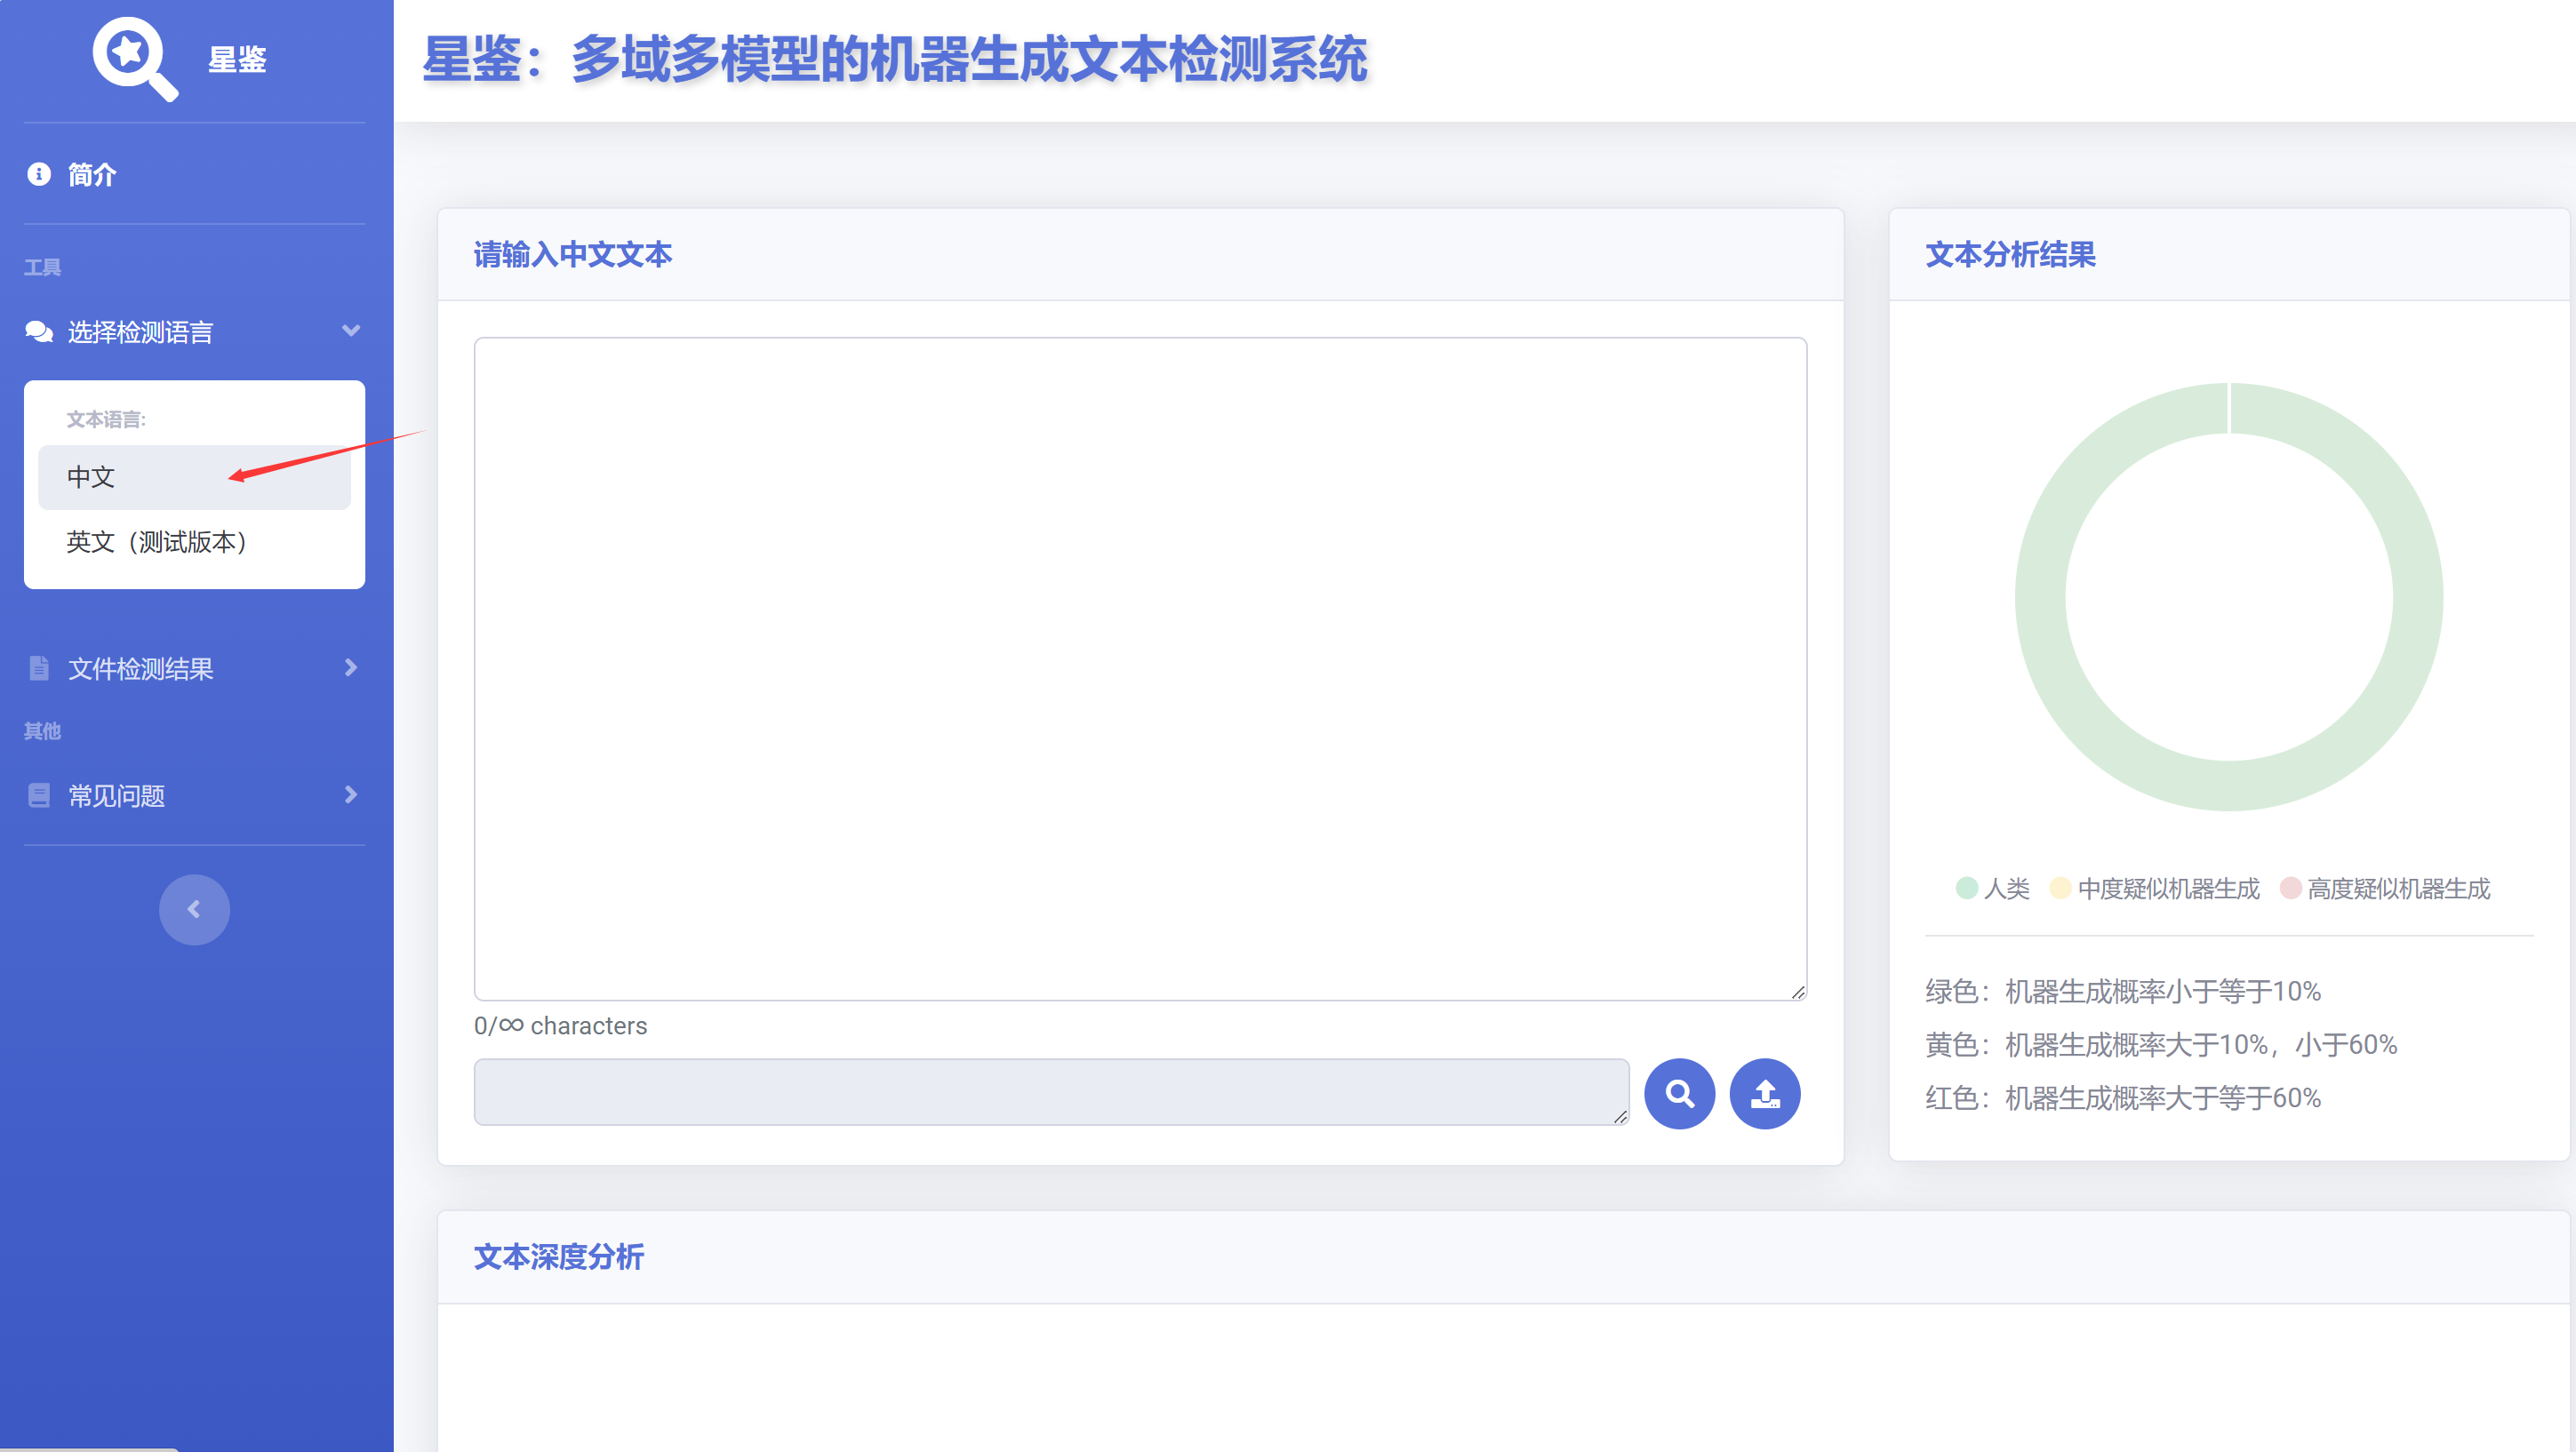
\includegraphics[width=\textwidth]{figures/选择中文检测.png}
		\caption{选择中文检测功能}
		\label{选择中文检测功能}
	\end{subfigure}
	\begin{subfigure}[b]{0.47\textwidth}
		\centering
		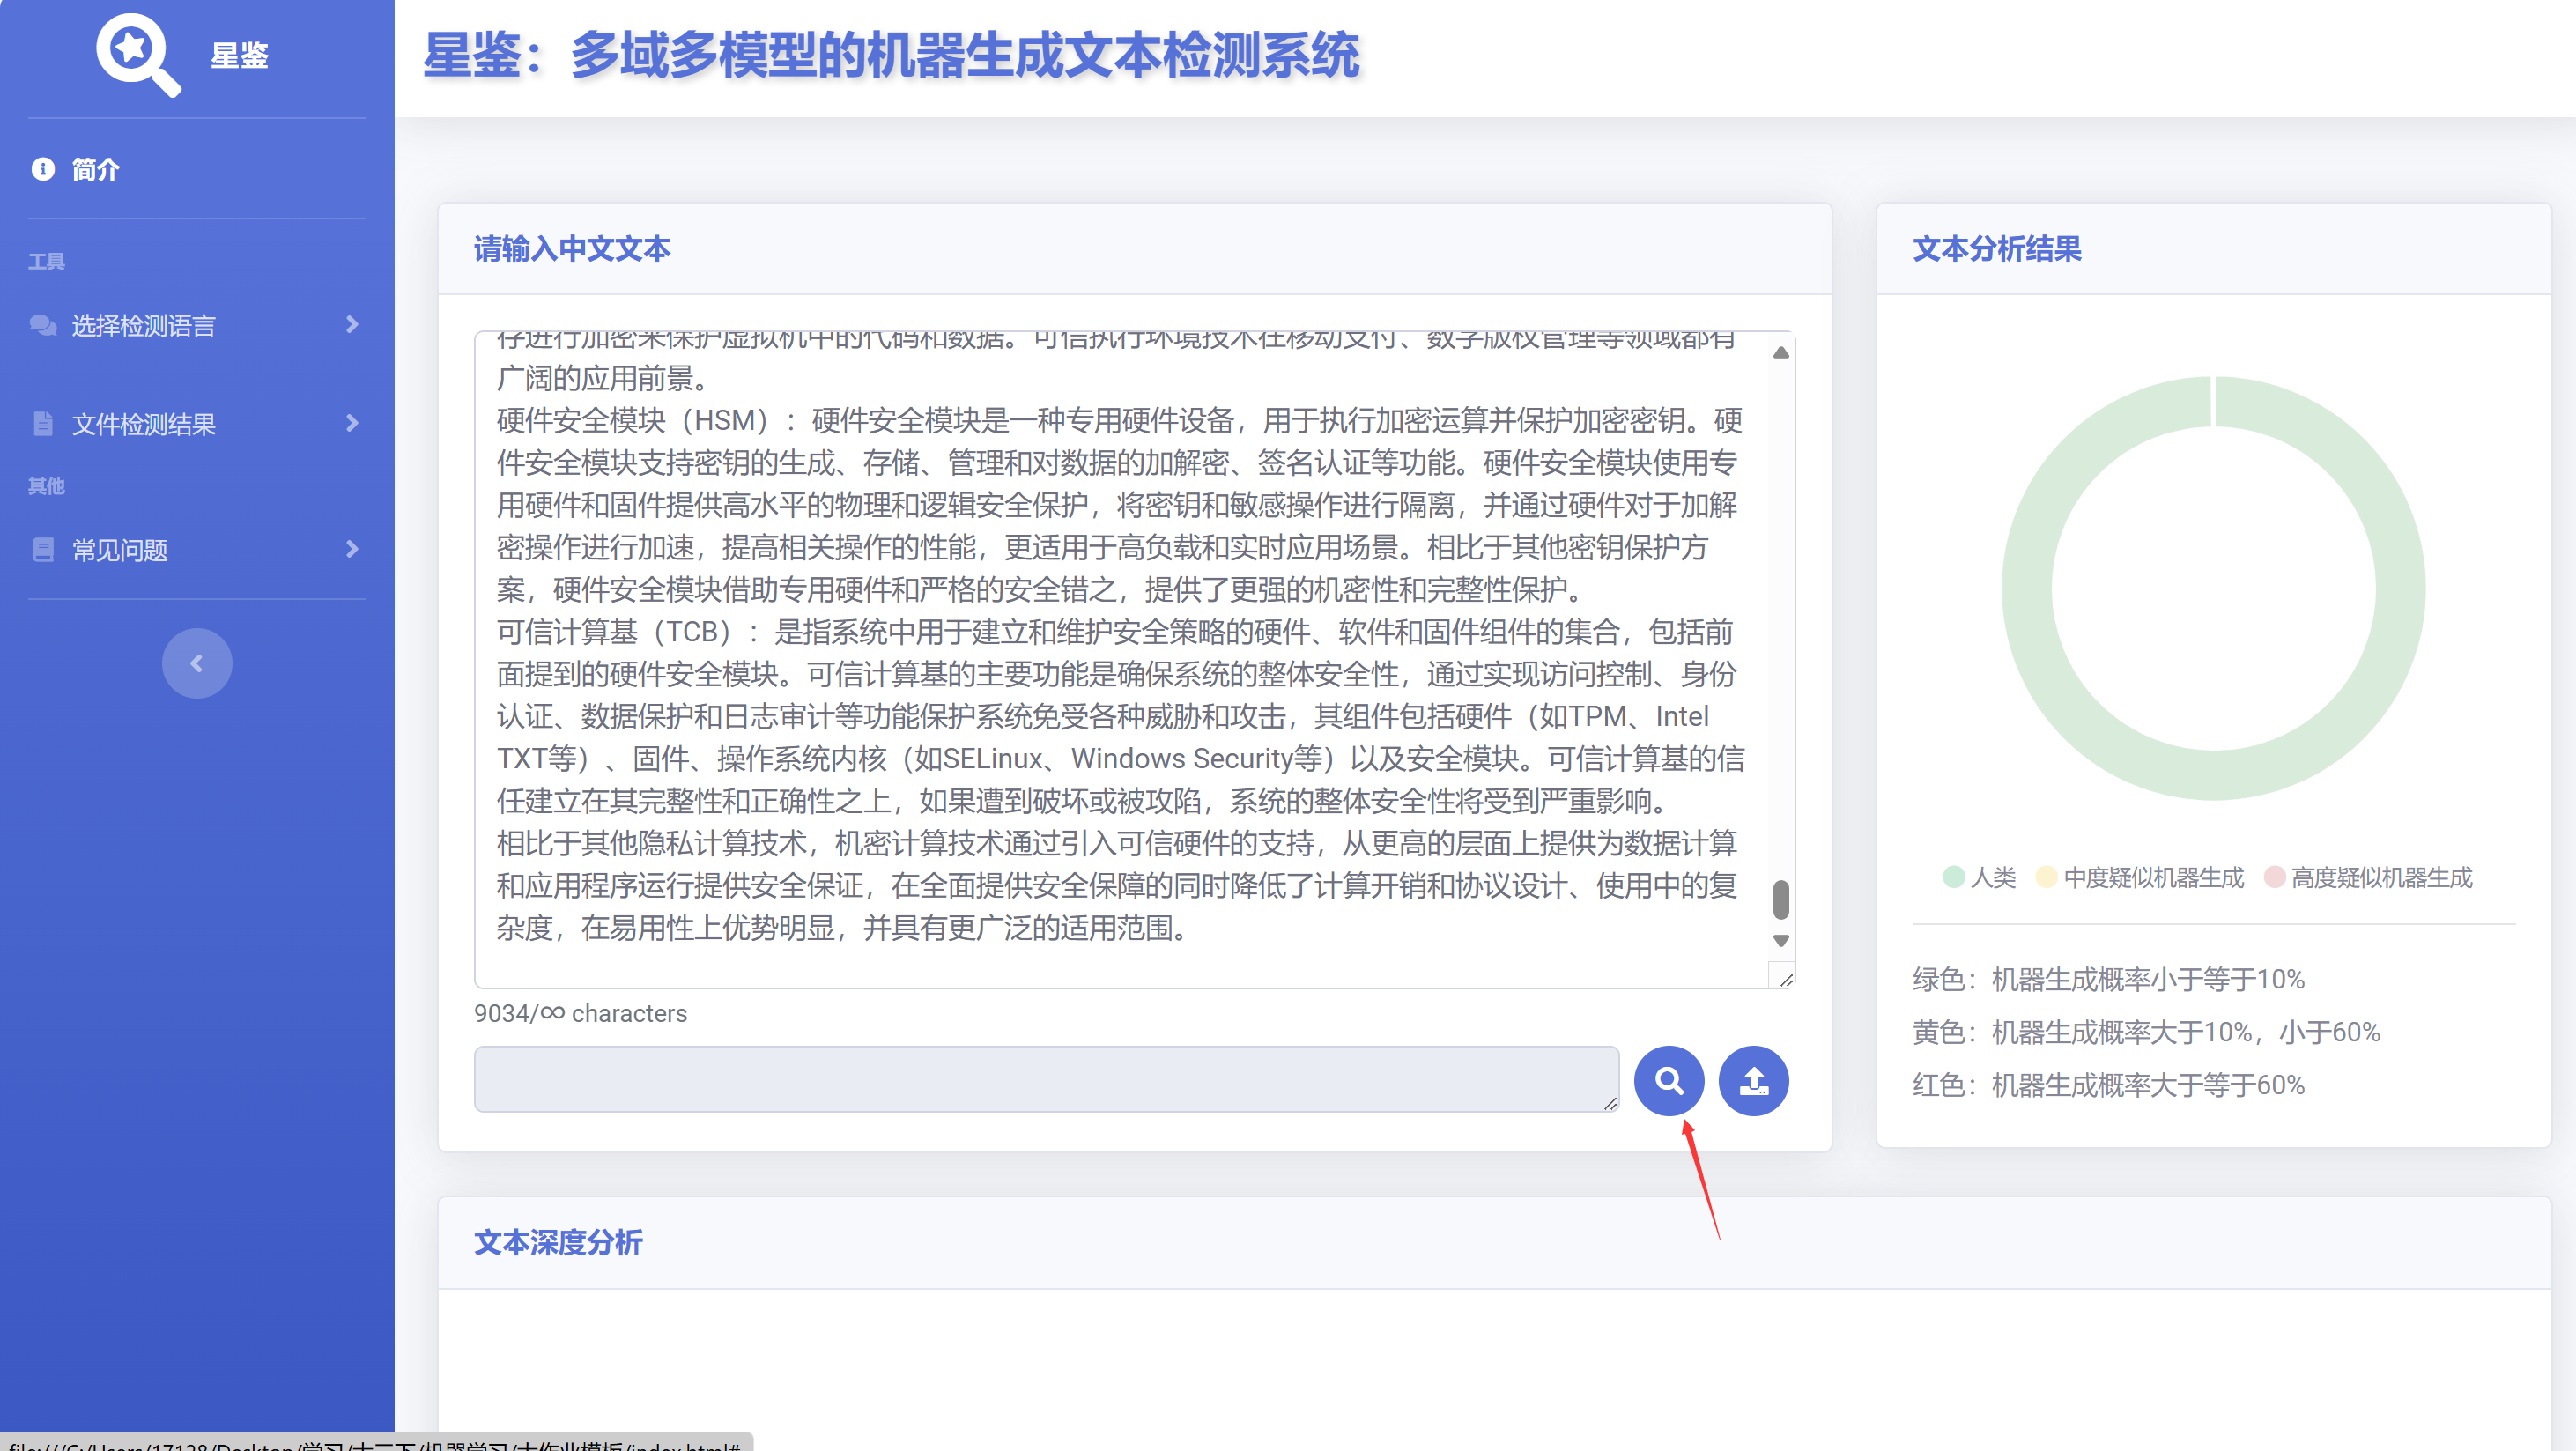
\includegraphics[width=\textwidth]{figures/输入文本检测.png}
		\caption{输入文本进行检测}
		\label{输入文本进行检测}
	\end{subfigure}
	\caption{中文文本检测流程}
	\label{中文文本检测流程}
\end{figure}
检测完成之后,会告知用户这段文本总体由机器生成的综合指数,并展示人类文本,中度疑似机器生成文本以及高度疑似机器生成文本在文本中的比例。瓶状图中三种颜色绿,黄,红,代表不同的文本成分,分别为人类生成,中度疑似机器生成和高度疑似机器生成。
\begin{figure}[H]
	\centering
	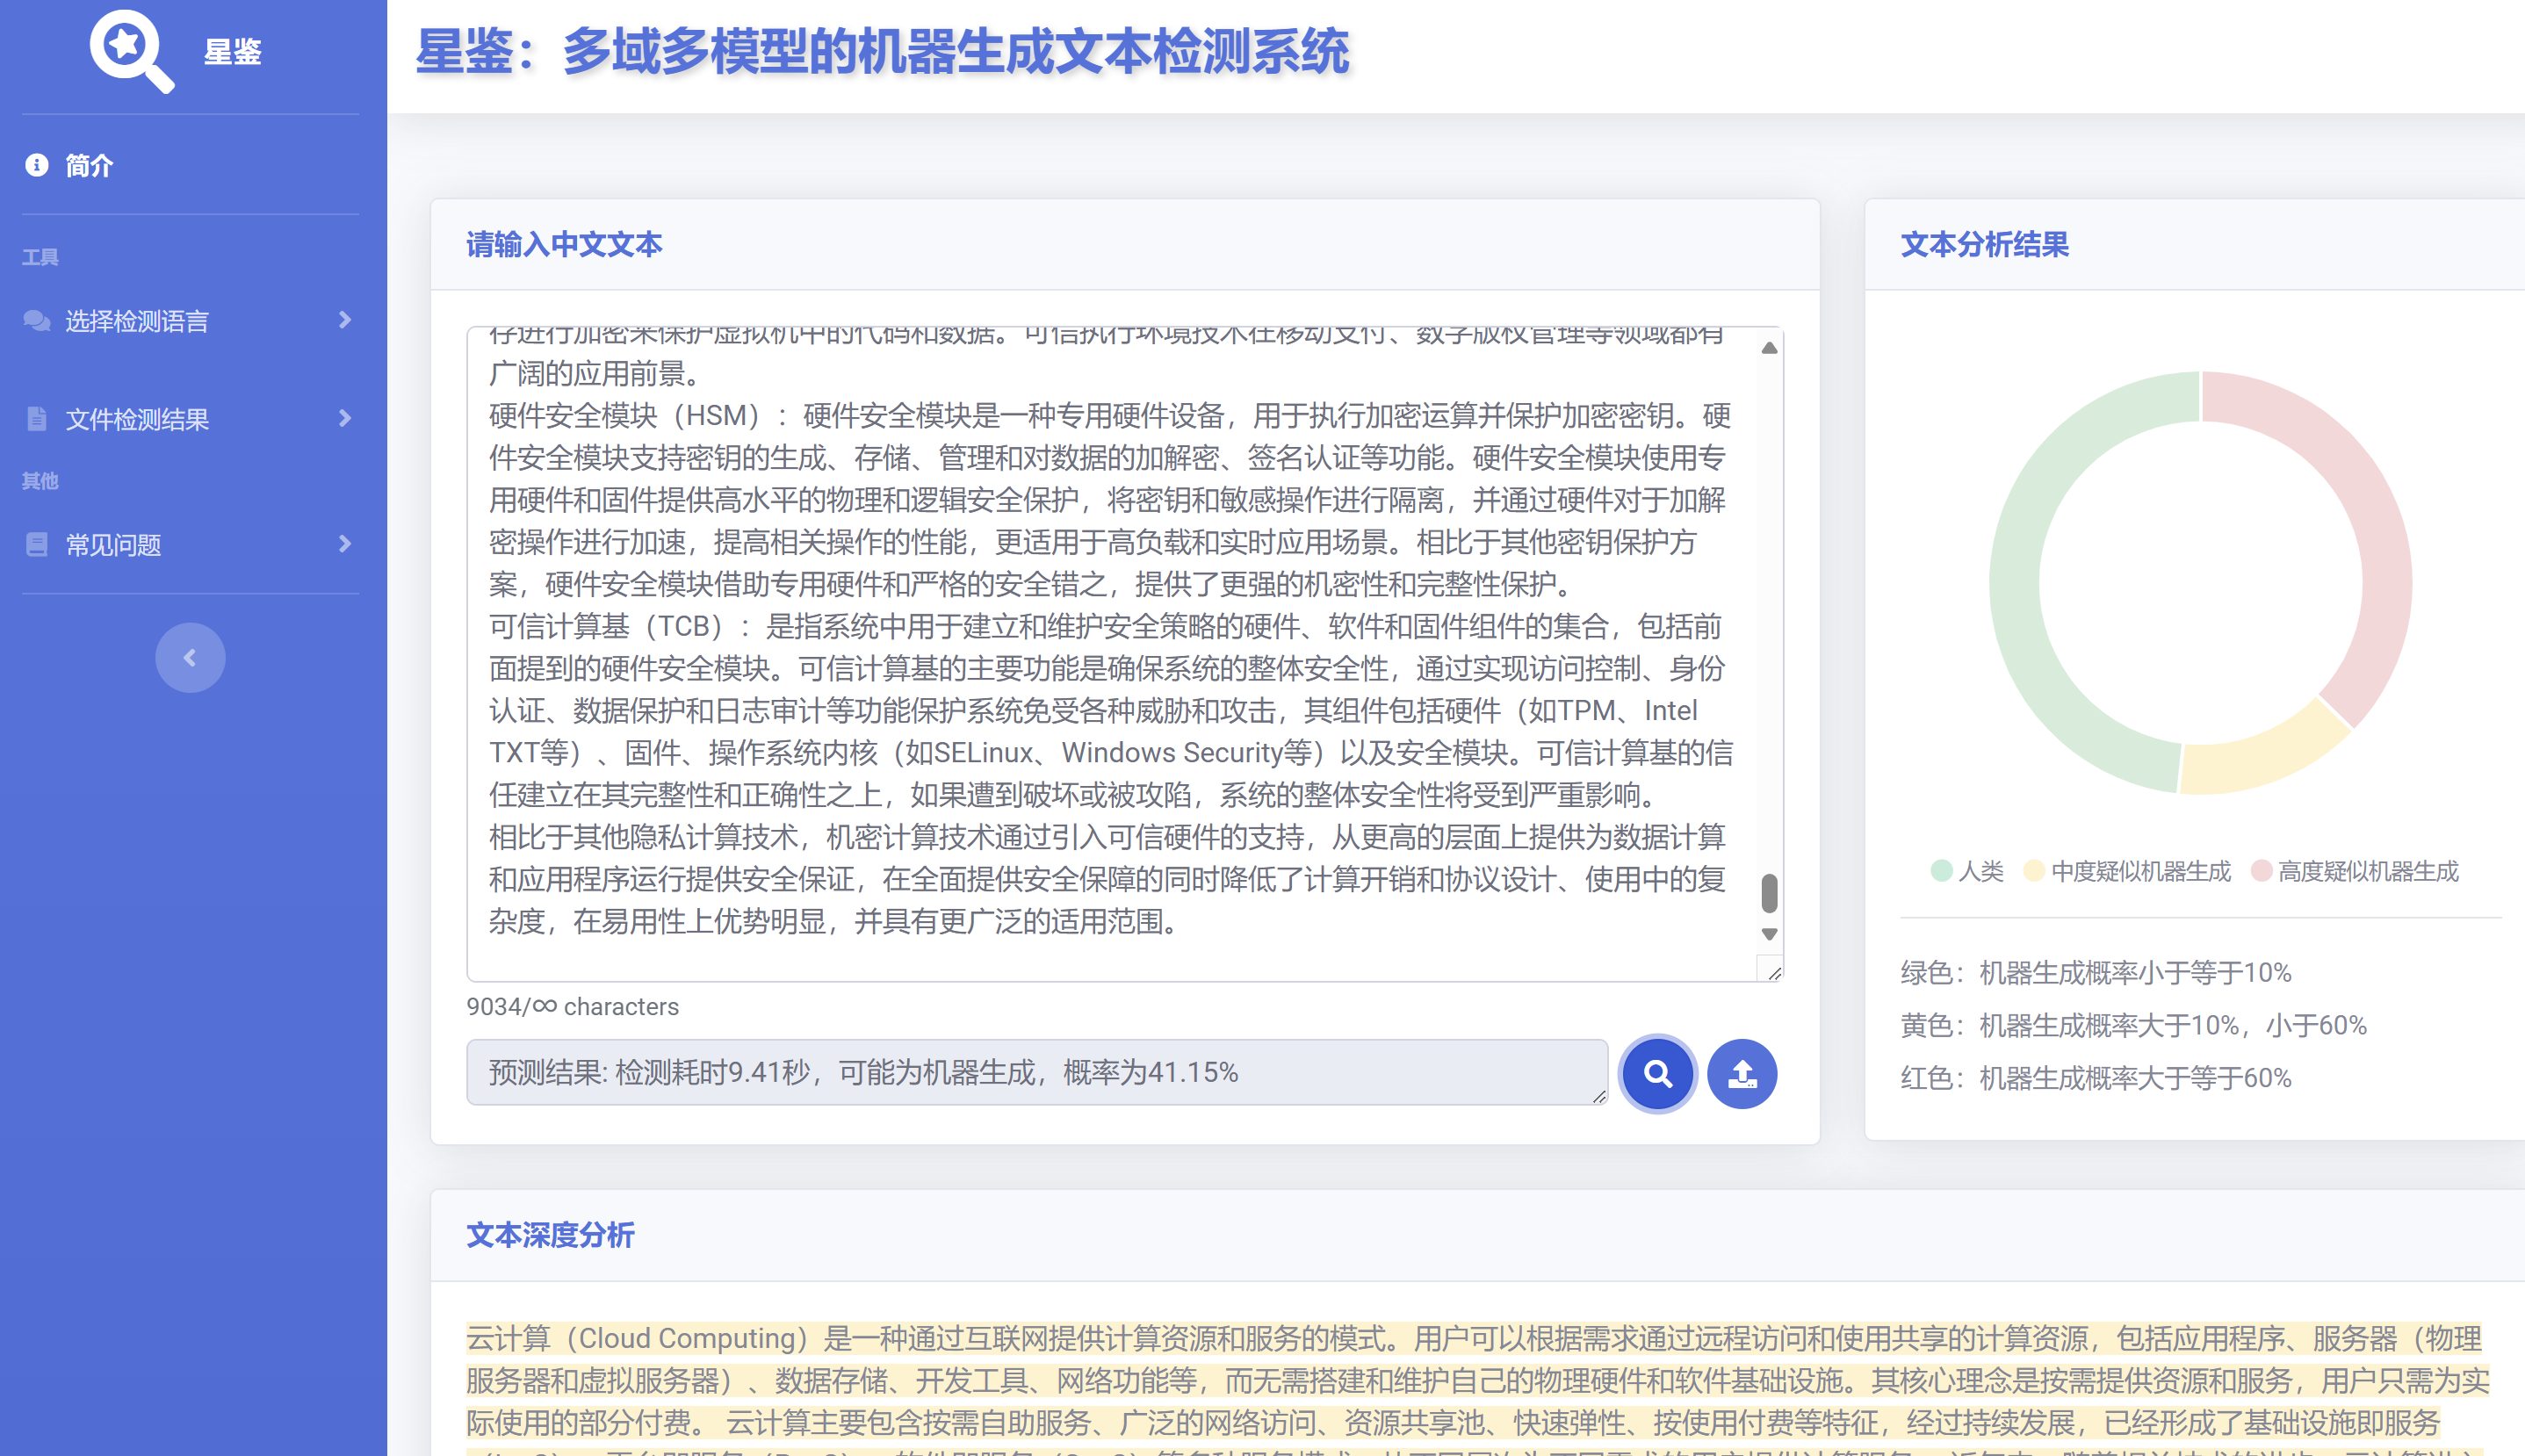
\includegraphics[width=\textwidth]{figures/文本检测结果.png}
	\caption{初步检测结果}
	\label{初步检测结果}
\end{figure}
在文本的深度分析中,会告知用户不同部分由机器生成的概率大小,文本的标注颜色代表这不同部分的文本成分。
\begin{figure}[H]
	\centering
	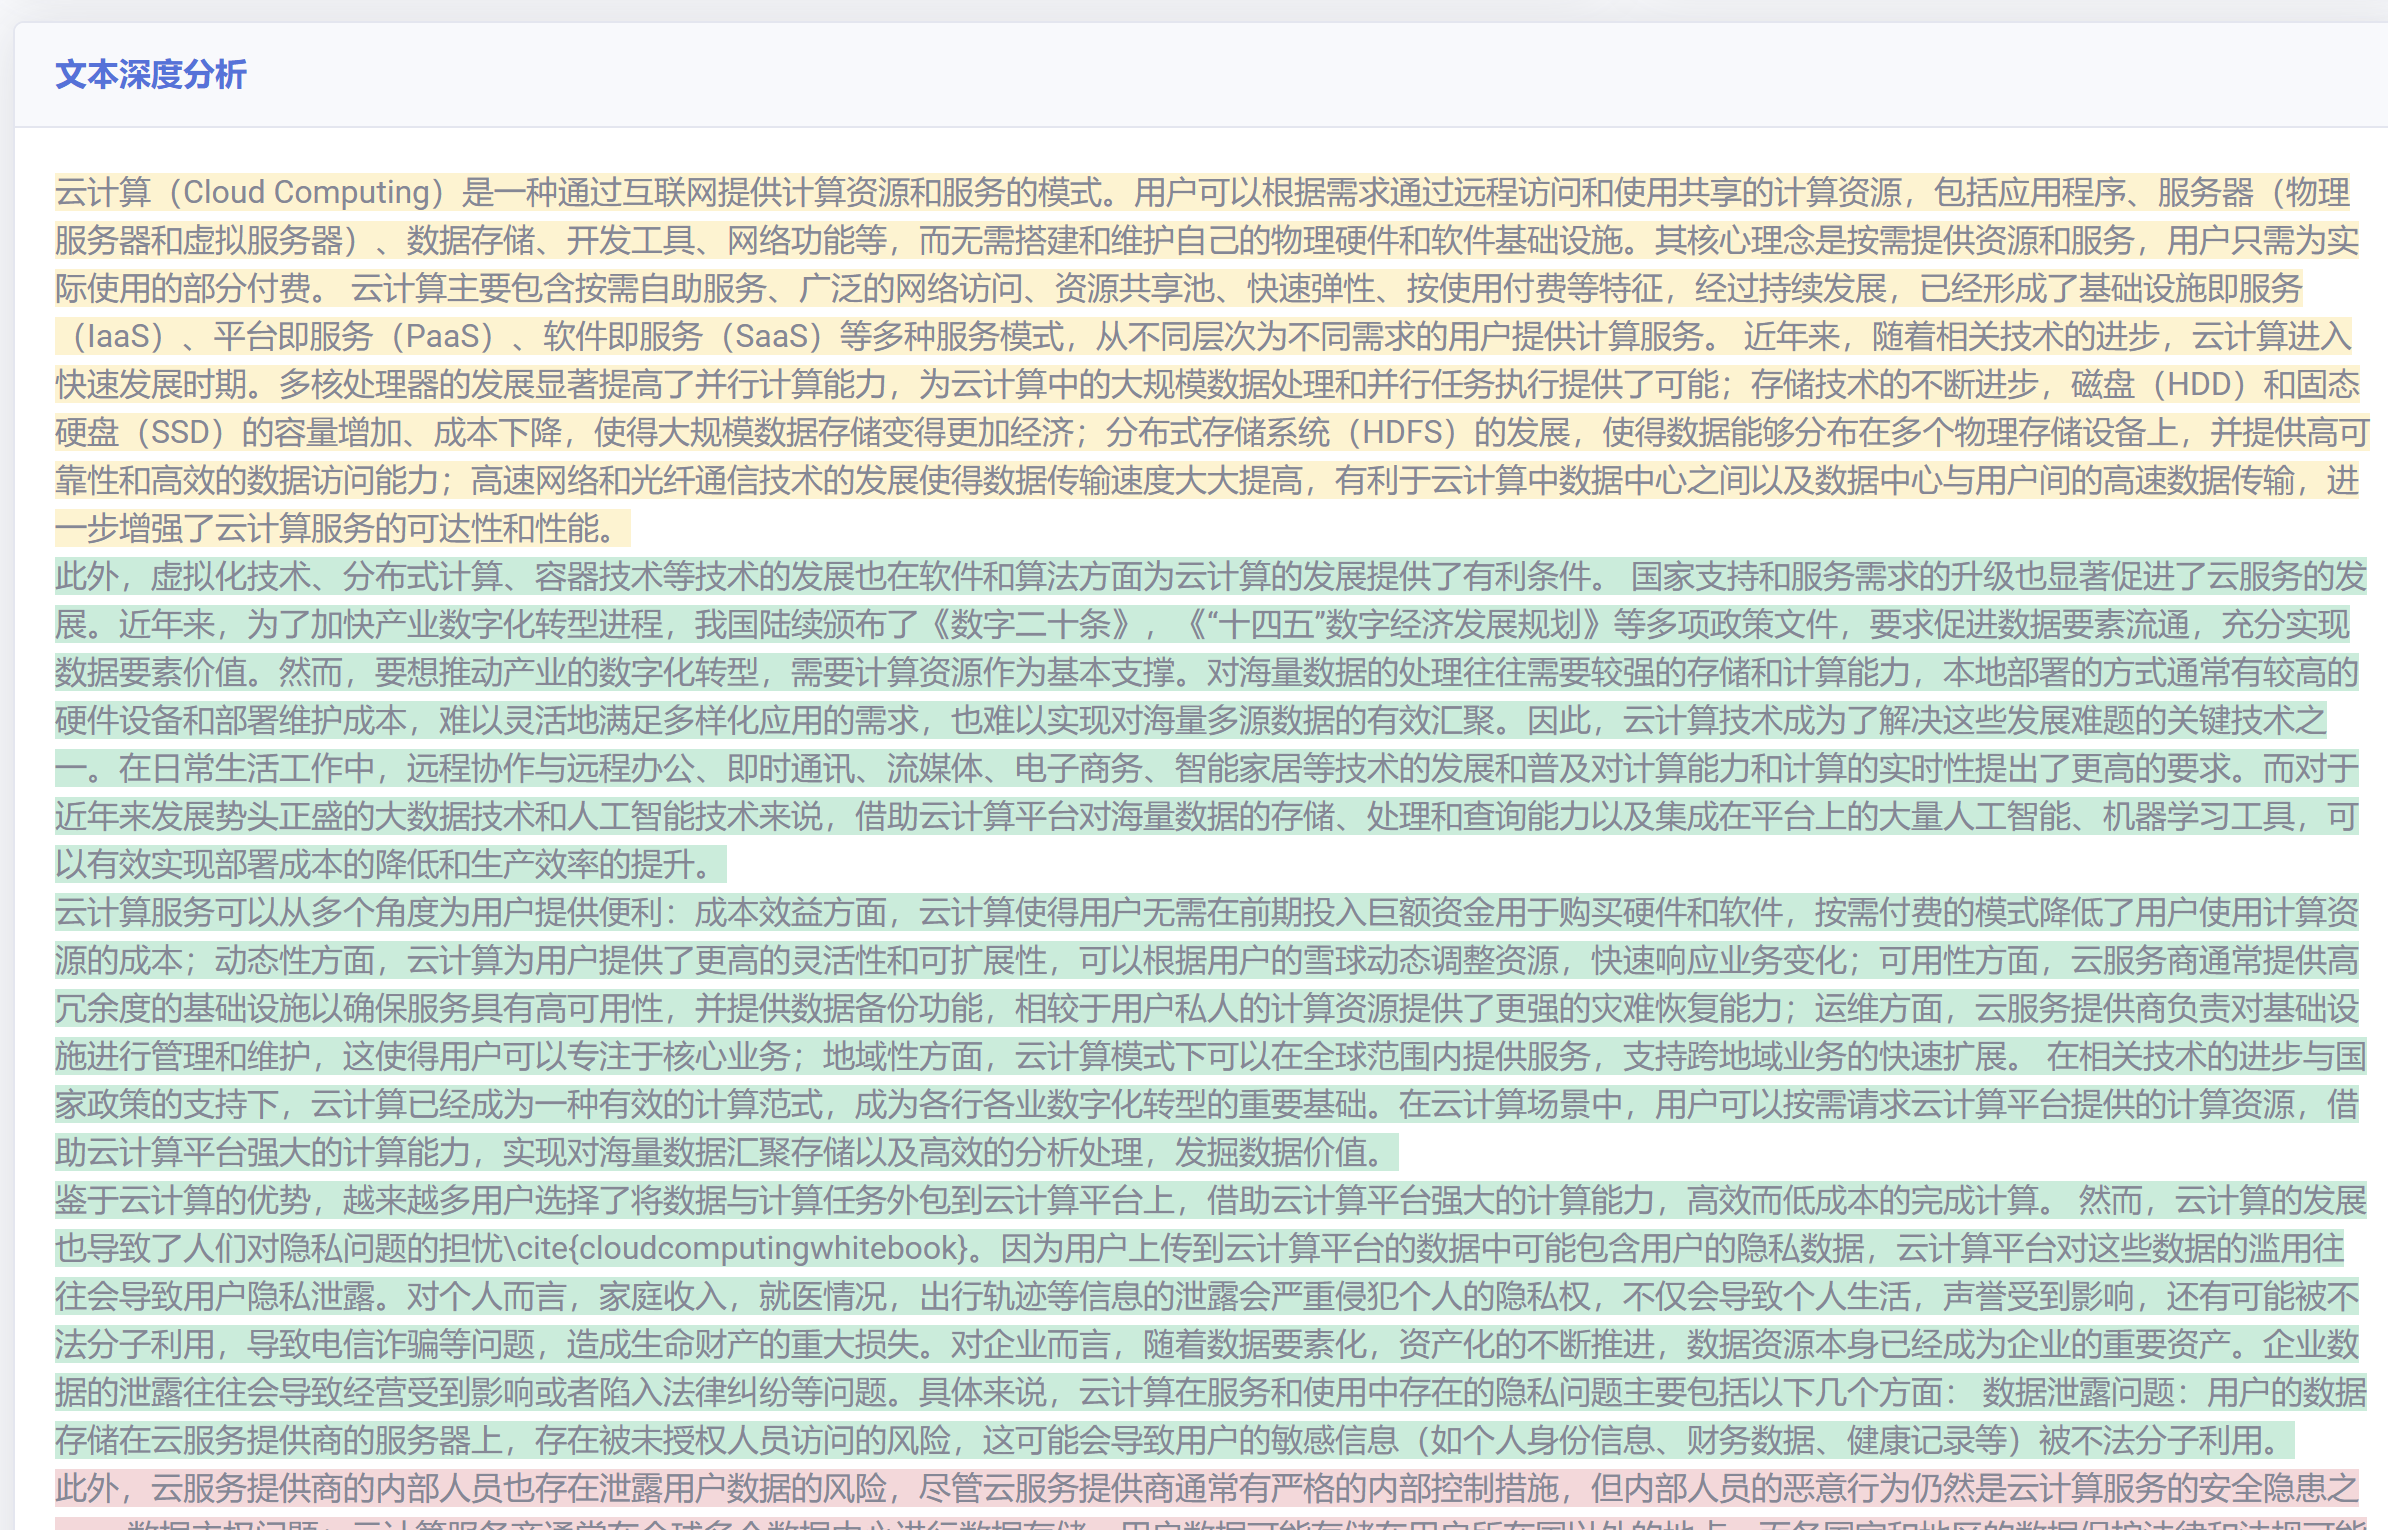
\includegraphics[width=\textwidth]{figures/文本深度分析.png}
	\caption{文本深度分析}
	\label{文本深度分析}
\end{figure}
如图\ref{文本深度分析}所示,红色部分高度疑似机器生成,黄色部分中度疑似机器生成,绿色部分为大概率人类生成。
\subsubsection{文件检测}%
如今的学术论文大多数文件格式为PDF格式,同时DOCX文件也要转换为PDF文件,TXT文件检测功能只是文本检测功能的锦上添花,所以这里注重展示PDF文件以及图片文件如何进行检测,以及最终检测的效果。

首先我们点击右下角的按钮,上传PDF文件进行检测,需要注意上传文件前要先选择不同的语言功能。
\begin{figure}[H]
	\centering
	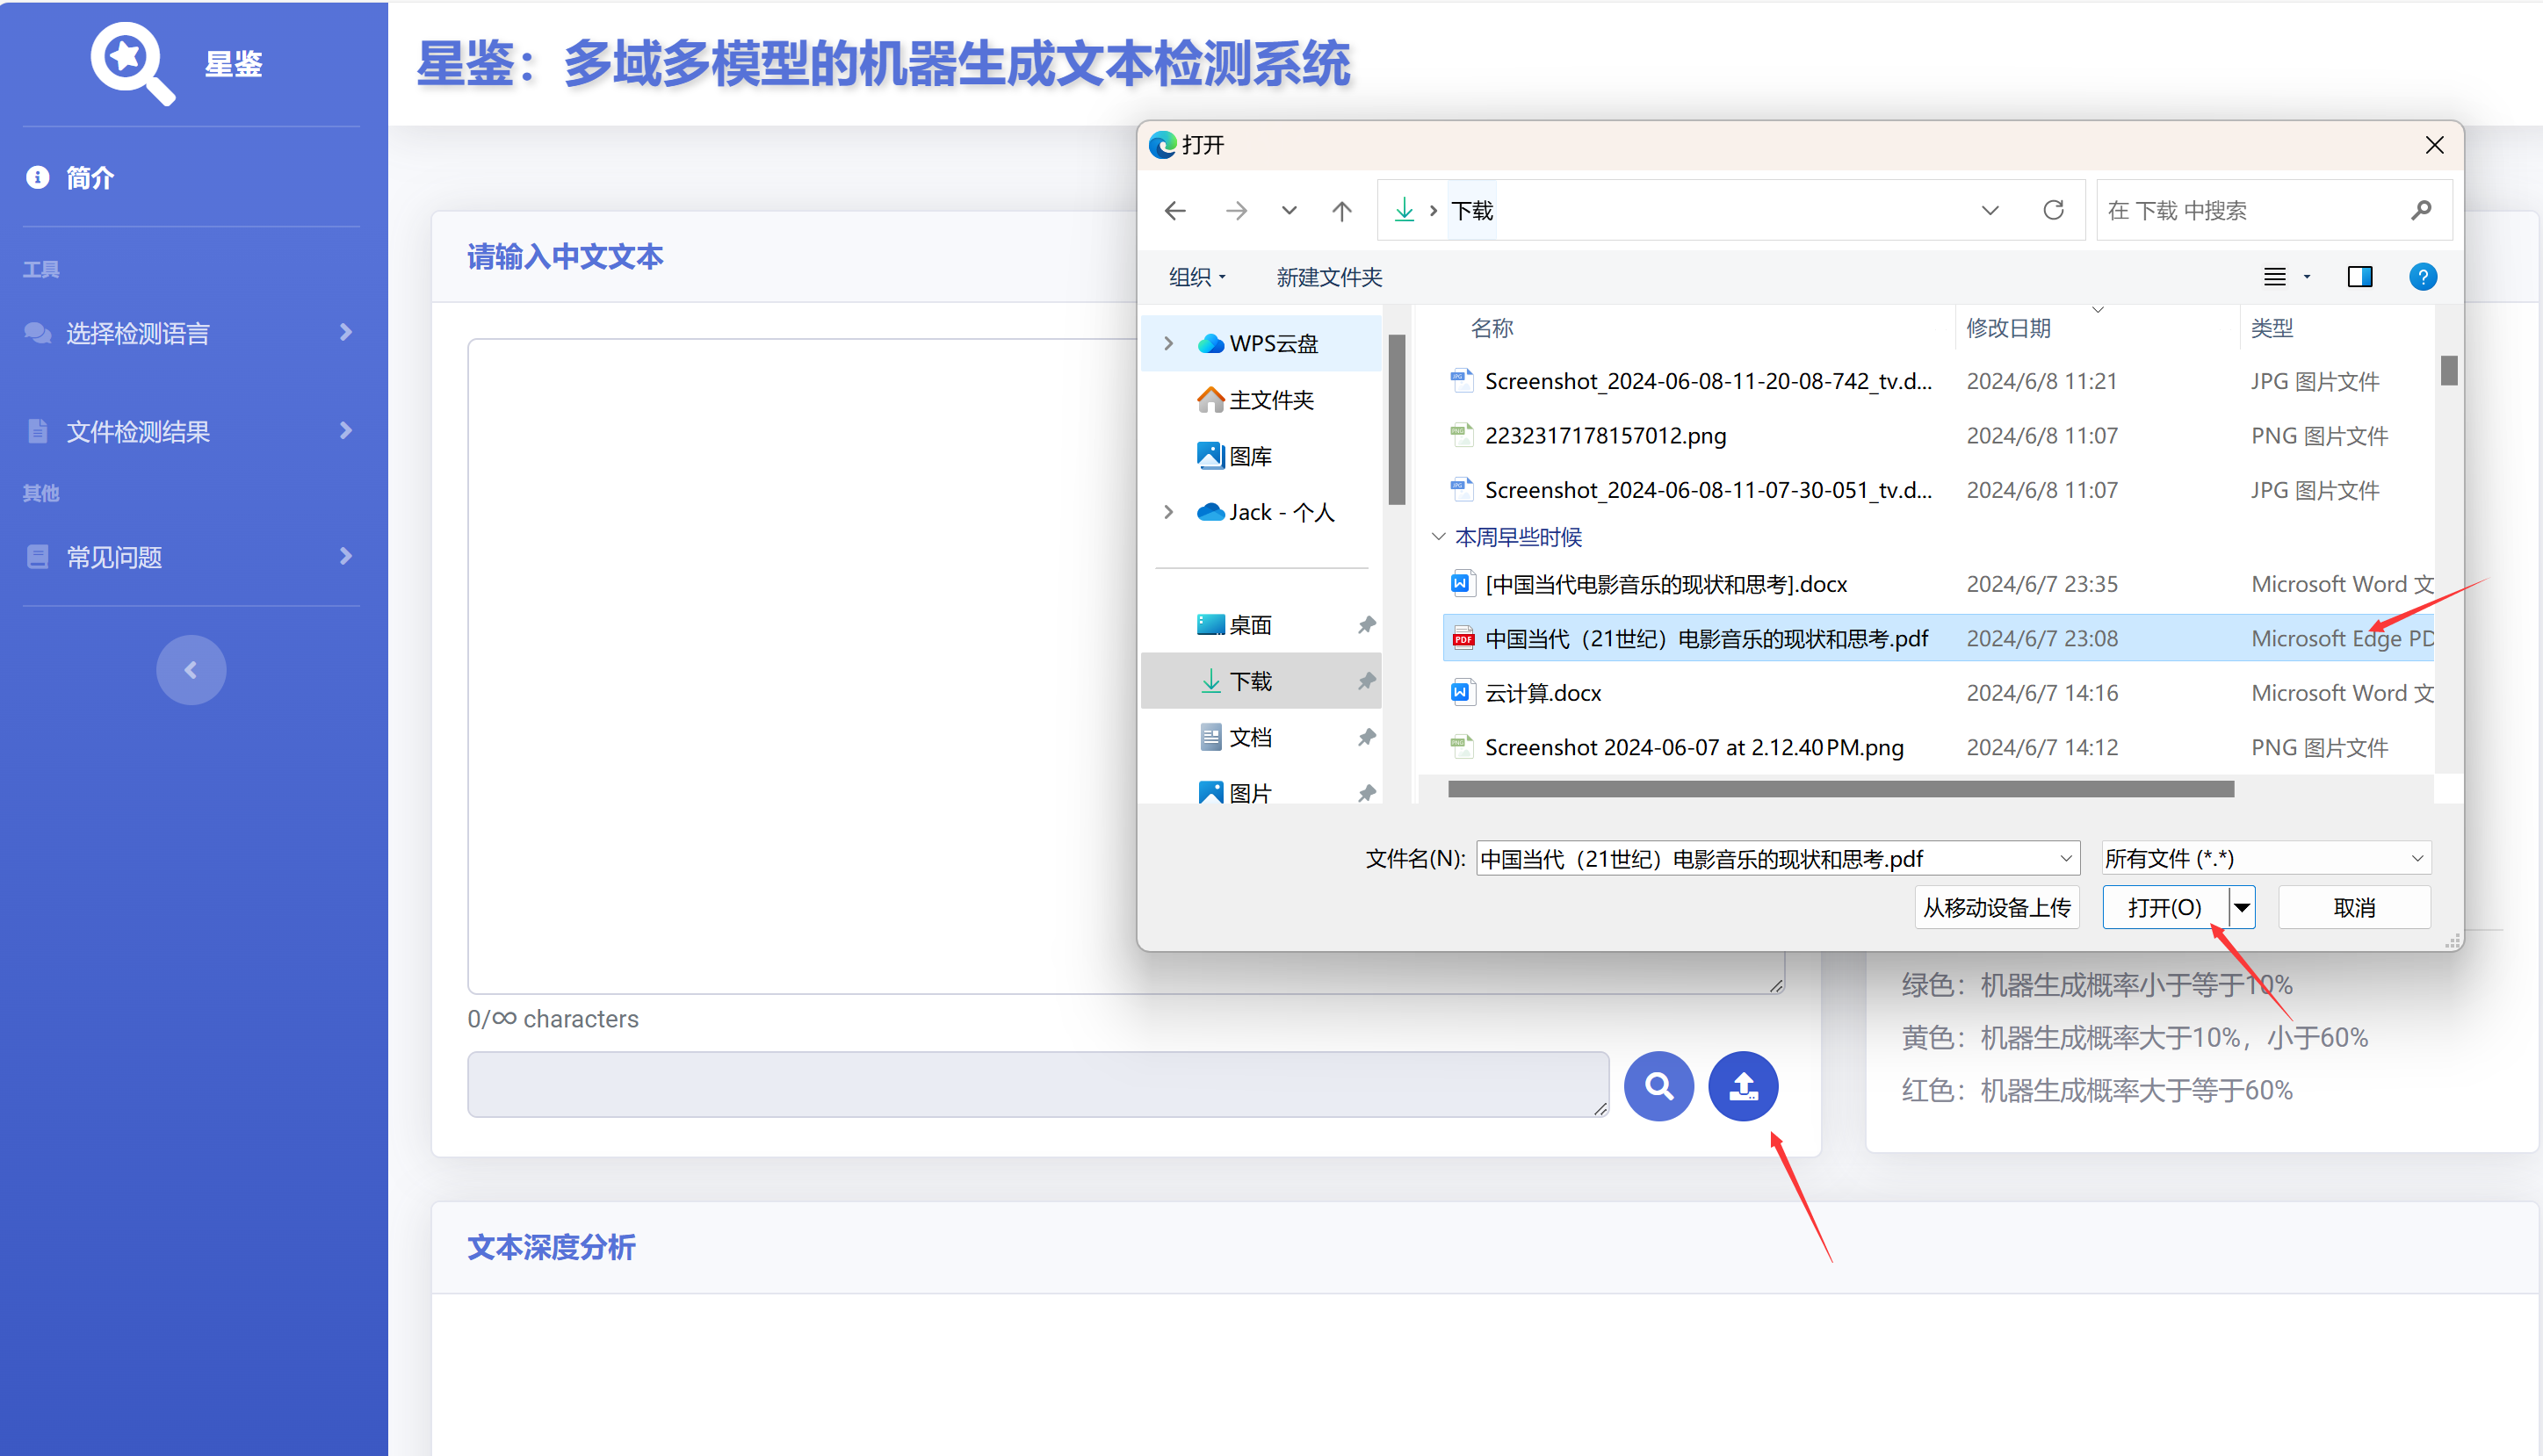
\includegraphics[width=\textwidth]{figures/上传文件检测.png}
	\caption{上传文件检测}
	\label{上传文件检测}
\end{figure}
检测完成之后,我们会在右边的文件检测结果中找到已经进行过标注的文件。
\begin{figure}[H]
	\centering
	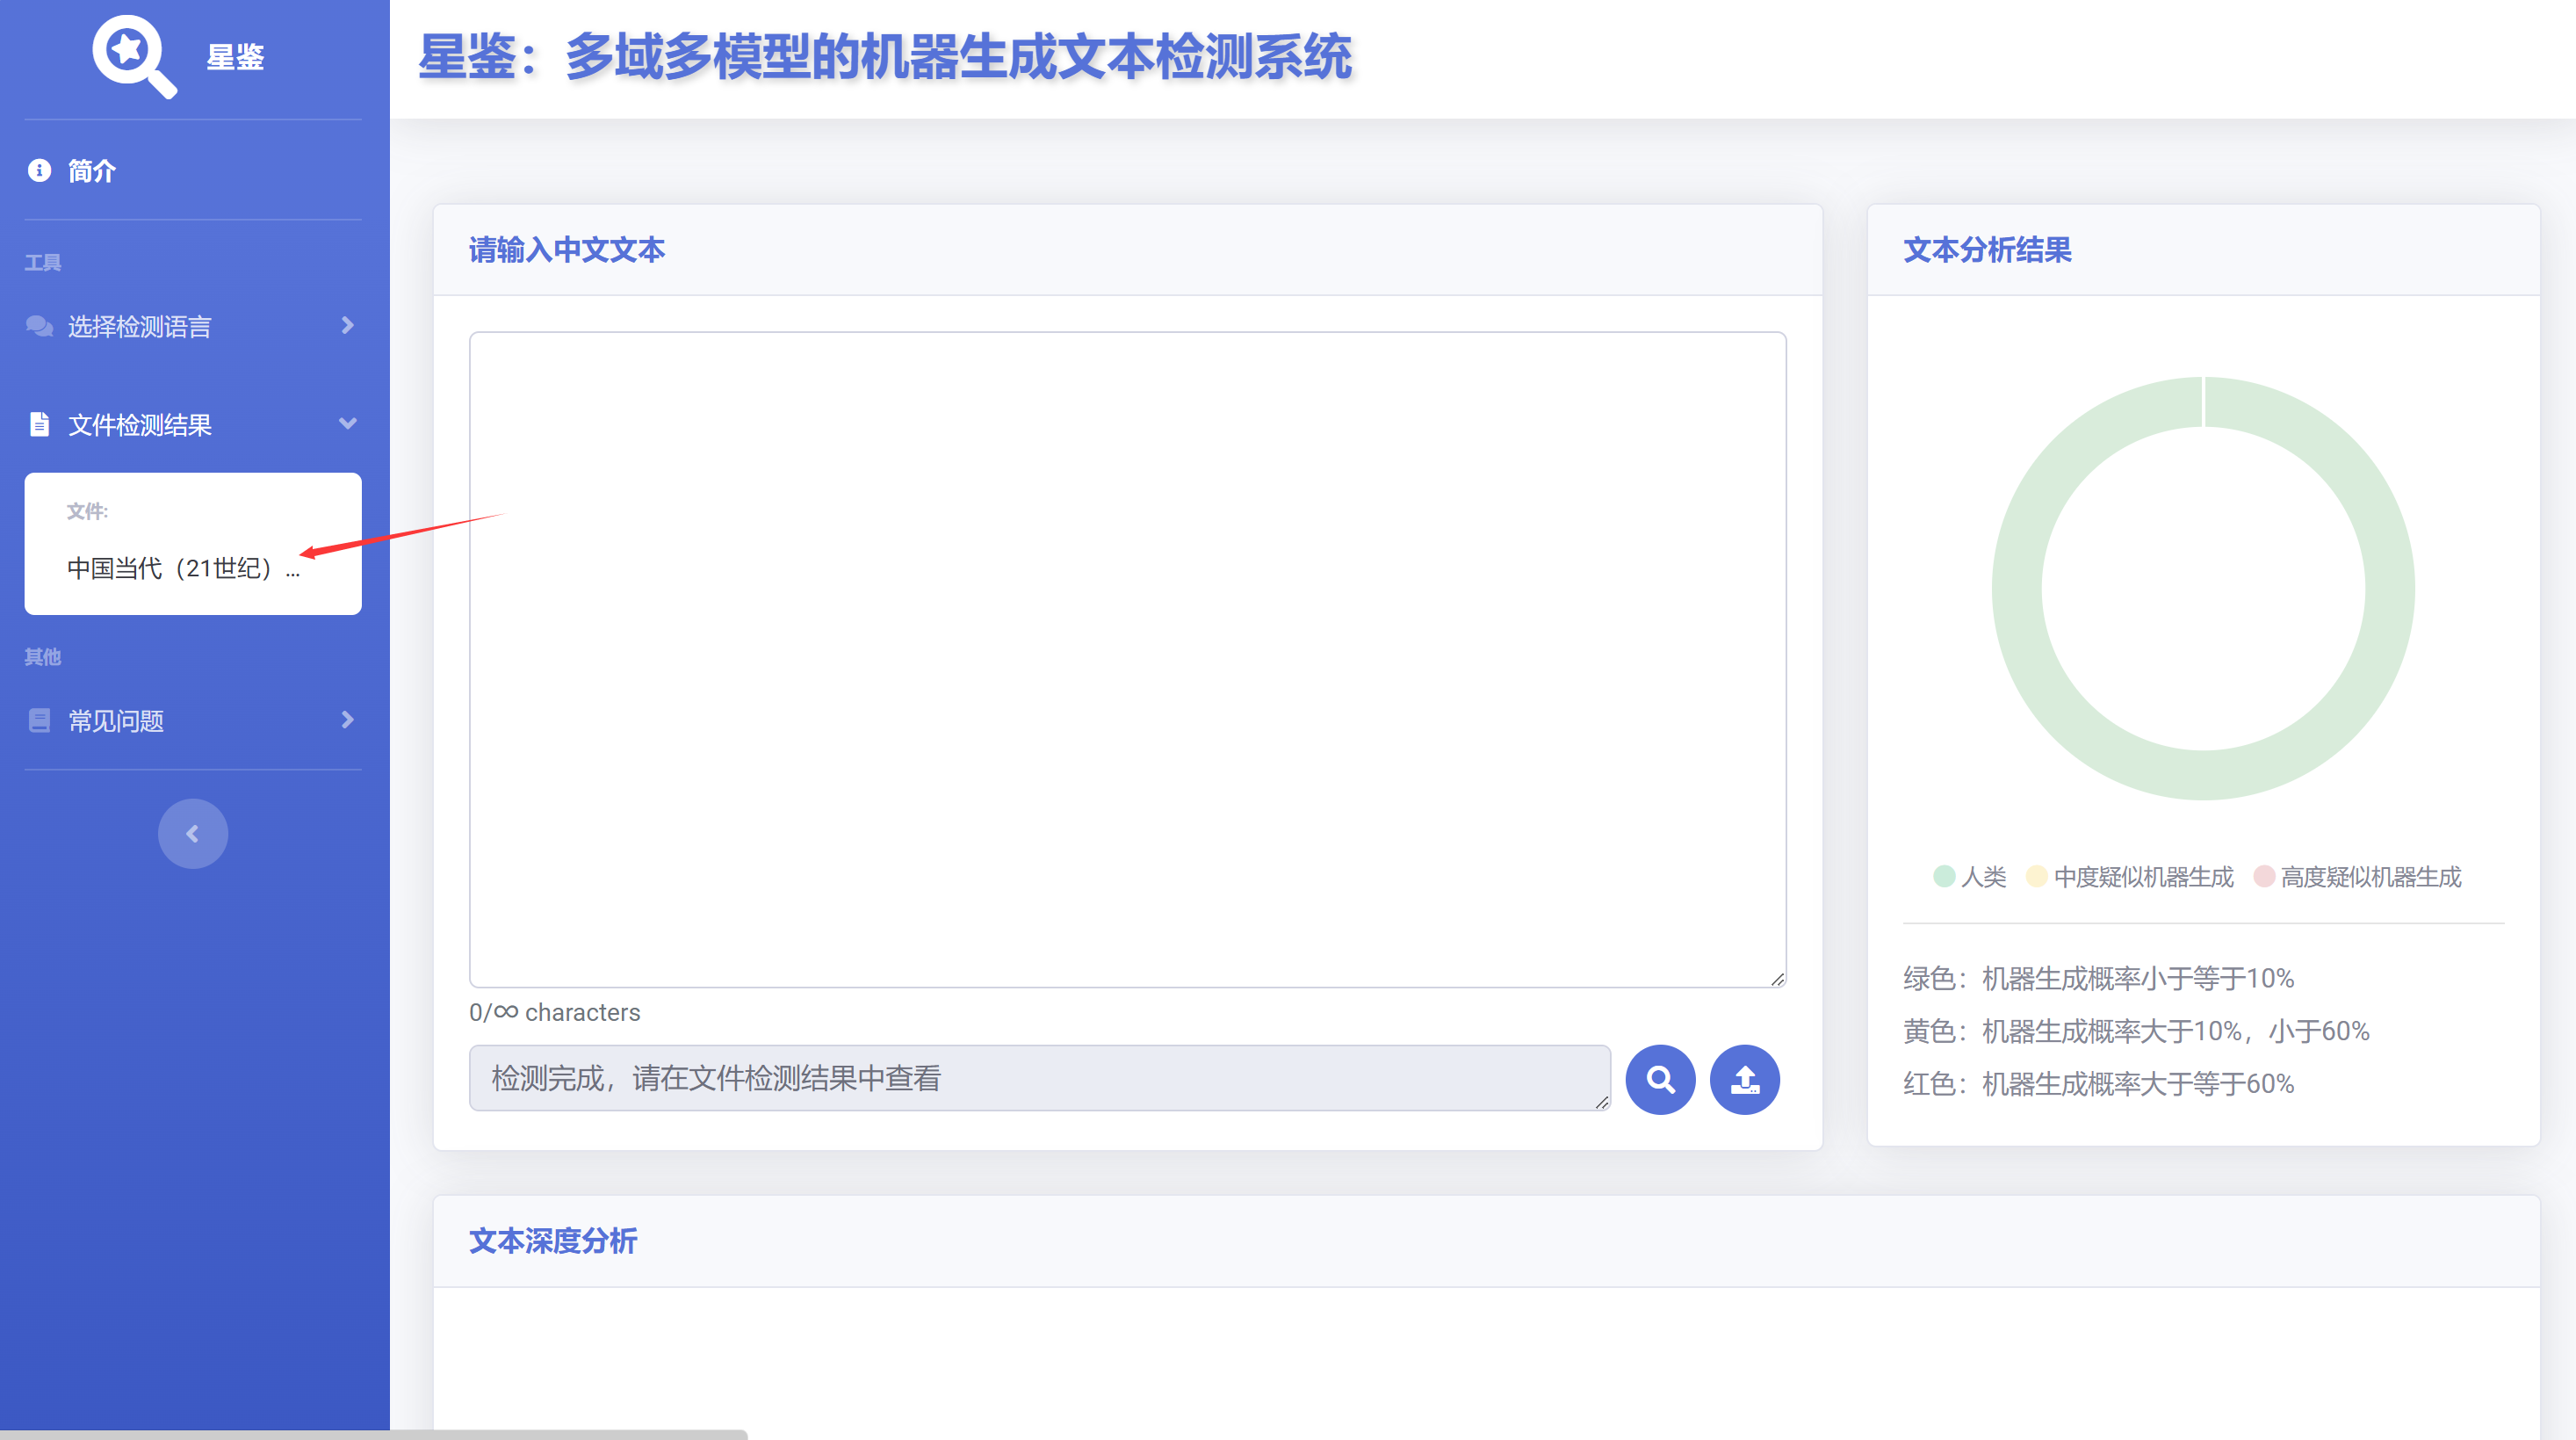
\includegraphics[width=\textwidth]{figures/文件检测结果.png}
	\caption{文件检测结果}
	\label{文件检测结果}
\end{figure}
我们点开文件检测结果,首先就可以看到一页检测报告,里面包含了检测时间,文件名,以及总体的机器生成概率评估和分布。
\begin{figure}[H]
	\centering
	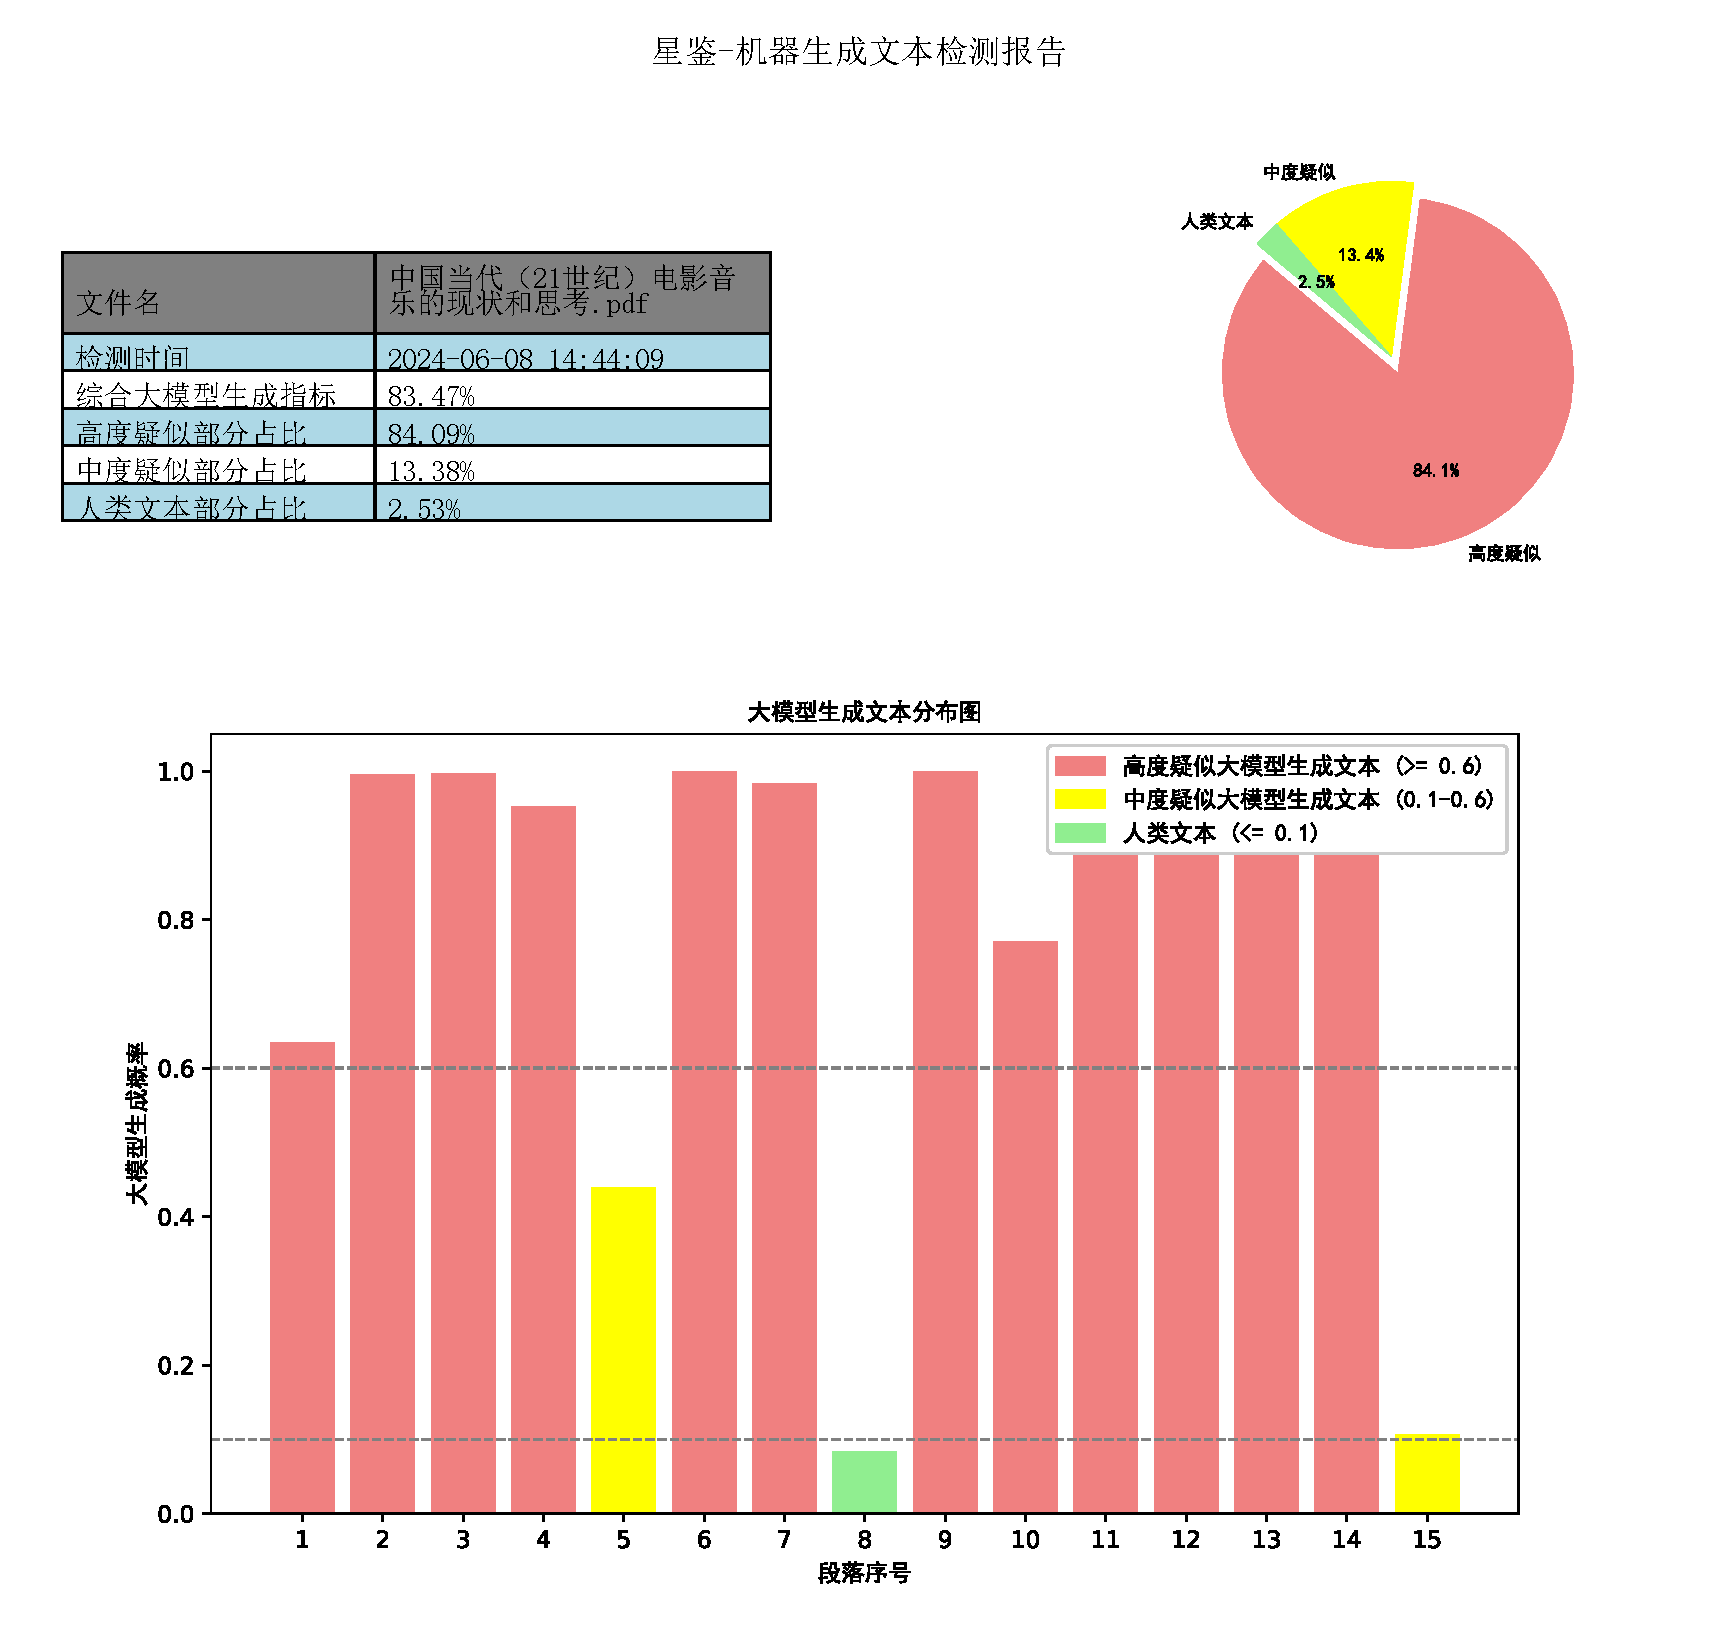
\includegraphics[width=0.83\textwidth]{figures/detection_report.pdf}
	\caption{星鉴---机器生成文本检测报告}
	\label{星鉴---机器生成文本检测报告}
\end{figure}

通过报告,我们可以看到整篇文章由机器生成的部分所占的比例,以及机器生成的文本部分在整个文章中的位置。

然后在每部分文本对应的位置右侧,都会有该部分是否由机器生成的标注以及生成的概率大小。
\begin{figure}[H]
	\centering
	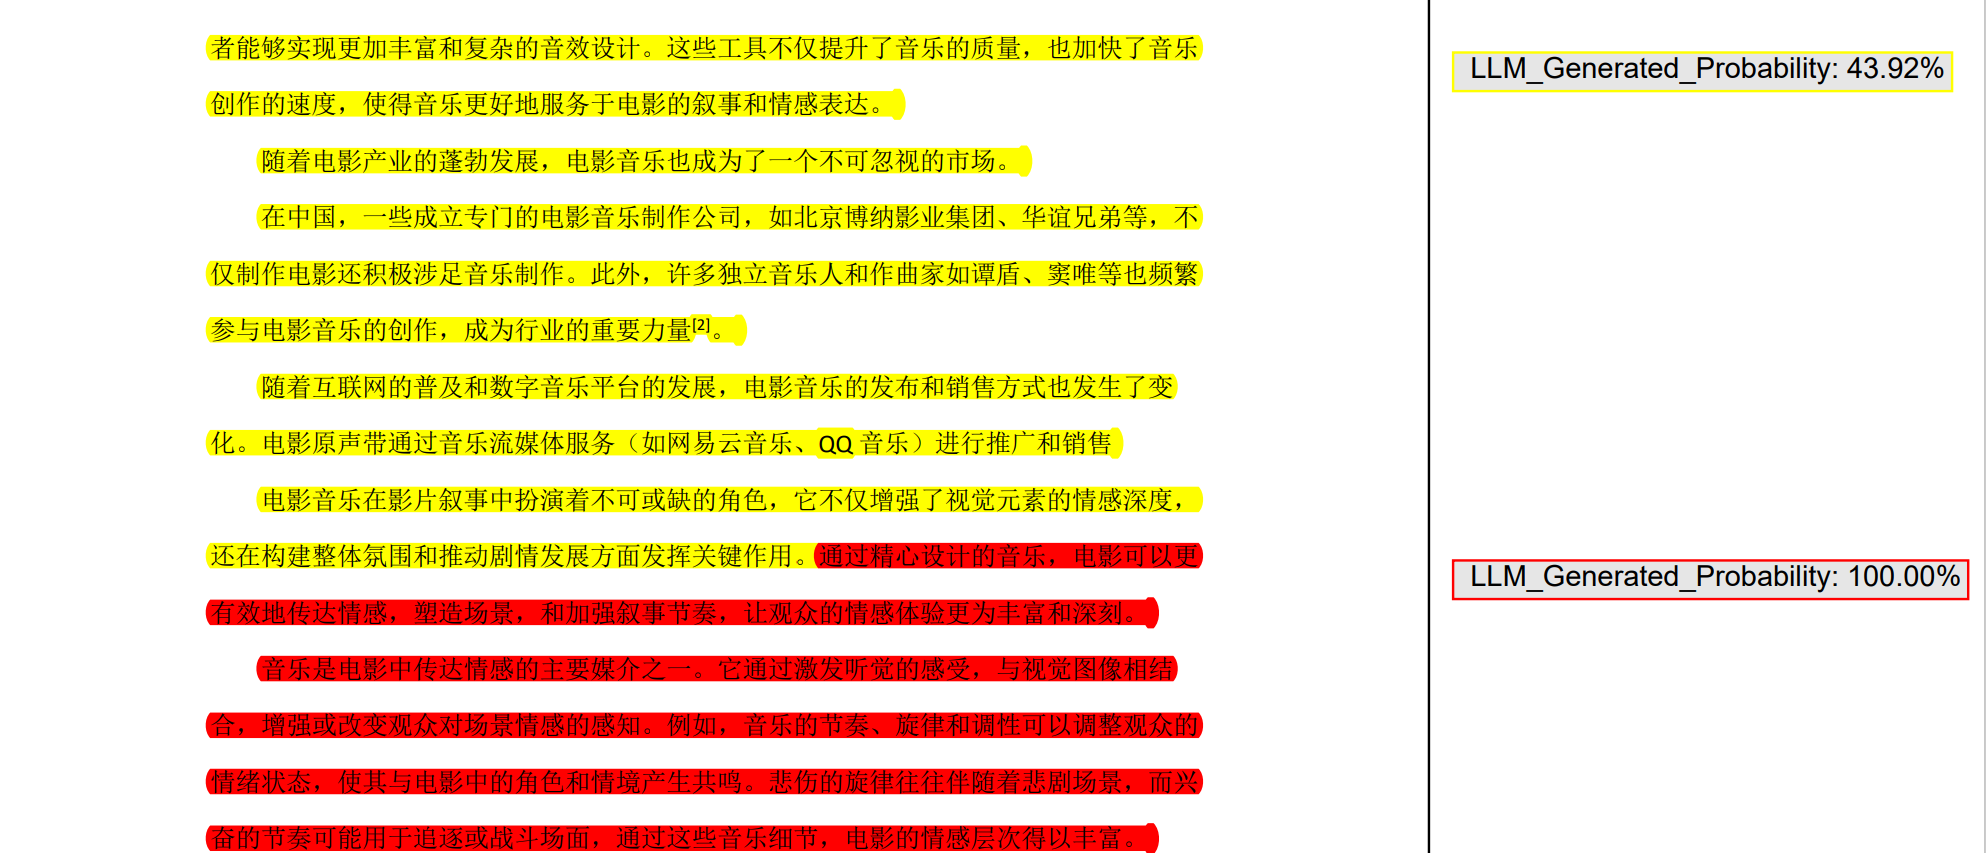
\includegraphics[width=\textwidth]{figures/PDF高亮结果.png}
	\caption{PDF文件标注}
	\label{PDF文件标注}
\end{figure}
同时我们也介绍一下提取图片文本进行检测的功能,首先我们先上传一张带有文字的图片
\begin{figure}[H]
	\centering
	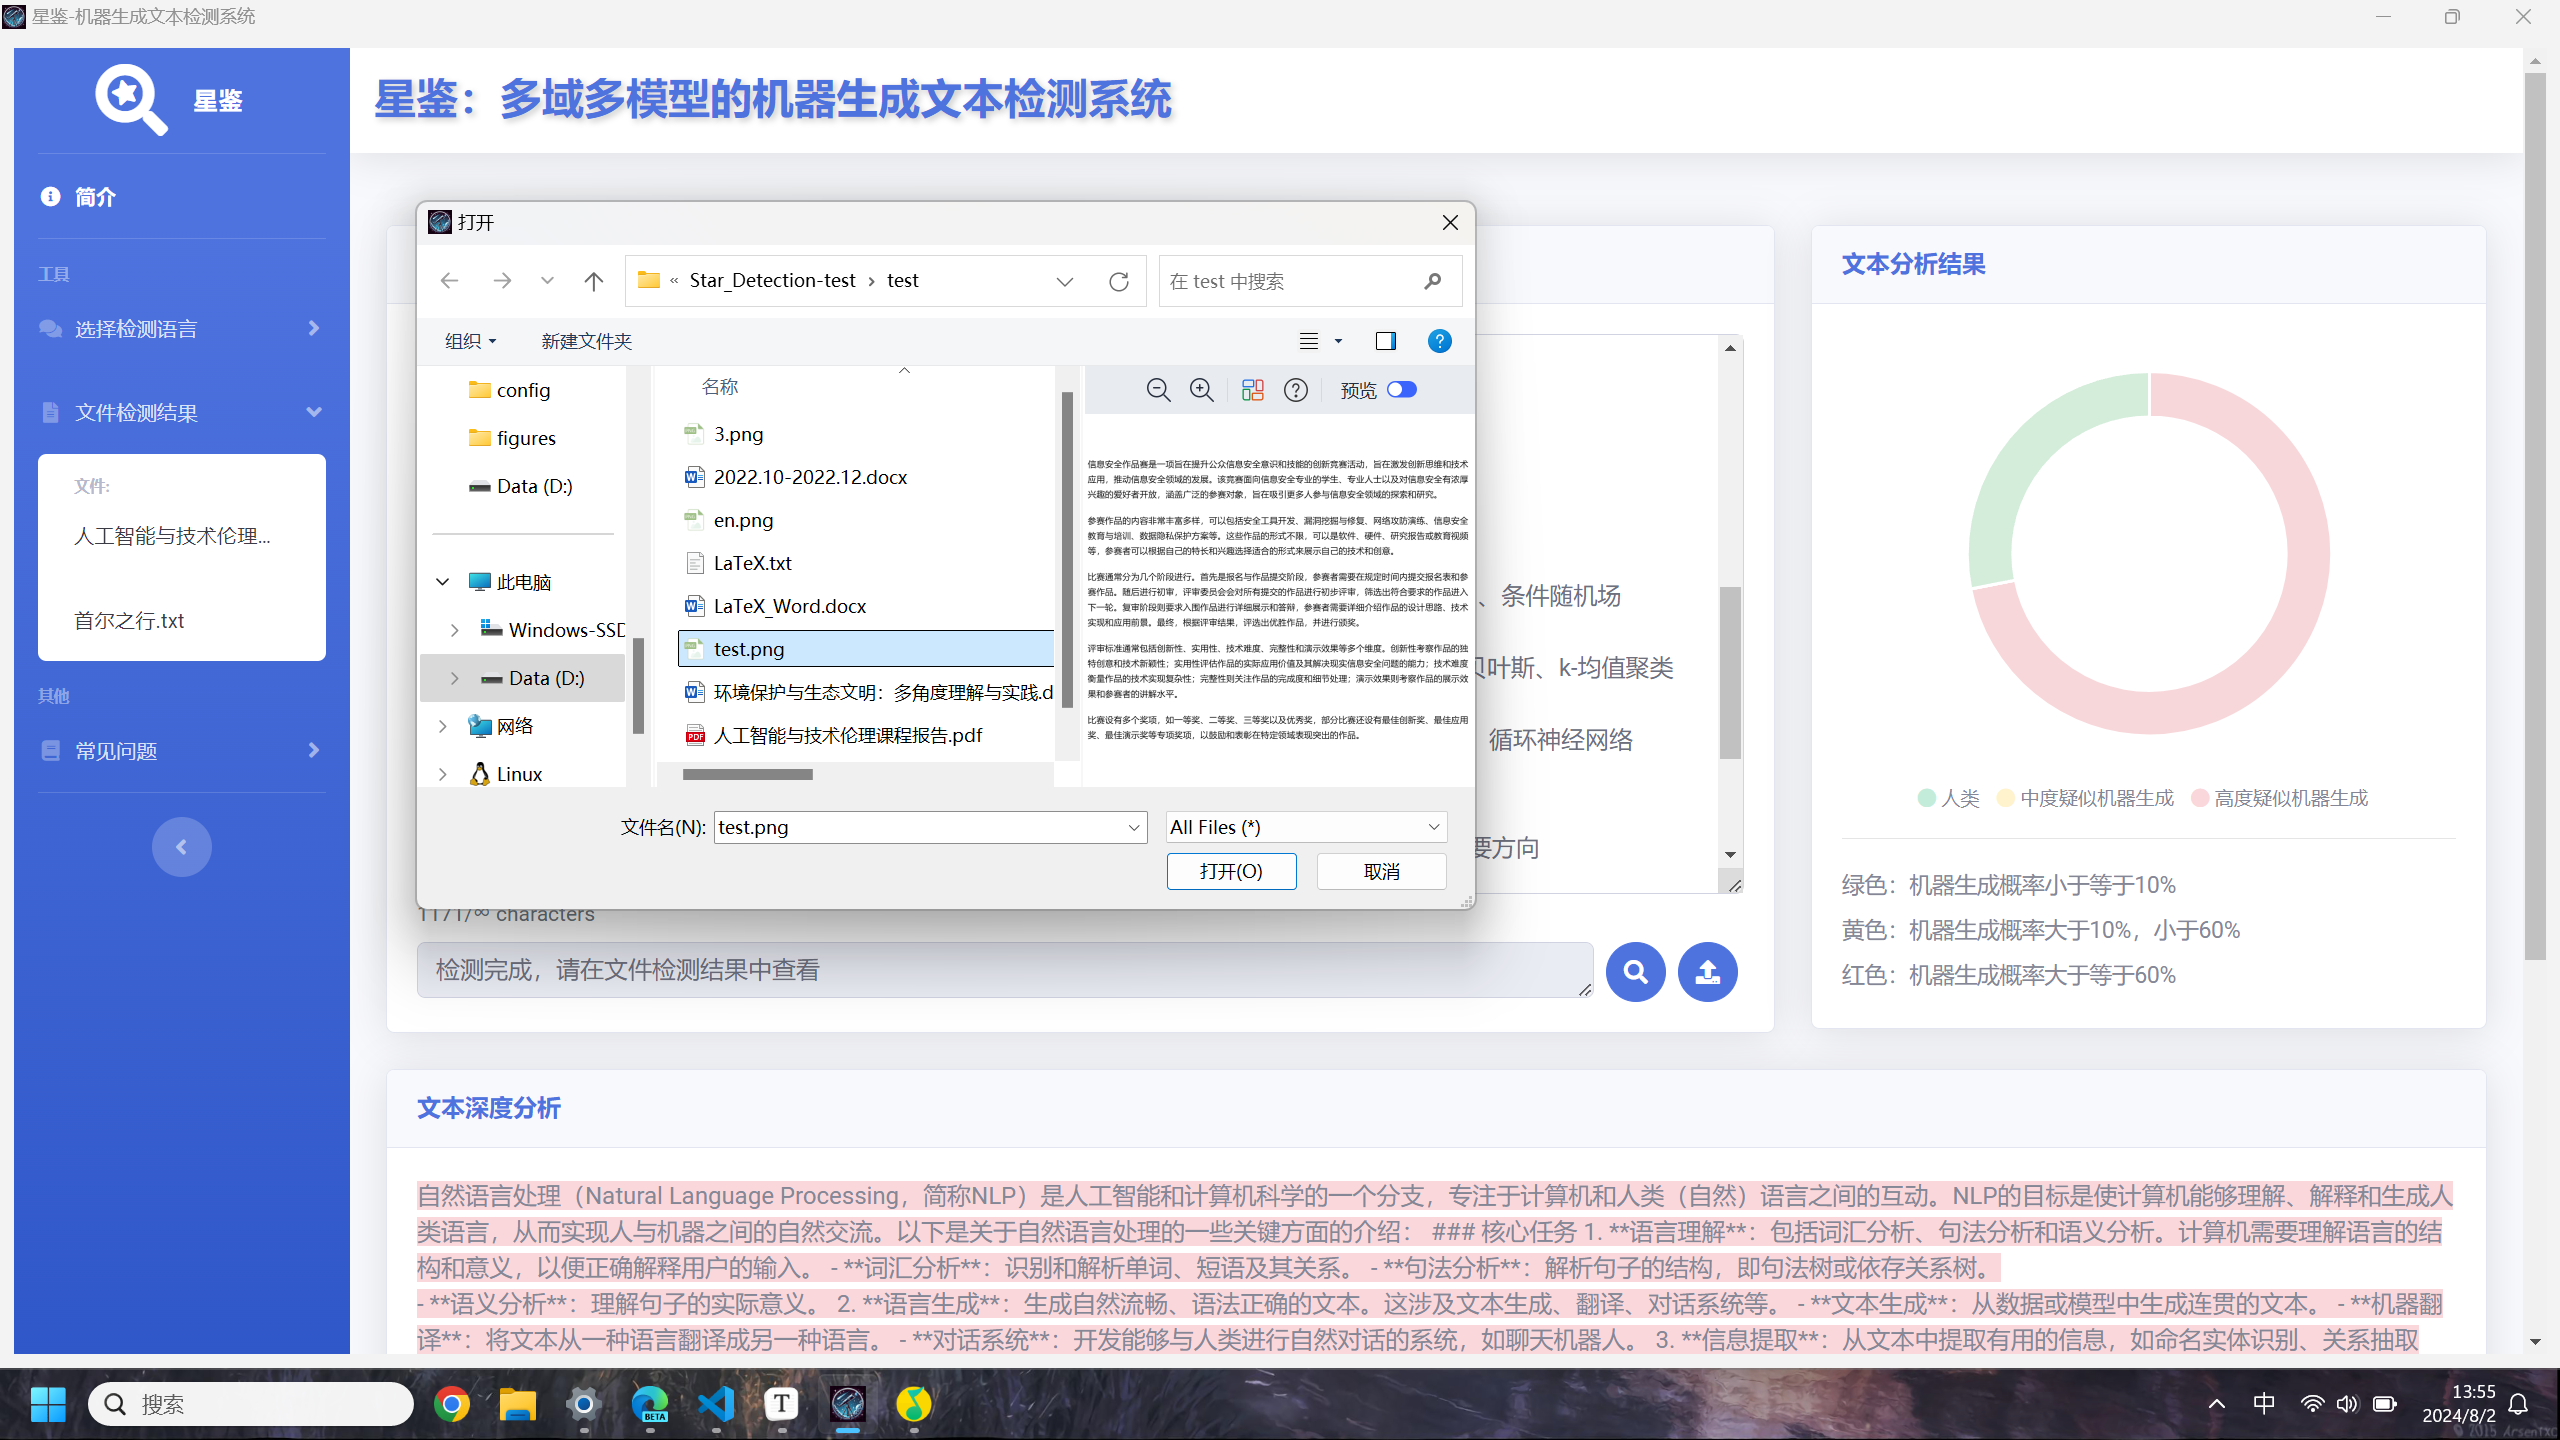
\includegraphics[width=\textwidth]{figures/upload_picture.png}
	\caption{上传图片检测}
\end{figure}
系统会先自动提取图片中的文字,例如这张图片中的文字就是:
\begin{example}
	信息安全作品赛是一项旨在提升公众信息安全意识和技能的创新竞赛活动,旨在激发创新思维和技术应用,推动信息安全领域的发展。该竞赛面向信息安全专业的学生、专业人士以及对信息安全有浓厚兴趣的爱好者开放,涵盖广泛的参赛对象,旨在吸引更多人参与信息安全领域的探索和研究。

	参赛作品的内容非常丰富多样,可以包括安全工具开发、漏洞挖掘与修复、网络攻防演练、信息安全教育与培训、数据隐私保护方案等。这些作品的形式不限,可以是软件、硬件、研究报告或教育视频等,参赛者可以根据自己的特长和兴趣选择适合的形式来展示自己的技术和创意。

	比赛通常分为几个阶段进行。首先是报名与作品提交阶段,参赛者需要在规定时间内提交报名表和参赛作品。随后进行初审,评审委员会会对所有提交的作品进行初步评审,筛选出符合要求的作品进入下一轮。复审阶段则要求入围作品进行详细展示和答辩,参赛者需要详细介绍作品的设计思路、技术实现和应用前景。最终,根据评审结果,评选出优胜作品,并进行颁奖。

	评审标准通常包括创新性、实用性、技术难度、完整性和演示效果等多个维度。创新性考察作品的独特创意和技术新颖性;实用性评估作品的实际应用价值及其解决现实信息安全问题的能力;技术难度衡量作品的技术实现复杂性;完整性则关注作品的完成度和细节处理;演示效果则考察作品的展示效果和参赛者的讲解水平。

	比赛设有多个奖项,如一等奖、二等奖、三等奖以及优秀奖,部分比赛还设有最佳创新奖、最佳应用奖、最佳演示奖等专项奖项,以鼓励和表彰在特定领域表现突出的作品。
\end{example}
经过OCR识别之后,图片中的文本会直接输入到文本检测的文本框中,由于识别不可能完全准确,所以可以允许用户自行修改编辑后再进行检测.
\begin{figure}[H]
	\centering
	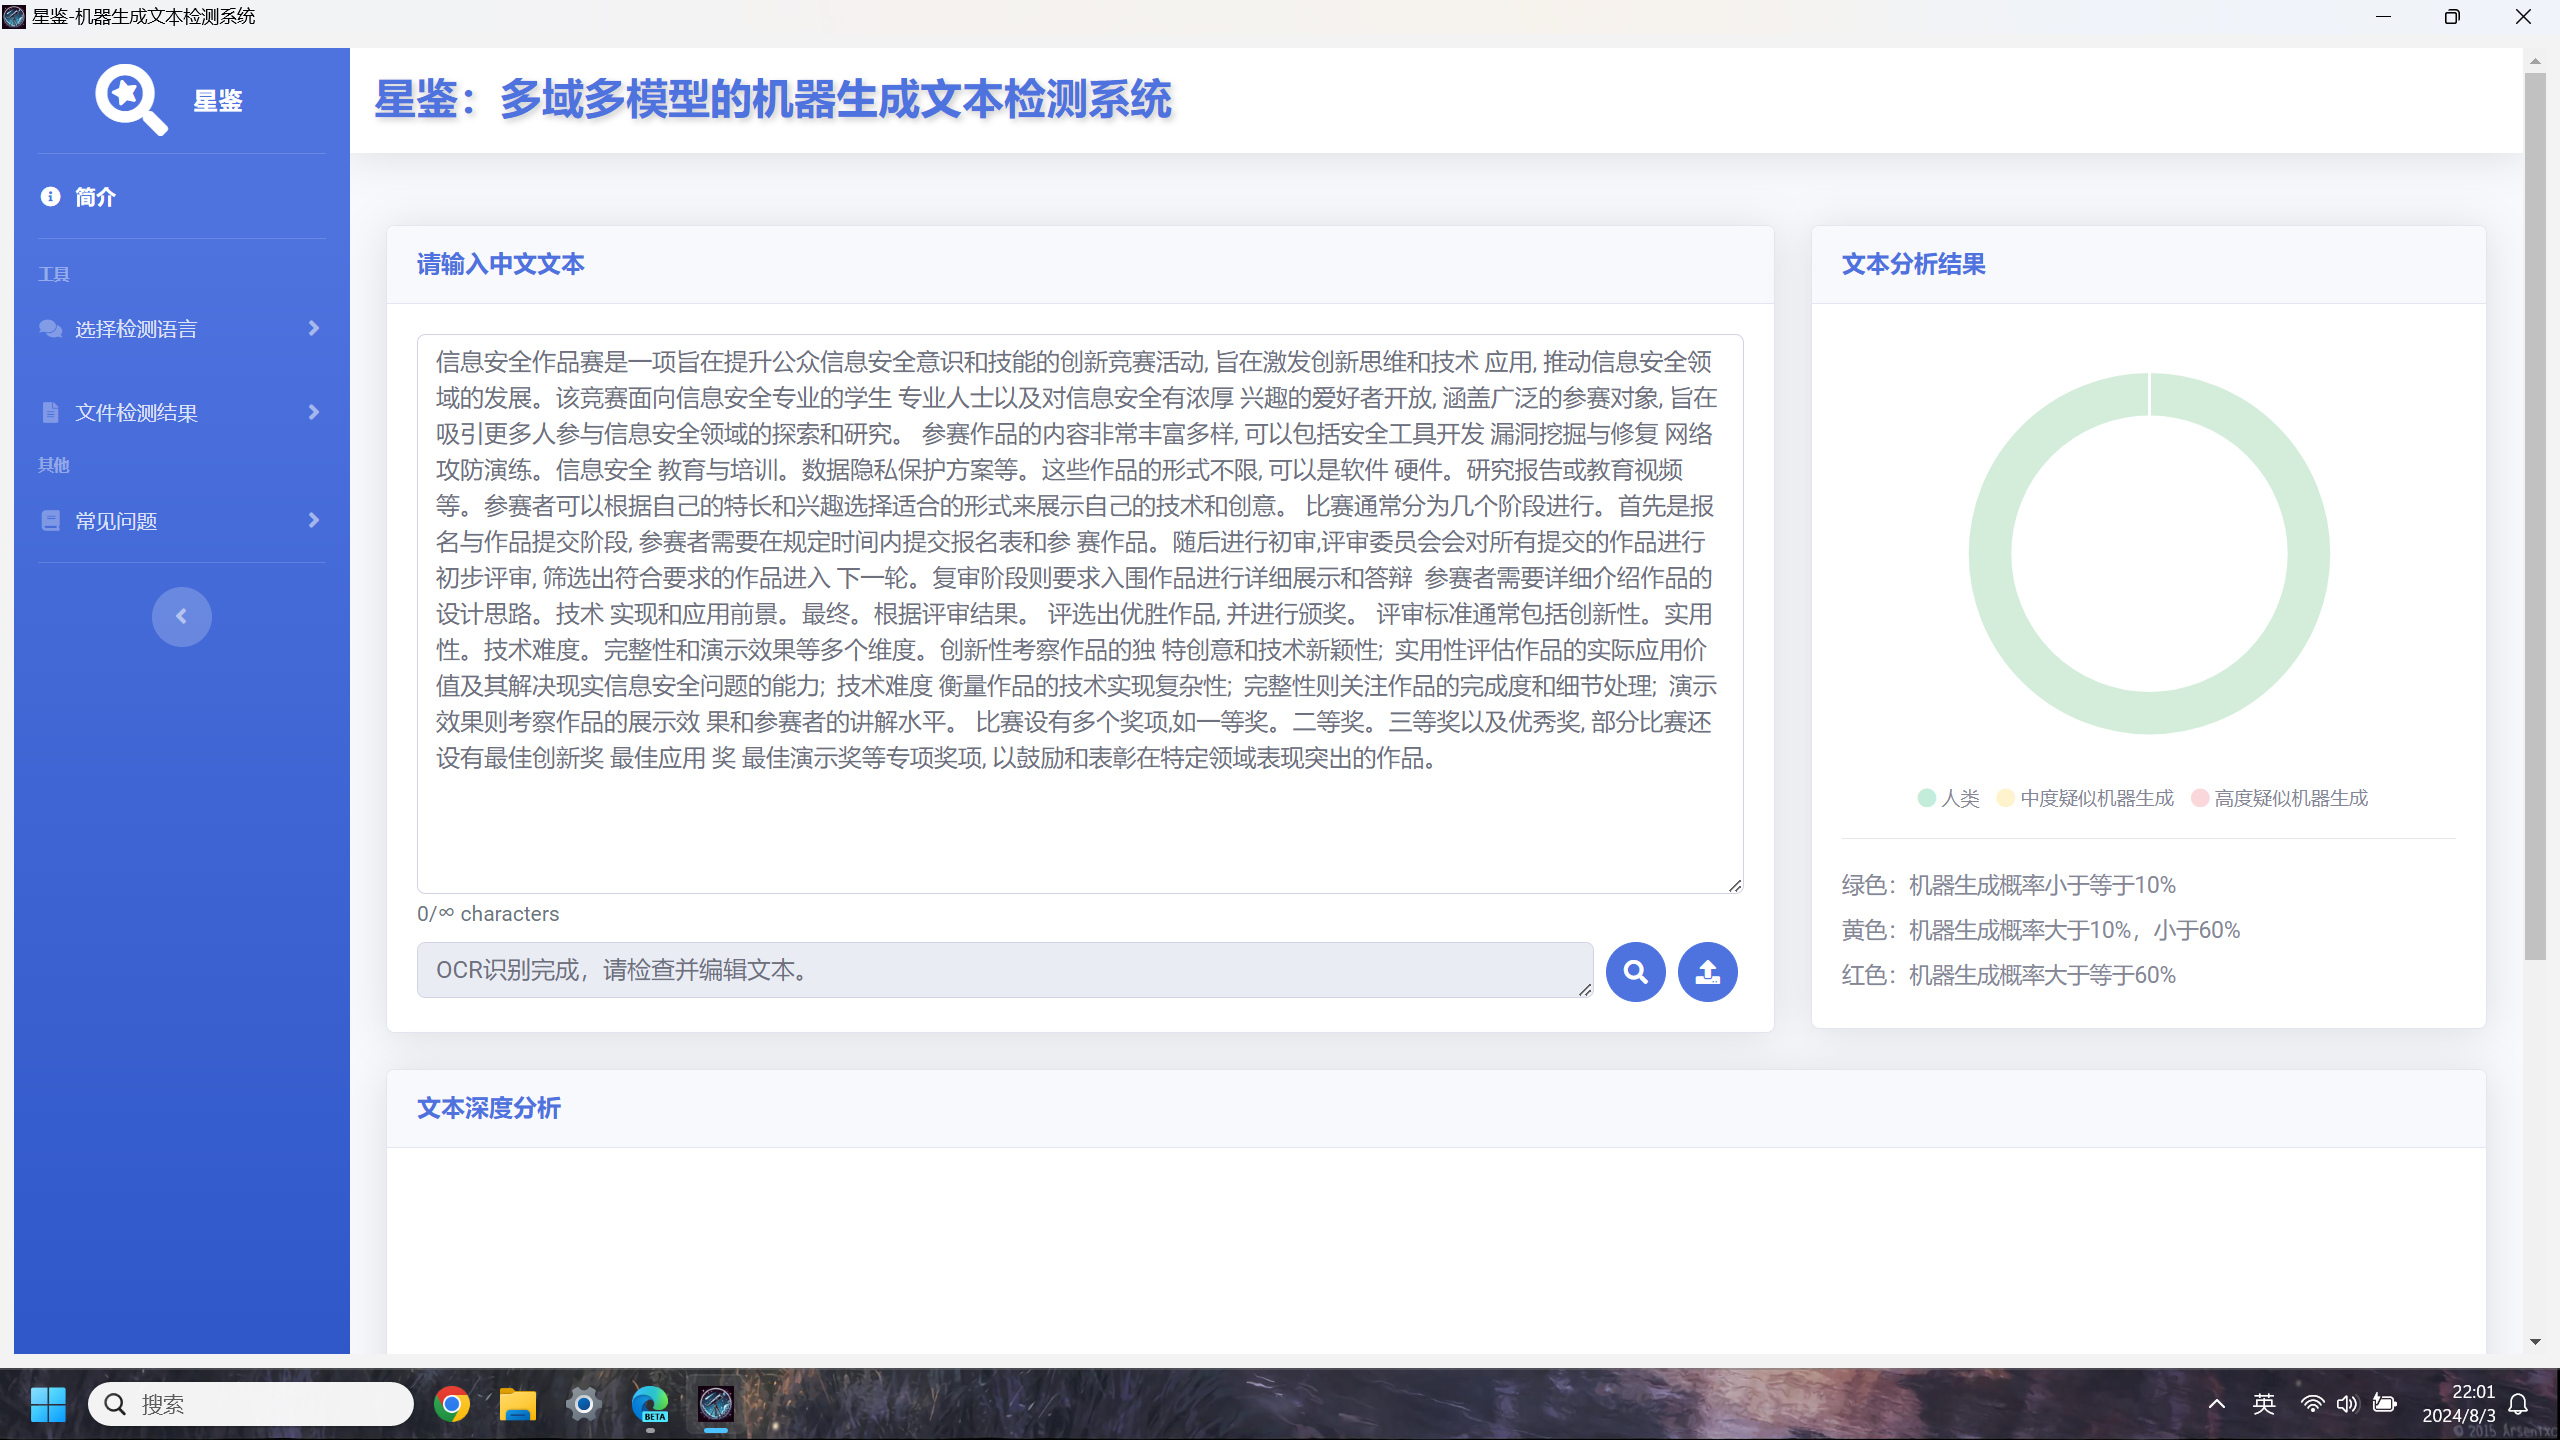
\includegraphics[width=\textwidth]{figures/OCR_result.png}
	\caption{图片识别结果}
\end{figure}
剩下的检测过程和检测结果和文本检测的部分完全相同。

\chapter{作品测试与分析}
%\section{测试方案}
\section{训练,测试及运行设备}
我们使用xlm-RoBERTa-base作为我们的预训练模型,在训练模型时,我们将batchsize设置为32,并采用Adamw优化器,初始学习率为5e−5。我们使用“瀚海”数据集训练模型。训练、验证和测试集的拆分比例为8:1:1。该模型在训练集上训练了10轮,同时加入早停机制,如果三轮内性能不再改善,则停止训练,最终根据其在验证集上的表现选择最佳模型。所有实验都在一台配备2张NVIDIA Telsa A100的工作站上进行。
\begin{table}[H]
	\centering
	\begin{tabular}{>{\centering\arraybackslash}p{5cm} >{\centering\arraybackslash}p{8cm}}
		\toprule
		配置   & 具体信息                                     \\
		\midrule
		操作系统 & Ubuntu 22.04                             \\
		\midrule
		CPU  & Intel(R) Xeon(R) Gold 5120 CPU @ 2.20GHz \\
		\midrule
		GPU  & NVIDIA Tesla A100(80G)$\times$ 2         \\
		\midrule
		内存   & 128GB                                    \\
		\bottomrule
	\end{tabular}
	\caption{模型训练及测试设备参数和设备环境}
\end{table}
训练完成后,检测系统可以部署在个人电脑上,服务端部署系统设备配置如下:
\begin{table}[H]
	\centering
	\begin{tabular}{>{\centering\arraybackslash}p{5cm} >{\centering\arraybackslash}p{8cm}}
		\toprule
		参数   & 配置参数值                                        \\
		\midrule
		操作系统 & Windows11                                    \\
		\midrule
		CPU  & AMD Ryzen 7 7840HS with Radeon 780M Graphics \\
		\midrule
		GPU  & 集成显卡                                         \\
		\midrule
		内存   & 32GB                                         \\
		\bottomrule
	\end{tabular}
	\caption{运行设备参数和设备环境}
\end{table}
\begin{table}[H]
	\centering
	\begin{tabular}{>{\centering\arraybackslash}p{5cm} >{\centering\arraybackslash}p{10cm}}
		\toprule
		参数    & 配置参数值               \\
		\midrule
		操作系统  & Ubuntu 20.04 64 位   \\
		\midrule
		CPU   & 16 核 (vCPU)         \\
		\midrule
		内存    & 60GiB               \\
		\midrule
		GPU   & NVIDIA A10*8(24GiB) \\
		\midrule
		公网 IP & 按量付费随时变化            \\
		\midrule
		公网带宽  & 100 Mbps (峰值)       \\
		\bottomrule
	\end{tabular}
	\caption{Web服务器配置信息}
\end{table}

\section{测试项目及测试数据}
\subsection{“星鉴”在域外的性能测试对比}
我们将“瀚海”数据集以及开源的英文数据集(包括HC3数据集,M4数据集等)随机挑选数据拆分成训练集,验证集,测试集,比例为$8:1:1$,并和Fast-DetectGPT,BERT,RoBERTa-Base在HC3数据集,M4数据集的中文部分以及Ghostbuster上比较性能,确保所有的数据对于星鉴都是域外数据。
\begin{figure}[H]
	\centering
	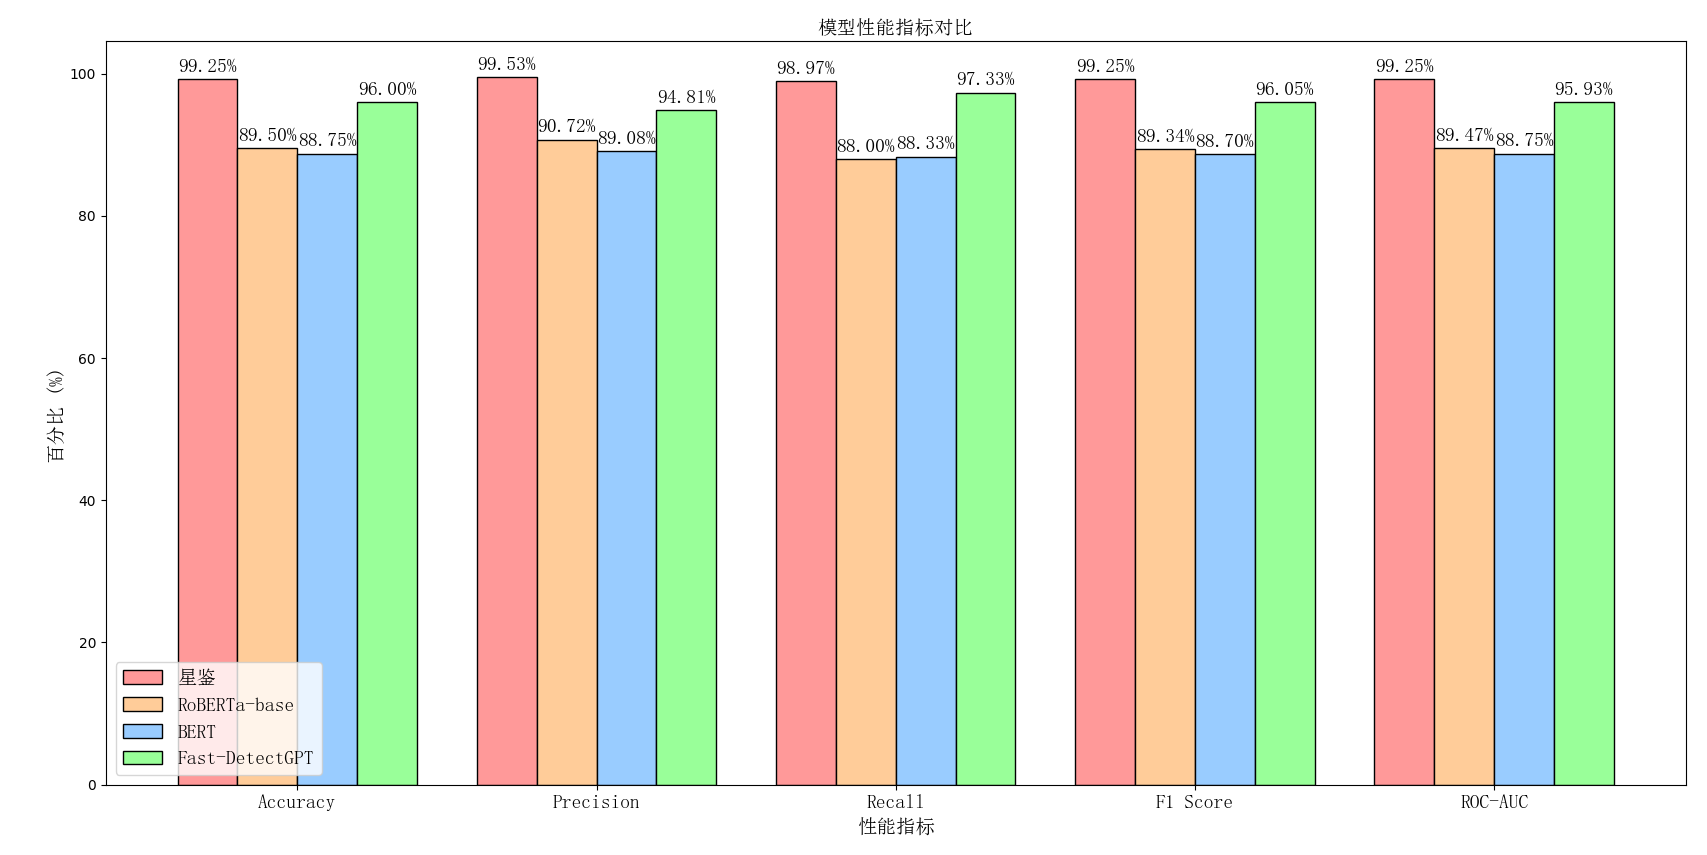
\includegraphics[width=\textwidth]{figures/星鉴和不同模型在域外数据的性能对比.png}
	\caption{星鉴和不同模型在域外数据的性能对比}
	\label{星鉴和不同模型在域外数据的性能对比}
\end{figure}
可以看到星鉴将监督学习和零样本检测的方法结合之后,彻底解决了传统监督学习泛化性差的问题,同时达到了极高的检测性能.
\subsection{“星鉴”在多模型数据上的性能测试}
我们测试了星鉴在多模型数据上的性能,如图所示
\begin{figure}[H]
	\centering
	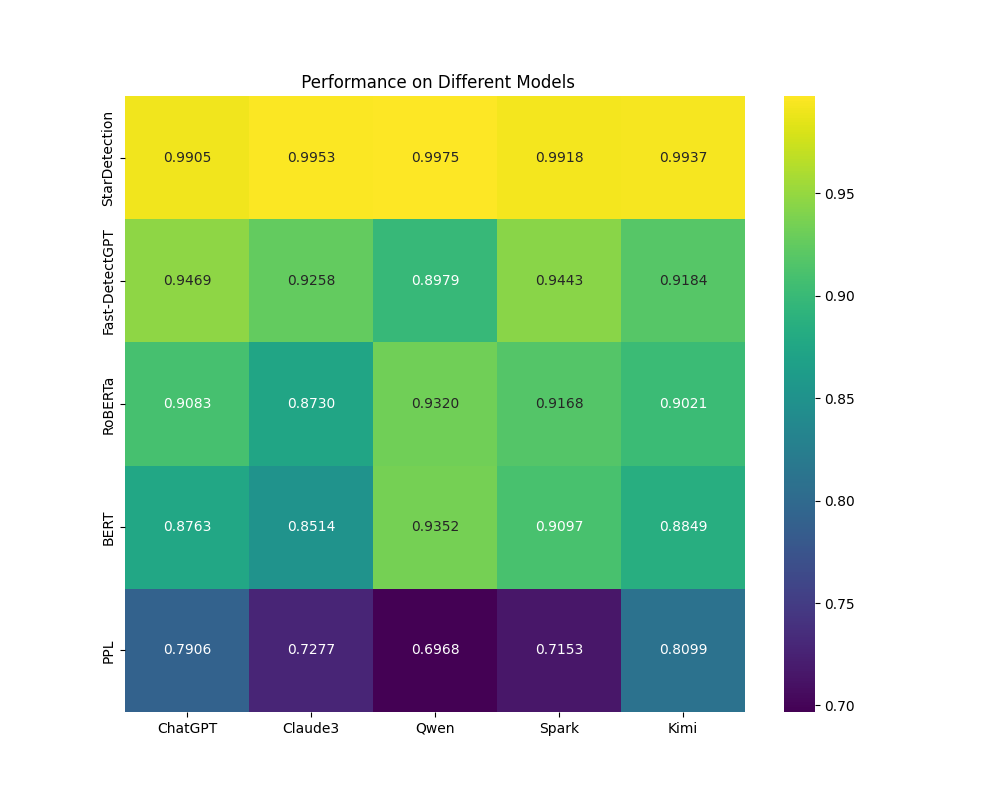
\includegraphics[width=\textwidth]{figures/不同模型性能对比.png}
	\caption{多模型数据性能对比图}
	\label{多模型数据性能对比}
\end{figure}
从图中可以看出星鉴在多模型数据上的都能达到99\%以上的准确率,全面领先目前的传统监督学习和零样本检测方法。
\subsection{检测速度对比}
我们控制变量,所有的计算过程都在一张Tesla A100(80G)GPU上运行,使用Fast-DetectGPT的数据集中的10000个样本,每个样本长度为150字。比较计算速度。
\subsubsection{“星鉴”零样本检测模块和Fast-DetectGPT速度对比}
我们比较了 Tesla A100 GPU 上 Fast-DetectGPT 和零样本检测模块的推理时间(不包括初始化模型的时间),Fast-DetectGPT需要2343秒(39分钟)可以完成任务,星鉴零样本检测模块只需要125秒可以完成任务,实现了约19倍的显著速度提升。

\begin{figure}[H]
	\centering
	\begin{tikzpicture}
		\begin{axis}[
				ybar,
				bar width=20pt, % Adjust the bar width as needed
				symbolic x coords={Fast-DetectGPT, 星鉴零样本检测模块},
				xtick=data,
				nodes near coords,
				ylabel={token/s},
				xlabel={模型},
				ymin=0, % Ensures bars start from 0
				ymax=15000,
				enlarge x limits=0.6, % Adjust x-axis limits
				axis y line*=left,
				axis x line*=bottom,
				width=15cm, % Increase width of the axis for a longer x-axis
				height=8cm, % Keep height the same
			]
			\addplot[fill=blue] coordinates {(Fast-DetectGPT, 640) (星鉴零样本检测模块, 12000)};
		\end{axis}

		% 加速因子文本
		\node at (4, 4) [red, above] {星鉴零样本检测模块实现约 $19 \times$ 的速度提升};
	\end{tikzpicture}
	\caption{任务完成时间对比}
\end{figure}




\subsubsection{“星鉴”和Fast-DetectGPT的检测速度对比}
我们使用完整的“星鉴”,再次比较了同任务下两者的检测速度。结合了监督学习模块之后,同样10000个样本的检测时间下降到22秒,相比较Fast-DetectGPT的2343秒,提升了107倍。
\begin{figure}[H]
	\centering
	\begin{tikzpicture}
		\begin{axis}[
				ybar,
				bar width=20pt, % Adjust the bar width as needed
				symbolic x coords={Fast-DetectGPT, 星鉴},
				xtick=data,
				nodes near coords,
				ylabel={Token/s},
				xlabel={模型},
				ymin=0, % Ensures bars start from 0
				ymax=70000,
				enlarge x limits=0.6, % Adjust x-axis limits
				axis y line*=left,
				axis x line*=bottom,
				width=15cm, % Increase width of the axis for a longer x-axis
				height=8cm, % Keep height the same
			]
			\addplot[fill=blue] coordinates {(Fast-DetectGPT, 640) (星鉴, 68181)};
		\end{axis}
		% 加速因子文本
		\node at (5, 4) [red, above] {结合监督学习模块,星鉴实现了约 $107 \times$ 的速度提升};
	\end{tikzpicture}
	\caption{任务完成时间对比}
\end{figure}




\subsection{不同长度文本的鲁棒性测试}

我们测试了各基准方法以及“星鉴”在不同长度文本上的准确性。



\begin{figure}[H]
	\centering
	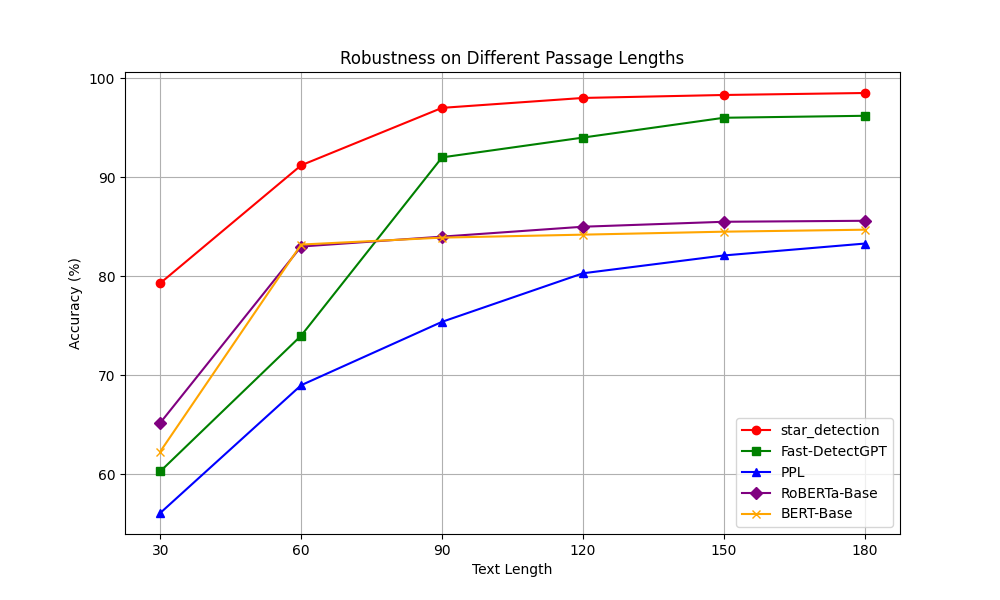
\includegraphics[width=\textwidth]{figures/Token.png}
	\caption{不同长度文本鲁棒性测试}
	\label{Token}
\end{figure}


可以发现,所有方法的准确性都会随着文本长度的增加而提高。“星鉴”对于文本长度并不敏感,在60个Token左右即可达到90\%以上的准确性.“星鉴”对于文本长度具有很强的鲁棒性。



\subsection{抗攻击测试}
我们选取最常用的释义攻击来进行抗攻击测试,释义攻击的定义已经在1.3.3进行了详细介绍,这里不再赘述。我们进行释义攻击,对测试集使用重写\cite{krishna2024paraphrasing},%需要引用那篇攻击论文
重写的参数配置为40L, 40O(表示词汇多样性为40\%,顺序多样性为40\%),然后分别在重写前后的测试集上进行测试,测试结果如下表所示:
\begin{table}[H]
	\centering
	\caption{攻击前后模型性能对比}
	\begin{tabular}{p{0.25\textwidth}p{0.15\textwidth}p{0.15\textwidth}p{0.2\textwidth}}
		\toprule
		准确率(Accuracy)  & 攻击前    & 攻击后    & 下降程度   \\
		\midrule
		星鉴             & 0.9926 & 0.9591 & 0.0335 \\
		Fast-DetectGPT & 0.9646 & 0.8598 & 0.1048 \\
		PPL(困惑度)       & 0.8080 & 0.6477 & 0.1603 \\
		RoBERTa        & 0.8663 & 0.7477 & 0.1186 \\
		BERT           & 0.8569 & 0.7113 & 0.1456 \\
		\bottomrule
	\end{tabular}
\end{table}

通过实验发现,“星鉴”在攻击前后的性能下降并不明显,抗攻击性显著优于其余监督学习方法以及零样本检测的方法。因此,“星鉴”能够很好的检测经过人工润色,人机混写的文本,具有很强的抗攻击能力以及良好的鲁棒性。


\subsection{“星鉴”和目前市面上的AIGC检测系统效果对比}
目前国内已经商用的AIGC检测系统主要是知网和维普,维普的AIGC检测系统介绍较为简洁:\textbf{维普AIGC检测:适用于AI生成的中文文本内容检测。}

知网的AIGC检测系统介绍比较复杂,总结如下:
\begin{table}[H]
	\centering
	\begin{tabular}{|>{\raggedright\arraybackslash}p{3cm}|>{\raggedright\arraybackslash}p{10cm}|}
		\hline
		\textbf{功能/特点} & \textbf{知网个人AIGC检测服务系统}   \\ \hline
		基础资源           & 知网结构化、碎片化和知识元化的高质量文献大数据资源 \\ \hline
		检测技术           & 知识增强AIGC检测技术              \\ \hline
		检测算法           & 多种检测算法结合                  \\ \hline
		检测链路           & 语言模式和语义逻辑两条链路             \\ \hline
		检测范围           & 学术文本中的不同程度疑似AI生成内容        \\ \hline
	\end{tabular}
	\caption{知网AIGC检测系统介绍}
\end{table}
由于知网和维普的AIGC检测系统主要注重于学术方面,因此我们从“瀚海”数据集的学术与专业文献领域中,挑选了一些数据,同时为了保证人类文本的高度纯净,发表时间全部来自2020年前之前,此时人类文本不可能由机器生成,按照机器---人类---机器---人类$\ldots$的顺序,生成了50篇人类撰写文本和机器生成文本混杂,字数在10000字左右的文章,记录对应的文本比例,然后将文章上传到知网和维普进行检测,统计检测的效果以及检测的时间,并和星鉴的检测效果和速度进行对比。
\subsubsection{星鉴,知网,维普检测性能比较}
\begin{figure}[H]
	\centering
	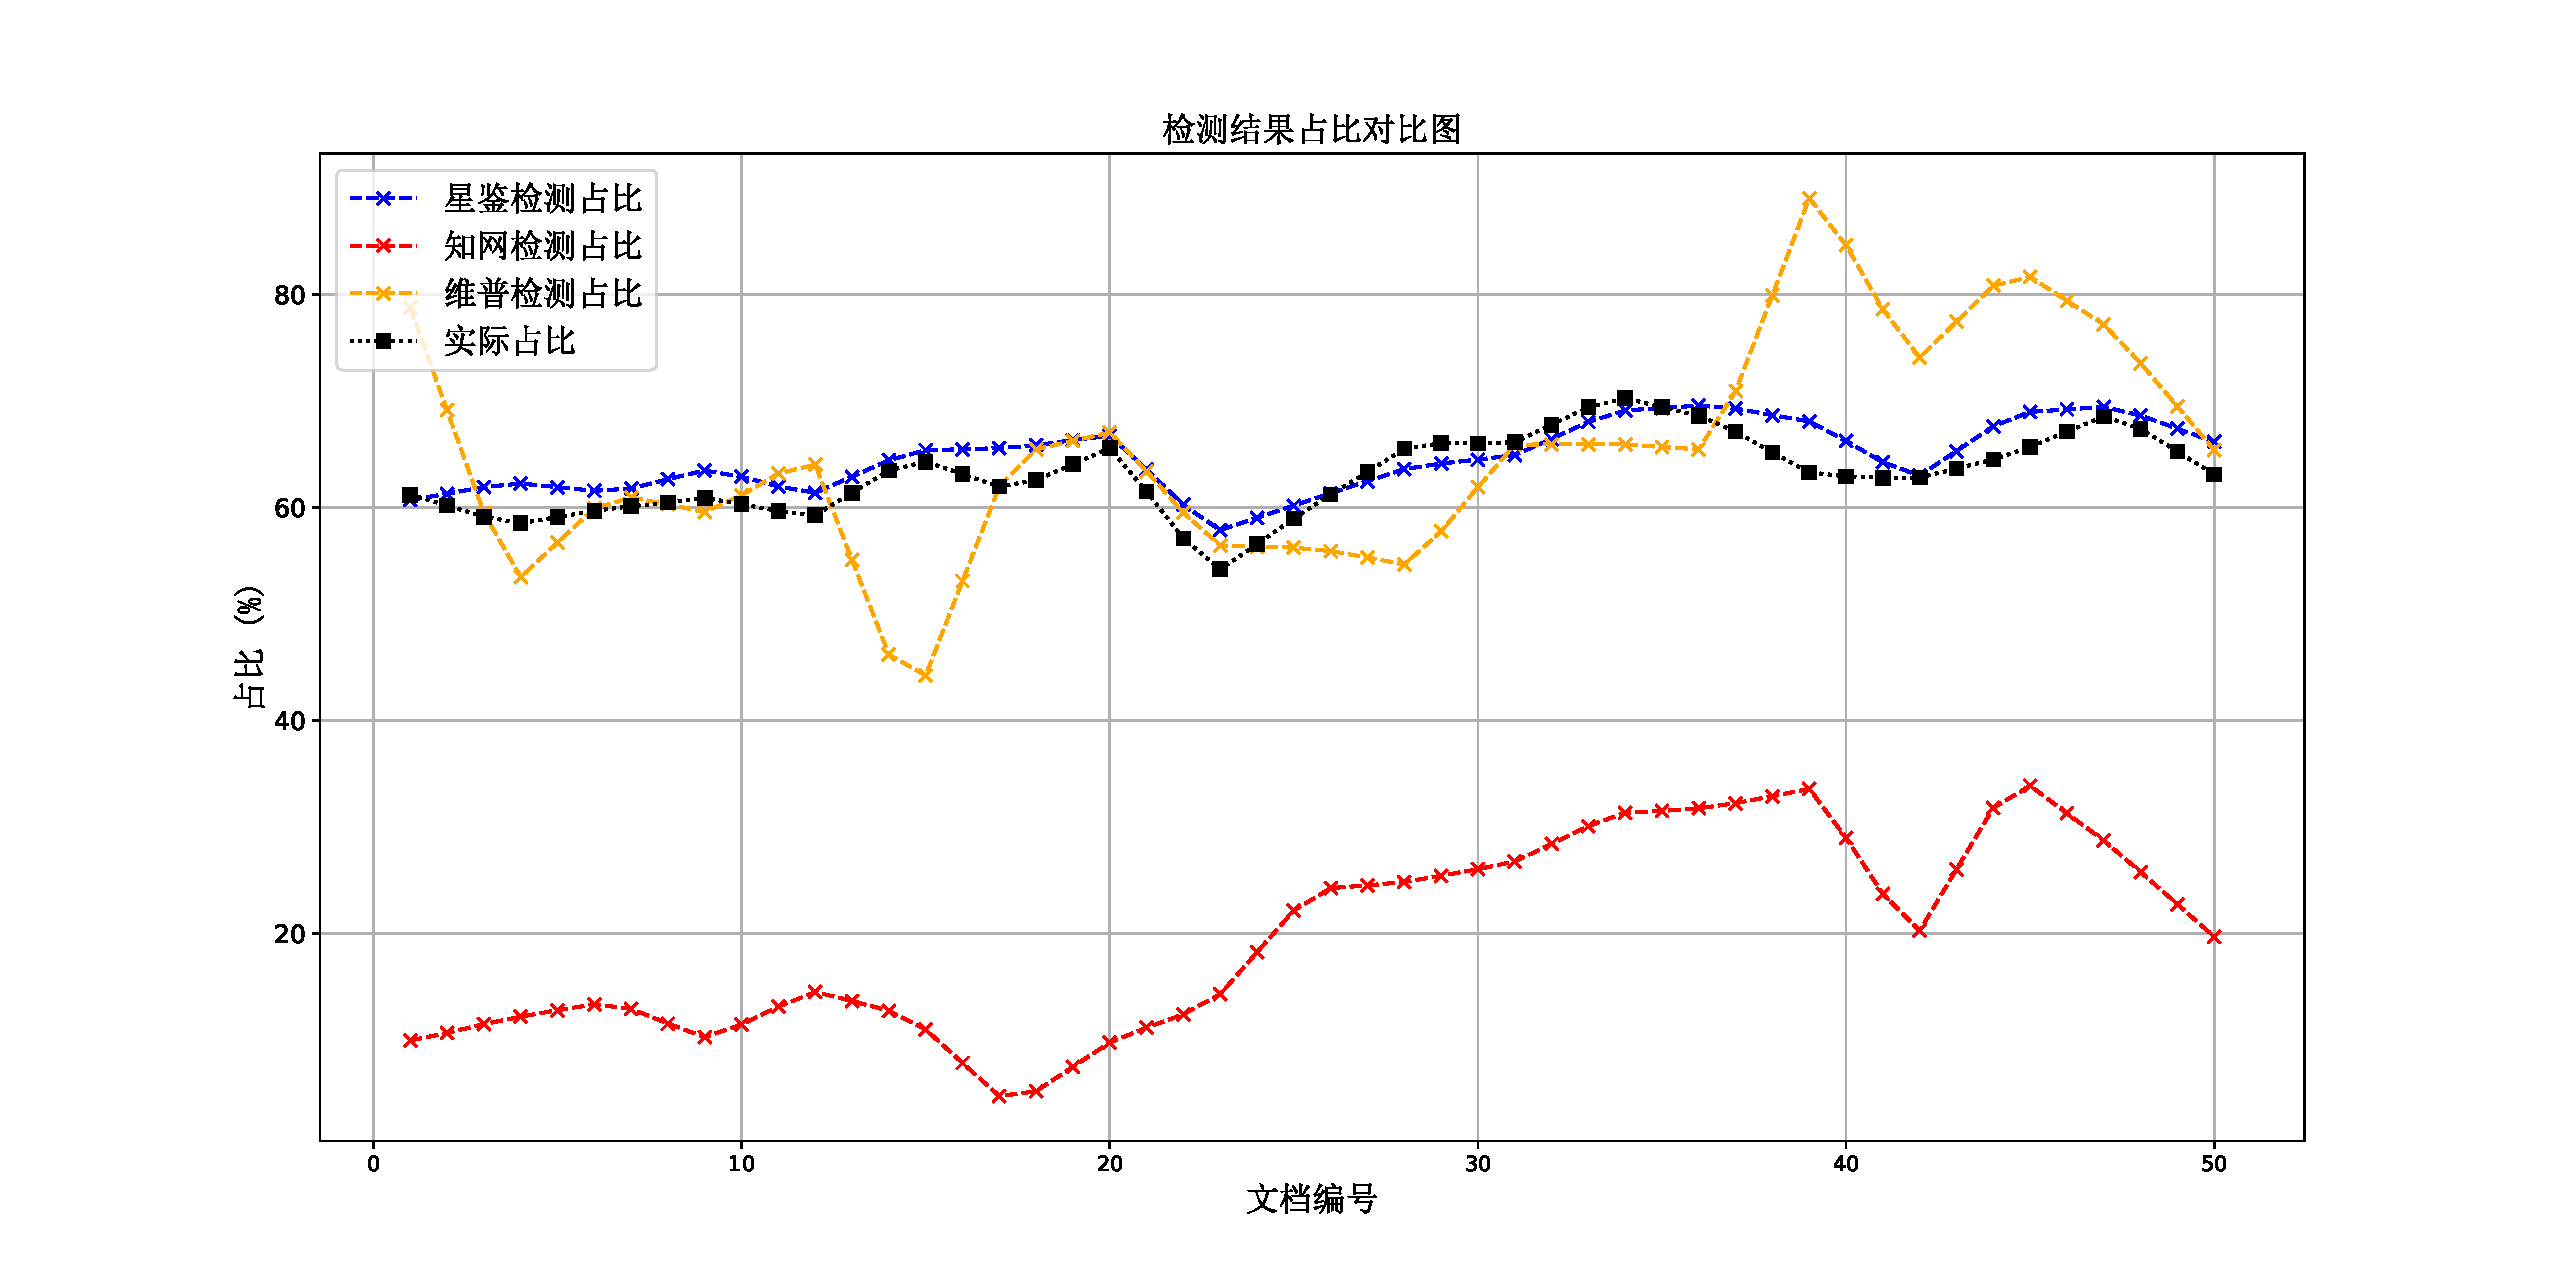
\includegraphics[width=\textwidth]{figures/星鉴性能对比图.pdf}
	\caption{星鉴,知网,维普检测性能比较}
	\label{星鉴,知网,维普检测性能比较}
\end{figure}
如图\ref{星鉴,知网,维普检测性能比较}所示,黑色的折线代表着文章时间的机器生成文本占比,剩下的三条折线代表三种检测系统检测出来的占比。
\begin{itemize}
	\item \textbf{知网}:知网的检测效果似乎并没有达到他宣传的强大算法应该做到的水平,出现了大量漏判的情况,即很多由机器生成的文本都无法检测出来,检测效果不好。同时检测效果似乎和论文领域以及内容关系较大,某些领域例如计算机的论文检测效果略优,但是某些领域例如医学领域的论文检测效果就非常差。
	\item \textbf{维普}:维普的检测效果优于知网,但是错判的情形大量出现,把人类撰写文本误判成机器生成文本,在统计情形中最坏的是一篇2017年发表的论文,这篇论文中有70\%的内容被判成由机器生成,ChatGPT于2022年11月发布,所以一篇2017年的论文是由机器生成的这件事是不可思议的。
	\item \textbf{星鉴}:星鉴的检测效果基本上全分布在实际占比曲线的附近,偏离很少,没有出现明显漏判和错判的情形。
\end{itemize}

我们统计三种检测系统检测出来的机器文本占比和实际机器文本占比的绝对距离以及方差,绘制如下表格
\begin{table}[H]
	\centering
	\begin{tabular}{lcc}
		\toprule
		\textbf{检测系统} & \textbf{平均检测差距} & \textbf{方差} \\
		\midrule
		星鉴            & 2.01            & 1.07        \\
		知网            & 43.32           & 50.45       \\
		维普            & 6.84            & 41.83       \\
		\bottomrule
	\end{tabular}
	\caption{三种检测系统检测效果对比}
	\label{tab:检测系统比较}
\end{table}

通过图\ref{星鉴,知网,维普检测性能比较}以及表\ref{tab:检测系统比较},我们可以看到目前已经商用的AIGC检测系统,知网的检测效果是最不理想的,很难保证可以准确检测学术论文的真实性,作为一个大规模商业使用的检测系统是不太合格的。维普的检测效果优于知网,但是误判的情形太严重,容易把正常的人类撰写文本判断成机器生成文本,这种一棒子打死的策略是很不合理的。
星鉴无论是在漏判还是误判的出现,都远远优于两种商业模型,而且漏判和误判的偏差的比例都极小,检测效果很稳定。
\subsubsection{星鉴,知网,维普检测速度对比}
为了保证检测速度比较的公平性,我们选择了多个时间点对这些文章进行检测,最终我们发现夜间凌晨的时候检测速度最快,此时用户访问较少服务器资源应该比较充裕,因此选取的检测时间都是每一篇文章检测最短的时间即在夜间凌晨时检测文章所需的时间。同时考虑不可能只有一名用户访问知网和维普的服务器,我们在星鉴的服务器模拟了50个用户的高并发,且维普和知网上传文件以及检测文件时两个独立的过程,所以仅统计检测文件需要消耗的时间,最后50篇文章的检测时间对比如图所示:
\begin{figure}[H]
	\centering
	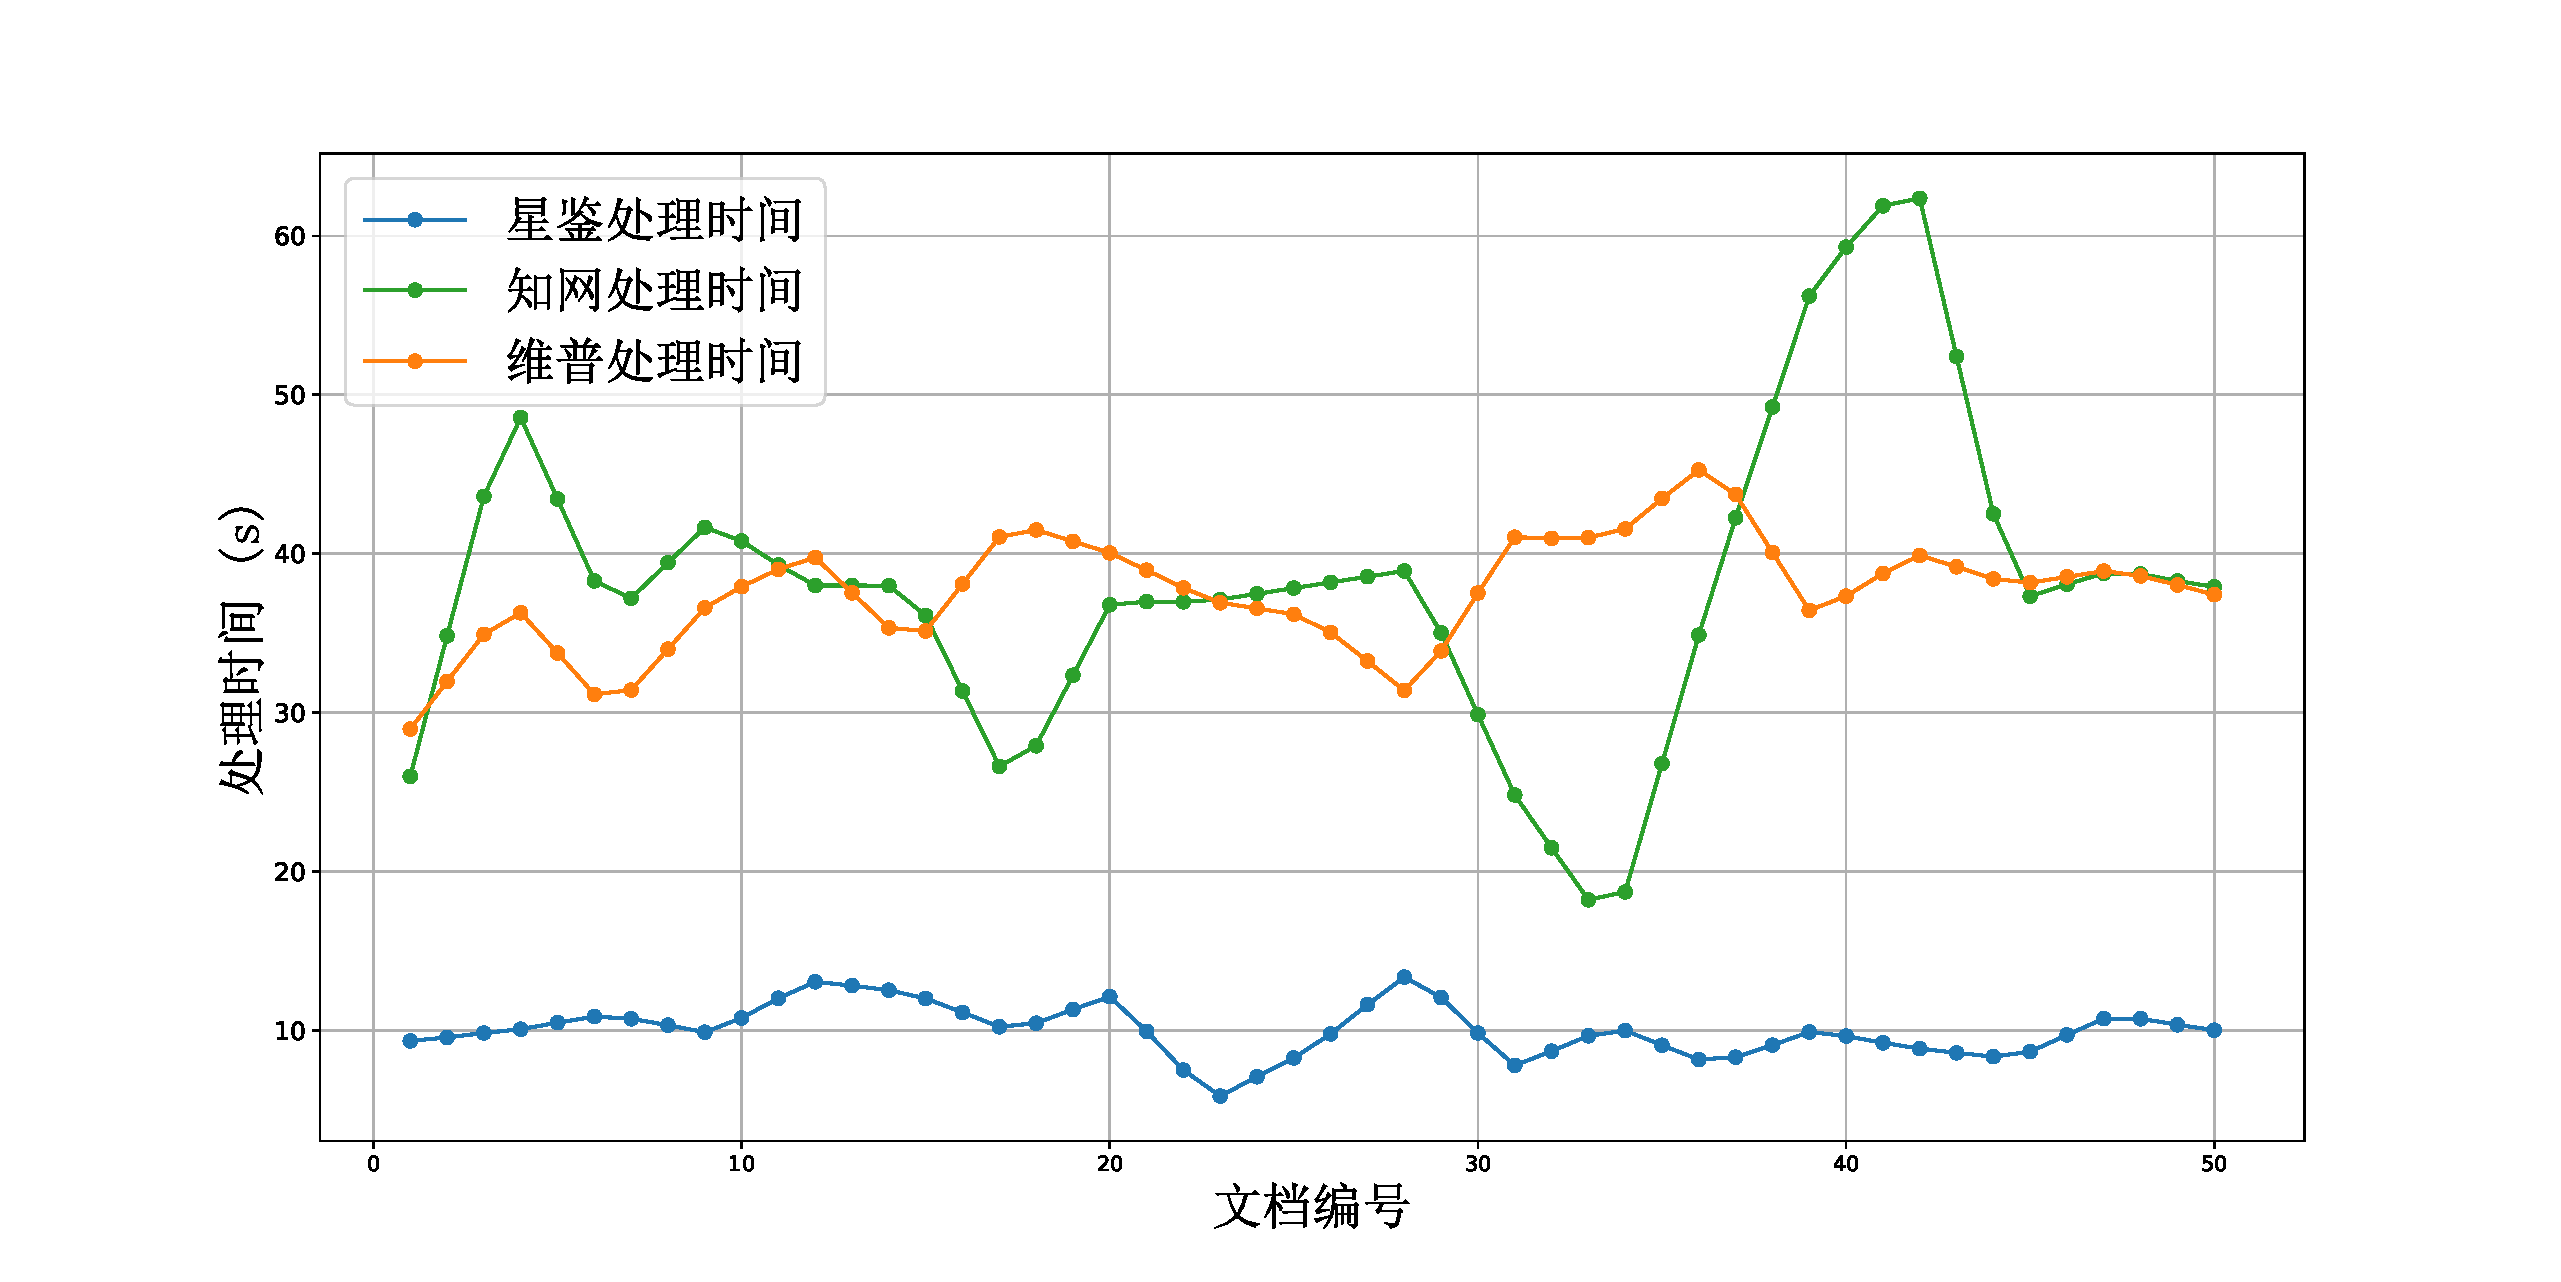
\includegraphics[width=\textwidth]{figures/星鉴速度对比图.pdf}
	\caption{星鉴,知网,维普检测速度对比}
	\label{星鉴,知网,维普检测速度对比}
\end{figure}
从图\ref{星鉴,知网,维普检测速度对比},维普的服务器计算资源似乎比较稳定,字数相同的文章的检测时间也差不多;知网的服务器计算资源波动可能非常大,检测时间和检测字数不完全符合一种正相关的关系,而且综合检测效果曲线来看,似乎检测时间较长的几篇检测效果也比较好,可以猜测知网的检测方法似乎和\textbf{内容领域}有关。星鉴检测的速度远超维普和知网,在50个用户的并发的情况下一万字左右的文档耗时仅需10秒左右,如果在服务器本地进行检测,事先载入文档,优化文件的打开关闭操作,1分钟可以检测100篇1万字的文档,如果考虑一个高校一年有5000篇5万字的毕业论文,那么检测时间也\textbf{不会超过5个小时},如果采用更强大的GPU(例如RTX4090或者A100),时间还可以减少数倍。
\chapter{创新性分析}
\section{技术创新}
\subsection{结合监督学习与零样本检测方法的二元文本分类模型}
机器生成文本检测的方法主要分为白盒检测和黑盒检测。黑盒检测方法可以分为监督学习方法和零样本检测方法两种,监督学习方法在域内检测性能极高,但是泛化性不好,域外性能不佳。零样本检测方法利用预训练语言模型在大规模通用人类文本进行训练的特点具有极高的泛化性,但是检测性能不如域内的监督学习方法,同时检测速度远慢于监督学习。

我们结合了监督学习检测快域内性能强的特点以及零样本检测的泛化性强的特点,构建了\textbf{高效准确的二元文本分类模型}。

由于监督学习的特性,域内数据在设置置信度0.99的情形下,置信区间为 $[0, 0.4357)\cup(0.6621, 1]$,域外数据在设置置信度为0.99的情形下,置信区间为 $[0, 0.2415) \cup(0.7926, 1]$,因此最终选择$[0,0.2)\cup(0.8,1]$作为置信区间,这样域内外的数据都可以达到0.99的置信度。

在区间内的高置信度数据使用监督学习分类器进行二元分类,监督学习方法保证了告诉和高准确性;在区间外的低置信度数据则交给零样本检测分类器,零样本检测良好的泛化性保证了低置信度数据鉴别的高准确性。

“星鉴”系统通过监督学习与零样本检测的巧妙结合,实现了高效且精准的文本分类,能够在实际应用中准确快速的区分人类生成和机器生成的文本。

\subsection{监督学习模块}
传统监督学习的一般做法是选择一个预训练模型作为特征提取器,利用提取出的嵌入层高维向量进行分类决策;但是这一方法有两个严重缺陷:
\begin{itemize}
	\item 域外检测效果不佳,泛化性差
	\item 对新语言扩展性差的缺陷,每增加一种新的语言都需要添加一个该语言版本的预训练模型以及分类模型
\end{itemize}

针对多语言扩展难的问题,“星鉴”选择XLM-RoBERTa-Base多语言版本自编码器预训练语言模型,采用多语言(“星鉴”主要聚焦于英文与中文)的标记数据进行训练,不仅提高了泛化性,而且在进行语言扩展时只需要添加少量对应语言的标记数据即可。

这种创新的做法使得“星鉴”的监督学习模块可以轻松的拓展到多个语言,无需使用不同语言的预训练模型,无需训练多个分类器,保证了监督学习模块的轻量化。

\subsection{零样本检测模块}
传统的零样本检测方法对的调用的预训练模型有很高的性能要求,例如Fast-DetectGPT调用的模型是GPT Neo-2.7B,对GPU的要求很高,需要占用大量的显存。而当我们尝试使用较小的模型时,Fast-DetectGPT使用的“条件曲率”指标区分文本的能力急剧下降,甚至完全丧失区分能力。

针对这一缺陷,我们设计了自信息丰富度(self-information richness,SIR)这一指标,SIR不仅能够在使用小模型的情况下保持较高的区分能力,还能在采样的同时完成SIR的计算,一次检测仅需\textbf{一次模型调用},加快了检测速度。

SIR这一指标的使用,使得“星鉴”不仅能在使用较小的模型(Qwen2-0.5B,调用仅需占用4GiB显存),方便部署的同时实现很好的检测性能,显著降低了检测时的性能压力,极大地提升了检测速度。

同时零样本检测的方法彻底解决了监督学习泛化性差的问题,同时和监督学习相结合吸取了监督学习速度极快的优点,最终实现了一个\textbf{高效准确的二元文本分类模型}。
\section{工程创新}
\subsection{瀚海数据集}
\textbf{针对中文数据集匮乏的问题,我们构建了包含十个大类、超过50个话题的中文数据集,同时覆盖了当前各类主流模型,提高了模型检测的效果。}
在构建二元文本分类检测系统监督学习模块时,数据集的质量直接影响训练出来的检测模型的检测效果。而现有的中文数据集主要来源于HC3,M4会存在领域覆盖面小,以及数据集来源少的两种致命缺陷。例如M4数据集在中文领域只有百科和网页问答两个领域,HC3数据集所有的机器回答都来自ChatGPT。

基于以上数据集训练出的检测模型存在两个问题,\textcircled{1}由于数据集自身涵盖的领域较少,所以检测模型对跨领域的机器生成文本检测能力不强。\textcircled{2}数据集的来源单一,大多都来自于ChatGPT,导致对于其他的大模型生成文本的检测效果不佳。

针对上述问题,我们构建了一个包含十个大类、超过50个话题的中文数据集---“瀚海”数据集,涵盖学术与专业文献、生活与日常、新闻与媒体、艺术与文化、商业与经济、科技与创新等领域。我们不仅扩展了数据集的领域覆盖范围,还从包括Claude3、ChatGPT,文心一言,讯飞星火,通义千问等多个大模型中提取数据,使得数据来源多样化,助力实现文本检测工具的跨领域和跨模型的高效检测,提高检测系统的泛化性。

通过这些努力,我们一定程度上缓解了中文数据集匮乏和多模型输出不足的问题,在中文文本检测中做出了开创性的工作。同时我们的工作也为未来的中文机器生成文本检测研究和应用提供了坚实的基础,并展示了在多语言和多模型环境下提升检测工具性能的可行路径。未来,我们将继续优化和扩展数据集,进一步提升模型的检测能力和泛化性能,为更多的应用场景提供可靠的技术支持。

\subsection{瀚海Benchmark}
\textbf{针对中文领域机器生成文本检测方法的公认性能评估方法匮乏的问题,我们构建了包括七个领域,覆盖所有主流大语言模型的瀚海Benchmark,可以作为中文领域机器生成文本检测的性能基准测试。}

在机器生成文本检测领域,Benchmark实际上就是一个分类模型在一个由人类撰写文本和机器生成文本组成的数据集上测试分类性能。在英文领域的生成文本检测Benchmark已经比较成熟,有很多公开并被广泛使用的数据集用于测试,但是中文领域的生成文本检测领域的Benchmark几乎是一片空白,因此我们在“瀚海”数据集的基础上,进一步设计并构建了“瀚海”中文Benchmark,用于中文生成文本检测模型的性能测试。

“瀚海”中文Benchmark涵盖学术,新闻,评论,诗歌,医疗,对话,动态等七个领域,包含了超过5000条中文人类撰写文本和机器生成文本的对比条目,调用了国内外一系列大模型包括ChatGPT,Claude3,讯飞星火,文心一言,通义千问,Kimi的API,采取了一系列Prompt工程进行构建。

“瀚海”Benchmark涵盖了多个领域,覆盖了目前的主流大语言模型,为后续的中文领域机器生成文本检测方法提供了性能检测的方法,同时也可以作为行业的一项性能基准测试,为后续检测方法的性能提升提供指引。


\chapter{总结与展望}
\section{作品总结}
“星鉴”机器生成文本检测系统是当前中文领域机器生成内容检测的实用解决方案,其拥有极高的准确率、处理速度以及简洁美观的用户反馈界面。“星鉴”创新地将监督学习和零样本检测相结合的方法引入文本分类功能,结合"瀚海"数据集进行训练,最终在多模型多领域中英文环境下的机器生成文本检测中表现优秀。

数据方面,我们构建了包括多领域多模型的中文人类机器文本数据集---“瀚海”数据集,涵盖学术与专业文献、生活与日常、新闻与媒体、艺术与文化、商业与经济、科技与创新等领域,覆盖ChatGPT,Claude3,讯飞星火,文心一言,通义千问,Kimi等主流大语言模型,同时基于“瀚海”数据集,我们还构建“瀚海”Benchmark,为后续的中文领域机器生成文本检测方法提供了一项性能基准测试。

功能方面,“星鉴”机器生成文本检测系统支持直接输入文本检测和上传文件检测。针对文本检测,“星鉴”不仅提供了文本整体的机器生成概率,还引入了人类文本,疑似机器文本以及机器文本的占比环形图和段落级别的概率标记,让用户能够直观地了解内容的真实性分布。针对文件处理,“星鉴”支持PDF、TXT、DOCX等常见文本格式,同时支持提取图片中文字的功能,并且能给出详细的检测报告和全文不同段落部分的标记,为用户的内容审核提供了综合分析和精准指引。

平台实现方面,“星鉴”机器生成文本检测系统包括网页端,Windows本地端应用,Android端引用。网页端星鉴检测系统支持全平台所有操作系统访问,给所有用户提供文本检测功能。Windows本地端应用支持用户利用本地算力,无需联网上传数据,重视保护数据隐私安全。Android端应用基于云计算,给用户提供随时随地,一键点击即可轻松使用的机会。系统源代码开源,任何人都可以基于源代码进行改进,实现更好的检测效果或者功能个性化定制。


安全性方面,"星鉴"同样表现出色。我们对“星鉴”进行了攻击分析与测试,证实了系统具有强大的抗攻击能力,有效防范了各种潜在的欺骗手段,确保检测结果的可靠性和稳定性。

最后我们对“星鉴”检测系统进行了综合测试,并和市面上目前商用的一些AIGC检测系统进行对比。结论显示“星鉴”在中文领域检测效果、处理时间等多个指标上全面超越当前已商用的知网、维普等机构的AIGC检测系统。

“星鉴”在中文内容的机器生成文本检测领域展现了卓越的性能,有效地填补了现有工具针对中文机器生成内容检测的空白。秉持着开源精神以及科技普惠的原则,我们对源代码进行开源并且任何用户都可以免费使用检测系统以及在本地自己部署属于自己的文本检测系统。这一策略大幅降低了内容审核的经济负担,无论是科研机构、教育部门,还是媒体从业者,都能轻松地利用“星鉴”来监测机器生成文本。同时“星鉴”在内容安全方面同样具有广阔的应用前景。政府机构、企业安全部门以及内容平台的审核团队等均可利用这项技术,辅助追踪发布内容的来源,从而有效防范机器生成的虚假信息的传播,控制网络舆论的正确导向,保障内容生态的健康发展。“星鉴”的全面推广与应用,将有助于构建一个更加真实、可信和安全的中文网络环境,为社会的和谐与稳定贡献力量。
\section{未来展望}
\subsection{数据集扩展}
我们计划将“瀚海”数据集从现有的中文版本扩展到多种语言版本,以适应当今全球多样化的需求。我们的目标是创建一个多元语言的数据集,涵盖英语、俄语、阿拉伯语、法语等,为检测系统覆盖更广泛的语言应用场景提供支持。同时我们还将进一步扩展数据来源,细分数据标签,使得数据集能够涵盖更多的领域和话题,并且从更多的大语言模型收集更多的数据。未来随着大模型的不断迭代,我们数据集的内容也将不断实时更新。这将有助于提升检测系统在不同语言,领域以及不同模型的检测能力,并随着大模型的迭代不断提升自身检测能力,从而提高文本检测的准确性和鲁棒性以及泛化性。
\subsection{提升可移植性}
目前检测系统可以在Windows系统上直接运行,使用源码也可以在Linux以及macOS系统上运行。我们计划后续开发出适配目前除Windows以外所有主流操作系统的应用程序而不借助于源代码和python环境,包括macOS,ios以及即将发布的国产自研的HarmonyOS Next操作系统,实现“星鉴”机器生成文件检测系统的全平台部署。


% 打印参考文献
\bibliographystyle{unsrt} % 使用 unsrt 样式
\bibliography{references}
\addcontentsline{toc}{chapter}{参考文献}
\chapter*{附录}
\addcontentsline{toc}{chapter}{附录}
\section*{“瀚海”数据集展示(部分)}
\addcontentsline{toc}{section}{“瀚海”数据集展示(部分)}
\begin{lstlisting}[language=json]
{"label":"news","human_answers":["本场比赛,波尔津吉斯复出替补出战。首节比赛,面对老东家的波尔津吉斯连续砍分,......"],"robot_answers":["新闻标题:波尔津吉斯率领凯尔特人大胜独行侠,一场精彩的篮球对决\n\n新闻正文:......"],"model":ERINE}
{"label": "news", "human_answers": ["小米MIX Fold 4折叠屏手机通过工信部入网审核,支持天通卫星通信......"], "robot_answers": ["新闻稿:\n\n标题:小米MIX Fold 4折叠屏手机通过工信部入网审核,将支持天通卫星通信\n\n日期:XXXX年X月X日\n\n小米公司近日迎来重大突破,其......"], "model": "ERINE"}
{"label": "news", "human_answers": ["阿斯麦CEO警告:美遏华或起反效果随着美国逐步收紧对中国出口先进芯片和芯片制造工具的管制,荷兰光刻机巨头阿斯麦成为国际政治博弈......"], "robot_answers":[ "【全球芯片产业震荡:阿斯麦CEO发声警惕美对华芯片限制反噬效应】\n\n全球领先的光刻机制造商荷兰阿斯麦(ASML)的首席执行官......"], "model": "qwen1.5-110b-chat"}
{"label": "news", "human_answers": ["波利塔诺不适合孔蒂的战术要求 可能遭弃用离队北京时间6月6日, 有媒体曝料,那不勒斯新主帅孔蒂上任后可能会导致边锋波利塔诺......"], "robot_answers": ["【那不勒斯讯】6月6日,意大利足坛再起波澜,有关那不勒斯边锋波利塔诺未来的猜测甚嚣尘上。据最新媒体报道,随着孔蒂执掌......"], "model": "qwen1.5-110b-chat"}
{"label": "news","human_answers": ["本场比赛,波尔津吉斯复出替补出战。首节比赛,面对老东家的波尔津吉斯连续砍分......"], "robot_answers": ["标题:波尔津吉斯复出闪耀凯尔特人大胜独行侠\n\nXXXX网 XXXX年XX月XX日\n\n在一场充满激情和对抗的NBA常规赛中,凯尔特人队"], "model": "xinghuo"}
{"label": "news", "human_answers": ["继续征战CBA?克里克结束休假返回中国训练北京时间6月5日消息,2023-2024赛季CBA联赛已经落下帷幕......"], "robot_answers": ["标题:克里克休假结束返京训练,考虑留CBA继续征战\n\nXXX报 XXXX年XX月XX日\n\n在2023-2024赛季CBA联赛落下帷幕后......"], "model": "xinghuo"}
{"label": "news", "human_answers": ["宁德时代发布声明:美国会议员有关强迫劳动的指责是毫无根据和完全错误......"], "robot_answers": ["6月5日,一些美国国会议员致信指控宁德时代的供应链涉及强迫劳动。对此,宁德时代于6月7日晚发表声明......"], "model": "Claude3 Sonnet"}
{"label": "news", "human_answers": ["特斯拉中国上线百度地图V20财联社6月7日电,百度地图V20真车道级导航全球首发......"], "robot_answers": ["6月7日,百度宣布其最新版本的地图导航系统——百度地图V20在......"], "model": "Claude3 Sonnet"}
{"label": "news", "human_answers": ["AI工具\"Recall\"安全性受质疑,微软紧急加强防护微软公司近日宣布,\"Recall\"的新功能将默认设置为关闭状态。......"], "robot_answers": ["微软公司近日宣布,他们将对新推出的AI工具"Recall"加强防护措施。此工具曾被网络安全专家质疑可能会成为黑客的目标,因此微软决定在默认设置下关闭该功能。......"], "model": "ChatGPT4o"}
{"label": "news", "human_answers": ["理想郎咸朋确认智驾裁员结束:\"再走一个人,优先走的那个人是我\"21世纪经济报道从多个信源获悉,6月7日上午......"], "robot_answers":  ["根据最近的报道,理想汽车创始人兼CEO李想确认公司的智驾部门裁员已经结束......"], "model": "ChatGPT4o"}
{"label": "law", "question": "被非法拘禁侮辱。当年报警,派出所不肯立案,也不肯给不予立案通知书。最后没办法不了了之......", "human_answers": ["先别着急确定这个5年的时效,考虑:1、非法拘禁中侮辱情节,是否具有身体伤害,是否构成重伤......"], "robot_answers":["非常理解你的遭遇和此刻的无奈心情。面对这种情况,确实需要采取一些行动来维护自己的合法权益......"], "model": "ERINE"}
{"label": "law", "question": "同一栋楼,发现自己买的价格要比本地人或其他人高出很多,请问这在法律上属于合理还是有欺诈或欺骗消费者行为......", "human_answers": ["房子有商品属性"], "robot_answers": ["一般来说,购买房产的价格是根据市场供需、地理位置、房屋状况、建设质量等因素决定的。如果在同一栋楼内,发现自己购买的房产价格明显高于本地人或其他购房者......"], "model": "ERINE"}
{"label": "law", "question": "提前预定酒店,酒店有规则超过半小时就不能取消了,这种规则有法律效力吗?超过半小时后但是提前十天取消这种能正常取消吗?", "human_answers": ["那这个规则不就加重了消费者的责任了吗,而且这么强的约束力平台在预定的时候应该给用户强提示告知吧"], "robot_answers": ["酒店的预订取消政策通常是由酒店自行设定并在预订时明确告知顾客的。这种规则在法律上是具有约束力的,前提是它在预订过程中被清晰、显著地展示给消费者,并且消费者在预订时同意了这些条款......"], "model": "qwen1.5-110b-chat"}
{"label": "law", "question": "博四了,学校后勤搞事,从博一开始把博士宿舍一人间改六人间,使得所有博士无法毕业,人生被毁,投诉多次无果,无数家庭的希望被摧残,如何起诉学校维权?", "human_answers": ["学校博士管理章程里面有规定吗?有的话可以起诉索赔试试,但胜诉可能不大"], "robot_answers":[ "面对这样的情况,首先需要冷静分析并采取合理合法的步骤来解决问题。以下是一些建议的步骤,但请注意......"], "model": "qwen1.5-110b-chat"}
{"label": "law", "question": "比如说同事之间发生口头矛盾,双方互骂。这时候其中一方从扣腰带里抽出一把折叠刀威胁说,你再骂一个试试......", "human_answers": ["如果你并不是法律专业人士,其实没必要去生搬硬套法律术语,相信你自己的直觉就是了。你要......"], "robot_answers": ["在法律上,犯罪预备通常指的是一个人准备或企图实施一个犯罪行为......"], "model": "xinghuo"}
{"label": "law", "question": "老公偷偷补贴爸妈违法吗?", "human_answers": ["从情理上来说,孝顺父母是理所应当的,但从法律上来看,婚后夫妻双方的收入......"], ["robot_answers": "在法律层面,夫妻婚后的财产被视为共同财产,根据《民法典》的规定,任何一方都无权单独对共同财产进行处分......"], "model": "xinghuo"}
{"label": "law", "question": "我妈妈在厂里上班,厂里包住是一人一个宿舍第二天没去上班,打电话没人接工友来找我妈妈敲门没反应......", "human_answers": ["先确认死因,然后确认是哪种劳动关系,在进行是否是工伤,再进行后续的赔偿问题"], "robot_answers": ["我非常抱歉听到您母亲的噩耗。在这种悲痛的时刻,请接受我最诚挚的慰问。您正面临着一个复杂而困难的情况......"], "model": "Claude3 Sonnet"}
{"label": "law", "question": "1月初入职新公司,现在6月4号通知6月20号辞退我,是公司单方面项目原因,本人没有任何过错,怎么要求公司赔付金额,这个时间算满6个月......", "human_answers": ["首先,工资肯定是可以要的,和解除与否无关。关于公司解除合同行为,如果不在试用期且本人无过错,可以要求N+1,走违法解除的法律依据赔偿是2N,还没有N+1多。"], "robot_answers": ["根据您提供的信息,我理解您的情况如下:1. 您于1月初入职新公司。2. 公司于6月4日通知您,将在6月20日辞退您。3. 辞退原因是公司单方面的项目原因,......"], "model": "Claude3 Sonnet"}
{"label": "law", "question": "15岁骑共享单车正常直行,但是载了2个人,撞到了人行道转弯出来的电动车前轮,对方要求赔偿所有修理费用,这种责任该怎么划分啊?", "human_answers": ["第一,报警,让交警出责任认定书第二,15周岁已经允许骑自行车了......"], "robot_answers": ["在这种情况下,责任的划分需要考虑多个因素,包括交通法规、事故发生的具体情况以及双方的过错。......"], "model": "ChatGPT4o"}
{"label": "law", "question": "我在电商卖货上班,原价900(本钱480)的单价我上成了99,一共有10单,总共8000(本钱共4800),需要赔偿吗,没有故意上错,只是工作劳累失误了", "human_answers": ["一般损失不用赔偿 重大损失当月工资百分之20"], "robot_answers": ["在这种情况下,是否需要赔偿通常取决于你所在公司的政策和相关的劳动法律法规。以下是几个需要考虑的因素:......."], "model": "ChatGPT4o"}
\end{lstlisting}





\end{document}
